% This is samplepaper.tex, a sample chapter demonstrating the
% LLNCS macro package for Springer Computer Science proceedings;
% Version 2.21 of 2022/01/12
%
\documentclass[runningheads]{llncs}
%
\usepackage[T1]{fontenc}
% T1 fonts will be used to generate the final print and online PDFs,
% so please use T1 fonts in your manuscript whenever possible.
% Other font encodings may result in incorrect characters.
%
\usepackage{graphicx}
% Used for displaying a sample figure. If possible, figure files should
% be included in EPS format.
%
% If you use the hyperref package, please uncomment the following two lines
% to display URLs in blue roman font according to Springer's eBook style:
%\usepackage{color}
%\renewcommand\UrlFont{\color{blue}\rmfamily}
%\urlstyle{rm}
%
\usepackage{hyperref}
\usepackage{booktabs} % To thicken table lines
\usepackage{multirow}
\usepackage{pgf}
\usepackage{makecell}
\usepackage{algorithm} 
\usepackage{algpseudocode} 
\usepackage{amsmath} 

\begin{document}
%
\title{Learning to Select Promising Initial Solutions for Large Neighborhood Search-Based Multi-Agent Path Finding\thanks{This project is partially funded by the Doctoral Program ``Vienna Graduate School on Computational Optimization'', Austrian Science Foundation (FWF), grant W1260-N35.}}
%
\titlerunning{Learning to Select Promising Initial Solutions for LNS-based MAPF}
% If the paper title is too long for the running head, you can set
% an abbreviated paper title here
%
\author{Marc Huber\inst{1}\orcidID{0009-0003-2862-6232} \and
Günther R.\ Raidl \inst{1}\orcidID{0000-0002-3293-177X} \and
Christian Blum\inst{2}\orcidID{0000-0002-1736-3559}}
%
\authorrunning{M.~Huber, G.~R.~Raidl, and C.~Blum}
% First names are abbreviated in the running head.
% If there are more than two authors, 'et al.' is used.
%
\institute{Institute of Logic and Computation, TU Wien, Austria \\
\email{\{mhuber,raidl\}@ac.tuwien.ac.at}\\
\and
Artificial Intelligence Research Institute (IIIA-CSIC), Campus of UAB, Spain\\
\email{christian.blum@iiia.csic.es}}
%
\maketitle              % typeset the header of the contribution
%
\begin{abstract}

Anytime Multi-Agent Path Finding (MAPF) is a promising paradigm for finding fast and (near-)optimal solutions to large-scale multi-agent systems within a fixed time budget. The currently leading approach builds on Large Neighborhood Search (LNS), which iteratively optimizes a quickly generated initial solution by repeatedly selecting and replanning paths of subsets of agents using randomized destroy heuristics and Prioritized Planning (PP). In this study, we examine the impact of initial solutions on the quality of final solutions in a state-of-the-art LNS-based anytime MAPF algorithm. Our findings demonstrate that its effectiveness is significantly influenced by the choice of the initial solution. Building on this insight, we propose to run PP many times to create a larger pool of potential initial solutions, from which we then select by means of an offline-trained Machine Learning (ML) model a most promising solution to run the LNS on. Empirical results on well-established MAPF benchmark instances show that the ML model successfully selects a most promising solution from the pool of potential initial solutions. This leads to improved performance of the state-of-the-art LNS-based anytime MAPF method in terms of both the final solution quality and the Area Under the Curve when initiated from the selected solution.

\keywords{Anytime Multi-Agent Path Finding  \and Machine Learning \and Large Neighborhood Search.}
\end{abstract}
%
%
% Reset footnote counter
\setcounter{footnote}{0}

\section{Introduction}

Finding a set of collision-free paths for a group of agents in a shared environment has many important contemporary real-world applications, including automated warehouses~\cite{wurman-2008}, robotics, and autonomous vehicles~\cite{veloso-2015}. In computer science, this problem is known as the Multi-Agent Path Finding (MAPF) problem~\cite{stern-2019}. Desirable solutions to the MAPF problem are those which are  conflict-free, but also minimize some objective function. However, finding optimal solutions under various objective functions, such as the sum of costs, has proven to be NP-hard~\cite{yu-2013}, as the state-space grows exponentially with the number of agents. In practice, attempts to solve MAPF instances with a few hundred or more agents using exact or reasonably bounded suboptimal MAPF algorithms typically requires far too much time or memory. In contrast, fast constructive heuristics usually only find low-quality solutions or no feasible solutions in tightly constrained scenarios at all. To address these issues, researchers have explored anytime MAPF approaches~\cite{cohen-2018,li-2021,lam-2023} which combine the strengths of both worlds. Anytime algorithms aim to find feasible solutions quickly and then continuously work on improving them as long as time remains, possibly converging to optimality if time allows.

In the context of anytime MAPF algorithms, Large Neighborhood Search (LNS)-based MAPF is a promising approach that relatively quickly finds solutions to the MAPF instances and iteratively improves them to near-optimality by repeatedly selecting and replanning paths of subsets of agents using destroy and repair heuristics~\cite{li-2021}. The subset of agent paths selected for replanning is referred to as a neighborhood. If the newly found solution is superior to the incumbent solution, the incumbent solution is replaced by the new solution. This iterative process continues until an allocated time budget is exhausted.

MAPF-LNS~\cite{li-2021} is the currently leading LNS-based approach for anytime suboptimal MAPF solving. It first produces an initial solution quickly using an efficient MAPF construction heuristic. Then, MAPF-LNS repeatedly applies randomized destroy heuristics and replans paths of subsets of agents using Prioritized Planning (PP)~\cite{silver-2005} with random
priorities to further improve the solution until the allotted time is exhausted.

While MAPF-LNS has been empirically demonstrated to scale up to large instances with several hundreds of agents, we observed that the quality of the final solution is significantly influenced by the initial solution, even though the quality of the initial solution is not correlated much with the quality of the final~solution. 

This article proposes ISS-MAPF-LNS, the Initial-Solution-Selecting-MAPF-LNS, which aims to enhance MAPF-LNS's ability to find high-quality solutions by initiating the LNS from a more promising initial solution that is selected from a larger pool. The novel aspect of ISS-MAPF-LNS is an offline-trained machine learning (ML) model that selects from a pool of initial solutions generated by PP a most promising solution to run the LNS on. In more detail, a LambdaMART~\cite{burges-2010} model is trained to compute \emph{scores} for the pool of PP-produced initial solutions and we select the most promising solution based on these scores. Thus, the learned scoring function reflects how promising each initial solution candidate is to ultimately get a final solution of highest quality when applying the LNS on~it.

To assess the performance of ISS-MAPF-LNS, we conduct a series of experiments on five well-established MAPF benchmark instances. The results demonstrate that the trained ML model indeed selects a solution being among the most promising ones from the pool of potentially initial solutions, such that the subsequent LNS leads to a lower-cost final solution than MAPF-LNS applied to an average solution. Moreover, the ML model trained on a specific map with 50 agents scales well to the same map and also to unseen maps with hundreds of agents, leading to improved performance over MAPF-LNS on many instances.

The remainder of this article is organized as follows: Section~\ref{sec:problem-definition} formally introduces the MAPF problem, and Section~\ref{sec:related-work} reviews related work. Section~\ref{sec:iss-mapf-lns} empirically analyzes the impact of initial solutions on the quality of final solutions in MAPF-LNS and presents our ISS-MAPF-LNS. Results of computational experiments are discussed in Section~\ref{sec:experiments}. Finally, in Section~\ref{sec:conclusions}, we conclude and outline promising avenues for future research.


\section{Problem Definition} \label{sec:problem-definition}

Multi-Agent Path Finding (MAPF) encompasses a wide variety of variants, as outlined in~\cite{stern-2019}. In this study, we focus on the simplest and most studied variant that considers three key elements: (1) vertex and swapping conflicts, (2) the ``stay at target'' assumption, and (3) the sum of costs objective function. Time and space are discretized.  The input to the MAPF problem is a connected, undirected, unweighted graph $G=(V,E)$, along with a set of $m$ agents $A=\{a_1, \ldots , a_m \}$. Each agent $a_i \in A$ has associated a start vertex $s_i \in V$ and a goal vertex $g_i \in V$ (which may coincide). It is assumed that each start vertex is distinct from all other agents' start vertices and also each goal vertex is distinct from all others. At each discrete time step $t$, every agent is located at one of the graph vertices and can either move to a neighboring vertex or wait at its current vertex. A path $p_i = (p_{i,0}, \ldots , p_{i,l(p_i)})$ for agent $a_i$ is a sequence of neighboring vertices, where $l(p_i)$ is the length of the path $p_i$. An edge $(p_{i,t},p_{i,t+1}) \in E$ indicates a move action, while a vertex $p_{i,t} = p_{i,t+1} \in V$ indicates a wait action. The start vertex is $p_{i,0} = s_i$, while the goal vertex is $p_{i,l(p_i)} = g_i$. It is assumed that an agent remaining at its goal vertex is considered as a wait action if and only if it will subsequently move away from its goal vertex in a subsequent time step before finally returning later. The distance between two vertices, $d(x,y)$, is defined as the length of the shortest path from $x$ to $y$. The delay of path $p_i$ is $\mathrm{delay}(p_i) = l(p_i) - d(s_i,g_i)$. A solution is a set of paths, one for each agent, such that the agents can follow these paths simultaneously without colliding with each other. The objective is to find a solution $P = \{p_i \; | \; a_i \in A \}$ that minimizes its sum of costs, denoted as $\mathrm{SOC}=\sum_{p_i \in P} l(p_i)$, or, alternatively, its sum of delays, denoted as $\mathrm{SOD}=\sum_{p_i \in P} \mathrm{delay}(p_i)$. 


\section{Related Work} \label{sec:related-work}

A fast constructive approach to MAPF is Prioritized Planning (PP)~\cite{silver-2005}, which generates a solution by sorting the agents according to some priority function and subsequently planning a shortest path for each agent iteratively such that agents with lower priority avoid collisions with the already planned paths of higher-priority agents. While being fast, PP often produces low-quality solutions or does not find any feasible solution in tightly constrained scenarios.

Research on anytime MAPF has enjoyed an increasing interest in recent years, due to its practical relevance in finding (near-)optimal solutions within a reasonable time budget. This family of algorithms is particularly advantageous in dynamic and large-scale environments where computational efficiency is crucial~\cite{vedder-2021}. 

In its early stages, several $\mathrm{A}^*$-based algorithms have been proposed. These approaches achieve the anytime behavior either by repeatedly calling $\mathrm{A}^*$ for increasing subproblems~\cite{standley-2011,vedder-2021} or by iteratively tightening the bounds of focal search~\cite{pearl-1982}, as suggested by Cohen~et~al.~\cite{cohen-2018}. However, these approaches are primarily effective for instances that are not congested, as the complexity and number of potential conflicts increase significantly in densely populated environments, leading to excessive computational overhead.

In a recent publication, Li~et~al.~\cite{li-2021} proposed MAPF-LNS, which effectively scales to large instances with hundreds of agents and represents the current leading anytime MAPF approach to date. Given a MAPF instance, the algorithm first invokes an efficient suboptimal MAPF algorithm to quickly find an initial solution $P$. Subsequently, in each iteration, it selects paths of a subset of agents $A_s \in A$ using a randomized destroy heuristic, deletes their paths $P^-_s = \{p_i \in P \; | \; a_i \in A_s\}$ from $P$, and calls PP with random priorities to find a set of collision-free paths $P^+_s$ that also do not collide with paths still in $P$. If the paths in $P^+_s$ have smaller sum of cost than the paths in $P^-_s$, MAPF-LNS adds paths $P^+_s$ to $P$ and $P^-_s$ otherwise. This procedure is repeated until the allocated time budget is exhausted.

Building on the popularity of MAPF-LNS, researchers have proposed several extensions to the original model. Li~et~al.~\cite{li-2022} suggested MAPF-LNS2, which begins with an infeasible solution and repeatedly replans paths of subsets of agents in order to find paths with fewer conflicts. This process is repeated until all paths are conflict-free or the allotted time has elapsed. Huang~et~al.~\cite{huang-2022} proposed MAPF-ML-LNS, which learns a ranking function for a collection of paths, $\mathcal{P} = \{P^-_1, P^-_2, \ldots, P^-_n\}$, generated by the destroy heuristics in MAPF-LNS, such that replanning increases the solution quality more. Specifically, given an incumbent solution, MAPF-ML-LNS generates a collection of paths $\mathcal{P}$, using two randomized destroy heuristics. Then, it applies an offline-trained ranking function to $\mathcal{P}$ and replans the paths in descending order of the predicted scores. If a solution with smaller sum of costs is found, it discards $\mathcal{P}$ and continues to the next iteration. In contrast, Lam~et~al.~\cite{lam-2023} incorporated MAPF-LNS as primal heuristic in branch-and-cut-and-price. This approach combines the strengths of LNS with branch-and-cut-and-price techniques and allows for more efficient resolution of large-scale MAPF problems while still retaining optimality guarantees. Phan~et~al.~\cite{phan-2024} proposed BALANCE, a bi-level multi-armed bandit scheme that dynamically adapts the selection of destroy heuristics and neighborhoods during the search process. This method aims to avoid expensive prior efforts such as data acquisition, model training, and feature engineering by adjusting strategies on the fly based on real-time performance feedback.

Concerning specifically the impact of initial solutions in LNS on the final solution quality, we are unaware of any specific approach in the literature that utilizes ML to learn how to select promising initial solutions for LNS.

\setlength{\tabcolsep}{4.0pt}
\begin{table}[!t]
\caption{Variance and correlation results obtained by MAPF-LNS across various scenarios and maps.}
\label{tab:solution-correlation-variability}
\centering
\scalebox{0.75}{
\begin{tabular}{|c|rrr|rrr|rrr|}
\hline
\multirow{3}{*}{Scenario} & \multicolumn{3}{c|}{\texttt{random-32-32-20}} & \multicolumn{3}{c|}{\texttt{empty-32-32}} & \multicolumn{3}{c|}{\texttt{ost003d}} \\ 
 & \multicolumn{3}{c|}{$m=150$, $N=16$} & \multicolumn{3}{c|}{$m=400$, $N=8$} & \multicolumn{3}{c|}{$m=300$, $N=8$} \\ \cline{2-10}
 & $\sigma$ & $\mu_{\sigma}$ & $r$ & $\sigma$ & $\mu_{\sigma}$ & $r$ & $\sigma$ & $\mu_{\sigma}$ & $r$ \\ \hline

1  & 10.23 & 14.68 & 0.21 & 81.63 & 70.01 & 0.39 & 156.49 & 133.41 & 0.05 \\
2  &  5.99 & 11.98 & 0.24 & 60.04 & 71.11 & 0.05 & 135.85 & 157.30 & 0.62 \\
3  &  6.83 & 12.06 & 0.13 & 71.68 & 85.46 & 0.01 &  58.74 &  96.42 & -0.14 \\
4  &  8.96 & 13.35 & -0.02 & 49.08 & 59.00 & 0.43 &  66.23 &  93.40 & 0.16 \\
5  & 11.21 & 16.58 & 0.15 & 93.45 & 77.15 & 0.51 &  62.13 & 122.33 & 0.04 \\
6  &  7.94 & 13.91 & -0.47 & 83.26 & 67.35 & 0.32 & 139.85 & 133.44 & 0.15 \\
7  & 12.35 & 21.03 & 0.06 & 69.39 & 79.00 & 0.20 & 108.35 & 154.04 & 0.27 \\
8  &  9.89 & 20.08 & -0.16 & 111.42 & 96.67 & 0.67 & 149.77 & 139.49 & 0.24 \\
9  & 12.05 & 18.28 & 0.08 & 74.31 & 73.12 & -0.01 & 112.73 & 141.86 & 0.07 \\
10 &  7.32 & 13.35 & -0.45 & 52.35 & 66.10 & 0.11 & 152.15 & 165.48 & -0.05 \\
11 &  7.63 & 15.08 & -0.21 & 81.09 & 76.11 & 0.07 & 107.96 & 151.27 & 0.16 \\
12 &  7.23 & 16.47 & -0.19 & 94.79 & 81.45 & 0.46 &  23.00 &  50.97 & 0.23 \\
13 &  5.42 & 10.88 & 0.02 & 46.37 & 68.30 & 0.32 & 112.97 & 134.84 & -0.22 \\
14 &  9.71 & 15.38 & -0.07 & 66.96 & 73.13 & 0.20 & 104.65 & 140.33 & 0.31 \\
15 & 11.12 & 19.49 & 0.10 & 43.33 & 66.08 & -0.12 &  94.41 & 112.23 & 0.01 \\
16 &  9.87 & 17.81 & 0.12 & 76.37 & 66.28 & 0.49 &  83.29 & 109.03 & 0.11 \\
17 & 11.24 & 18.22 & -0.14 & 61.80 & 65.84 & 0.32 & 114.85 & 157.16 & 0.22 \\
18 &  6.13 & 12.99 & -0.04 & 59.82 & 66.97 & -0.00 &  79.40 & 115.59 & 0.14 \\
19 &  6.23 & 12.46 & -0.25 & 50.33 & 75.82 & 0.39 &  44.46 &  61.49 & 0.05 \\
20 &  8.21 & 12.57 & -0.18 & 69.73 & 69.43 & 0.13 & 128.85 & 156.66 & 0.54 \\
21 &  6.34 &  9.40 & 0.16 & 56.05 & 68.82 & 0.41 &  98.22 & 120.50 & 0.22 \\
22 &  7.66 & 16.65 & 0.19 & 56.08 & 76.58 & 0.30 & 184.45 & 175.21 & 0.51 \\
23 &  8.63 & 17.79 & -0.19 & 52.39 & 66.71 & 0.54 &  81.83 & 128.74 & 0.08 \\
24 &  6.57 & 14.47 & -0.05 & 87.53 & 87.22 & 0.19 &  75.14 & 116.55 & -0.08 \\
25 & 11.83 & 15.98 & 0.39 & 82.12 & 85.12 & 0.08 &  65.23 &  72.32 & 0.44 \\ \hline

\end{tabular}
}

\end{table}


\section{Initial-Solution-Selecting LNS for MAPF} \label{sec:iss-mapf-lns}

Large Neighborhood Search (LNS) proposed by Shaw~\cite{shaw-1998} is a popular meta-heuristic widely used to find near-optimal solutions to hard combinatorial optimization problems within a fixed time budget. It has gained prominence for its ability to escape local optima and explore vast regions of the solution space for a huge number of applications. LNS achieves this by using more appropriate and effective algorithms to find better solutions in a larger neighborhood instead of iterating through all the neighbors.

In contrast to traditional optimization heuristics that often depend heavily on the quality of the initial solution, LNS can exhibit unexpected behavior where poor initial solutions occasionally lead to superior final outcomes compared to starting with high-quality solutions. This phenomenon, akin to the sensitivity to initial conditions observed in chaotic dynamical systems, suggests that the trajectory of the search process in LNS is profoundly influenced by its starting point.

\begin{figure}[!t]
    \centering
    \resizebox{1\textwidth}{!}{%% Creator: Matplotlib, PGF backend
%%
%% To include the figure in your LaTeX document, write
%%   \input{<filename>.pgf}
%%
%% Make sure the required packages are loaded in your preamble
%%   \usepackage{pgf}
%%
%% Also ensure that all the required font packages are loaded; for instance,
%% the lmodern package is sometimes necessary when using math font.
%%   \usepackage{lmodern}
%%
%% Figures using additional raster images can only be included by \input if
%% they are in the same directory as the main LaTeX file. For loading figures
%% from other directories you can use the `import` package
%%   \usepackage{import}
%%
%% and then include the figures with
%%   \import{<path to file>}{<filename>.pgf}
%%
%% Matplotlib used the following preamble
%%   
%%   \usepackage{fontspec}
%%   \setmainfont{DejaVuSerif.ttf}[Path=\detokenize{/usr/local/lib/python3.10/dist-packages/matplotlib/mpl-data/fonts/ttf/}]
%%   \setsansfont{DejaVuSans.ttf}[Path=\detokenize{/usr/local/lib/python3.10/dist-packages/matplotlib/mpl-data/fonts/ttf/}]
%%   \setmonofont{DejaVuSansMono.ttf}[Path=\detokenize{/usr/local/lib/python3.10/dist-packages/matplotlib/mpl-data/fonts/ttf/}]
%%   \makeatletter\@ifpackageloaded{underscore}{}{\usepackage[strings]{underscore}}\makeatother
%%
\begingroup%
\makeatletter%
\begin{pgfpicture}%
\pgfpathrectangle{\pgfpointorigin}{\pgfqpoint{17.000000in}{11.100000in}}%
\pgfusepath{use as bounding box, clip}%
\begin{pgfscope}%
\pgfsetbuttcap%
\pgfsetmiterjoin%
\definecolor{currentfill}{rgb}{1.000000,1.000000,1.000000}%
\pgfsetfillcolor{currentfill}%
\pgfsetlinewidth{0.000000pt}%
\definecolor{currentstroke}{rgb}{0.500000,0.500000,0.500000}%
\pgfsetstrokecolor{currentstroke}%
\pgfsetdash{}{0pt}%
\pgfpathmoveto{\pgfqpoint{0.000000in}{0.000000in}}%
\pgfpathlineto{\pgfqpoint{17.000000in}{0.000000in}}%
\pgfpathlineto{\pgfqpoint{17.000000in}{11.100000in}}%
\pgfpathlineto{\pgfqpoint{0.000000in}{11.100000in}}%
\pgfpathlineto{\pgfqpoint{0.000000in}{0.000000in}}%
\pgfpathclose%
\pgfusepath{fill}%
\end{pgfscope}%
\begin{pgfscope}%
\pgfsetbuttcap%
\pgfsetmiterjoin%
\definecolor{currentfill}{rgb}{0.898039,0.898039,0.898039}%
\pgfsetfillcolor{currentfill}%
\pgfsetlinewidth{0.000000pt}%
\definecolor{currentstroke}{rgb}{0.000000,0.000000,0.000000}%
\pgfsetstrokecolor{currentstroke}%
\pgfsetstrokeopacity{0.000000}%
\pgfsetdash{}{0pt}%
\pgfpathmoveto{\pgfqpoint{1.408376in}{8.308647in}}%
\pgfpathlineto{\pgfqpoint{16.533245in}{8.308647in}}%
\pgfpathlineto{\pgfqpoint{16.533245in}{10.468704in}}%
\pgfpathlineto{\pgfqpoint{1.408376in}{10.468704in}}%
\pgfpathlineto{\pgfqpoint{1.408376in}{8.308647in}}%
\pgfpathclose%
\pgfusepath{fill}%
\end{pgfscope}%
\begin{pgfscope}%
\pgfsetbuttcap%
\pgfsetroundjoin%
\definecolor{currentfill}{rgb}{0.000000,0.000000,0.000000}%
\pgfsetfillcolor{currentfill}%
\pgfsetlinewidth{0.803000pt}%
\definecolor{currentstroke}{rgb}{0.000000,0.000000,0.000000}%
\pgfsetstrokecolor{currentstroke}%
\pgfsetdash{}{0pt}%
\pgfsys@defobject{currentmarker}{\pgfqpoint{0.000000in}{-0.048611in}}{\pgfqpoint{0.000000in}{0.000000in}}{%
\pgfpathmoveto{\pgfqpoint{0.000000in}{0.000000in}}%
\pgfpathlineto{\pgfqpoint{0.000000in}{-0.048611in}}%
\pgfusepath{stroke,fill}%
}%
\begin{pgfscope}%
\pgfsys@transformshift{1.660458in}{8.308647in}%
\pgfsys@useobject{currentmarker}{}%
\end{pgfscope}%
\end{pgfscope}%
\begin{pgfscope}%
\definecolor{textcolor}{rgb}{0.000000,0.000000,0.000000}%
\pgfsetstrokecolor{textcolor}%
\pgfsetfillcolor{textcolor}%
\pgftext[x=1.464710in, y=7.562323in, left, base,rotate=45.000000]{\color{textcolor}\rmfamily\fontsize{20.000000}{24.000000}\selectfont 3963}%
\end{pgfscope}%
\begin{pgfscope}%
\pgfsetbuttcap%
\pgfsetroundjoin%
\definecolor{currentfill}{rgb}{0.000000,0.000000,0.000000}%
\pgfsetfillcolor{currentfill}%
\pgfsetlinewidth{0.803000pt}%
\definecolor{currentstroke}{rgb}{0.000000,0.000000,0.000000}%
\pgfsetstrokecolor{currentstroke}%
\pgfsetdash{}{0pt}%
\pgfsys@defobject{currentmarker}{\pgfqpoint{0.000000in}{-0.048611in}}{\pgfqpoint{0.000000in}{0.000000in}}{%
\pgfpathmoveto{\pgfqpoint{0.000000in}{0.000000in}}%
\pgfpathlineto{\pgfqpoint{0.000000in}{-0.048611in}}%
\pgfusepath{stroke,fill}%
}%
\begin{pgfscope}%
\pgfsys@transformshift{2.164620in}{8.308647in}%
\pgfsys@useobject{currentmarker}{}%
\end{pgfscope}%
\end{pgfscope}%
\begin{pgfscope}%
\definecolor{textcolor}{rgb}{0.000000,0.000000,0.000000}%
\pgfsetstrokecolor{textcolor}%
\pgfsetfillcolor{textcolor}%
\pgftext[x=1.968873in, y=7.562323in, left, base,rotate=45.000000]{\color{textcolor}\rmfamily\fontsize{20.000000}{24.000000}\selectfont 3985}%
\end{pgfscope}%
\begin{pgfscope}%
\pgfsetbuttcap%
\pgfsetroundjoin%
\definecolor{currentfill}{rgb}{0.000000,0.000000,0.000000}%
\pgfsetfillcolor{currentfill}%
\pgfsetlinewidth{0.803000pt}%
\definecolor{currentstroke}{rgb}{0.000000,0.000000,0.000000}%
\pgfsetstrokecolor{currentstroke}%
\pgfsetdash{}{0pt}%
\pgfsys@defobject{currentmarker}{\pgfqpoint{0.000000in}{-0.048611in}}{\pgfqpoint{0.000000in}{0.000000in}}{%
\pgfpathmoveto{\pgfqpoint{0.000000in}{0.000000in}}%
\pgfpathlineto{\pgfqpoint{0.000000in}{-0.048611in}}%
\pgfusepath{stroke,fill}%
}%
\begin{pgfscope}%
\pgfsys@transformshift{2.668782in}{8.308647in}%
\pgfsys@useobject{currentmarker}{}%
\end{pgfscope}%
\end{pgfscope}%
\begin{pgfscope}%
\definecolor{textcolor}{rgb}{0.000000,0.000000,0.000000}%
\pgfsetstrokecolor{textcolor}%
\pgfsetfillcolor{textcolor}%
\pgftext[x=2.473035in, y=7.562323in, left, base,rotate=45.000000]{\color{textcolor}\rmfamily\fontsize{20.000000}{24.000000}\selectfont 3999}%
\end{pgfscope}%
\begin{pgfscope}%
\pgfsetbuttcap%
\pgfsetroundjoin%
\definecolor{currentfill}{rgb}{0.000000,0.000000,0.000000}%
\pgfsetfillcolor{currentfill}%
\pgfsetlinewidth{0.803000pt}%
\definecolor{currentstroke}{rgb}{0.000000,0.000000,0.000000}%
\pgfsetstrokecolor{currentstroke}%
\pgfsetdash{}{0pt}%
\pgfsys@defobject{currentmarker}{\pgfqpoint{0.000000in}{-0.048611in}}{\pgfqpoint{0.000000in}{0.000000in}}{%
\pgfpathmoveto{\pgfqpoint{0.000000in}{0.000000in}}%
\pgfpathlineto{\pgfqpoint{0.000000in}{-0.048611in}}%
\pgfusepath{stroke,fill}%
}%
\begin{pgfscope}%
\pgfsys@transformshift{3.172944in}{8.308647in}%
\pgfsys@useobject{currentmarker}{}%
\end{pgfscope}%
\end{pgfscope}%
\begin{pgfscope}%
\definecolor{textcolor}{rgb}{0.000000,0.000000,0.000000}%
\pgfsetstrokecolor{textcolor}%
\pgfsetfillcolor{textcolor}%
\pgftext[x=2.977197in, y=7.562323in, left, base,rotate=45.000000]{\color{textcolor}\rmfamily\fontsize{20.000000}{24.000000}\selectfont 4014}%
\end{pgfscope}%
\begin{pgfscope}%
\pgfsetbuttcap%
\pgfsetroundjoin%
\definecolor{currentfill}{rgb}{0.000000,0.000000,0.000000}%
\pgfsetfillcolor{currentfill}%
\pgfsetlinewidth{0.803000pt}%
\definecolor{currentstroke}{rgb}{0.000000,0.000000,0.000000}%
\pgfsetstrokecolor{currentstroke}%
\pgfsetdash{}{0pt}%
\pgfsys@defobject{currentmarker}{\pgfqpoint{0.000000in}{-0.048611in}}{\pgfqpoint{0.000000in}{0.000000in}}{%
\pgfpathmoveto{\pgfqpoint{0.000000in}{0.000000in}}%
\pgfpathlineto{\pgfqpoint{0.000000in}{-0.048611in}}%
\pgfusepath{stroke,fill}%
}%
\begin{pgfscope}%
\pgfsys@transformshift{3.677107in}{8.308647in}%
\pgfsys@useobject{currentmarker}{}%
\end{pgfscope}%
\end{pgfscope}%
\begin{pgfscope}%
\definecolor{textcolor}{rgb}{0.000000,0.000000,0.000000}%
\pgfsetstrokecolor{textcolor}%
\pgfsetfillcolor{textcolor}%
\pgftext[x=3.481360in, y=7.562323in, left, base,rotate=45.000000]{\color{textcolor}\rmfamily\fontsize{20.000000}{24.000000}\selectfont 4025}%
\end{pgfscope}%
\begin{pgfscope}%
\pgfsetbuttcap%
\pgfsetroundjoin%
\definecolor{currentfill}{rgb}{0.000000,0.000000,0.000000}%
\pgfsetfillcolor{currentfill}%
\pgfsetlinewidth{0.803000pt}%
\definecolor{currentstroke}{rgb}{0.000000,0.000000,0.000000}%
\pgfsetstrokecolor{currentstroke}%
\pgfsetdash{}{0pt}%
\pgfsys@defobject{currentmarker}{\pgfqpoint{0.000000in}{-0.048611in}}{\pgfqpoint{0.000000in}{0.000000in}}{%
\pgfpathmoveto{\pgfqpoint{0.000000in}{0.000000in}}%
\pgfpathlineto{\pgfqpoint{0.000000in}{-0.048611in}}%
\pgfusepath{stroke,fill}%
}%
\begin{pgfscope}%
\pgfsys@transformshift{4.181269in}{8.308647in}%
\pgfsys@useobject{currentmarker}{}%
\end{pgfscope}%
\end{pgfscope}%
\begin{pgfscope}%
\definecolor{textcolor}{rgb}{0.000000,0.000000,0.000000}%
\pgfsetstrokecolor{textcolor}%
\pgfsetfillcolor{textcolor}%
\pgftext[x=3.985522in, y=7.562323in, left, base,rotate=45.000000]{\color{textcolor}\rmfamily\fontsize{20.000000}{24.000000}\selectfont 4038}%
\end{pgfscope}%
\begin{pgfscope}%
\pgfsetbuttcap%
\pgfsetroundjoin%
\definecolor{currentfill}{rgb}{0.000000,0.000000,0.000000}%
\pgfsetfillcolor{currentfill}%
\pgfsetlinewidth{0.803000pt}%
\definecolor{currentstroke}{rgb}{0.000000,0.000000,0.000000}%
\pgfsetstrokecolor{currentstroke}%
\pgfsetdash{}{0pt}%
\pgfsys@defobject{currentmarker}{\pgfqpoint{0.000000in}{-0.048611in}}{\pgfqpoint{0.000000in}{0.000000in}}{%
\pgfpathmoveto{\pgfqpoint{0.000000in}{0.000000in}}%
\pgfpathlineto{\pgfqpoint{0.000000in}{-0.048611in}}%
\pgfusepath{stroke,fill}%
}%
\begin{pgfscope}%
\pgfsys@transformshift{4.685431in}{8.308647in}%
\pgfsys@useobject{currentmarker}{}%
\end{pgfscope}%
\end{pgfscope}%
\begin{pgfscope}%
\definecolor{textcolor}{rgb}{0.000000,0.000000,0.000000}%
\pgfsetstrokecolor{textcolor}%
\pgfsetfillcolor{textcolor}%
\pgftext[x=4.489684in, y=7.562323in, left, base,rotate=45.000000]{\color{textcolor}\rmfamily\fontsize{20.000000}{24.000000}\selectfont 4049}%
\end{pgfscope}%
\begin{pgfscope}%
\pgfsetbuttcap%
\pgfsetroundjoin%
\definecolor{currentfill}{rgb}{0.000000,0.000000,0.000000}%
\pgfsetfillcolor{currentfill}%
\pgfsetlinewidth{0.803000pt}%
\definecolor{currentstroke}{rgb}{0.000000,0.000000,0.000000}%
\pgfsetstrokecolor{currentstroke}%
\pgfsetdash{}{0pt}%
\pgfsys@defobject{currentmarker}{\pgfqpoint{0.000000in}{-0.048611in}}{\pgfqpoint{0.000000in}{0.000000in}}{%
\pgfpathmoveto{\pgfqpoint{0.000000in}{0.000000in}}%
\pgfpathlineto{\pgfqpoint{0.000000in}{-0.048611in}}%
\pgfusepath{stroke,fill}%
}%
\begin{pgfscope}%
\pgfsys@transformshift{5.189594in}{8.308647in}%
\pgfsys@useobject{currentmarker}{}%
\end{pgfscope}%
\end{pgfscope}%
\begin{pgfscope}%
\definecolor{textcolor}{rgb}{0.000000,0.000000,0.000000}%
\pgfsetstrokecolor{textcolor}%
\pgfsetfillcolor{textcolor}%
\pgftext[x=4.993846in, y=7.562323in, left, base,rotate=45.000000]{\color{textcolor}\rmfamily\fontsize{20.000000}{24.000000}\selectfont 4073}%
\end{pgfscope}%
\begin{pgfscope}%
\pgfsetbuttcap%
\pgfsetroundjoin%
\definecolor{currentfill}{rgb}{0.000000,0.000000,0.000000}%
\pgfsetfillcolor{currentfill}%
\pgfsetlinewidth{0.803000pt}%
\definecolor{currentstroke}{rgb}{0.000000,0.000000,0.000000}%
\pgfsetstrokecolor{currentstroke}%
\pgfsetdash{}{0pt}%
\pgfsys@defobject{currentmarker}{\pgfqpoint{0.000000in}{-0.048611in}}{\pgfqpoint{0.000000in}{0.000000in}}{%
\pgfpathmoveto{\pgfqpoint{0.000000in}{0.000000in}}%
\pgfpathlineto{\pgfqpoint{0.000000in}{-0.048611in}}%
\pgfusepath{stroke,fill}%
}%
\begin{pgfscope}%
\pgfsys@transformshift{5.693756in}{8.308647in}%
\pgfsys@useobject{currentmarker}{}%
\end{pgfscope}%
\end{pgfscope}%
\begin{pgfscope}%
\definecolor{textcolor}{rgb}{0.000000,0.000000,0.000000}%
\pgfsetstrokecolor{textcolor}%
\pgfsetfillcolor{textcolor}%
\pgftext[x=5.498009in, y=7.562323in, left, base,rotate=45.000000]{\color{textcolor}\rmfamily\fontsize{20.000000}{24.000000}\selectfont 4081}%
\end{pgfscope}%
\begin{pgfscope}%
\pgfsetbuttcap%
\pgfsetroundjoin%
\definecolor{currentfill}{rgb}{0.000000,0.000000,0.000000}%
\pgfsetfillcolor{currentfill}%
\pgfsetlinewidth{0.803000pt}%
\definecolor{currentstroke}{rgb}{0.000000,0.000000,0.000000}%
\pgfsetstrokecolor{currentstroke}%
\pgfsetdash{}{0pt}%
\pgfsys@defobject{currentmarker}{\pgfqpoint{0.000000in}{-0.048611in}}{\pgfqpoint{0.000000in}{0.000000in}}{%
\pgfpathmoveto{\pgfqpoint{0.000000in}{0.000000in}}%
\pgfpathlineto{\pgfqpoint{0.000000in}{-0.048611in}}%
\pgfusepath{stroke,fill}%
}%
\begin{pgfscope}%
\pgfsys@transformshift{6.197918in}{8.308647in}%
\pgfsys@useobject{currentmarker}{}%
\end{pgfscope}%
\end{pgfscope}%
\begin{pgfscope}%
\definecolor{textcolor}{rgb}{0.000000,0.000000,0.000000}%
\pgfsetstrokecolor{textcolor}%
\pgfsetfillcolor{textcolor}%
\pgftext[x=6.002171in, y=7.562323in, left, base,rotate=45.000000]{\color{textcolor}\rmfamily\fontsize{20.000000}{24.000000}\selectfont 4084}%
\end{pgfscope}%
\begin{pgfscope}%
\pgfsetbuttcap%
\pgfsetroundjoin%
\definecolor{currentfill}{rgb}{0.000000,0.000000,0.000000}%
\pgfsetfillcolor{currentfill}%
\pgfsetlinewidth{0.803000pt}%
\definecolor{currentstroke}{rgb}{0.000000,0.000000,0.000000}%
\pgfsetstrokecolor{currentstroke}%
\pgfsetdash{}{0pt}%
\pgfsys@defobject{currentmarker}{\pgfqpoint{0.000000in}{-0.048611in}}{\pgfqpoint{0.000000in}{0.000000in}}{%
\pgfpathmoveto{\pgfqpoint{0.000000in}{0.000000in}}%
\pgfpathlineto{\pgfqpoint{0.000000in}{-0.048611in}}%
\pgfusepath{stroke,fill}%
}%
\begin{pgfscope}%
\pgfsys@transformshift{6.702080in}{8.308647in}%
\pgfsys@useobject{currentmarker}{}%
\end{pgfscope}%
\end{pgfscope}%
\begin{pgfscope}%
\definecolor{textcolor}{rgb}{0.000000,0.000000,0.000000}%
\pgfsetstrokecolor{textcolor}%
\pgfsetfillcolor{textcolor}%
\pgftext[x=6.506333in, y=7.562323in, left, base,rotate=45.000000]{\color{textcolor}\rmfamily\fontsize{20.000000}{24.000000}\selectfont 4094}%
\end{pgfscope}%
\begin{pgfscope}%
\pgfsetbuttcap%
\pgfsetroundjoin%
\definecolor{currentfill}{rgb}{0.000000,0.000000,0.000000}%
\pgfsetfillcolor{currentfill}%
\pgfsetlinewidth{0.803000pt}%
\definecolor{currentstroke}{rgb}{0.000000,0.000000,0.000000}%
\pgfsetstrokecolor{currentstroke}%
\pgfsetdash{}{0pt}%
\pgfsys@defobject{currentmarker}{\pgfqpoint{0.000000in}{-0.048611in}}{\pgfqpoint{0.000000in}{0.000000in}}{%
\pgfpathmoveto{\pgfqpoint{0.000000in}{0.000000in}}%
\pgfpathlineto{\pgfqpoint{0.000000in}{-0.048611in}}%
\pgfusepath{stroke,fill}%
}%
\begin{pgfscope}%
\pgfsys@transformshift{7.206243in}{8.308647in}%
\pgfsys@useobject{currentmarker}{}%
\end{pgfscope}%
\end{pgfscope}%
\begin{pgfscope}%
\definecolor{textcolor}{rgb}{0.000000,0.000000,0.000000}%
\pgfsetstrokecolor{textcolor}%
\pgfsetfillcolor{textcolor}%
\pgftext[x=7.010495in, y=7.562323in, left, base,rotate=45.000000]{\color{textcolor}\rmfamily\fontsize{20.000000}{24.000000}\selectfont 4106}%
\end{pgfscope}%
\begin{pgfscope}%
\pgfsetbuttcap%
\pgfsetroundjoin%
\definecolor{currentfill}{rgb}{0.000000,0.000000,0.000000}%
\pgfsetfillcolor{currentfill}%
\pgfsetlinewidth{0.803000pt}%
\definecolor{currentstroke}{rgb}{0.000000,0.000000,0.000000}%
\pgfsetstrokecolor{currentstroke}%
\pgfsetdash{}{0pt}%
\pgfsys@defobject{currentmarker}{\pgfqpoint{0.000000in}{-0.048611in}}{\pgfqpoint{0.000000in}{0.000000in}}{%
\pgfpathmoveto{\pgfqpoint{0.000000in}{0.000000in}}%
\pgfpathlineto{\pgfqpoint{0.000000in}{-0.048611in}}%
\pgfusepath{stroke,fill}%
}%
\begin{pgfscope}%
\pgfsys@transformshift{7.710405in}{8.308647in}%
\pgfsys@useobject{currentmarker}{}%
\end{pgfscope}%
\end{pgfscope}%
\begin{pgfscope}%
\definecolor{textcolor}{rgb}{0.000000,0.000000,0.000000}%
\pgfsetstrokecolor{textcolor}%
\pgfsetfillcolor{textcolor}%
\pgftext[x=7.514658in, y=7.562323in, left, base,rotate=45.000000]{\color{textcolor}\rmfamily\fontsize{20.000000}{24.000000}\selectfont 4119}%
\end{pgfscope}%
\begin{pgfscope}%
\pgfsetbuttcap%
\pgfsetroundjoin%
\definecolor{currentfill}{rgb}{0.000000,0.000000,0.000000}%
\pgfsetfillcolor{currentfill}%
\pgfsetlinewidth{0.803000pt}%
\definecolor{currentstroke}{rgb}{0.000000,0.000000,0.000000}%
\pgfsetstrokecolor{currentstroke}%
\pgfsetdash{}{0pt}%
\pgfsys@defobject{currentmarker}{\pgfqpoint{0.000000in}{-0.048611in}}{\pgfqpoint{0.000000in}{0.000000in}}{%
\pgfpathmoveto{\pgfqpoint{0.000000in}{0.000000in}}%
\pgfpathlineto{\pgfqpoint{0.000000in}{-0.048611in}}%
\pgfusepath{stroke,fill}%
}%
\begin{pgfscope}%
\pgfsys@transformshift{8.214567in}{8.308647in}%
\pgfsys@useobject{currentmarker}{}%
\end{pgfscope}%
\end{pgfscope}%
\begin{pgfscope}%
\definecolor{textcolor}{rgb}{0.000000,0.000000,0.000000}%
\pgfsetstrokecolor{textcolor}%
\pgfsetfillcolor{textcolor}%
\pgftext[x=8.018820in, y=7.562323in, left, base,rotate=45.000000]{\color{textcolor}\rmfamily\fontsize{20.000000}{24.000000}\selectfont 4129}%
\end{pgfscope}%
\begin{pgfscope}%
\pgfsetbuttcap%
\pgfsetroundjoin%
\definecolor{currentfill}{rgb}{0.000000,0.000000,0.000000}%
\pgfsetfillcolor{currentfill}%
\pgfsetlinewidth{0.803000pt}%
\definecolor{currentstroke}{rgb}{0.000000,0.000000,0.000000}%
\pgfsetstrokecolor{currentstroke}%
\pgfsetdash{}{0pt}%
\pgfsys@defobject{currentmarker}{\pgfqpoint{0.000000in}{-0.048611in}}{\pgfqpoint{0.000000in}{0.000000in}}{%
\pgfpathmoveto{\pgfqpoint{0.000000in}{0.000000in}}%
\pgfpathlineto{\pgfqpoint{0.000000in}{-0.048611in}}%
\pgfusepath{stroke,fill}%
}%
\begin{pgfscope}%
\pgfsys@transformshift{8.718729in}{8.308647in}%
\pgfsys@useobject{currentmarker}{}%
\end{pgfscope}%
\end{pgfscope}%
\begin{pgfscope}%
\definecolor{textcolor}{rgb}{0.000000,0.000000,0.000000}%
\pgfsetstrokecolor{textcolor}%
\pgfsetfillcolor{textcolor}%
\pgftext[x=8.522982in, y=7.562323in, left, base,rotate=45.000000]{\color{textcolor}\rmfamily\fontsize{20.000000}{24.000000}\selectfont 4136}%
\end{pgfscope}%
\begin{pgfscope}%
\pgfsetbuttcap%
\pgfsetroundjoin%
\definecolor{currentfill}{rgb}{0.000000,0.000000,0.000000}%
\pgfsetfillcolor{currentfill}%
\pgfsetlinewidth{0.803000pt}%
\definecolor{currentstroke}{rgb}{0.000000,0.000000,0.000000}%
\pgfsetstrokecolor{currentstroke}%
\pgfsetdash{}{0pt}%
\pgfsys@defobject{currentmarker}{\pgfqpoint{0.000000in}{-0.048611in}}{\pgfqpoint{0.000000in}{0.000000in}}{%
\pgfpathmoveto{\pgfqpoint{0.000000in}{0.000000in}}%
\pgfpathlineto{\pgfqpoint{0.000000in}{-0.048611in}}%
\pgfusepath{stroke,fill}%
}%
\begin{pgfscope}%
\pgfsys@transformshift{9.222892in}{8.308647in}%
\pgfsys@useobject{currentmarker}{}%
\end{pgfscope}%
\end{pgfscope}%
\begin{pgfscope}%
\definecolor{textcolor}{rgb}{0.000000,0.000000,0.000000}%
\pgfsetstrokecolor{textcolor}%
\pgfsetfillcolor{textcolor}%
\pgftext[x=9.027145in, y=7.562323in, left, base,rotate=45.000000]{\color{textcolor}\rmfamily\fontsize{20.000000}{24.000000}\selectfont 4148}%
\end{pgfscope}%
\begin{pgfscope}%
\pgfsetbuttcap%
\pgfsetroundjoin%
\definecolor{currentfill}{rgb}{0.000000,0.000000,0.000000}%
\pgfsetfillcolor{currentfill}%
\pgfsetlinewidth{0.803000pt}%
\definecolor{currentstroke}{rgb}{0.000000,0.000000,0.000000}%
\pgfsetstrokecolor{currentstroke}%
\pgfsetdash{}{0pt}%
\pgfsys@defobject{currentmarker}{\pgfqpoint{0.000000in}{-0.048611in}}{\pgfqpoint{0.000000in}{0.000000in}}{%
\pgfpathmoveto{\pgfqpoint{0.000000in}{0.000000in}}%
\pgfpathlineto{\pgfqpoint{0.000000in}{-0.048611in}}%
\pgfusepath{stroke,fill}%
}%
\begin{pgfscope}%
\pgfsys@transformshift{9.727054in}{8.308647in}%
\pgfsys@useobject{currentmarker}{}%
\end{pgfscope}%
\end{pgfscope}%
\begin{pgfscope}%
\definecolor{textcolor}{rgb}{0.000000,0.000000,0.000000}%
\pgfsetstrokecolor{textcolor}%
\pgfsetfillcolor{textcolor}%
\pgftext[x=9.531307in, y=7.562323in, left, base,rotate=45.000000]{\color{textcolor}\rmfamily\fontsize{20.000000}{24.000000}\selectfont 4159}%
\end{pgfscope}%
\begin{pgfscope}%
\pgfsetbuttcap%
\pgfsetroundjoin%
\definecolor{currentfill}{rgb}{0.000000,0.000000,0.000000}%
\pgfsetfillcolor{currentfill}%
\pgfsetlinewidth{0.803000pt}%
\definecolor{currentstroke}{rgb}{0.000000,0.000000,0.000000}%
\pgfsetstrokecolor{currentstroke}%
\pgfsetdash{}{0pt}%
\pgfsys@defobject{currentmarker}{\pgfqpoint{0.000000in}{-0.048611in}}{\pgfqpoint{0.000000in}{0.000000in}}{%
\pgfpathmoveto{\pgfqpoint{0.000000in}{0.000000in}}%
\pgfpathlineto{\pgfqpoint{0.000000in}{-0.048611in}}%
\pgfusepath{stroke,fill}%
}%
\begin{pgfscope}%
\pgfsys@transformshift{10.231216in}{8.308647in}%
\pgfsys@useobject{currentmarker}{}%
\end{pgfscope}%
\end{pgfscope}%
\begin{pgfscope}%
\definecolor{textcolor}{rgb}{0.000000,0.000000,0.000000}%
\pgfsetstrokecolor{textcolor}%
\pgfsetfillcolor{textcolor}%
\pgftext[x=10.035469in, y=7.562323in, left, base,rotate=45.000000]{\color{textcolor}\rmfamily\fontsize{20.000000}{24.000000}\selectfont 4169}%
\end{pgfscope}%
\begin{pgfscope}%
\pgfsetbuttcap%
\pgfsetroundjoin%
\definecolor{currentfill}{rgb}{0.000000,0.000000,0.000000}%
\pgfsetfillcolor{currentfill}%
\pgfsetlinewidth{0.803000pt}%
\definecolor{currentstroke}{rgb}{0.000000,0.000000,0.000000}%
\pgfsetstrokecolor{currentstroke}%
\pgfsetdash{}{0pt}%
\pgfsys@defobject{currentmarker}{\pgfqpoint{0.000000in}{-0.048611in}}{\pgfqpoint{0.000000in}{0.000000in}}{%
\pgfpathmoveto{\pgfqpoint{0.000000in}{0.000000in}}%
\pgfpathlineto{\pgfqpoint{0.000000in}{-0.048611in}}%
\pgfusepath{stroke,fill}%
}%
\begin{pgfscope}%
\pgfsys@transformshift{10.735379in}{8.308647in}%
\pgfsys@useobject{currentmarker}{}%
\end{pgfscope}%
\end{pgfscope}%
\begin{pgfscope}%
\definecolor{textcolor}{rgb}{0.000000,0.000000,0.000000}%
\pgfsetstrokecolor{textcolor}%
\pgfsetfillcolor{textcolor}%
\pgftext[x=10.539631in, y=7.562323in, left, base,rotate=45.000000]{\color{textcolor}\rmfamily\fontsize{20.000000}{24.000000}\selectfont 4205}%
\end{pgfscope}%
\begin{pgfscope}%
\pgfsetbuttcap%
\pgfsetroundjoin%
\definecolor{currentfill}{rgb}{0.000000,0.000000,0.000000}%
\pgfsetfillcolor{currentfill}%
\pgfsetlinewidth{0.803000pt}%
\definecolor{currentstroke}{rgb}{0.000000,0.000000,0.000000}%
\pgfsetstrokecolor{currentstroke}%
\pgfsetdash{}{0pt}%
\pgfsys@defobject{currentmarker}{\pgfqpoint{0.000000in}{-0.048611in}}{\pgfqpoint{0.000000in}{0.000000in}}{%
\pgfpathmoveto{\pgfqpoint{0.000000in}{0.000000in}}%
\pgfpathlineto{\pgfqpoint{0.000000in}{-0.048611in}}%
\pgfusepath{stroke,fill}%
}%
\begin{pgfscope}%
\pgfsys@transformshift{11.239541in}{8.308647in}%
\pgfsys@useobject{currentmarker}{}%
\end{pgfscope}%
\end{pgfscope}%
\begin{pgfscope}%
\definecolor{textcolor}{rgb}{0.000000,0.000000,0.000000}%
\pgfsetstrokecolor{textcolor}%
\pgfsetfillcolor{textcolor}%
\pgftext[x=11.043794in, y=7.562323in, left, base,rotate=45.000000]{\color{textcolor}\rmfamily\fontsize{20.000000}{24.000000}\selectfont 4217}%
\end{pgfscope}%
\begin{pgfscope}%
\pgfsetbuttcap%
\pgfsetroundjoin%
\definecolor{currentfill}{rgb}{0.000000,0.000000,0.000000}%
\pgfsetfillcolor{currentfill}%
\pgfsetlinewidth{0.803000pt}%
\definecolor{currentstroke}{rgb}{0.000000,0.000000,0.000000}%
\pgfsetstrokecolor{currentstroke}%
\pgfsetdash{}{0pt}%
\pgfsys@defobject{currentmarker}{\pgfqpoint{0.000000in}{-0.048611in}}{\pgfqpoint{0.000000in}{0.000000in}}{%
\pgfpathmoveto{\pgfqpoint{0.000000in}{0.000000in}}%
\pgfpathlineto{\pgfqpoint{0.000000in}{-0.048611in}}%
\pgfusepath{stroke,fill}%
}%
\begin{pgfscope}%
\pgfsys@transformshift{11.743703in}{8.308647in}%
\pgfsys@useobject{currentmarker}{}%
\end{pgfscope}%
\end{pgfscope}%
\begin{pgfscope}%
\definecolor{textcolor}{rgb}{0.000000,0.000000,0.000000}%
\pgfsetstrokecolor{textcolor}%
\pgfsetfillcolor{textcolor}%
\pgftext[x=11.547956in, y=7.562323in, left, base,rotate=45.000000]{\color{textcolor}\rmfamily\fontsize{20.000000}{24.000000}\selectfont 4219}%
\end{pgfscope}%
\begin{pgfscope}%
\pgfsetbuttcap%
\pgfsetroundjoin%
\definecolor{currentfill}{rgb}{0.000000,0.000000,0.000000}%
\pgfsetfillcolor{currentfill}%
\pgfsetlinewidth{0.803000pt}%
\definecolor{currentstroke}{rgb}{0.000000,0.000000,0.000000}%
\pgfsetstrokecolor{currentstroke}%
\pgfsetdash{}{0pt}%
\pgfsys@defobject{currentmarker}{\pgfqpoint{0.000000in}{-0.048611in}}{\pgfqpoint{0.000000in}{0.000000in}}{%
\pgfpathmoveto{\pgfqpoint{0.000000in}{0.000000in}}%
\pgfpathlineto{\pgfqpoint{0.000000in}{-0.048611in}}%
\pgfusepath{stroke,fill}%
}%
\begin{pgfscope}%
\pgfsys@transformshift{12.247865in}{8.308647in}%
\pgfsys@useobject{currentmarker}{}%
\end{pgfscope}%
\end{pgfscope}%
\begin{pgfscope}%
\definecolor{textcolor}{rgb}{0.000000,0.000000,0.000000}%
\pgfsetstrokecolor{textcolor}%
\pgfsetfillcolor{textcolor}%
\pgftext[x=12.052118in, y=7.562323in, left, base,rotate=45.000000]{\color{textcolor}\rmfamily\fontsize{20.000000}{24.000000}\selectfont 4237}%
\end{pgfscope}%
\begin{pgfscope}%
\pgfsetbuttcap%
\pgfsetroundjoin%
\definecolor{currentfill}{rgb}{0.000000,0.000000,0.000000}%
\pgfsetfillcolor{currentfill}%
\pgfsetlinewidth{0.803000pt}%
\definecolor{currentstroke}{rgb}{0.000000,0.000000,0.000000}%
\pgfsetstrokecolor{currentstroke}%
\pgfsetdash{}{0pt}%
\pgfsys@defobject{currentmarker}{\pgfqpoint{0.000000in}{-0.048611in}}{\pgfqpoint{0.000000in}{0.000000in}}{%
\pgfpathmoveto{\pgfqpoint{0.000000in}{0.000000in}}%
\pgfpathlineto{\pgfqpoint{0.000000in}{-0.048611in}}%
\pgfusepath{stroke,fill}%
}%
\begin{pgfscope}%
\pgfsys@transformshift{12.752028in}{8.308647in}%
\pgfsys@useobject{currentmarker}{}%
\end{pgfscope}%
\end{pgfscope}%
\begin{pgfscope}%
\definecolor{textcolor}{rgb}{0.000000,0.000000,0.000000}%
\pgfsetstrokecolor{textcolor}%
\pgfsetfillcolor{textcolor}%
\pgftext[x=12.556280in, y=7.562323in, left, base,rotate=45.000000]{\color{textcolor}\rmfamily\fontsize{20.000000}{24.000000}\selectfont 4245}%
\end{pgfscope}%
\begin{pgfscope}%
\pgfsetbuttcap%
\pgfsetroundjoin%
\definecolor{currentfill}{rgb}{0.000000,0.000000,0.000000}%
\pgfsetfillcolor{currentfill}%
\pgfsetlinewidth{0.803000pt}%
\definecolor{currentstroke}{rgb}{0.000000,0.000000,0.000000}%
\pgfsetstrokecolor{currentstroke}%
\pgfsetdash{}{0pt}%
\pgfsys@defobject{currentmarker}{\pgfqpoint{0.000000in}{-0.048611in}}{\pgfqpoint{0.000000in}{0.000000in}}{%
\pgfpathmoveto{\pgfqpoint{0.000000in}{0.000000in}}%
\pgfpathlineto{\pgfqpoint{0.000000in}{-0.048611in}}%
\pgfusepath{stroke,fill}%
}%
\begin{pgfscope}%
\pgfsys@transformshift{13.256190in}{8.308647in}%
\pgfsys@useobject{currentmarker}{}%
\end{pgfscope}%
\end{pgfscope}%
\begin{pgfscope}%
\definecolor{textcolor}{rgb}{0.000000,0.000000,0.000000}%
\pgfsetstrokecolor{textcolor}%
\pgfsetfillcolor{textcolor}%
\pgftext[x=13.060443in, y=7.562323in, left, base,rotate=45.000000]{\color{textcolor}\rmfamily\fontsize{20.000000}{24.000000}\selectfont 4256}%
\end{pgfscope}%
\begin{pgfscope}%
\pgfsetbuttcap%
\pgfsetroundjoin%
\definecolor{currentfill}{rgb}{0.000000,0.000000,0.000000}%
\pgfsetfillcolor{currentfill}%
\pgfsetlinewidth{0.803000pt}%
\definecolor{currentstroke}{rgb}{0.000000,0.000000,0.000000}%
\pgfsetstrokecolor{currentstroke}%
\pgfsetdash{}{0pt}%
\pgfsys@defobject{currentmarker}{\pgfqpoint{0.000000in}{-0.048611in}}{\pgfqpoint{0.000000in}{0.000000in}}{%
\pgfpathmoveto{\pgfqpoint{0.000000in}{0.000000in}}%
\pgfpathlineto{\pgfqpoint{0.000000in}{-0.048611in}}%
\pgfusepath{stroke,fill}%
}%
\begin{pgfscope}%
\pgfsys@transformshift{13.760352in}{8.308647in}%
\pgfsys@useobject{currentmarker}{}%
\end{pgfscope}%
\end{pgfscope}%
\begin{pgfscope}%
\definecolor{textcolor}{rgb}{0.000000,0.000000,0.000000}%
\pgfsetstrokecolor{textcolor}%
\pgfsetfillcolor{textcolor}%
\pgftext[x=13.564605in, y=7.562323in, left, base,rotate=45.000000]{\color{textcolor}\rmfamily\fontsize{20.000000}{24.000000}\selectfont 4292}%
\end{pgfscope}%
\begin{pgfscope}%
\pgfsetbuttcap%
\pgfsetroundjoin%
\definecolor{currentfill}{rgb}{0.000000,0.000000,0.000000}%
\pgfsetfillcolor{currentfill}%
\pgfsetlinewidth{0.803000pt}%
\definecolor{currentstroke}{rgb}{0.000000,0.000000,0.000000}%
\pgfsetstrokecolor{currentstroke}%
\pgfsetdash{}{0pt}%
\pgfsys@defobject{currentmarker}{\pgfqpoint{0.000000in}{-0.048611in}}{\pgfqpoint{0.000000in}{0.000000in}}{%
\pgfpathmoveto{\pgfqpoint{0.000000in}{0.000000in}}%
\pgfpathlineto{\pgfqpoint{0.000000in}{-0.048611in}}%
\pgfusepath{stroke,fill}%
}%
\begin{pgfscope}%
\pgfsys@transformshift{14.264514in}{8.308647in}%
\pgfsys@useobject{currentmarker}{}%
\end{pgfscope}%
\end{pgfscope}%
\begin{pgfscope}%
\definecolor{textcolor}{rgb}{0.000000,0.000000,0.000000}%
\pgfsetstrokecolor{textcolor}%
\pgfsetfillcolor{textcolor}%
\pgftext[x=14.068767in, y=7.562323in, left, base,rotate=45.000000]{\color{textcolor}\rmfamily\fontsize{20.000000}{24.000000}\selectfont 4299}%
\end{pgfscope}%
\begin{pgfscope}%
\pgfsetbuttcap%
\pgfsetroundjoin%
\definecolor{currentfill}{rgb}{0.000000,0.000000,0.000000}%
\pgfsetfillcolor{currentfill}%
\pgfsetlinewidth{0.803000pt}%
\definecolor{currentstroke}{rgb}{0.000000,0.000000,0.000000}%
\pgfsetstrokecolor{currentstroke}%
\pgfsetdash{}{0pt}%
\pgfsys@defobject{currentmarker}{\pgfqpoint{0.000000in}{-0.048611in}}{\pgfqpoint{0.000000in}{0.000000in}}{%
\pgfpathmoveto{\pgfqpoint{0.000000in}{0.000000in}}%
\pgfpathlineto{\pgfqpoint{0.000000in}{-0.048611in}}%
\pgfusepath{stroke,fill}%
}%
\begin{pgfscope}%
\pgfsys@transformshift{14.768677in}{8.308647in}%
\pgfsys@useobject{currentmarker}{}%
\end{pgfscope}%
\end{pgfscope}%
\begin{pgfscope}%
\definecolor{textcolor}{rgb}{0.000000,0.000000,0.000000}%
\pgfsetstrokecolor{textcolor}%
\pgfsetfillcolor{textcolor}%
\pgftext[x=14.572930in, y=7.562323in, left, base,rotate=45.000000]{\color{textcolor}\rmfamily\fontsize{20.000000}{24.000000}\selectfont 4335}%
\end{pgfscope}%
\begin{pgfscope}%
\pgfsetbuttcap%
\pgfsetroundjoin%
\definecolor{currentfill}{rgb}{0.000000,0.000000,0.000000}%
\pgfsetfillcolor{currentfill}%
\pgfsetlinewidth{0.803000pt}%
\definecolor{currentstroke}{rgb}{0.000000,0.000000,0.000000}%
\pgfsetstrokecolor{currentstroke}%
\pgfsetdash{}{0pt}%
\pgfsys@defobject{currentmarker}{\pgfqpoint{0.000000in}{-0.048611in}}{\pgfqpoint{0.000000in}{0.000000in}}{%
\pgfpathmoveto{\pgfqpoint{0.000000in}{0.000000in}}%
\pgfpathlineto{\pgfqpoint{0.000000in}{-0.048611in}}%
\pgfusepath{stroke,fill}%
}%
\begin{pgfscope}%
\pgfsys@transformshift{15.272839in}{8.308647in}%
\pgfsys@useobject{currentmarker}{}%
\end{pgfscope}%
\end{pgfscope}%
\begin{pgfscope}%
\definecolor{textcolor}{rgb}{0.000000,0.000000,0.000000}%
\pgfsetstrokecolor{textcolor}%
\pgfsetfillcolor{textcolor}%
\pgftext[x=15.077092in, y=7.562323in, left, base,rotate=45.000000]{\color{textcolor}\rmfamily\fontsize{20.000000}{24.000000}\selectfont 4338}%
\end{pgfscope}%
\begin{pgfscope}%
\pgfsetbuttcap%
\pgfsetroundjoin%
\definecolor{currentfill}{rgb}{0.000000,0.000000,0.000000}%
\pgfsetfillcolor{currentfill}%
\pgfsetlinewidth{0.803000pt}%
\definecolor{currentstroke}{rgb}{0.000000,0.000000,0.000000}%
\pgfsetstrokecolor{currentstroke}%
\pgfsetdash{}{0pt}%
\pgfsys@defobject{currentmarker}{\pgfqpoint{0.000000in}{-0.048611in}}{\pgfqpoint{0.000000in}{0.000000in}}{%
\pgfpathmoveto{\pgfqpoint{0.000000in}{0.000000in}}%
\pgfpathlineto{\pgfqpoint{0.000000in}{-0.048611in}}%
\pgfusepath{stroke,fill}%
}%
\begin{pgfscope}%
\pgfsys@transformshift{15.777001in}{8.308647in}%
\pgfsys@useobject{currentmarker}{}%
\end{pgfscope}%
\end{pgfscope}%
\begin{pgfscope}%
\definecolor{textcolor}{rgb}{0.000000,0.000000,0.000000}%
\pgfsetstrokecolor{textcolor}%
\pgfsetfillcolor{textcolor}%
\pgftext[x=15.581254in, y=7.562323in, left, base,rotate=45.000000]{\color{textcolor}\rmfamily\fontsize{20.000000}{24.000000}\selectfont 4342}%
\end{pgfscope}%
\begin{pgfscope}%
\pgfsetbuttcap%
\pgfsetroundjoin%
\definecolor{currentfill}{rgb}{0.000000,0.000000,0.000000}%
\pgfsetfillcolor{currentfill}%
\pgfsetlinewidth{0.803000pt}%
\definecolor{currentstroke}{rgb}{0.000000,0.000000,0.000000}%
\pgfsetstrokecolor{currentstroke}%
\pgfsetdash{}{0pt}%
\pgfsys@defobject{currentmarker}{\pgfqpoint{0.000000in}{-0.048611in}}{\pgfqpoint{0.000000in}{0.000000in}}{%
\pgfpathmoveto{\pgfqpoint{0.000000in}{0.000000in}}%
\pgfpathlineto{\pgfqpoint{0.000000in}{-0.048611in}}%
\pgfusepath{stroke,fill}%
}%
\begin{pgfscope}%
\pgfsys@transformshift{16.281164in}{8.308647in}%
\pgfsys@useobject{currentmarker}{}%
\end{pgfscope}%
\end{pgfscope}%
\begin{pgfscope}%
\definecolor{textcolor}{rgb}{0.000000,0.000000,0.000000}%
\pgfsetstrokecolor{textcolor}%
\pgfsetfillcolor{textcolor}%
\pgftext[x=16.085416in, y=7.562323in, left, base,rotate=45.000000]{\color{textcolor}\rmfamily\fontsize{20.000000}{24.000000}\selectfont 4499}%
\end{pgfscope}%
\begin{pgfscope}%
\pgfpathrectangle{\pgfqpoint{1.408376in}{8.308647in}}{\pgfqpoint{15.124868in}{2.160057in}}%
\pgfusepath{clip}%
\pgfsetrectcap%
\pgfsetroundjoin%
\pgfsetlinewidth{0.803000pt}%
\definecolor{currentstroke}{rgb}{1.000000,1.000000,1.000000}%
\pgfsetstrokecolor{currentstroke}%
\pgfsetdash{}{0pt}%
\pgfpathmoveto{\pgfqpoint{1.408376in}{8.387950in}}%
\pgfpathlineto{\pgfqpoint{16.533245in}{8.387950in}}%
\pgfusepath{stroke}%
\end{pgfscope}%
\begin{pgfscope}%
\pgfsetbuttcap%
\pgfsetroundjoin%
\definecolor{currentfill}{rgb}{0.000000,0.000000,0.000000}%
\pgfsetfillcolor{currentfill}%
\pgfsetlinewidth{0.803000pt}%
\definecolor{currentstroke}{rgb}{0.000000,0.000000,0.000000}%
\pgfsetstrokecolor{currentstroke}%
\pgfsetdash{}{0pt}%
\pgfsys@defobject{currentmarker}{\pgfqpoint{-0.048611in}{0.000000in}}{\pgfqpoint{-0.000000in}{0.000000in}}{%
\pgfpathmoveto{\pgfqpoint{-0.000000in}{0.000000in}}%
\pgfpathlineto{\pgfqpoint{-0.048611in}{0.000000in}}%
\pgfusepath{stroke,fill}%
}%
\begin{pgfscope}%
\pgfsys@transformshift{1.408376in}{8.387950in}%
\pgfsys@useobject{currentmarker}{}%
\end{pgfscope}%
\end{pgfscope}%
\begin{pgfscope}%
\definecolor{textcolor}{rgb}{0.000000,0.000000,0.000000}%
\pgfsetstrokecolor{textcolor}%
\pgfsetfillcolor{textcolor}%
\pgftext[x=0.782725in, y=8.282427in, left, base]{\color{textcolor}\rmfamily\fontsize{20.000000}{24.000000}\selectfont \(\displaystyle {3400}\)}%
\end{pgfscope}%
\begin{pgfscope}%
\pgfpathrectangle{\pgfqpoint{1.408376in}{8.308647in}}{\pgfqpoint{15.124868in}{2.160057in}}%
\pgfusepath{clip}%
\pgfsetrectcap%
\pgfsetroundjoin%
\pgfsetlinewidth{0.803000pt}%
\definecolor{currentstroke}{rgb}{1.000000,1.000000,1.000000}%
\pgfsetstrokecolor{currentstroke}%
\pgfsetdash{}{0pt}%
\pgfpathmoveto{\pgfqpoint{1.408376in}{9.332031in}}%
\pgfpathlineto{\pgfqpoint{16.533245in}{9.332031in}}%
\pgfusepath{stroke}%
\end{pgfscope}%
\begin{pgfscope}%
\pgfsetbuttcap%
\pgfsetroundjoin%
\definecolor{currentfill}{rgb}{0.000000,0.000000,0.000000}%
\pgfsetfillcolor{currentfill}%
\pgfsetlinewidth{0.803000pt}%
\definecolor{currentstroke}{rgb}{0.000000,0.000000,0.000000}%
\pgfsetstrokecolor{currentstroke}%
\pgfsetdash{}{0pt}%
\pgfsys@defobject{currentmarker}{\pgfqpoint{-0.048611in}{0.000000in}}{\pgfqpoint{-0.000000in}{0.000000in}}{%
\pgfpathmoveto{\pgfqpoint{-0.000000in}{0.000000in}}%
\pgfpathlineto{\pgfqpoint{-0.048611in}{0.000000in}}%
\pgfusepath{stroke,fill}%
}%
\begin{pgfscope}%
\pgfsys@transformshift{1.408376in}{9.332031in}%
\pgfsys@useobject{currentmarker}{}%
\end{pgfscope}%
\end{pgfscope}%
\begin{pgfscope}%
\definecolor{textcolor}{rgb}{0.000000,0.000000,0.000000}%
\pgfsetstrokecolor{textcolor}%
\pgfsetfillcolor{textcolor}%
\pgftext[x=0.782725in, y=9.226508in, left, base]{\color{textcolor}\rmfamily\fontsize{20.000000}{24.000000}\selectfont \(\displaystyle {3450}\)}%
\end{pgfscope}%
\begin{pgfscope}%
\pgfpathrectangle{\pgfqpoint{1.408376in}{8.308647in}}{\pgfqpoint{15.124868in}{2.160057in}}%
\pgfusepath{clip}%
\pgfsetrectcap%
\pgfsetroundjoin%
\pgfsetlinewidth{0.803000pt}%
\definecolor{currentstroke}{rgb}{1.000000,1.000000,1.000000}%
\pgfsetstrokecolor{currentstroke}%
\pgfsetdash{}{0pt}%
\pgfpathmoveto{\pgfqpoint{1.408376in}{10.276112in}}%
\pgfpathlineto{\pgfqpoint{16.533245in}{10.276112in}}%
\pgfusepath{stroke}%
\end{pgfscope}%
\begin{pgfscope}%
\pgfsetbuttcap%
\pgfsetroundjoin%
\definecolor{currentfill}{rgb}{0.000000,0.000000,0.000000}%
\pgfsetfillcolor{currentfill}%
\pgfsetlinewidth{0.803000pt}%
\definecolor{currentstroke}{rgb}{0.000000,0.000000,0.000000}%
\pgfsetstrokecolor{currentstroke}%
\pgfsetdash{}{0pt}%
\pgfsys@defobject{currentmarker}{\pgfqpoint{-0.048611in}{0.000000in}}{\pgfqpoint{-0.000000in}{0.000000in}}{%
\pgfpathmoveto{\pgfqpoint{-0.000000in}{0.000000in}}%
\pgfpathlineto{\pgfqpoint{-0.048611in}{0.000000in}}%
\pgfusepath{stroke,fill}%
}%
\begin{pgfscope}%
\pgfsys@transformshift{1.408376in}{10.276112in}%
\pgfsys@useobject{currentmarker}{}%
\end{pgfscope}%
\end{pgfscope}%
\begin{pgfscope}%
\definecolor{textcolor}{rgb}{0.000000,0.000000,0.000000}%
\pgfsetstrokecolor{textcolor}%
\pgfsetfillcolor{textcolor}%
\pgftext[x=0.782725in, y=10.170589in, left, base]{\color{textcolor}\rmfamily\fontsize{20.000000}{24.000000}\selectfont \(\displaystyle {3500}\)}%
\end{pgfscope}%
\begin{pgfscope}%
\definecolor{textcolor}{rgb}{0.000000,0.000000,0.000000}%
\pgfsetstrokecolor{textcolor}%
\pgfsetfillcolor{textcolor}%
\pgftext[x=0.727169in,y=9.388676in,,bottom,rotate=90.000000]{\color{textcolor}\rmfamily\fontsize{20.000000}{24.000000}\selectfont Final SOC}%
\end{pgfscope}%
\begin{pgfscope}%
\pgfpathrectangle{\pgfqpoint{1.408376in}{8.308647in}}{\pgfqpoint{15.124868in}{2.160057in}}%
\pgfusepath{clip}%
\pgfsetbuttcap%
\pgfsetmiterjoin%
\definecolor{currentfill}{rgb}{0.916118,0.587424,0.640264}%
\pgfsetfillcolor{currentfill}%
\pgfsetlinewidth{1.505625pt}%
\definecolor{currentstroke}{rgb}{0.270588,0.270588,0.270588}%
\pgfsetstrokecolor{currentstroke}%
\pgfsetdash{}{0pt}%
\pgfpathmoveto{\pgfqpoint{1.458793in}{9.138494in}}%
\pgfpathlineto{\pgfqpoint{1.862123in}{9.138494in}}%
\pgfpathlineto{\pgfqpoint{1.862123in}{9.572771in}}%
\pgfpathlineto{\pgfqpoint{1.458793in}{9.572771in}}%
\pgfpathlineto{\pgfqpoint{1.458793in}{9.138494in}}%
\pgfpathlineto{\pgfqpoint{1.458793in}{9.138494in}}%
\pgfpathclose%
\pgfusepath{stroke,fill}%
\end{pgfscope}%
\begin{pgfscope}%
\pgfpathrectangle{\pgfqpoint{1.408376in}{8.308647in}}{\pgfqpoint{15.124868in}{2.160057in}}%
\pgfusepath{clip}%
\pgfsetbuttcap%
\pgfsetmiterjoin%
\definecolor{currentfill}{rgb}{0.914239,0.591537,0.567368}%
\pgfsetfillcolor{currentfill}%
\pgfsetlinewidth{1.505625pt}%
\definecolor{currentstroke}{rgb}{0.270588,0.270588,0.270588}%
\pgfsetstrokecolor{currentstroke}%
\pgfsetdash{}{0pt}%
\pgfpathmoveto{\pgfqpoint{1.962955in}{8.992162in}}%
\pgfpathlineto{\pgfqpoint{2.366285in}{8.992162in}}%
\pgfpathlineto{\pgfqpoint{2.366285in}{9.256504in}}%
\pgfpathlineto{\pgfqpoint{1.962955in}{9.256504in}}%
\pgfpathlineto{\pgfqpoint{1.962955in}{8.992162in}}%
\pgfpathlineto{\pgfqpoint{1.962955in}{8.992162in}}%
\pgfpathclose%
\pgfusepath{stroke,fill}%
\end{pgfscope}%
\begin{pgfscope}%
\pgfpathrectangle{\pgfqpoint{1.408376in}{8.308647in}}{\pgfqpoint{15.124868in}{2.160057in}}%
\pgfusepath{clip}%
\pgfsetbuttcap%
\pgfsetmiterjoin%
\definecolor{currentfill}{rgb}{0.897377,0.581331,0.441485}%
\pgfsetfillcolor{currentfill}%
\pgfsetlinewidth{1.505625pt}%
\definecolor{currentstroke}{rgb}{0.270588,0.270588,0.270588}%
\pgfsetstrokecolor{currentstroke}%
\pgfsetdash{}{0pt}%
\pgfpathmoveto{\pgfqpoint{2.467117in}{9.280106in}}%
\pgfpathlineto{\pgfqpoint{2.870447in}{9.280106in}}%
\pgfpathlineto{\pgfqpoint{2.870447in}{9.478363in}}%
\pgfpathlineto{\pgfqpoint{2.467117in}{9.478363in}}%
\pgfpathlineto{\pgfqpoint{2.467117in}{9.280106in}}%
\pgfpathlineto{\pgfqpoint{2.467117in}{9.280106in}}%
\pgfpathclose%
\pgfusepath{stroke,fill}%
\end{pgfscope}%
\begin{pgfscope}%
\pgfpathrectangle{\pgfqpoint{1.408376in}{8.308647in}}{\pgfqpoint{15.124868in}{2.160057in}}%
\pgfusepath{clip}%
\pgfsetbuttcap%
\pgfsetmiterjoin%
\definecolor{currentfill}{rgb}{0.843004,0.580250,0.304650}%
\pgfsetfillcolor{currentfill}%
\pgfsetlinewidth{1.505625pt}%
\definecolor{currentstroke}{rgb}{0.270588,0.270588,0.270588}%
\pgfsetstrokecolor{currentstroke}%
\pgfsetdash{}{0pt}%
\pgfpathmoveto{\pgfqpoint{2.971280in}{9.091290in}}%
\pgfpathlineto{\pgfqpoint{3.374609in}{9.091290in}}%
\pgfpathlineto{\pgfqpoint{3.374609in}{9.402837in}}%
\pgfpathlineto{\pgfqpoint{2.971280in}{9.402837in}}%
\pgfpathlineto{\pgfqpoint{2.971280in}{9.091290in}}%
\pgfpathlineto{\pgfqpoint{2.971280in}{9.091290in}}%
\pgfpathclose%
\pgfusepath{stroke,fill}%
\end{pgfscope}%
\begin{pgfscope}%
\pgfpathrectangle{\pgfqpoint{1.408376in}{8.308647in}}{\pgfqpoint{15.124868in}{2.160057in}}%
\pgfusepath{clip}%
\pgfsetbuttcap%
\pgfsetmiterjoin%
\definecolor{currentfill}{rgb}{0.778237,0.598661,0.294850}%
\pgfsetfillcolor{currentfill}%
\pgfsetlinewidth{1.505625pt}%
\definecolor{currentstroke}{rgb}{0.270588,0.270588,0.270588}%
\pgfsetstrokecolor{currentstroke}%
\pgfsetdash{}{0pt}%
\pgfpathmoveto{\pgfqpoint{3.475442in}{8.959119in}}%
\pgfpathlineto{\pgfqpoint{3.878772in}{8.959119in}}%
\pgfpathlineto{\pgfqpoint{3.878772in}{9.228182in}}%
\pgfpathlineto{\pgfqpoint{3.475442in}{9.228182in}}%
\pgfpathlineto{\pgfqpoint{3.475442in}{8.959119in}}%
\pgfpathlineto{\pgfqpoint{3.475442in}{8.959119in}}%
\pgfpathclose%
\pgfusepath{stroke,fill}%
\end{pgfscope}%
\begin{pgfscope}%
\pgfpathrectangle{\pgfqpoint{1.408376in}{8.308647in}}{\pgfqpoint{15.124868in}{2.160057in}}%
\pgfusepath{clip}%
\pgfsetbuttcap%
\pgfsetmiterjoin%
\definecolor{currentfill}{rgb}{0.723506,0.610560,0.286612}%
\pgfsetfillcolor{currentfill}%
\pgfsetlinewidth{1.505625pt}%
\definecolor{currentstroke}{rgb}{0.270588,0.270588,0.270588}%
\pgfsetstrokecolor{currentstroke}%
\pgfsetdash{}{0pt}%
\pgfpathmoveto{\pgfqpoint{3.979604in}{8.921355in}}%
\pgfpathlineto{\pgfqpoint{4.382934in}{8.921355in}}%
\pgfpathlineto{\pgfqpoint{4.382934in}{9.483084in}}%
\pgfpathlineto{\pgfqpoint{3.979604in}{9.483084in}}%
\pgfpathlineto{\pgfqpoint{3.979604in}{8.921355in}}%
\pgfpathlineto{\pgfqpoint{3.979604in}{8.921355in}}%
\pgfpathclose%
\pgfusepath{stroke,fill}%
\end{pgfscope}%
\begin{pgfscope}%
\pgfpathrectangle{\pgfqpoint{1.408376in}{8.308647in}}{\pgfqpoint{15.124868in}{2.160057in}}%
\pgfusepath{clip}%
\pgfsetbuttcap%
\pgfsetmiterjoin%
\definecolor{currentfill}{rgb}{0.671968,0.619218,0.278892}%
\pgfsetfillcolor{currentfill}%
\pgfsetlinewidth{1.505625pt}%
\definecolor{currentstroke}{rgb}{0.270588,0.270588,0.270588}%
\pgfsetstrokecolor{currentstroke}%
\pgfsetdash{}{0pt}%
\pgfpathmoveto{\pgfqpoint{4.483766in}{8.921355in}}%
\pgfpathlineto{\pgfqpoint{4.887096in}{8.921355in}}%
\pgfpathlineto{\pgfqpoint{4.887096in}{9.350912in}}%
\pgfpathlineto{\pgfqpoint{4.483766in}{9.350912in}}%
\pgfpathlineto{\pgfqpoint{4.483766in}{8.921355in}}%
\pgfpathlineto{\pgfqpoint{4.483766in}{8.921355in}}%
\pgfpathclose%
\pgfusepath{stroke,fill}%
\end{pgfscope}%
\begin{pgfscope}%
\pgfpathrectangle{\pgfqpoint{1.408376in}{8.308647in}}{\pgfqpoint{15.124868in}{2.160057in}}%
\pgfusepath{clip}%
\pgfsetbuttcap%
\pgfsetmiterjoin%
\definecolor{currentfill}{rgb}{0.619524,0.627270,0.272170}%
\pgfsetfillcolor{currentfill}%
\pgfsetlinewidth{1.505625pt}%
\definecolor{currentstroke}{rgb}{0.270588,0.270588,0.270588}%
\pgfsetstrokecolor{currentstroke}%
\pgfsetdash{}{0pt}%
\pgfpathmoveto{\pgfqpoint{4.987929in}{8.987441in}}%
\pgfpathlineto{\pgfqpoint{5.391258in}{8.987441in}}%
\pgfpathlineto{\pgfqpoint{5.391258in}{9.195139in}}%
\pgfpathlineto{\pgfqpoint{4.987929in}{9.195139in}}%
\pgfpathlineto{\pgfqpoint{4.987929in}{8.987441in}}%
\pgfpathlineto{\pgfqpoint{4.987929in}{8.987441in}}%
\pgfpathclose%
\pgfusepath{stroke,fill}%
\end{pgfscope}%
\begin{pgfscope}%
\pgfpathrectangle{\pgfqpoint{1.408376in}{8.308647in}}{\pgfqpoint{15.124868in}{2.160057in}}%
\pgfusepath{clip}%
\pgfsetbuttcap%
\pgfsetmiterjoin%
\definecolor{currentfill}{rgb}{0.568275,0.643917,0.274203}%
\pgfsetfillcolor{currentfill}%
\pgfsetlinewidth{1.505625pt}%
\definecolor{currentstroke}{rgb}{0.270588,0.270588,0.270588}%
\pgfsetstrokecolor{currentstroke}%
\pgfsetdash{}{0pt}%
\pgfpathmoveto{\pgfqpoint{5.492091in}{8.930796in}}%
\pgfpathlineto{\pgfqpoint{5.895421in}{8.930796in}}%
\pgfpathlineto{\pgfqpoint{5.895421in}{9.247063in}}%
\pgfpathlineto{\pgfqpoint{5.492091in}{9.247063in}}%
\pgfpathlineto{\pgfqpoint{5.492091in}{8.930796in}}%
\pgfpathlineto{\pgfqpoint{5.492091in}{8.930796in}}%
\pgfpathclose%
\pgfusepath{stroke,fill}%
\end{pgfscope}%
\begin{pgfscope}%
\pgfpathrectangle{\pgfqpoint{1.408376in}{8.308647in}}{\pgfqpoint{15.124868in}{2.160057in}}%
\pgfusepath{clip}%
\pgfsetbuttcap%
\pgfsetmiterjoin%
\definecolor{currentfill}{rgb}{0.498809,0.661940,0.276389}%
\pgfsetfillcolor{currentfill}%
\pgfsetlinewidth{1.505625pt}%
\definecolor{currentstroke}{rgb}{0.270588,0.270588,0.270588}%
\pgfsetstrokecolor{currentstroke}%
\pgfsetdash{}{0pt}%
\pgfpathmoveto{\pgfqpoint{5.996253in}{9.129053in}}%
\pgfpathlineto{\pgfqpoint{6.399583in}{9.129053in}}%
\pgfpathlineto{\pgfqpoint{6.399583in}{9.393396in}}%
\pgfpathlineto{\pgfqpoint{5.996253in}{9.393396in}}%
\pgfpathlineto{\pgfqpoint{5.996253in}{9.129053in}}%
\pgfpathlineto{\pgfqpoint{5.996253in}{9.129053in}}%
\pgfpathclose%
\pgfusepath{stroke,fill}%
\end{pgfscope}%
\begin{pgfscope}%
\pgfpathrectangle{\pgfqpoint{1.408376in}{8.308647in}}{\pgfqpoint{15.124868in}{2.160057in}}%
\pgfusepath{clip}%
\pgfsetbuttcap%
\pgfsetmiterjoin%
\definecolor{currentfill}{rgb}{0.376222,0.683486,0.278982}%
\pgfsetfillcolor{currentfill}%
\pgfsetlinewidth{1.505625pt}%
\definecolor{currentstroke}{rgb}{0.270588,0.270588,0.270588}%
\pgfsetstrokecolor{currentstroke}%
\pgfsetdash{}{0pt}%
\pgfpathmoveto{\pgfqpoint{6.500415in}{8.926076in}}%
\pgfpathlineto{\pgfqpoint{6.903745in}{8.926076in}}%
\pgfpathlineto{\pgfqpoint{6.903745in}{9.322590in}}%
\pgfpathlineto{\pgfqpoint{6.500415in}{9.322590in}}%
\pgfpathlineto{\pgfqpoint{6.500415in}{8.926076in}}%
\pgfpathlineto{\pgfqpoint{6.500415in}{8.926076in}}%
\pgfpathclose%
\pgfusepath{stroke,fill}%
\end{pgfscope}%
\begin{pgfscope}%
\pgfpathrectangle{\pgfqpoint{1.408376in}{8.308647in}}{\pgfqpoint{15.124868in}{2.160057in}}%
\pgfusepath{clip}%
\pgfsetbuttcap%
\pgfsetmiterjoin%
\definecolor{currentfill}{rgb}{0.283451,0.688333,0.416810}%
\pgfsetfillcolor{currentfill}%
\pgfsetlinewidth{1.505625pt}%
\definecolor{currentstroke}{rgb}{0.270588,0.270588,0.270588}%
\pgfsetstrokecolor{currentstroke}%
\pgfsetdash{}{0pt}%
\pgfpathmoveto{\pgfqpoint{7.004578in}{8.808066in}}%
\pgfpathlineto{\pgfqpoint{7.407908in}{8.808066in}}%
\pgfpathlineto{\pgfqpoint{7.407908in}{9.114892in}}%
\pgfpathlineto{\pgfqpoint{7.004578in}{9.114892in}}%
\pgfpathlineto{\pgfqpoint{7.004578in}{8.808066in}}%
\pgfpathlineto{\pgfqpoint{7.004578in}{8.808066in}}%
\pgfpathclose%
\pgfusepath{stroke,fill}%
\end{pgfscope}%
\begin{pgfscope}%
\pgfpathrectangle{\pgfqpoint{1.408376in}{8.308647in}}{\pgfqpoint{15.124868in}{2.160057in}}%
\pgfusepath{clip}%
\pgfsetbuttcap%
\pgfsetmiterjoin%
\definecolor{currentfill}{rgb}{0.287076,0.682718,0.512089}%
\pgfsetfillcolor{currentfill}%
\pgfsetlinewidth{1.505625pt}%
\definecolor{currentstroke}{rgb}{0.270588,0.270588,0.270588}%
\pgfsetstrokecolor{currentstroke}%
\pgfsetdash{}{0pt}%
\pgfpathmoveto{\pgfqpoint{7.508740in}{9.096010in}}%
\pgfpathlineto{\pgfqpoint{7.912070in}{9.096010in}}%
\pgfpathlineto{\pgfqpoint{7.912070in}{9.516126in}}%
\pgfpathlineto{\pgfqpoint{7.508740in}{9.516126in}}%
\pgfpathlineto{\pgfqpoint{7.508740in}{9.096010in}}%
\pgfpathlineto{\pgfqpoint{7.508740in}{9.096010in}}%
\pgfpathclose%
\pgfusepath{stroke,fill}%
\end{pgfscope}%
\begin{pgfscope}%
\pgfpathrectangle{\pgfqpoint{1.408376in}{8.308647in}}{\pgfqpoint{15.124868in}{2.160057in}}%
\pgfusepath{clip}%
\pgfsetbuttcap%
\pgfsetmiterjoin%
\definecolor{currentfill}{rgb}{0.289731,0.678413,0.568041}%
\pgfsetfillcolor{currentfill}%
\pgfsetlinewidth{1.505625pt}%
\definecolor{currentstroke}{rgb}{0.270588,0.270588,0.270588}%
\pgfsetstrokecolor{currentstroke}%
\pgfsetdash{}{0pt}%
\pgfpathmoveto{\pgfqpoint{8.012902in}{9.072408in}}%
\pgfpathlineto{\pgfqpoint{8.416232in}{9.072408in}}%
\pgfpathlineto{\pgfqpoint{8.416232in}{9.426439in}}%
\pgfpathlineto{\pgfqpoint{8.012902in}{9.426439in}}%
\pgfpathlineto{\pgfqpoint{8.012902in}{9.072408in}}%
\pgfpathlineto{\pgfqpoint{8.012902in}{9.072408in}}%
\pgfpathclose%
\pgfusepath{stroke,fill}%
\end{pgfscope}%
\begin{pgfscope}%
\pgfpathrectangle{\pgfqpoint{1.408376in}{8.308647in}}{\pgfqpoint{15.124868in}{2.160057in}}%
\pgfusepath{clip}%
\pgfsetbuttcap%
\pgfsetmiterjoin%
\definecolor{currentfill}{rgb}{0.291926,0.674723,0.609182}%
\pgfsetfillcolor{currentfill}%
\pgfsetlinewidth{1.505625pt}%
\definecolor{currentstroke}{rgb}{0.270588,0.270588,0.270588}%
\pgfsetstrokecolor{currentstroke}%
\pgfsetdash{}{0pt}%
\pgfpathmoveto{\pgfqpoint{8.517065in}{8.996882in}}%
\pgfpathlineto{\pgfqpoint{8.920394in}{8.996882in}}%
\pgfpathlineto{\pgfqpoint{8.920394in}{9.426439in}}%
\pgfpathlineto{\pgfqpoint{8.517065in}{9.426439in}}%
\pgfpathlineto{\pgfqpoint{8.517065in}{8.996882in}}%
\pgfpathlineto{\pgfqpoint{8.517065in}{8.996882in}}%
\pgfpathclose%
\pgfusepath{stroke,fill}%
\end{pgfscope}%
\begin{pgfscope}%
\pgfpathrectangle{\pgfqpoint{1.408376in}{8.308647in}}{\pgfqpoint{15.124868in}{2.160057in}}%
\pgfusepath{clip}%
\pgfsetbuttcap%
\pgfsetmiterjoin%
\definecolor{currentfill}{rgb}{0.293930,0.671245,0.643834}%
\pgfsetfillcolor{currentfill}%
\pgfsetlinewidth{1.505625pt}%
\definecolor{currentstroke}{rgb}{0.270588,0.270588,0.270588}%
\pgfsetstrokecolor{currentstroke}%
\pgfsetdash{}{0pt}%
\pgfpathmoveto{\pgfqpoint{9.021227in}{9.374514in}}%
\pgfpathlineto{\pgfqpoint{9.424557in}{9.374514in}}%
\pgfpathlineto{\pgfqpoint{9.424557in}{9.690781in}}%
\pgfpathlineto{\pgfqpoint{9.021227in}{9.690781in}}%
\pgfpathlineto{\pgfqpoint{9.021227in}{9.374514in}}%
\pgfpathlineto{\pgfqpoint{9.021227in}{9.374514in}}%
\pgfpathclose%
\pgfusepath{stroke,fill}%
\end{pgfscope}%
\begin{pgfscope}%
\pgfpathrectangle{\pgfqpoint{1.408376in}{8.308647in}}{\pgfqpoint{15.124868in}{2.160057in}}%
\pgfusepath{clip}%
\pgfsetbuttcap%
\pgfsetmiterjoin%
\definecolor{currentfill}{rgb}{0.297370,0.669103,0.677736}%
\pgfsetfillcolor{currentfill}%
\pgfsetlinewidth{1.505625pt}%
\definecolor{currentstroke}{rgb}{0.270588,0.270588,0.270588}%
\pgfsetstrokecolor{currentstroke}%
\pgfsetdash{}{0pt}%
\pgfpathmoveto{\pgfqpoint{9.525389in}{8.845829in}}%
\pgfpathlineto{\pgfqpoint{9.928719in}{8.845829in}}%
\pgfpathlineto{\pgfqpoint{9.928719in}{9.086570in}}%
\pgfpathlineto{\pgfqpoint{9.525389in}{9.086570in}}%
\pgfpathlineto{\pgfqpoint{9.525389in}{8.845829in}}%
\pgfpathlineto{\pgfqpoint{9.525389in}{8.845829in}}%
\pgfpathclose%
\pgfusepath{stroke,fill}%
\end{pgfscope}%
\begin{pgfscope}%
\pgfpathrectangle{\pgfqpoint{1.408376in}{8.308647in}}{\pgfqpoint{15.124868in}{2.160057in}}%
\pgfusepath{clip}%
\pgfsetbuttcap%
\pgfsetmiterjoin%
\definecolor{currentfill}{rgb}{0.305815,0.671318,0.717501}%
\pgfsetfillcolor{currentfill}%
\pgfsetlinewidth{1.505625pt}%
\definecolor{currentstroke}{rgb}{0.270588,0.270588,0.270588}%
\pgfsetstrokecolor{currentstroke}%
\pgfsetdash{}{0pt}%
\pgfpathmoveto{\pgfqpoint{10.029551in}{8.897753in}}%
\pgfpathlineto{\pgfqpoint{10.432881in}{8.897753in}}%
\pgfpathlineto{\pgfqpoint{10.432881in}{9.199859in}}%
\pgfpathlineto{\pgfqpoint{10.029551in}{9.199859in}}%
\pgfpathlineto{\pgfqpoint{10.029551in}{8.897753in}}%
\pgfpathlineto{\pgfqpoint{10.029551in}{8.897753in}}%
\pgfpathclose%
\pgfusepath{stroke,fill}%
\end{pgfscope}%
\begin{pgfscope}%
\pgfpathrectangle{\pgfqpoint{1.408376in}{8.308647in}}{\pgfqpoint{15.124868in}{2.160057in}}%
\pgfusepath{clip}%
\pgfsetbuttcap%
\pgfsetmiterjoin%
\definecolor{currentfill}{rgb}{0.315665,0.673465,0.762927}%
\pgfsetfillcolor{currentfill}%
\pgfsetlinewidth{1.505625pt}%
\definecolor{currentstroke}{rgb}{0.270588,0.270588,0.270588}%
\pgfsetstrokecolor{currentstroke}%
\pgfsetdash{}{0pt}%
\pgfpathmoveto{\pgfqpoint{10.533714in}{9.086570in}}%
\pgfpathlineto{\pgfqpoint{10.937043in}{9.086570in}}%
\pgfpathlineto{\pgfqpoint{10.937043in}{9.464202in}}%
\pgfpathlineto{\pgfqpoint{10.533714in}{9.464202in}}%
\pgfpathlineto{\pgfqpoint{10.533714in}{9.086570in}}%
\pgfpathlineto{\pgfqpoint{10.533714in}{9.086570in}}%
\pgfpathclose%
\pgfusepath{stroke,fill}%
\end{pgfscope}%
\begin{pgfscope}%
\pgfpathrectangle{\pgfqpoint{1.408376in}{8.308647in}}{\pgfqpoint{15.124868in}{2.160057in}}%
\pgfusepath{clip}%
\pgfsetbuttcap%
\pgfsetmiterjoin%
\definecolor{currentfill}{rgb}{0.328616,0.675585,0.821235}%
\pgfsetfillcolor{currentfill}%
\pgfsetlinewidth{1.505625pt}%
\definecolor{currentstroke}{rgb}{0.270588,0.270588,0.270588}%
\pgfsetstrokecolor{currentstroke}%
\pgfsetdash{}{0pt}%
\pgfpathmoveto{\pgfqpoint{11.037876in}{8.954398in}}%
\pgfpathlineto{\pgfqpoint{11.441206in}{8.954398in}}%
\pgfpathlineto{\pgfqpoint{11.441206in}{9.322590in}}%
\pgfpathlineto{\pgfqpoint{11.037876in}{9.322590in}}%
\pgfpathlineto{\pgfqpoint{11.037876in}{8.954398in}}%
\pgfpathlineto{\pgfqpoint{11.037876in}{8.954398in}}%
\pgfpathclose%
\pgfusepath{stroke,fill}%
\end{pgfscope}%
\begin{pgfscope}%
\pgfpathrectangle{\pgfqpoint{1.408376in}{8.308647in}}{\pgfqpoint{15.124868in}{2.160057in}}%
\pgfusepath{clip}%
\pgfsetbuttcap%
\pgfsetmiterjoin%
\definecolor{currentfill}{rgb}{0.426614,0.681401,0.887856}%
\pgfsetfillcolor{currentfill}%
\pgfsetlinewidth{1.505625pt}%
\definecolor{currentstroke}{rgb}{0.270588,0.270588,0.270588}%
\pgfsetstrokecolor{currentstroke}%
\pgfsetdash{}{0pt}%
\pgfpathmoveto{\pgfqpoint{11.542038in}{9.039366in}}%
\pgfpathlineto{\pgfqpoint{11.945368in}{9.039366in}}%
\pgfpathlineto{\pgfqpoint{11.945368in}{9.544449in}}%
\pgfpathlineto{\pgfqpoint{11.542038in}{9.544449in}}%
\pgfpathlineto{\pgfqpoint{11.542038in}{9.039366in}}%
\pgfpathlineto{\pgfqpoint{11.542038in}{9.039366in}}%
\pgfpathclose%
\pgfusepath{stroke,fill}%
\end{pgfscope}%
\begin{pgfscope}%
\pgfpathrectangle{\pgfqpoint{1.408376in}{8.308647in}}{\pgfqpoint{15.124868in}{2.160057in}}%
\pgfusepath{clip}%
\pgfsetbuttcap%
\pgfsetmiterjoin%
\definecolor{currentfill}{rgb}{0.580505,0.680677,0.909722}%
\pgfsetfillcolor{currentfill}%
\pgfsetlinewidth{1.505625pt}%
\definecolor{currentstroke}{rgb}{0.270588,0.270588,0.270588}%
\pgfsetstrokecolor{currentstroke}%
\pgfsetdash{}{0pt}%
\pgfpathmoveto{\pgfqpoint{12.046200in}{8.822227in}}%
\pgfpathlineto{\pgfqpoint{12.449530in}{8.822227in}}%
\pgfpathlineto{\pgfqpoint{12.449530in}{9.199859in}}%
\pgfpathlineto{\pgfqpoint{12.046200in}{9.199859in}}%
\pgfpathlineto{\pgfqpoint{12.046200in}{8.822227in}}%
\pgfpathlineto{\pgfqpoint{12.046200in}{8.822227in}}%
\pgfpathclose%
\pgfusepath{stroke,fill}%
\end{pgfscope}%
\begin{pgfscope}%
\pgfpathrectangle{\pgfqpoint{1.408376in}{8.308647in}}{\pgfqpoint{15.124868in}{2.160057in}}%
\pgfusepath{clip}%
\pgfsetbuttcap%
\pgfsetmiterjoin%
\definecolor{currentfill}{rgb}{0.679308,0.671172,0.922565}%
\pgfsetfillcolor{currentfill}%
\pgfsetlinewidth{1.505625pt}%
\definecolor{currentstroke}{rgb}{0.270588,0.270588,0.270588}%
\pgfsetstrokecolor{currentstroke}%
\pgfsetdash{}{0pt}%
\pgfpathmoveto{\pgfqpoint{12.550363in}{9.162096in}}%
\pgfpathlineto{\pgfqpoint{12.953693in}{9.162096in}}%
\pgfpathlineto{\pgfqpoint{12.953693in}{9.520847in}}%
\pgfpathlineto{\pgfqpoint{12.550363in}{9.520847in}}%
\pgfpathlineto{\pgfqpoint{12.550363in}{9.162096in}}%
\pgfpathlineto{\pgfqpoint{12.550363in}{9.162096in}}%
\pgfpathclose%
\pgfusepath{stroke,fill}%
\end{pgfscope}%
\begin{pgfscope}%
\pgfpathrectangle{\pgfqpoint{1.408376in}{8.308647in}}{\pgfqpoint{15.124868in}{2.160057in}}%
\pgfusepath{clip}%
\pgfsetbuttcap%
\pgfsetmiterjoin%
\definecolor{currentfill}{rgb}{0.746036,0.642703,0.918385}%
\pgfsetfillcolor{currentfill}%
\pgfsetlinewidth{1.505625pt}%
\definecolor{currentstroke}{rgb}{0.270588,0.270588,0.270588}%
\pgfsetstrokecolor{currentstroke}%
\pgfsetdash{}{0pt}%
\pgfpathmoveto{\pgfqpoint{13.054525in}{9.114892in}}%
\pgfpathlineto{\pgfqpoint{13.457855in}{9.114892in}}%
\pgfpathlineto{\pgfqpoint{13.457855in}{9.360353in}}%
\pgfpathlineto{\pgfqpoint{13.054525in}{9.360353in}}%
\pgfpathlineto{\pgfqpoint{13.054525in}{9.114892in}}%
\pgfpathlineto{\pgfqpoint{13.054525in}{9.114892in}}%
\pgfpathclose%
\pgfusepath{stroke,fill}%
\end{pgfscope}%
\begin{pgfscope}%
\pgfpathrectangle{\pgfqpoint{1.408376in}{8.308647in}}{\pgfqpoint{15.124868in}{2.160057in}}%
\pgfusepath{clip}%
\pgfsetbuttcap%
\pgfsetmiterjoin%
\definecolor{currentfill}{rgb}{0.808252,0.608370,0.913355}%
\pgfsetfillcolor{currentfill}%
\pgfsetlinewidth{1.505625pt}%
\definecolor{currentstroke}{rgb}{0.270588,0.270588,0.270588}%
\pgfsetstrokecolor{currentstroke}%
\pgfsetdash{}{0pt}%
\pgfpathmoveto{\pgfqpoint{13.558687in}{8.916635in}}%
\pgfpathlineto{\pgfqpoint{13.962017in}{8.916635in}}%
\pgfpathlineto{\pgfqpoint{13.962017in}{9.313149in}}%
\pgfpathlineto{\pgfqpoint{13.558687in}{9.313149in}}%
\pgfpathlineto{\pgfqpoint{13.558687in}{8.916635in}}%
\pgfpathlineto{\pgfqpoint{13.558687in}{8.916635in}}%
\pgfpathclose%
\pgfusepath{stroke,fill}%
\end{pgfscope}%
\begin{pgfscope}%
\pgfpathrectangle{\pgfqpoint{1.408376in}{8.308647in}}{\pgfqpoint{15.124868in}{2.160057in}}%
\pgfusepath{clip}%
\pgfsetbuttcap%
\pgfsetmiterjoin%
\definecolor{currentfill}{rgb}{0.873134,0.561119,0.906450}%
\pgfsetfillcolor{currentfill}%
\pgfsetlinewidth{1.505625pt}%
\definecolor{currentstroke}{rgb}{0.270588,0.270588,0.270588}%
\pgfsetstrokecolor{currentstroke}%
\pgfsetdash{}{0pt}%
\pgfpathmoveto{\pgfqpoint{14.062850in}{9.029925in}}%
\pgfpathlineto{\pgfqpoint{14.466179in}{9.029925in}}%
\pgfpathlineto{\pgfqpoint{14.466179in}{9.308429in}}%
\pgfpathlineto{\pgfqpoint{14.062850in}{9.308429in}}%
\pgfpathlineto{\pgfqpoint{14.062850in}{9.029925in}}%
\pgfpathlineto{\pgfqpoint{14.062850in}{9.029925in}}%
\pgfpathclose%
\pgfusepath{stroke,fill}%
\end{pgfscope}%
\begin{pgfscope}%
\pgfpathrectangle{\pgfqpoint{1.408376in}{8.308647in}}{\pgfqpoint{15.124868in}{2.160057in}}%
\pgfusepath{clip}%
\pgfsetbuttcap%
\pgfsetmiterjoin%
\definecolor{currentfill}{rgb}{0.905393,0.545626,0.860563}%
\pgfsetfillcolor{currentfill}%
\pgfsetlinewidth{1.505625pt}%
\definecolor{currentstroke}{rgb}{0.270588,0.270588,0.270588}%
\pgfsetstrokecolor{currentstroke}%
\pgfsetdash{}{0pt}%
\pgfpathmoveto{\pgfqpoint{14.567012in}{9.020484in}}%
\pgfpathlineto{\pgfqpoint{14.970342in}{9.020484in}}%
\pgfpathlineto{\pgfqpoint{14.970342in}{9.558610in}}%
\pgfpathlineto{\pgfqpoint{14.567012in}{9.558610in}}%
\pgfpathlineto{\pgfqpoint{14.567012in}{9.020484in}}%
\pgfpathlineto{\pgfqpoint{14.567012in}{9.020484in}}%
\pgfpathclose%
\pgfusepath{stroke,fill}%
\end{pgfscope}%
\begin{pgfscope}%
\pgfpathrectangle{\pgfqpoint{1.408376in}{8.308647in}}{\pgfqpoint{15.124868in}{2.160057in}}%
\pgfusepath{clip}%
\pgfsetbuttcap%
\pgfsetmiterjoin%
\definecolor{currentfill}{rgb}{0.908931,0.559636,0.801409}%
\pgfsetfillcolor{currentfill}%
\pgfsetlinewidth{1.505625pt}%
\definecolor{currentstroke}{rgb}{0.270588,0.270588,0.270588}%
\pgfsetstrokecolor{currentstroke}%
\pgfsetdash{}{0pt}%
\pgfpathmoveto{\pgfqpoint{15.071174in}{9.001602in}}%
\pgfpathlineto{\pgfqpoint{15.474504in}{9.001602in}}%
\pgfpathlineto{\pgfqpoint{15.474504in}{9.459482in}}%
\pgfpathlineto{\pgfqpoint{15.071174in}{9.459482in}}%
\pgfpathlineto{\pgfqpoint{15.071174in}{9.001602in}}%
\pgfpathlineto{\pgfqpoint{15.071174in}{9.001602in}}%
\pgfpathclose%
\pgfusepath{stroke,fill}%
\end{pgfscope}%
\begin{pgfscope}%
\pgfpathrectangle{\pgfqpoint{1.408376in}{8.308647in}}{\pgfqpoint{15.124868in}{2.160057in}}%
\pgfusepath{clip}%
\pgfsetbuttcap%
\pgfsetmiterjoin%
\definecolor{currentfill}{rgb}{0.911595,0.570037,0.749836}%
\pgfsetfillcolor{currentfill}%
\pgfsetlinewidth{1.505625pt}%
\definecolor{currentstroke}{rgb}{0.270588,0.270588,0.270588}%
\pgfsetstrokecolor{currentstroke}%
\pgfsetdash{}{0pt}%
\pgfpathmoveto{\pgfqpoint{15.575336in}{9.006323in}}%
\pgfpathlineto{\pgfqpoint{15.978666in}{9.006323in}}%
\pgfpathlineto{\pgfqpoint{15.978666in}{9.648298in}}%
\pgfpathlineto{\pgfqpoint{15.575336in}{9.648298in}}%
\pgfpathlineto{\pgfqpoint{15.575336in}{9.006323in}}%
\pgfpathlineto{\pgfqpoint{15.575336in}{9.006323in}}%
\pgfpathclose%
\pgfusepath{stroke,fill}%
\end{pgfscope}%
\begin{pgfscope}%
\pgfpathrectangle{\pgfqpoint{1.408376in}{8.308647in}}{\pgfqpoint{15.124868in}{2.160057in}}%
\pgfusepath{clip}%
\pgfsetbuttcap%
\pgfsetmiterjoin%
\definecolor{currentfill}{rgb}{0.913847,0.578735,0.699662}%
\pgfsetfillcolor{currentfill}%
\pgfsetlinewidth{1.505625pt}%
\definecolor{currentstroke}{rgb}{0.270588,0.270588,0.270588}%
\pgfsetstrokecolor{currentstroke}%
\pgfsetdash{}{0pt}%
\pgfpathmoveto{\pgfqpoint{16.079499in}{8.959119in}}%
\pgfpathlineto{\pgfqpoint{16.482828in}{8.959119in}}%
\pgfpathlineto{\pgfqpoint{16.482828in}{9.251784in}}%
\pgfpathlineto{\pgfqpoint{16.079499in}{9.251784in}}%
\pgfpathlineto{\pgfqpoint{16.079499in}{8.959119in}}%
\pgfpathlineto{\pgfqpoint{16.079499in}{8.959119in}}%
\pgfpathclose%
\pgfusepath{stroke,fill}%
\end{pgfscope}%
\begin{pgfscope}%
\pgfpathrectangle{\pgfqpoint{1.408376in}{8.308647in}}{\pgfqpoint{15.124868in}{2.160057in}}%
\pgfusepath{clip}%
\pgfsetrectcap%
\pgfsetroundjoin%
\pgfsetlinewidth{1.505625pt}%
\definecolor{currentstroke}{rgb}{0.270588,0.270588,0.270588}%
\pgfsetstrokecolor{currentstroke}%
\pgfsetdash{}{0pt}%
\pgfpathmoveto{\pgfqpoint{1.660458in}{9.138494in}}%
\pgfpathlineto{\pgfqpoint{1.660458in}{8.992162in}}%
\pgfusepath{stroke}%
\end{pgfscope}%
\begin{pgfscope}%
\pgfpathrectangle{\pgfqpoint{1.408376in}{8.308647in}}{\pgfqpoint{15.124868in}{2.160057in}}%
\pgfusepath{clip}%
\pgfsetrectcap%
\pgfsetroundjoin%
\pgfsetlinewidth{1.505625pt}%
\definecolor{currentstroke}{rgb}{0.270588,0.270588,0.270588}%
\pgfsetstrokecolor{currentstroke}%
\pgfsetdash{}{0pt}%
\pgfpathmoveto{\pgfqpoint{1.660458in}{9.572771in}}%
\pgfpathlineto{\pgfqpoint{1.660458in}{9.785190in}}%
\pgfusepath{stroke}%
\end{pgfscope}%
\begin{pgfscope}%
\pgfpathrectangle{\pgfqpoint{1.408376in}{8.308647in}}{\pgfqpoint{15.124868in}{2.160057in}}%
\pgfusepath{clip}%
\pgfsetrectcap%
\pgfsetroundjoin%
\pgfsetlinewidth{1.505625pt}%
\definecolor{currentstroke}{rgb}{0.270588,0.270588,0.270588}%
\pgfsetstrokecolor{currentstroke}%
\pgfsetdash{}{0pt}%
\pgfpathmoveto{\pgfqpoint{1.559625in}{8.992162in}}%
\pgfpathlineto{\pgfqpoint{1.761290in}{8.992162in}}%
\pgfusepath{stroke}%
\end{pgfscope}%
\begin{pgfscope}%
\pgfpathrectangle{\pgfqpoint{1.408376in}{8.308647in}}{\pgfqpoint{15.124868in}{2.160057in}}%
\pgfusepath{clip}%
\pgfsetrectcap%
\pgfsetroundjoin%
\pgfsetlinewidth{1.505625pt}%
\definecolor{currentstroke}{rgb}{0.270588,0.270588,0.270588}%
\pgfsetstrokecolor{currentstroke}%
\pgfsetdash{}{0pt}%
\pgfpathmoveto{\pgfqpoint{1.559625in}{9.785190in}}%
\pgfpathlineto{\pgfqpoint{1.761290in}{9.785190in}}%
\pgfusepath{stroke}%
\end{pgfscope}%
\begin{pgfscope}%
\pgfpathrectangle{\pgfqpoint{1.408376in}{8.308647in}}{\pgfqpoint{15.124868in}{2.160057in}}%
\pgfusepath{clip}%
\pgfsetrectcap%
\pgfsetroundjoin%
\pgfsetlinewidth{1.505625pt}%
\definecolor{currentstroke}{rgb}{0.270588,0.270588,0.270588}%
\pgfsetstrokecolor{currentstroke}%
\pgfsetdash{}{0pt}%
\pgfpathmoveto{\pgfqpoint{2.164620in}{8.992162in}}%
\pgfpathlineto{\pgfqpoint{2.164620in}{8.765582in}}%
\pgfusepath{stroke}%
\end{pgfscope}%
\begin{pgfscope}%
\pgfpathrectangle{\pgfqpoint{1.408376in}{8.308647in}}{\pgfqpoint{15.124868in}{2.160057in}}%
\pgfusepath{clip}%
\pgfsetrectcap%
\pgfsetroundjoin%
\pgfsetlinewidth{1.505625pt}%
\definecolor{currentstroke}{rgb}{0.270588,0.270588,0.270588}%
\pgfsetstrokecolor{currentstroke}%
\pgfsetdash{}{0pt}%
\pgfpathmoveto{\pgfqpoint{2.164620in}{9.256504in}}%
\pgfpathlineto{\pgfqpoint{2.164620in}{9.634137in}}%
\pgfusepath{stroke}%
\end{pgfscope}%
\begin{pgfscope}%
\pgfpathrectangle{\pgfqpoint{1.408376in}{8.308647in}}{\pgfqpoint{15.124868in}{2.160057in}}%
\pgfusepath{clip}%
\pgfsetrectcap%
\pgfsetroundjoin%
\pgfsetlinewidth{1.505625pt}%
\definecolor{currentstroke}{rgb}{0.270588,0.270588,0.270588}%
\pgfsetstrokecolor{currentstroke}%
\pgfsetdash{}{0pt}%
\pgfpathmoveto{\pgfqpoint{2.063787in}{8.765582in}}%
\pgfpathlineto{\pgfqpoint{2.265452in}{8.765582in}}%
\pgfusepath{stroke}%
\end{pgfscope}%
\begin{pgfscope}%
\pgfpathrectangle{\pgfqpoint{1.408376in}{8.308647in}}{\pgfqpoint{15.124868in}{2.160057in}}%
\pgfusepath{clip}%
\pgfsetrectcap%
\pgfsetroundjoin%
\pgfsetlinewidth{1.505625pt}%
\definecolor{currentstroke}{rgb}{0.270588,0.270588,0.270588}%
\pgfsetstrokecolor{currentstroke}%
\pgfsetdash{}{0pt}%
\pgfpathmoveto{\pgfqpoint{2.063787in}{9.634137in}}%
\pgfpathlineto{\pgfqpoint{2.265452in}{9.634137in}}%
\pgfusepath{stroke}%
\end{pgfscope}%
\begin{pgfscope}%
\pgfpathrectangle{\pgfqpoint{1.408376in}{8.308647in}}{\pgfqpoint{15.124868in}{2.160057in}}%
\pgfusepath{clip}%
\pgfsetrectcap%
\pgfsetroundjoin%
\pgfsetlinewidth{1.505625pt}%
\definecolor{currentstroke}{rgb}{0.270588,0.270588,0.270588}%
\pgfsetstrokecolor{currentstroke}%
\pgfsetdash{}{0pt}%
\pgfpathmoveto{\pgfqpoint{2.668782in}{9.280106in}}%
\pgfpathlineto{\pgfqpoint{2.668782in}{8.992162in}}%
\pgfusepath{stroke}%
\end{pgfscope}%
\begin{pgfscope}%
\pgfpathrectangle{\pgfqpoint{1.408376in}{8.308647in}}{\pgfqpoint{15.124868in}{2.160057in}}%
\pgfusepath{clip}%
\pgfsetrectcap%
\pgfsetroundjoin%
\pgfsetlinewidth{1.505625pt}%
\definecolor{currentstroke}{rgb}{0.270588,0.270588,0.270588}%
\pgfsetstrokecolor{currentstroke}%
\pgfsetdash{}{0pt}%
\pgfpathmoveto{\pgfqpoint{2.668782in}{9.478363in}}%
\pgfpathlineto{\pgfqpoint{2.668782in}{9.558610in}}%
\pgfusepath{stroke}%
\end{pgfscope}%
\begin{pgfscope}%
\pgfpathrectangle{\pgfqpoint{1.408376in}{8.308647in}}{\pgfqpoint{15.124868in}{2.160057in}}%
\pgfusepath{clip}%
\pgfsetrectcap%
\pgfsetroundjoin%
\pgfsetlinewidth{1.505625pt}%
\definecolor{currentstroke}{rgb}{0.270588,0.270588,0.270588}%
\pgfsetstrokecolor{currentstroke}%
\pgfsetdash{}{0pt}%
\pgfpathmoveto{\pgfqpoint{2.567950in}{8.992162in}}%
\pgfpathlineto{\pgfqpoint{2.769615in}{8.992162in}}%
\pgfusepath{stroke}%
\end{pgfscope}%
\begin{pgfscope}%
\pgfpathrectangle{\pgfqpoint{1.408376in}{8.308647in}}{\pgfqpoint{15.124868in}{2.160057in}}%
\pgfusepath{clip}%
\pgfsetrectcap%
\pgfsetroundjoin%
\pgfsetlinewidth{1.505625pt}%
\definecolor{currentstroke}{rgb}{0.270588,0.270588,0.270588}%
\pgfsetstrokecolor{currentstroke}%
\pgfsetdash{}{0pt}%
\pgfpathmoveto{\pgfqpoint{2.567950in}{9.558610in}}%
\pgfpathlineto{\pgfqpoint{2.769615in}{9.558610in}}%
\pgfusepath{stroke}%
\end{pgfscope}%
\begin{pgfscope}%
\pgfpathrectangle{\pgfqpoint{1.408376in}{8.308647in}}{\pgfqpoint{15.124868in}{2.160057in}}%
\pgfusepath{clip}%
\pgfsetbuttcap%
\pgfsetmiterjoin%
\definecolor{currentfill}{rgb}{0.270588,0.270588,0.270588}%
\pgfsetfillcolor{currentfill}%
\pgfsetlinewidth{1.003750pt}%
\definecolor{currentstroke}{rgb}{0.270588,0.270588,0.270588}%
\pgfsetstrokecolor{currentstroke}%
\pgfsetdash{}{0pt}%
\pgfsys@defobject{currentmarker}{\pgfqpoint{-0.029463in}{-0.049105in}}{\pgfqpoint{0.029463in}{0.049105in}}{%
\pgfpathmoveto{\pgfqpoint{-0.000000in}{-0.049105in}}%
\pgfpathlineto{\pgfqpoint{0.029463in}{0.000000in}}%
\pgfpathlineto{\pgfqpoint{0.000000in}{0.049105in}}%
\pgfpathlineto{\pgfqpoint{-0.029463in}{0.000000in}}%
\pgfpathlineto{\pgfqpoint{-0.000000in}{-0.049105in}}%
\pgfpathclose%
\pgfusepath{stroke,fill}%
}%
\begin{pgfscope}%
\pgfsys@transformshift{2.668782in}{10.370520in}%
\pgfsys@useobject{currentmarker}{}%
\end{pgfscope}%
\end{pgfscope}%
\begin{pgfscope}%
\pgfpathrectangle{\pgfqpoint{1.408376in}{8.308647in}}{\pgfqpoint{15.124868in}{2.160057in}}%
\pgfusepath{clip}%
\pgfsetrectcap%
\pgfsetroundjoin%
\pgfsetlinewidth{1.505625pt}%
\definecolor{currentstroke}{rgb}{0.270588,0.270588,0.270588}%
\pgfsetstrokecolor{currentstroke}%
\pgfsetdash{}{0pt}%
\pgfpathmoveto{\pgfqpoint{3.172944in}{9.091290in}}%
\pgfpathlineto{\pgfqpoint{3.172944in}{8.935517in}}%
\pgfusepath{stroke}%
\end{pgfscope}%
\begin{pgfscope}%
\pgfpathrectangle{\pgfqpoint{1.408376in}{8.308647in}}{\pgfqpoint{15.124868in}{2.160057in}}%
\pgfusepath{clip}%
\pgfsetrectcap%
\pgfsetroundjoin%
\pgfsetlinewidth{1.505625pt}%
\definecolor{currentstroke}{rgb}{0.270588,0.270588,0.270588}%
\pgfsetstrokecolor{currentstroke}%
\pgfsetdash{}{0pt}%
\pgfpathmoveto{\pgfqpoint{3.172944in}{9.402837in}}%
\pgfpathlineto{\pgfqpoint{3.172944in}{9.709663in}}%
\pgfusepath{stroke}%
\end{pgfscope}%
\begin{pgfscope}%
\pgfpathrectangle{\pgfqpoint{1.408376in}{8.308647in}}{\pgfqpoint{15.124868in}{2.160057in}}%
\pgfusepath{clip}%
\pgfsetrectcap%
\pgfsetroundjoin%
\pgfsetlinewidth{1.505625pt}%
\definecolor{currentstroke}{rgb}{0.270588,0.270588,0.270588}%
\pgfsetstrokecolor{currentstroke}%
\pgfsetdash{}{0pt}%
\pgfpathmoveto{\pgfqpoint{3.072112in}{8.935517in}}%
\pgfpathlineto{\pgfqpoint{3.273777in}{8.935517in}}%
\pgfusepath{stroke}%
\end{pgfscope}%
\begin{pgfscope}%
\pgfpathrectangle{\pgfqpoint{1.408376in}{8.308647in}}{\pgfqpoint{15.124868in}{2.160057in}}%
\pgfusepath{clip}%
\pgfsetrectcap%
\pgfsetroundjoin%
\pgfsetlinewidth{1.505625pt}%
\definecolor{currentstroke}{rgb}{0.270588,0.270588,0.270588}%
\pgfsetstrokecolor{currentstroke}%
\pgfsetdash{}{0pt}%
\pgfpathmoveto{\pgfqpoint{3.072112in}{9.709663in}}%
\pgfpathlineto{\pgfqpoint{3.273777in}{9.709663in}}%
\pgfusepath{stroke}%
\end{pgfscope}%
\begin{pgfscope}%
\pgfpathrectangle{\pgfqpoint{1.408376in}{8.308647in}}{\pgfqpoint{15.124868in}{2.160057in}}%
\pgfusepath{clip}%
\pgfsetrectcap%
\pgfsetroundjoin%
\pgfsetlinewidth{1.505625pt}%
\definecolor{currentstroke}{rgb}{0.270588,0.270588,0.270588}%
\pgfsetstrokecolor{currentstroke}%
\pgfsetdash{}{0pt}%
\pgfpathmoveto{\pgfqpoint{3.677107in}{8.959119in}}%
\pgfpathlineto{\pgfqpoint{3.677107in}{8.859990in}}%
\pgfusepath{stroke}%
\end{pgfscope}%
\begin{pgfscope}%
\pgfpathrectangle{\pgfqpoint{1.408376in}{8.308647in}}{\pgfqpoint{15.124868in}{2.160057in}}%
\pgfusepath{clip}%
\pgfsetrectcap%
\pgfsetroundjoin%
\pgfsetlinewidth{1.505625pt}%
\definecolor{currentstroke}{rgb}{0.270588,0.270588,0.270588}%
\pgfsetstrokecolor{currentstroke}%
\pgfsetdash{}{0pt}%
\pgfpathmoveto{\pgfqpoint{3.677107in}{9.228182in}}%
\pgfpathlineto{\pgfqpoint{3.677107in}{9.577492in}}%
\pgfusepath{stroke}%
\end{pgfscope}%
\begin{pgfscope}%
\pgfpathrectangle{\pgfqpoint{1.408376in}{8.308647in}}{\pgfqpoint{15.124868in}{2.160057in}}%
\pgfusepath{clip}%
\pgfsetrectcap%
\pgfsetroundjoin%
\pgfsetlinewidth{1.505625pt}%
\definecolor{currentstroke}{rgb}{0.270588,0.270588,0.270588}%
\pgfsetstrokecolor{currentstroke}%
\pgfsetdash{}{0pt}%
\pgfpathmoveto{\pgfqpoint{3.576274in}{8.859990in}}%
\pgfpathlineto{\pgfqpoint{3.777939in}{8.859990in}}%
\pgfusepath{stroke}%
\end{pgfscope}%
\begin{pgfscope}%
\pgfpathrectangle{\pgfqpoint{1.408376in}{8.308647in}}{\pgfqpoint{15.124868in}{2.160057in}}%
\pgfusepath{clip}%
\pgfsetrectcap%
\pgfsetroundjoin%
\pgfsetlinewidth{1.505625pt}%
\definecolor{currentstroke}{rgb}{0.270588,0.270588,0.270588}%
\pgfsetstrokecolor{currentstroke}%
\pgfsetdash{}{0pt}%
\pgfpathmoveto{\pgfqpoint{3.576274in}{9.577492in}}%
\pgfpathlineto{\pgfqpoint{3.777939in}{9.577492in}}%
\pgfusepath{stroke}%
\end{pgfscope}%
\begin{pgfscope}%
\pgfpathrectangle{\pgfqpoint{1.408376in}{8.308647in}}{\pgfqpoint{15.124868in}{2.160057in}}%
\pgfusepath{clip}%
\pgfsetrectcap%
\pgfsetroundjoin%
\pgfsetlinewidth{1.505625pt}%
\definecolor{currentstroke}{rgb}{0.270588,0.270588,0.270588}%
\pgfsetstrokecolor{currentstroke}%
\pgfsetdash{}{0pt}%
\pgfpathmoveto{\pgfqpoint{4.181269in}{8.921355in}}%
\pgfpathlineto{\pgfqpoint{4.181269in}{8.746701in}}%
\pgfusepath{stroke}%
\end{pgfscope}%
\begin{pgfscope}%
\pgfpathrectangle{\pgfqpoint{1.408376in}{8.308647in}}{\pgfqpoint{15.124868in}{2.160057in}}%
\pgfusepath{clip}%
\pgfsetrectcap%
\pgfsetroundjoin%
\pgfsetlinewidth{1.505625pt}%
\definecolor{currentstroke}{rgb}{0.270588,0.270588,0.270588}%
\pgfsetstrokecolor{currentstroke}%
\pgfsetdash{}{0pt}%
\pgfpathmoveto{\pgfqpoint{4.181269in}{9.483084in}}%
\pgfpathlineto{\pgfqpoint{4.181269in}{9.898479in}}%
\pgfusepath{stroke}%
\end{pgfscope}%
\begin{pgfscope}%
\pgfpathrectangle{\pgfqpoint{1.408376in}{8.308647in}}{\pgfqpoint{15.124868in}{2.160057in}}%
\pgfusepath{clip}%
\pgfsetrectcap%
\pgfsetroundjoin%
\pgfsetlinewidth{1.505625pt}%
\definecolor{currentstroke}{rgb}{0.270588,0.270588,0.270588}%
\pgfsetstrokecolor{currentstroke}%
\pgfsetdash{}{0pt}%
\pgfpathmoveto{\pgfqpoint{4.080437in}{8.746701in}}%
\pgfpathlineto{\pgfqpoint{4.282101in}{8.746701in}}%
\pgfusepath{stroke}%
\end{pgfscope}%
\begin{pgfscope}%
\pgfpathrectangle{\pgfqpoint{1.408376in}{8.308647in}}{\pgfqpoint{15.124868in}{2.160057in}}%
\pgfusepath{clip}%
\pgfsetrectcap%
\pgfsetroundjoin%
\pgfsetlinewidth{1.505625pt}%
\definecolor{currentstroke}{rgb}{0.270588,0.270588,0.270588}%
\pgfsetstrokecolor{currentstroke}%
\pgfsetdash{}{0pt}%
\pgfpathmoveto{\pgfqpoint{4.080437in}{9.898479in}}%
\pgfpathlineto{\pgfqpoint{4.282101in}{9.898479in}}%
\pgfusepath{stroke}%
\end{pgfscope}%
\begin{pgfscope}%
\pgfpathrectangle{\pgfqpoint{1.408376in}{8.308647in}}{\pgfqpoint{15.124868in}{2.160057in}}%
\pgfusepath{clip}%
\pgfsetrectcap%
\pgfsetroundjoin%
\pgfsetlinewidth{1.505625pt}%
\definecolor{currentstroke}{rgb}{0.270588,0.270588,0.270588}%
\pgfsetstrokecolor{currentstroke}%
\pgfsetdash{}{0pt}%
\pgfpathmoveto{\pgfqpoint{4.685431in}{8.921355in}}%
\pgfpathlineto{\pgfqpoint{4.685431in}{8.557884in}}%
\pgfusepath{stroke}%
\end{pgfscope}%
\begin{pgfscope}%
\pgfpathrectangle{\pgfqpoint{1.408376in}{8.308647in}}{\pgfqpoint{15.124868in}{2.160057in}}%
\pgfusepath{clip}%
\pgfsetrectcap%
\pgfsetroundjoin%
\pgfsetlinewidth{1.505625pt}%
\definecolor{currentstroke}{rgb}{0.270588,0.270588,0.270588}%
\pgfsetstrokecolor{currentstroke}%
\pgfsetdash{}{0pt}%
\pgfpathmoveto{\pgfqpoint{4.685431in}{9.350912in}}%
\pgfpathlineto{\pgfqpoint{4.685431in}{9.615255in}}%
\pgfusepath{stroke}%
\end{pgfscope}%
\begin{pgfscope}%
\pgfpathrectangle{\pgfqpoint{1.408376in}{8.308647in}}{\pgfqpoint{15.124868in}{2.160057in}}%
\pgfusepath{clip}%
\pgfsetrectcap%
\pgfsetroundjoin%
\pgfsetlinewidth{1.505625pt}%
\definecolor{currentstroke}{rgb}{0.270588,0.270588,0.270588}%
\pgfsetstrokecolor{currentstroke}%
\pgfsetdash{}{0pt}%
\pgfpathmoveto{\pgfqpoint{4.584599in}{8.557884in}}%
\pgfpathlineto{\pgfqpoint{4.786264in}{8.557884in}}%
\pgfusepath{stroke}%
\end{pgfscope}%
\begin{pgfscope}%
\pgfpathrectangle{\pgfqpoint{1.408376in}{8.308647in}}{\pgfqpoint{15.124868in}{2.160057in}}%
\pgfusepath{clip}%
\pgfsetrectcap%
\pgfsetroundjoin%
\pgfsetlinewidth{1.505625pt}%
\definecolor{currentstroke}{rgb}{0.270588,0.270588,0.270588}%
\pgfsetstrokecolor{currentstroke}%
\pgfsetdash{}{0pt}%
\pgfpathmoveto{\pgfqpoint{4.584599in}{9.615255in}}%
\pgfpathlineto{\pgfqpoint{4.786264in}{9.615255in}}%
\pgfusepath{stroke}%
\end{pgfscope}%
\begin{pgfscope}%
\pgfpathrectangle{\pgfqpoint{1.408376in}{8.308647in}}{\pgfqpoint{15.124868in}{2.160057in}}%
\pgfusepath{clip}%
\pgfsetrectcap%
\pgfsetroundjoin%
\pgfsetlinewidth{1.505625pt}%
\definecolor{currentstroke}{rgb}{0.270588,0.270588,0.270588}%
\pgfsetstrokecolor{currentstroke}%
\pgfsetdash{}{0pt}%
\pgfpathmoveto{\pgfqpoint{5.189594in}{8.987441in}}%
\pgfpathlineto{\pgfqpoint{5.189594in}{8.841109in}}%
\pgfusepath{stroke}%
\end{pgfscope}%
\begin{pgfscope}%
\pgfpathrectangle{\pgfqpoint{1.408376in}{8.308647in}}{\pgfqpoint{15.124868in}{2.160057in}}%
\pgfusepath{clip}%
\pgfsetrectcap%
\pgfsetroundjoin%
\pgfsetlinewidth{1.505625pt}%
\definecolor{currentstroke}{rgb}{0.270588,0.270588,0.270588}%
\pgfsetstrokecolor{currentstroke}%
\pgfsetdash{}{0pt}%
\pgfpathmoveto{\pgfqpoint{5.189594in}{9.195139in}}%
\pgfpathlineto{\pgfqpoint{5.189594in}{9.426439in}}%
\pgfusepath{stroke}%
\end{pgfscope}%
\begin{pgfscope}%
\pgfpathrectangle{\pgfqpoint{1.408376in}{8.308647in}}{\pgfqpoint{15.124868in}{2.160057in}}%
\pgfusepath{clip}%
\pgfsetrectcap%
\pgfsetroundjoin%
\pgfsetlinewidth{1.505625pt}%
\definecolor{currentstroke}{rgb}{0.270588,0.270588,0.270588}%
\pgfsetstrokecolor{currentstroke}%
\pgfsetdash{}{0pt}%
\pgfpathmoveto{\pgfqpoint{5.088761in}{8.841109in}}%
\pgfpathlineto{\pgfqpoint{5.290426in}{8.841109in}}%
\pgfusepath{stroke}%
\end{pgfscope}%
\begin{pgfscope}%
\pgfpathrectangle{\pgfqpoint{1.408376in}{8.308647in}}{\pgfqpoint{15.124868in}{2.160057in}}%
\pgfusepath{clip}%
\pgfsetrectcap%
\pgfsetroundjoin%
\pgfsetlinewidth{1.505625pt}%
\definecolor{currentstroke}{rgb}{0.270588,0.270588,0.270588}%
\pgfsetstrokecolor{currentstroke}%
\pgfsetdash{}{0pt}%
\pgfpathmoveto{\pgfqpoint{5.088761in}{9.426439in}}%
\pgfpathlineto{\pgfqpoint{5.290426in}{9.426439in}}%
\pgfusepath{stroke}%
\end{pgfscope}%
\begin{pgfscope}%
\pgfpathrectangle{\pgfqpoint{1.408376in}{8.308647in}}{\pgfqpoint{15.124868in}{2.160057in}}%
\pgfusepath{clip}%
\pgfsetbuttcap%
\pgfsetmiterjoin%
\definecolor{currentfill}{rgb}{0.270588,0.270588,0.270588}%
\pgfsetfillcolor{currentfill}%
\pgfsetlinewidth{1.003750pt}%
\definecolor{currentstroke}{rgb}{0.270588,0.270588,0.270588}%
\pgfsetstrokecolor{currentstroke}%
\pgfsetdash{}{0pt}%
\pgfsys@defobject{currentmarker}{\pgfqpoint{-0.029463in}{-0.049105in}}{\pgfqpoint{0.029463in}{0.049105in}}{%
\pgfpathmoveto{\pgfqpoint{-0.000000in}{-0.049105in}}%
\pgfpathlineto{\pgfqpoint{0.029463in}{0.000000in}}%
\pgfpathlineto{\pgfqpoint{0.000000in}{0.049105in}}%
\pgfpathlineto{\pgfqpoint{-0.029463in}{0.000000in}}%
\pgfpathlineto{\pgfqpoint{-0.000000in}{-0.049105in}}%
\pgfpathclose%
\pgfusepath{stroke,fill}%
}%
\begin{pgfscope}%
\pgfsys@transformshift{5.189594in}{8.633411in}%
\pgfsys@useobject{currentmarker}{}%
\end{pgfscope}%
\begin{pgfscope}%
\pgfsys@transformshift{5.189594in}{8.595648in}%
\pgfsys@useobject{currentmarker}{}%
\end{pgfscope}%
\begin{pgfscope}%
\pgfsys@transformshift{5.189594in}{9.690781in}%
\pgfsys@useobject{currentmarker}{}%
\end{pgfscope}%
\begin{pgfscope}%
\pgfsys@transformshift{5.189594in}{10.030651in}%
\pgfsys@useobject{currentmarker}{}%
\end{pgfscope}%
\begin{pgfscope}%
\pgfsys@transformshift{5.189594in}{9.558610in}%
\pgfsys@useobject{currentmarker}{}%
\end{pgfscope}%
\end{pgfscope}%
\begin{pgfscope}%
\pgfpathrectangle{\pgfqpoint{1.408376in}{8.308647in}}{\pgfqpoint{15.124868in}{2.160057in}}%
\pgfusepath{clip}%
\pgfsetrectcap%
\pgfsetroundjoin%
\pgfsetlinewidth{1.505625pt}%
\definecolor{currentstroke}{rgb}{0.270588,0.270588,0.270588}%
\pgfsetstrokecolor{currentstroke}%
\pgfsetdash{}{0pt}%
\pgfpathmoveto{\pgfqpoint{5.693756in}{8.930796in}}%
\pgfpathlineto{\pgfqpoint{5.693756in}{8.727819in}}%
\pgfusepath{stroke}%
\end{pgfscope}%
\begin{pgfscope}%
\pgfpathrectangle{\pgfqpoint{1.408376in}{8.308647in}}{\pgfqpoint{15.124868in}{2.160057in}}%
\pgfusepath{clip}%
\pgfsetrectcap%
\pgfsetroundjoin%
\pgfsetlinewidth{1.505625pt}%
\definecolor{currentstroke}{rgb}{0.270588,0.270588,0.270588}%
\pgfsetstrokecolor{currentstroke}%
\pgfsetdash{}{0pt}%
\pgfpathmoveto{\pgfqpoint{5.693756in}{9.247063in}}%
\pgfpathlineto{\pgfqpoint{5.693756in}{9.577492in}}%
\pgfusepath{stroke}%
\end{pgfscope}%
\begin{pgfscope}%
\pgfpathrectangle{\pgfqpoint{1.408376in}{8.308647in}}{\pgfqpoint{15.124868in}{2.160057in}}%
\pgfusepath{clip}%
\pgfsetrectcap%
\pgfsetroundjoin%
\pgfsetlinewidth{1.505625pt}%
\definecolor{currentstroke}{rgb}{0.270588,0.270588,0.270588}%
\pgfsetstrokecolor{currentstroke}%
\pgfsetdash{}{0pt}%
\pgfpathmoveto{\pgfqpoint{5.592923in}{8.727819in}}%
\pgfpathlineto{\pgfqpoint{5.794588in}{8.727819in}}%
\pgfusepath{stroke}%
\end{pgfscope}%
\begin{pgfscope}%
\pgfpathrectangle{\pgfqpoint{1.408376in}{8.308647in}}{\pgfqpoint{15.124868in}{2.160057in}}%
\pgfusepath{clip}%
\pgfsetrectcap%
\pgfsetroundjoin%
\pgfsetlinewidth{1.505625pt}%
\definecolor{currentstroke}{rgb}{0.270588,0.270588,0.270588}%
\pgfsetstrokecolor{currentstroke}%
\pgfsetdash{}{0pt}%
\pgfpathmoveto{\pgfqpoint{5.592923in}{9.577492in}}%
\pgfpathlineto{\pgfqpoint{5.794588in}{9.577492in}}%
\pgfusepath{stroke}%
\end{pgfscope}%
\begin{pgfscope}%
\pgfpathrectangle{\pgfqpoint{1.408376in}{8.308647in}}{\pgfqpoint{15.124868in}{2.160057in}}%
\pgfusepath{clip}%
\pgfsetrectcap%
\pgfsetroundjoin%
\pgfsetlinewidth{1.505625pt}%
\definecolor{currentstroke}{rgb}{0.270588,0.270588,0.270588}%
\pgfsetstrokecolor{currentstroke}%
\pgfsetdash{}{0pt}%
\pgfpathmoveto{\pgfqpoint{6.197918in}{9.129053in}}%
\pgfpathlineto{\pgfqpoint{6.197918in}{8.803345in}}%
\pgfusepath{stroke}%
\end{pgfscope}%
\begin{pgfscope}%
\pgfpathrectangle{\pgfqpoint{1.408376in}{8.308647in}}{\pgfqpoint{15.124868in}{2.160057in}}%
\pgfusepath{clip}%
\pgfsetrectcap%
\pgfsetroundjoin%
\pgfsetlinewidth{1.505625pt}%
\definecolor{currentstroke}{rgb}{0.270588,0.270588,0.270588}%
\pgfsetstrokecolor{currentstroke}%
\pgfsetdash{}{0pt}%
\pgfpathmoveto{\pgfqpoint{6.197918in}{9.393396in}}%
\pgfpathlineto{\pgfqpoint{6.197918in}{9.653018in}}%
\pgfusepath{stroke}%
\end{pgfscope}%
\begin{pgfscope}%
\pgfpathrectangle{\pgfqpoint{1.408376in}{8.308647in}}{\pgfqpoint{15.124868in}{2.160057in}}%
\pgfusepath{clip}%
\pgfsetrectcap%
\pgfsetroundjoin%
\pgfsetlinewidth{1.505625pt}%
\definecolor{currentstroke}{rgb}{0.270588,0.270588,0.270588}%
\pgfsetstrokecolor{currentstroke}%
\pgfsetdash{}{0pt}%
\pgfpathmoveto{\pgfqpoint{6.097086in}{8.803345in}}%
\pgfpathlineto{\pgfqpoint{6.298751in}{8.803345in}}%
\pgfusepath{stroke}%
\end{pgfscope}%
\begin{pgfscope}%
\pgfpathrectangle{\pgfqpoint{1.408376in}{8.308647in}}{\pgfqpoint{15.124868in}{2.160057in}}%
\pgfusepath{clip}%
\pgfsetrectcap%
\pgfsetroundjoin%
\pgfsetlinewidth{1.505625pt}%
\definecolor{currentstroke}{rgb}{0.270588,0.270588,0.270588}%
\pgfsetstrokecolor{currentstroke}%
\pgfsetdash{}{0pt}%
\pgfpathmoveto{\pgfqpoint{6.097086in}{9.653018in}}%
\pgfpathlineto{\pgfqpoint{6.298751in}{9.653018in}}%
\pgfusepath{stroke}%
\end{pgfscope}%
\begin{pgfscope}%
\pgfpathrectangle{\pgfqpoint{1.408376in}{8.308647in}}{\pgfqpoint{15.124868in}{2.160057in}}%
\pgfusepath{clip}%
\pgfsetbuttcap%
\pgfsetmiterjoin%
\definecolor{currentfill}{rgb}{0.270588,0.270588,0.270588}%
\pgfsetfillcolor{currentfill}%
\pgfsetlinewidth{1.003750pt}%
\definecolor{currentstroke}{rgb}{0.270588,0.270588,0.270588}%
\pgfsetstrokecolor{currentstroke}%
\pgfsetdash{}{0pt}%
\pgfsys@defobject{currentmarker}{\pgfqpoint{-0.029463in}{-0.049105in}}{\pgfqpoint{0.029463in}{0.049105in}}{%
\pgfpathmoveto{\pgfqpoint{-0.000000in}{-0.049105in}}%
\pgfpathlineto{\pgfqpoint{0.029463in}{0.000000in}}%
\pgfpathlineto{\pgfqpoint{0.000000in}{0.049105in}}%
\pgfpathlineto{\pgfqpoint{-0.029463in}{0.000000in}}%
\pgfpathlineto{\pgfqpoint{-0.000000in}{-0.049105in}}%
\pgfpathclose%
\pgfusepath{stroke,fill}%
}%
\begin{pgfscope}%
\pgfsys@transformshift{6.197918in}{8.633411in}%
\pgfsys@useobject{currentmarker}{}%
\end{pgfscope}%
\begin{pgfscope}%
\pgfsys@transformshift{6.197918in}{9.898479in}%
\pgfsys@useobject{currentmarker}{}%
\end{pgfscope}%
\end{pgfscope}%
\begin{pgfscope}%
\pgfpathrectangle{\pgfqpoint{1.408376in}{8.308647in}}{\pgfqpoint{15.124868in}{2.160057in}}%
\pgfusepath{clip}%
\pgfsetrectcap%
\pgfsetroundjoin%
\pgfsetlinewidth{1.505625pt}%
\definecolor{currentstroke}{rgb}{0.270588,0.270588,0.270588}%
\pgfsetstrokecolor{currentstroke}%
\pgfsetdash{}{0pt}%
\pgfpathmoveto{\pgfqpoint{6.702080in}{8.926076in}}%
\pgfpathlineto{\pgfqpoint{6.702080in}{8.727819in}}%
\pgfusepath{stroke}%
\end{pgfscope}%
\begin{pgfscope}%
\pgfpathrectangle{\pgfqpoint{1.408376in}{8.308647in}}{\pgfqpoint{15.124868in}{2.160057in}}%
\pgfusepath{clip}%
\pgfsetrectcap%
\pgfsetroundjoin%
\pgfsetlinewidth{1.505625pt}%
\definecolor{currentstroke}{rgb}{0.270588,0.270588,0.270588}%
\pgfsetstrokecolor{currentstroke}%
\pgfsetdash{}{0pt}%
\pgfpathmoveto{\pgfqpoint{6.702080in}{9.322590in}}%
\pgfpathlineto{\pgfqpoint{6.702080in}{9.539729in}}%
\pgfusepath{stroke}%
\end{pgfscope}%
\begin{pgfscope}%
\pgfpathrectangle{\pgfqpoint{1.408376in}{8.308647in}}{\pgfqpoint{15.124868in}{2.160057in}}%
\pgfusepath{clip}%
\pgfsetrectcap%
\pgfsetroundjoin%
\pgfsetlinewidth{1.505625pt}%
\definecolor{currentstroke}{rgb}{0.270588,0.270588,0.270588}%
\pgfsetstrokecolor{currentstroke}%
\pgfsetdash{}{0pt}%
\pgfpathmoveto{\pgfqpoint{6.601248in}{8.727819in}}%
\pgfpathlineto{\pgfqpoint{6.802913in}{8.727819in}}%
\pgfusepath{stroke}%
\end{pgfscope}%
\begin{pgfscope}%
\pgfpathrectangle{\pgfqpoint{1.408376in}{8.308647in}}{\pgfqpoint{15.124868in}{2.160057in}}%
\pgfusepath{clip}%
\pgfsetrectcap%
\pgfsetroundjoin%
\pgfsetlinewidth{1.505625pt}%
\definecolor{currentstroke}{rgb}{0.270588,0.270588,0.270588}%
\pgfsetstrokecolor{currentstroke}%
\pgfsetdash{}{0pt}%
\pgfpathmoveto{\pgfqpoint{6.601248in}{9.539729in}}%
\pgfpathlineto{\pgfqpoint{6.802913in}{9.539729in}}%
\pgfusepath{stroke}%
\end{pgfscope}%
\begin{pgfscope}%
\pgfpathrectangle{\pgfqpoint{1.408376in}{8.308647in}}{\pgfqpoint{15.124868in}{2.160057in}}%
\pgfusepath{clip}%
\pgfsetrectcap%
\pgfsetroundjoin%
\pgfsetlinewidth{1.505625pt}%
\definecolor{currentstroke}{rgb}{0.270588,0.270588,0.270588}%
\pgfsetstrokecolor{currentstroke}%
\pgfsetdash{}{0pt}%
\pgfpathmoveto{\pgfqpoint{7.206243in}{8.808066in}}%
\pgfpathlineto{\pgfqpoint{7.206243in}{8.652292in}}%
\pgfusepath{stroke}%
\end{pgfscope}%
\begin{pgfscope}%
\pgfpathrectangle{\pgfqpoint{1.408376in}{8.308647in}}{\pgfqpoint{15.124868in}{2.160057in}}%
\pgfusepath{clip}%
\pgfsetrectcap%
\pgfsetroundjoin%
\pgfsetlinewidth{1.505625pt}%
\definecolor{currentstroke}{rgb}{0.270588,0.270588,0.270588}%
\pgfsetstrokecolor{currentstroke}%
\pgfsetdash{}{0pt}%
\pgfpathmoveto{\pgfqpoint{7.206243in}{9.114892in}}%
\pgfpathlineto{\pgfqpoint{7.206243in}{9.350912in}}%
\pgfusepath{stroke}%
\end{pgfscope}%
\begin{pgfscope}%
\pgfpathrectangle{\pgfqpoint{1.408376in}{8.308647in}}{\pgfqpoint{15.124868in}{2.160057in}}%
\pgfusepath{clip}%
\pgfsetrectcap%
\pgfsetroundjoin%
\pgfsetlinewidth{1.505625pt}%
\definecolor{currentstroke}{rgb}{0.270588,0.270588,0.270588}%
\pgfsetstrokecolor{currentstroke}%
\pgfsetdash{}{0pt}%
\pgfpathmoveto{\pgfqpoint{7.105410in}{8.652292in}}%
\pgfpathlineto{\pgfqpoint{7.307075in}{8.652292in}}%
\pgfusepath{stroke}%
\end{pgfscope}%
\begin{pgfscope}%
\pgfpathrectangle{\pgfqpoint{1.408376in}{8.308647in}}{\pgfqpoint{15.124868in}{2.160057in}}%
\pgfusepath{clip}%
\pgfsetrectcap%
\pgfsetroundjoin%
\pgfsetlinewidth{1.505625pt}%
\definecolor{currentstroke}{rgb}{0.270588,0.270588,0.270588}%
\pgfsetstrokecolor{currentstroke}%
\pgfsetdash{}{0pt}%
\pgfpathmoveto{\pgfqpoint{7.105410in}{9.350912in}}%
\pgfpathlineto{\pgfqpoint{7.307075in}{9.350912in}}%
\pgfusepath{stroke}%
\end{pgfscope}%
\begin{pgfscope}%
\pgfpathrectangle{\pgfqpoint{1.408376in}{8.308647in}}{\pgfqpoint{15.124868in}{2.160057in}}%
\pgfusepath{clip}%
\pgfsetbuttcap%
\pgfsetmiterjoin%
\definecolor{currentfill}{rgb}{0.270588,0.270588,0.270588}%
\pgfsetfillcolor{currentfill}%
\pgfsetlinewidth{1.003750pt}%
\definecolor{currentstroke}{rgb}{0.270588,0.270588,0.270588}%
\pgfsetstrokecolor{currentstroke}%
\pgfsetdash{}{0pt}%
\pgfsys@defobject{currentmarker}{\pgfqpoint{-0.029463in}{-0.049105in}}{\pgfqpoint{0.029463in}{0.049105in}}{%
\pgfpathmoveto{\pgfqpoint{-0.000000in}{-0.049105in}}%
\pgfpathlineto{\pgfqpoint{0.029463in}{0.000000in}}%
\pgfpathlineto{\pgfqpoint{0.000000in}{0.049105in}}%
\pgfpathlineto{\pgfqpoint{-0.029463in}{0.000000in}}%
\pgfpathlineto{\pgfqpoint{-0.000000in}{-0.049105in}}%
\pgfpathclose%
\pgfusepath{stroke,fill}%
}%
\begin{pgfscope}%
\pgfsys@transformshift{7.206243in}{9.766308in}%
\pgfsys@useobject{currentmarker}{}%
\end{pgfscope}%
\begin{pgfscope}%
\pgfsys@transformshift{7.206243in}{9.785190in}%
\pgfsys@useobject{currentmarker}{}%
\end{pgfscope}%
\end{pgfscope}%
\begin{pgfscope}%
\pgfpathrectangle{\pgfqpoint{1.408376in}{8.308647in}}{\pgfqpoint{15.124868in}{2.160057in}}%
\pgfusepath{clip}%
\pgfsetrectcap%
\pgfsetroundjoin%
\pgfsetlinewidth{1.505625pt}%
\definecolor{currentstroke}{rgb}{0.270588,0.270588,0.270588}%
\pgfsetstrokecolor{currentstroke}%
\pgfsetdash{}{0pt}%
\pgfpathmoveto{\pgfqpoint{7.710405in}{9.096010in}}%
\pgfpathlineto{\pgfqpoint{7.710405in}{8.727819in}}%
\pgfusepath{stroke}%
\end{pgfscope}%
\begin{pgfscope}%
\pgfpathrectangle{\pgfqpoint{1.408376in}{8.308647in}}{\pgfqpoint{15.124868in}{2.160057in}}%
\pgfusepath{clip}%
\pgfsetrectcap%
\pgfsetroundjoin%
\pgfsetlinewidth{1.505625pt}%
\definecolor{currentstroke}{rgb}{0.270588,0.270588,0.270588}%
\pgfsetstrokecolor{currentstroke}%
\pgfsetdash{}{0pt}%
\pgfpathmoveto{\pgfqpoint{7.710405in}{9.516126in}}%
\pgfpathlineto{\pgfqpoint{7.710405in}{9.841834in}}%
\pgfusepath{stroke}%
\end{pgfscope}%
\begin{pgfscope}%
\pgfpathrectangle{\pgfqpoint{1.408376in}{8.308647in}}{\pgfqpoint{15.124868in}{2.160057in}}%
\pgfusepath{clip}%
\pgfsetrectcap%
\pgfsetroundjoin%
\pgfsetlinewidth{1.505625pt}%
\definecolor{currentstroke}{rgb}{0.270588,0.270588,0.270588}%
\pgfsetstrokecolor{currentstroke}%
\pgfsetdash{}{0pt}%
\pgfpathmoveto{\pgfqpoint{7.609572in}{8.727819in}}%
\pgfpathlineto{\pgfqpoint{7.811237in}{8.727819in}}%
\pgfusepath{stroke}%
\end{pgfscope}%
\begin{pgfscope}%
\pgfpathrectangle{\pgfqpoint{1.408376in}{8.308647in}}{\pgfqpoint{15.124868in}{2.160057in}}%
\pgfusepath{clip}%
\pgfsetrectcap%
\pgfsetroundjoin%
\pgfsetlinewidth{1.505625pt}%
\definecolor{currentstroke}{rgb}{0.270588,0.270588,0.270588}%
\pgfsetstrokecolor{currentstroke}%
\pgfsetdash{}{0pt}%
\pgfpathmoveto{\pgfqpoint{7.609572in}{9.841834in}}%
\pgfpathlineto{\pgfqpoint{7.811237in}{9.841834in}}%
\pgfusepath{stroke}%
\end{pgfscope}%
\begin{pgfscope}%
\pgfpathrectangle{\pgfqpoint{1.408376in}{8.308647in}}{\pgfqpoint{15.124868in}{2.160057in}}%
\pgfusepath{clip}%
\pgfsetrectcap%
\pgfsetroundjoin%
\pgfsetlinewidth{1.505625pt}%
\definecolor{currentstroke}{rgb}{0.270588,0.270588,0.270588}%
\pgfsetstrokecolor{currentstroke}%
\pgfsetdash{}{0pt}%
\pgfpathmoveto{\pgfqpoint{8.214567in}{9.072408in}}%
\pgfpathlineto{\pgfqpoint{8.214567in}{8.671174in}}%
\pgfusepath{stroke}%
\end{pgfscope}%
\begin{pgfscope}%
\pgfpathrectangle{\pgfqpoint{1.408376in}{8.308647in}}{\pgfqpoint{15.124868in}{2.160057in}}%
\pgfusepath{clip}%
\pgfsetrectcap%
\pgfsetroundjoin%
\pgfsetlinewidth{1.505625pt}%
\definecolor{currentstroke}{rgb}{0.270588,0.270588,0.270588}%
\pgfsetstrokecolor{currentstroke}%
\pgfsetdash{}{0pt}%
\pgfpathmoveto{\pgfqpoint{8.214567in}{9.426439in}}%
\pgfpathlineto{\pgfqpoint{8.214567in}{9.728545in}}%
\pgfusepath{stroke}%
\end{pgfscope}%
\begin{pgfscope}%
\pgfpathrectangle{\pgfqpoint{1.408376in}{8.308647in}}{\pgfqpoint{15.124868in}{2.160057in}}%
\pgfusepath{clip}%
\pgfsetrectcap%
\pgfsetroundjoin%
\pgfsetlinewidth{1.505625pt}%
\definecolor{currentstroke}{rgb}{0.270588,0.270588,0.270588}%
\pgfsetstrokecolor{currentstroke}%
\pgfsetdash{}{0pt}%
\pgfpathmoveto{\pgfqpoint{8.113735in}{8.671174in}}%
\pgfpathlineto{\pgfqpoint{8.315400in}{8.671174in}}%
\pgfusepath{stroke}%
\end{pgfscope}%
\begin{pgfscope}%
\pgfpathrectangle{\pgfqpoint{1.408376in}{8.308647in}}{\pgfqpoint{15.124868in}{2.160057in}}%
\pgfusepath{clip}%
\pgfsetrectcap%
\pgfsetroundjoin%
\pgfsetlinewidth{1.505625pt}%
\definecolor{currentstroke}{rgb}{0.270588,0.270588,0.270588}%
\pgfsetstrokecolor{currentstroke}%
\pgfsetdash{}{0pt}%
\pgfpathmoveto{\pgfqpoint{8.113735in}{9.728545in}}%
\pgfpathlineto{\pgfqpoint{8.315400in}{9.728545in}}%
\pgfusepath{stroke}%
\end{pgfscope}%
\begin{pgfscope}%
\pgfpathrectangle{\pgfqpoint{1.408376in}{8.308647in}}{\pgfqpoint{15.124868in}{2.160057in}}%
\pgfusepath{clip}%
\pgfsetrectcap%
\pgfsetroundjoin%
\pgfsetlinewidth{1.505625pt}%
\definecolor{currentstroke}{rgb}{0.270588,0.270588,0.270588}%
\pgfsetstrokecolor{currentstroke}%
\pgfsetdash{}{0pt}%
\pgfpathmoveto{\pgfqpoint{8.718729in}{8.996882in}}%
\pgfpathlineto{\pgfqpoint{8.718729in}{8.633411in}}%
\pgfusepath{stroke}%
\end{pgfscope}%
\begin{pgfscope}%
\pgfpathrectangle{\pgfqpoint{1.408376in}{8.308647in}}{\pgfqpoint{15.124868in}{2.160057in}}%
\pgfusepath{clip}%
\pgfsetrectcap%
\pgfsetroundjoin%
\pgfsetlinewidth{1.505625pt}%
\definecolor{currentstroke}{rgb}{0.270588,0.270588,0.270588}%
\pgfsetstrokecolor{currentstroke}%
\pgfsetdash{}{0pt}%
\pgfpathmoveto{\pgfqpoint{8.718729in}{9.426439in}}%
\pgfpathlineto{\pgfqpoint{8.718729in}{9.653018in}}%
\pgfusepath{stroke}%
\end{pgfscope}%
\begin{pgfscope}%
\pgfpathrectangle{\pgfqpoint{1.408376in}{8.308647in}}{\pgfqpoint{15.124868in}{2.160057in}}%
\pgfusepath{clip}%
\pgfsetrectcap%
\pgfsetroundjoin%
\pgfsetlinewidth{1.505625pt}%
\definecolor{currentstroke}{rgb}{0.270588,0.270588,0.270588}%
\pgfsetstrokecolor{currentstroke}%
\pgfsetdash{}{0pt}%
\pgfpathmoveto{\pgfqpoint{8.617897in}{8.633411in}}%
\pgfpathlineto{\pgfqpoint{8.819562in}{8.633411in}}%
\pgfusepath{stroke}%
\end{pgfscope}%
\begin{pgfscope}%
\pgfpathrectangle{\pgfqpoint{1.408376in}{8.308647in}}{\pgfqpoint{15.124868in}{2.160057in}}%
\pgfusepath{clip}%
\pgfsetrectcap%
\pgfsetroundjoin%
\pgfsetlinewidth{1.505625pt}%
\definecolor{currentstroke}{rgb}{0.270588,0.270588,0.270588}%
\pgfsetstrokecolor{currentstroke}%
\pgfsetdash{}{0pt}%
\pgfpathmoveto{\pgfqpoint{8.617897in}{9.653018in}}%
\pgfpathlineto{\pgfqpoint{8.819562in}{9.653018in}}%
\pgfusepath{stroke}%
\end{pgfscope}%
\begin{pgfscope}%
\pgfpathrectangle{\pgfqpoint{1.408376in}{8.308647in}}{\pgfqpoint{15.124868in}{2.160057in}}%
\pgfusepath{clip}%
\pgfsetrectcap%
\pgfsetroundjoin%
\pgfsetlinewidth{1.505625pt}%
\definecolor{currentstroke}{rgb}{0.270588,0.270588,0.270588}%
\pgfsetstrokecolor{currentstroke}%
\pgfsetdash{}{0pt}%
\pgfpathmoveto{\pgfqpoint{9.222892in}{9.374514in}}%
\pgfpathlineto{\pgfqpoint{9.222892in}{9.180978in}}%
\pgfusepath{stroke}%
\end{pgfscope}%
\begin{pgfscope}%
\pgfpathrectangle{\pgfqpoint{1.408376in}{8.308647in}}{\pgfqpoint{15.124868in}{2.160057in}}%
\pgfusepath{clip}%
\pgfsetrectcap%
\pgfsetroundjoin%
\pgfsetlinewidth{1.505625pt}%
\definecolor{currentstroke}{rgb}{0.270588,0.270588,0.270588}%
\pgfsetstrokecolor{currentstroke}%
\pgfsetdash{}{0pt}%
\pgfpathmoveto{\pgfqpoint{9.222892in}{9.690781in}}%
\pgfpathlineto{\pgfqpoint{9.222892in}{10.049532in}}%
\pgfusepath{stroke}%
\end{pgfscope}%
\begin{pgfscope}%
\pgfpathrectangle{\pgfqpoint{1.408376in}{8.308647in}}{\pgfqpoint{15.124868in}{2.160057in}}%
\pgfusepath{clip}%
\pgfsetrectcap%
\pgfsetroundjoin%
\pgfsetlinewidth{1.505625pt}%
\definecolor{currentstroke}{rgb}{0.270588,0.270588,0.270588}%
\pgfsetstrokecolor{currentstroke}%
\pgfsetdash{}{0pt}%
\pgfpathmoveto{\pgfqpoint{9.122059in}{9.180978in}}%
\pgfpathlineto{\pgfqpoint{9.323724in}{9.180978in}}%
\pgfusepath{stroke}%
\end{pgfscope}%
\begin{pgfscope}%
\pgfpathrectangle{\pgfqpoint{1.408376in}{8.308647in}}{\pgfqpoint{15.124868in}{2.160057in}}%
\pgfusepath{clip}%
\pgfsetrectcap%
\pgfsetroundjoin%
\pgfsetlinewidth{1.505625pt}%
\definecolor{currentstroke}{rgb}{0.270588,0.270588,0.270588}%
\pgfsetstrokecolor{currentstroke}%
\pgfsetdash{}{0pt}%
\pgfpathmoveto{\pgfqpoint{9.122059in}{10.049532in}}%
\pgfpathlineto{\pgfqpoint{9.323724in}{10.049532in}}%
\pgfusepath{stroke}%
\end{pgfscope}%
\begin{pgfscope}%
\pgfpathrectangle{\pgfqpoint{1.408376in}{8.308647in}}{\pgfqpoint{15.124868in}{2.160057in}}%
\pgfusepath{clip}%
\pgfsetrectcap%
\pgfsetroundjoin%
\pgfsetlinewidth{1.505625pt}%
\definecolor{currentstroke}{rgb}{0.270588,0.270588,0.270588}%
\pgfsetstrokecolor{currentstroke}%
\pgfsetdash{}{0pt}%
\pgfpathmoveto{\pgfqpoint{9.727054in}{8.845829in}}%
\pgfpathlineto{\pgfqpoint{9.727054in}{8.671174in}}%
\pgfusepath{stroke}%
\end{pgfscope}%
\begin{pgfscope}%
\pgfpathrectangle{\pgfqpoint{1.408376in}{8.308647in}}{\pgfqpoint{15.124868in}{2.160057in}}%
\pgfusepath{clip}%
\pgfsetrectcap%
\pgfsetroundjoin%
\pgfsetlinewidth{1.505625pt}%
\definecolor{currentstroke}{rgb}{0.270588,0.270588,0.270588}%
\pgfsetstrokecolor{currentstroke}%
\pgfsetdash{}{0pt}%
\pgfpathmoveto{\pgfqpoint{9.727054in}{9.086570in}}%
\pgfpathlineto{\pgfqpoint{9.727054in}{9.445320in}}%
\pgfusepath{stroke}%
\end{pgfscope}%
\begin{pgfscope}%
\pgfpathrectangle{\pgfqpoint{1.408376in}{8.308647in}}{\pgfqpoint{15.124868in}{2.160057in}}%
\pgfusepath{clip}%
\pgfsetrectcap%
\pgfsetroundjoin%
\pgfsetlinewidth{1.505625pt}%
\definecolor{currentstroke}{rgb}{0.270588,0.270588,0.270588}%
\pgfsetstrokecolor{currentstroke}%
\pgfsetdash{}{0pt}%
\pgfpathmoveto{\pgfqpoint{9.626222in}{8.671174in}}%
\pgfpathlineto{\pgfqpoint{9.827886in}{8.671174in}}%
\pgfusepath{stroke}%
\end{pgfscope}%
\begin{pgfscope}%
\pgfpathrectangle{\pgfqpoint{1.408376in}{8.308647in}}{\pgfqpoint{15.124868in}{2.160057in}}%
\pgfusepath{clip}%
\pgfsetrectcap%
\pgfsetroundjoin%
\pgfsetlinewidth{1.505625pt}%
\definecolor{currentstroke}{rgb}{0.270588,0.270588,0.270588}%
\pgfsetstrokecolor{currentstroke}%
\pgfsetdash{}{0pt}%
\pgfpathmoveto{\pgfqpoint{9.626222in}{9.445320in}}%
\pgfpathlineto{\pgfqpoint{9.827886in}{9.445320in}}%
\pgfusepath{stroke}%
\end{pgfscope}%
\begin{pgfscope}%
\pgfpathrectangle{\pgfqpoint{1.408376in}{8.308647in}}{\pgfqpoint{15.124868in}{2.160057in}}%
\pgfusepath{clip}%
\pgfsetrectcap%
\pgfsetroundjoin%
\pgfsetlinewidth{1.505625pt}%
\definecolor{currentstroke}{rgb}{0.270588,0.270588,0.270588}%
\pgfsetstrokecolor{currentstroke}%
\pgfsetdash{}{0pt}%
\pgfpathmoveto{\pgfqpoint{10.231216in}{8.897753in}}%
\pgfpathlineto{\pgfqpoint{10.231216in}{8.671174in}}%
\pgfusepath{stroke}%
\end{pgfscope}%
\begin{pgfscope}%
\pgfpathrectangle{\pgfqpoint{1.408376in}{8.308647in}}{\pgfqpoint{15.124868in}{2.160057in}}%
\pgfusepath{clip}%
\pgfsetrectcap%
\pgfsetroundjoin%
\pgfsetlinewidth{1.505625pt}%
\definecolor{currentstroke}{rgb}{0.270588,0.270588,0.270588}%
\pgfsetstrokecolor{currentstroke}%
\pgfsetdash{}{0pt}%
\pgfpathmoveto{\pgfqpoint{10.231216in}{9.199859in}}%
\pgfpathlineto{\pgfqpoint{10.231216in}{9.539729in}}%
\pgfusepath{stroke}%
\end{pgfscope}%
\begin{pgfscope}%
\pgfpathrectangle{\pgfqpoint{1.408376in}{8.308647in}}{\pgfqpoint{15.124868in}{2.160057in}}%
\pgfusepath{clip}%
\pgfsetrectcap%
\pgfsetroundjoin%
\pgfsetlinewidth{1.505625pt}%
\definecolor{currentstroke}{rgb}{0.270588,0.270588,0.270588}%
\pgfsetstrokecolor{currentstroke}%
\pgfsetdash{}{0pt}%
\pgfpathmoveto{\pgfqpoint{10.130384in}{8.671174in}}%
\pgfpathlineto{\pgfqpoint{10.332049in}{8.671174in}}%
\pgfusepath{stroke}%
\end{pgfscope}%
\begin{pgfscope}%
\pgfpathrectangle{\pgfqpoint{1.408376in}{8.308647in}}{\pgfqpoint{15.124868in}{2.160057in}}%
\pgfusepath{clip}%
\pgfsetrectcap%
\pgfsetroundjoin%
\pgfsetlinewidth{1.505625pt}%
\definecolor{currentstroke}{rgb}{0.270588,0.270588,0.270588}%
\pgfsetstrokecolor{currentstroke}%
\pgfsetdash{}{0pt}%
\pgfpathmoveto{\pgfqpoint{10.130384in}{9.539729in}}%
\pgfpathlineto{\pgfqpoint{10.332049in}{9.539729in}}%
\pgfusepath{stroke}%
\end{pgfscope}%
\begin{pgfscope}%
\pgfpathrectangle{\pgfqpoint{1.408376in}{8.308647in}}{\pgfqpoint{15.124868in}{2.160057in}}%
\pgfusepath{clip}%
\pgfsetbuttcap%
\pgfsetmiterjoin%
\definecolor{currentfill}{rgb}{0.270588,0.270588,0.270588}%
\pgfsetfillcolor{currentfill}%
\pgfsetlinewidth{1.003750pt}%
\definecolor{currentstroke}{rgb}{0.270588,0.270588,0.270588}%
\pgfsetstrokecolor{currentstroke}%
\pgfsetdash{}{0pt}%
\pgfsys@defobject{currentmarker}{\pgfqpoint{-0.029463in}{-0.049105in}}{\pgfqpoint{0.029463in}{0.049105in}}{%
\pgfpathmoveto{\pgfqpoint{-0.000000in}{-0.049105in}}%
\pgfpathlineto{\pgfqpoint{0.029463in}{0.000000in}}%
\pgfpathlineto{\pgfqpoint{0.000000in}{0.049105in}}%
\pgfpathlineto{\pgfqpoint{-0.029463in}{0.000000in}}%
\pgfpathlineto{\pgfqpoint{-0.000000in}{-0.049105in}}%
\pgfpathclose%
\pgfusepath{stroke,fill}%
}%
\begin{pgfscope}%
\pgfsys@transformshift{10.231216in}{9.671900in}%
\pgfsys@useobject{currentmarker}{}%
\end{pgfscope}%
\end{pgfscope}%
\begin{pgfscope}%
\pgfpathrectangle{\pgfqpoint{1.408376in}{8.308647in}}{\pgfqpoint{15.124868in}{2.160057in}}%
\pgfusepath{clip}%
\pgfsetrectcap%
\pgfsetroundjoin%
\pgfsetlinewidth{1.505625pt}%
\definecolor{currentstroke}{rgb}{0.270588,0.270588,0.270588}%
\pgfsetstrokecolor{currentstroke}%
\pgfsetdash{}{0pt}%
\pgfpathmoveto{\pgfqpoint{10.735379in}{9.086570in}}%
\pgfpathlineto{\pgfqpoint{10.735379in}{8.576766in}}%
\pgfusepath{stroke}%
\end{pgfscope}%
\begin{pgfscope}%
\pgfpathrectangle{\pgfqpoint{1.408376in}{8.308647in}}{\pgfqpoint{15.124868in}{2.160057in}}%
\pgfusepath{clip}%
\pgfsetrectcap%
\pgfsetroundjoin%
\pgfsetlinewidth{1.505625pt}%
\definecolor{currentstroke}{rgb}{0.270588,0.270588,0.270588}%
\pgfsetstrokecolor{currentstroke}%
\pgfsetdash{}{0pt}%
\pgfpathmoveto{\pgfqpoint{10.735379in}{9.464202in}}%
\pgfpathlineto{\pgfqpoint{10.735379in}{9.917361in}}%
\pgfusepath{stroke}%
\end{pgfscope}%
\begin{pgfscope}%
\pgfpathrectangle{\pgfqpoint{1.408376in}{8.308647in}}{\pgfqpoint{15.124868in}{2.160057in}}%
\pgfusepath{clip}%
\pgfsetrectcap%
\pgfsetroundjoin%
\pgfsetlinewidth{1.505625pt}%
\definecolor{currentstroke}{rgb}{0.270588,0.270588,0.270588}%
\pgfsetstrokecolor{currentstroke}%
\pgfsetdash{}{0pt}%
\pgfpathmoveto{\pgfqpoint{10.634546in}{8.576766in}}%
\pgfpathlineto{\pgfqpoint{10.836211in}{8.576766in}}%
\pgfusepath{stroke}%
\end{pgfscope}%
\begin{pgfscope}%
\pgfpathrectangle{\pgfqpoint{1.408376in}{8.308647in}}{\pgfqpoint{15.124868in}{2.160057in}}%
\pgfusepath{clip}%
\pgfsetrectcap%
\pgfsetroundjoin%
\pgfsetlinewidth{1.505625pt}%
\definecolor{currentstroke}{rgb}{0.270588,0.270588,0.270588}%
\pgfsetstrokecolor{currentstroke}%
\pgfsetdash{}{0pt}%
\pgfpathmoveto{\pgfqpoint{10.634546in}{9.917361in}}%
\pgfpathlineto{\pgfqpoint{10.836211in}{9.917361in}}%
\pgfusepath{stroke}%
\end{pgfscope}%
\begin{pgfscope}%
\pgfpathrectangle{\pgfqpoint{1.408376in}{8.308647in}}{\pgfqpoint{15.124868in}{2.160057in}}%
\pgfusepath{clip}%
\pgfsetrectcap%
\pgfsetroundjoin%
\pgfsetlinewidth{1.505625pt}%
\definecolor{currentstroke}{rgb}{0.270588,0.270588,0.270588}%
\pgfsetstrokecolor{currentstroke}%
\pgfsetdash{}{0pt}%
\pgfpathmoveto{\pgfqpoint{11.239541in}{8.954398in}}%
\pgfpathlineto{\pgfqpoint{11.239541in}{8.746701in}}%
\pgfusepath{stroke}%
\end{pgfscope}%
\begin{pgfscope}%
\pgfpathrectangle{\pgfqpoint{1.408376in}{8.308647in}}{\pgfqpoint{15.124868in}{2.160057in}}%
\pgfusepath{clip}%
\pgfsetrectcap%
\pgfsetroundjoin%
\pgfsetlinewidth{1.505625pt}%
\definecolor{currentstroke}{rgb}{0.270588,0.270588,0.270588}%
\pgfsetstrokecolor{currentstroke}%
\pgfsetdash{}{0pt}%
\pgfpathmoveto{\pgfqpoint{11.239541in}{9.322590in}}%
\pgfpathlineto{\pgfqpoint{11.239541in}{9.804071in}}%
\pgfusepath{stroke}%
\end{pgfscope}%
\begin{pgfscope}%
\pgfpathrectangle{\pgfqpoint{1.408376in}{8.308647in}}{\pgfqpoint{15.124868in}{2.160057in}}%
\pgfusepath{clip}%
\pgfsetrectcap%
\pgfsetroundjoin%
\pgfsetlinewidth{1.505625pt}%
\definecolor{currentstroke}{rgb}{0.270588,0.270588,0.270588}%
\pgfsetstrokecolor{currentstroke}%
\pgfsetdash{}{0pt}%
\pgfpathmoveto{\pgfqpoint{11.138708in}{8.746701in}}%
\pgfpathlineto{\pgfqpoint{11.340373in}{8.746701in}}%
\pgfusepath{stroke}%
\end{pgfscope}%
\begin{pgfscope}%
\pgfpathrectangle{\pgfqpoint{1.408376in}{8.308647in}}{\pgfqpoint{15.124868in}{2.160057in}}%
\pgfusepath{clip}%
\pgfsetrectcap%
\pgfsetroundjoin%
\pgfsetlinewidth{1.505625pt}%
\definecolor{currentstroke}{rgb}{0.270588,0.270588,0.270588}%
\pgfsetstrokecolor{currentstroke}%
\pgfsetdash{}{0pt}%
\pgfpathmoveto{\pgfqpoint{11.138708in}{9.804071in}}%
\pgfpathlineto{\pgfqpoint{11.340373in}{9.804071in}}%
\pgfusepath{stroke}%
\end{pgfscope}%
\begin{pgfscope}%
\pgfpathrectangle{\pgfqpoint{1.408376in}{8.308647in}}{\pgfqpoint{15.124868in}{2.160057in}}%
\pgfusepath{clip}%
\pgfsetrectcap%
\pgfsetroundjoin%
\pgfsetlinewidth{1.505625pt}%
\definecolor{currentstroke}{rgb}{0.270588,0.270588,0.270588}%
\pgfsetstrokecolor{currentstroke}%
\pgfsetdash{}{0pt}%
\pgfpathmoveto{\pgfqpoint{11.743703in}{9.039366in}}%
\pgfpathlineto{\pgfqpoint{11.743703in}{8.841109in}}%
\pgfusepath{stroke}%
\end{pgfscope}%
\begin{pgfscope}%
\pgfpathrectangle{\pgfqpoint{1.408376in}{8.308647in}}{\pgfqpoint{15.124868in}{2.160057in}}%
\pgfusepath{clip}%
\pgfsetrectcap%
\pgfsetroundjoin%
\pgfsetlinewidth{1.505625pt}%
\definecolor{currentstroke}{rgb}{0.270588,0.270588,0.270588}%
\pgfsetstrokecolor{currentstroke}%
\pgfsetdash{}{0pt}%
\pgfpathmoveto{\pgfqpoint{11.743703in}{9.544449in}}%
\pgfpathlineto{\pgfqpoint{11.743703in}{10.049532in}}%
\pgfusepath{stroke}%
\end{pgfscope}%
\begin{pgfscope}%
\pgfpathrectangle{\pgfqpoint{1.408376in}{8.308647in}}{\pgfqpoint{15.124868in}{2.160057in}}%
\pgfusepath{clip}%
\pgfsetrectcap%
\pgfsetroundjoin%
\pgfsetlinewidth{1.505625pt}%
\definecolor{currentstroke}{rgb}{0.270588,0.270588,0.270588}%
\pgfsetstrokecolor{currentstroke}%
\pgfsetdash{}{0pt}%
\pgfpathmoveto{\pgfqpoint{11.642871in}{8.841109in}}%
\pgfpathlineto{\pgfqpoint{11.844536in}{8.841109in}}%
\pgfusepath{stroke}%
\end{pgfscope}%
\begin{pgfscope}%
\pgfpathrectangle{\pgfqpoint{1.408376in}{8.308647in}}{\pgfqpoint{15.124868in}{2.160057in}}%
\pgfusepath{clip}%
\pgfsetrectcap%
\pgfsetroundjoin%
\pgfsetlinewidth{1.505625pt}%
\definecolor{currentstroke}{rgb}{0.270588,0.270588,0.270588}%
\pgfsetstrokecolor{currentstroke}%
\pgfsetdash{}{0pt}%
\pgfpathmoveto{\pgfqpoint{11.642871in}{10.049532in}}%
\pgfpathlineto{\pgfqpoint{11.844536in}{10.049532in}}%
\pgfusepath{stroke}%
\end{pgfscope}%
\begin{pgfscope}%
\pgfpathrectangle{\pgfqpoint{1.408376in}{8.308647in}}{\pgfqpoint{15.124868in}{2.160057in}}%
\pgfusepath{clip}%
\pgfsetrectcap%
\pgfsetroundjoin%
\pgfsetlinewidth{1.505625pt}%
\definecolor{currentstroke}{rgb}{0.270588,0.270588,0.270588}%
\pgfsetstrokecolor{currentstroke}%
\pgfsetdash{}{0pt}%
\pgfpathmoveto{\pgfqpoint{12.247865in}{8.822227in}}%
\pgfpathlineto{\pgfqpoint{12.247865in}{8.539003in}}%
\pgfusepath{stroke}%
\end{pgfscope}%
\begin{pgfscope}%
\pgfpathrectangle{\pgfqpoint{1.408376in}{8.308647in}}{\pgfqpoint{15.124868in}{2.160057in}}%
\pgfusepath{clip}%
\pgfsetrectcap%
\pgfsetroundjoin%
\pgfsetlinewidth{1.505625pt}%
\definecolor{currentstroke}{rgb}{0.270588,0.270588,0.270588}%
\pgfsetstrokecolor{currentstroke}%
\pgfsetdash{}{0pt}%
\pgfpathmoveto{\pgfqpoint{12.247865in}{9.199859in}}%
\pgfpathlineto{\pgfqpoint{12.247865in}{9.464202in}}%
\pgfusepath{stroke}%
\end{pgfscope}%
\begin{pgfscope}%
\pgfpathrectangle{\pgfqpoint{1.408376in}{8.308647in}}{\pgfqpoint{15.124868in}{2.160057in}}%
\pgfusepath{clip}%
\pgfsetrectcap%
\pgfsetroundjoin%
\pgfsetlinewidth{1.505625pt}%
\definecolor{currentstroke}{rgb}{0.270588,0.270588,0.270588}%
\pgfsetstrokecolor{currentstroke}%
\pgfsetdash{}{0pt}%
\pgfpathmoveto{\pgfqpoint{12.147033in}{8.539003in}}%
\pgfpathlineto{\pgfqpoint{12.348698in}{8.539003in}}%
\pgfusepath{stroke}%
\end{pgfscope}%
\begin{pgfscope}%
\pgfpathrectangle{\pgfqpoint{1.408376in}{8.308647in}}{\pgfqpoint{15.124868in}{2.160057in}}%
\pgfusepath{clip}%
\pgfsetrectcap%
\pgfsetroundjoin%
\pgfsetlinewidth{1.505625pt}%
\definecolor{currentstroke}{rgb}{0.270588,0.270588,0.270588}%
\pgfsetstrokecolor{currentstroke}%
\pgfsetdash{}{0pt}%
\pgfpathmoveto{\pgfqpoint{12.147033in}{9.464202in}}%
\pgfpathlineto{\pgfqpoint{12.348698in}{9.464202in}}%
\pgfusepath{stroke}%
\end{pgfscope}%
\begin{pgfscope}%
\pgfpathrectangle{\pgfqpoint{1.408376in}{8.308647in}}{\pgfqpoint{15.124868in}{2.160057in}}%
\pgfusepath{clip}%
\pgfsetrectcap%
\pgfsetroundjoin%
\pgfsetlinewidth{1.505625pt}%
\definecolor{currentstroke}{rgb}{0.270588,0.270588,0.270588}%
\pgfsetstrokecolor{currentstroke}%
\pgfsetdash{}{0pt}%
\pgfpathmoveto{\pgfqpoint{12.752028in}{9.162096in}}%
\pgfpathlineto{\pgfqpoint{12.752028in}{8.822227in}}%
\pgfusepath{stroke}%
\end{pgfscope}%
\begin{pgfscope}%
\pgfpathrectangle{\pgfqpoint{1.408376in}{8.308647in}}{\pgfqpoint{15.124868in}{2.160057in}}%
\pgfusepath{clip}%
\pgfsetrectcap%
\pgfsetroundjoin%
\pgfsetlinewidth{1.505625pt}%
\definecolor{currentstroke}{rgb}{0.270588,0.270588,0.270588}%
\pgfsetstrokecolor{currentstroke}%
\pgfsetdash{}{0pt}%
\pgfpathmoveto{\pgfqpoint{12.752028in}{9.520847in}}%
\pgfpathlineto{\pgfqpoint{12.752028in}{9.955124in}}%
\pgfusepath{stroke}%
\end{pgfscope}%
\begin{pgfscope}%
\pgfpathrectangle{\pgfqpoint{1.408376in}{8.308647in}}{\pgfqpoint{15.124868in}{2.160057in}}%
\pgfusepath{clip}%
\pgfsetrectcap%
\pgfsetroundjoin%
\pgfsetlinewidth{1.505625pt}%
\definecolor{currentstroke}{rgb}{0.270588,0.270588,0.270588}%
\pgfsetstrokecolor{currentstroke}%
\pgfsetdash{}{0pt}%
\pgfpathmoveto{\pgfqpoint{12.651195in}{8.822227in}}%
\pgfpathlineto{\pgfqpoint{12.852860in}{8.822227in}}%
\pgfusepath{stroke}%
\end{pgfscope}%
\begin{pgfscope}%
\pgfpathrectangle{\pgfqpoint{1.408376in}{8.308647in}}{\pgfqpoint{15.124868in}{2.160057in}}%
\pgfusepath{clip}%
\pgfsetrectcap%
\pgfsetroundjoin%
\pgfsetlinewidth{1.505625pt}%
\definecolor{currentstroke}{rgb}{0.270588,0.270588,0.270588}%
\pgfsetstrokecolor{currentstroke}%
\pgfsetdash{}{0pt}%
\pgfpathmoveto{\pgfqpoint{12.651195in}{9.955124in}}%
\pgfpathlineto{\pgfqpoint{12.852860in}{9.955124in}}%
\pgfusepath{stroke}%
\end{pgfscope}%
\begin{pgfscope}%
\pgfpathrectangle{\pgfqpoint{1.408376in}{8.308647in}}{\pgfqpoint{15.124868in}{2.160057in}}%
\pgfusepath{clip}%
\pgfsetbuttcap%
\pgfsetmiterjoin%
\definecolor{currentfill}{rgb}{0.270588,0.270588,0.270588}%
\pgfsetfillcolor{currentfill}%
\pgfsetlinewidth{1.003750pt}%
\definecolor{currentstroke}{rgb}{0.270588,0.270588,0.270588}%
\pgfsetstrokecolor{currentstroke}%
\pgfsetdash{}{0pt}%
\pgfsys@defobject{currentmarker}{\pgfqpoint{-0.029463in}{-0.049105in}}{\pgfqpoint{0.029463in}{0.049105in}}{%
\pgfpathmoveto{\pgfqpoint{-0.000000in}{-0.049105in}}%
\pgfpathlineto{\pgfqpoint{0.029463in}{0.000000in}}%
\pgfpathlineto{\pgfqpoint{0.000000in}{0.049105in}}%
\pgfpathlineto{\pgfqpoint{-0.029463in}{0.000000in}}%
\pgfpathlineto{\pgfqpoint{-0.000000in}{-0.049105in}}%
\pgfpathclose%
\pgfusepath{stroke,fill}%
}%
\begin{pgfscope}%
\pgfsys@transformshift{12.752028in}{8.501239in}%
\pgfsys@useobject{currentmarker}{}%
\end{pgfscope}%
\begin{pgfscope}%
\pgfsys@transformshift{12.752028in}{10.219467in}%
\pgfsys@useobject{currentmarker}{}%
\end{pgfscope}%
\end{pgfscope}%
\begin{pgfscope}%
\pgfpathrectangle{\pgfqpoint{1.408376in}{8.308647in}}{\pgfqpoint{15.124868in}{2.160057in}}%
\pgfusepath{clip}%
\pgfsetrectcap%
\pgfsetroundjoin%
\pgfsetlinewidth{1.505625pt}%
\definecolor{currentstroke}{rgb}{0.270588,0.270588,0.270588}%
\pgfsetstrokecolor{currentstroke}%
\pgfsetdash{}{0pt}%
\pgfpathmoveto{\pgfqpoint{13.256190in}{9.114892in}}%
\pgfpathlineto{\pgfqpoint{13.256190in}{8.746701in}}%
\pgfusepath{stroke}%
\end{pgfscope}%
\begin{pgfscope}%
\pgfpathrectangle{\pgfqpoint{1.408376in}{8.308647in}}{\pgfqpoint{15.124868in}{2.160057in}}%
\pgfusepath{clip}%
\pgfsetrectcap%
\pgfsetroundjoin%
\pgfsetlinewidth{1.505625pt}%
\definecolor{currentstroke}{rgb}{0.270588,0.270588,0.270588}%
\pgfsetstrokecolor{currentstroke}%
\pgfsetdash{}{0pt}%
\pgfpathmoveto{\pgfqpoint{13.256190in}{9.360353in}}%
\pgfpathlineto{\pgfqpoint{13.256190in}{9.653018in}}%
\pgfusepath{stroke}%
\end{pgfscope}%
\begin{pgfscope}%
\pgfpathrectangle{\pgfqpoint{1.408376in}{8.308647in}}{\pgfqpoint{15.124868in}{2.160057in}}%
\pgfusepath{clip}%
\pgfsetrectcap%
\pgfsetroundjoin%
\pgfsetlinewidth{1.505625pt}%
\definecolor{currentstroke}{rgb}{0.270588,0.270588,0.270588}%
\pgfsetstrokecolor{currentstroke}%
\pgfsetdash{}{0pt}%
\pgfpathmoveto{\pgfqpoint{13.155357in}{8.746701in}}%
\pgfpathlineto{\pgfqpoint{13.357022in}{8.746701in}}%
\pgfusepath{stroke}%
\end{pgfscope}%
\begin{pgfscope}%
\pgfpathrectangle{\pgfqpoint{1.408376in}{8.308647in}}{\pgfqpoint{15.124868in}{2.160057in}}%
\pgfusepath{clip}%
\pgfsetrectcap%
\pgfsetroundjoin%
\pgfsetlinewidth{1.505625pt}%
\definecolor{currentstroke}{rgb}{0.270588,0.270588,0.270588}%
\pgfsetstrokecolor{currentstroke}%
\pgfsetdash{}{0pt}%
\pgfpathmoveto{\pgfqpoint{13.155357in}{9.653018in}}%
\pgfpathlineto{\pgfqpoint{13.357022in}{9.653018in}}%
\pgfusepath{stroke}%
\end{pgfscope}%
\begin{pgfscope}%
\pgfpathrectangle{\pgfqpoint{1.408376in}{8.308647in}}{\pgfqpoint{15.124868in}{2.160057in}}%
\pgfusepath{clip}%
\pgfsetbuttcap%
\pgfsetmiterjoin%
\definecolor{currentfill}{rgb}{0.270588,0.270588,0.270588}%
\pgfsetfillcolor{currentfill}%
\pgfsetlinewidth{1.003750pt}%
\definecolor{currentstroke}{rgb}{0.270588,0.270588,0.270588}%
\pgfsetstrokecolor{currentstroke}%
\pgfsetdash{}{0pt}%
\pgfsys@defobject{currentmarker}{\pgfqpoint{-0.029463in}{-0.049105in}}{\pgfqpoint{0.029463in}{0.049105in}}{%
\pgfpathmoveto{\pgfqpoint{-0.000000in}{-0.049105in}}%
\pgfpathlineto{\pgfqpoint{0.029463in}{0.000000in}}%
\pgfpathlineto{\pgfqpoint{0.000000in}{0.049105in}}%
\pgfpathlineto{\pgfqpoint{-0.029463in}{0.000000in}}%
\pgfpathlineto{\pgfqpoint{-0.000000in}{-0.049105in}}%
\pgfpathclose%
\pgfusepath{stroke,fill}%
}%
\begin{pgfscope}%
\pgfsys@transformshift{13.256190in}{9.747426in}%
\pgfsys@useobject{currentmarker}{}%
\end{pgfscope}%
\end{pgfscope}%
\begin{pgfscope}%
\pgfpathrectangle{\pgfqpoint{1.408376in}{8.308647in}}{\pgfqpoint{15.124868in}{2.160057in}}%
\pgfusepath{clip}%
\pgfsetrectcap%
\pgfsetroundjoin%
\pgfsetlinewidth{1.505625pt}%
\definecolor{currentstroke}{rgb}{0.270588,0.270588,0.270588}%
\pgfsetstrokecolor{currentstroke}%
\pgfsetdash{}{0pt}%
\pgfpathmoveto{\pgfqpoint{13.760352in}{8.916635in}}%
\pgfpathlineto{\pgfqpoint{13.760352in}{8.690056in}}%
\pgfusepath{stroke}%
\end{pgfscope}%
\begin{pgfscope}%
\pgfpathrectangle{\pgfqpoint{1.408376in}{8.308647in}}{\pgfqpoint{15.124868in}{2.160057in}}%
\pgfusepath{clip}%
\pgfsetrectcap%
\pgfsetroundjoin%
\pgfsetlinewidth{1.505625pt}%
\definecolor{currentstroke}{rgb}{0.270588,0.270588,0.270588}%
\pgfsetstrokecolor{currentstroke}%
\pgfsetdash{}{0pt}%
\pgfpathmoveto{\pgfqpoint{13.760352in}{9.313149in}}%
\pgfpathlineto{\pgfqpoint{13.760352in}{9.709663in}}%
\pgfusepath{stroke}%
\end{pgfscope}%
\begin{pgfscope}%
\pgfpathrectangle{\pgfqpoint{1.408376in}{8.308647in}}{\pgfqpoint{15.124868in}{2.160057in}}%
\pgfusepath{clip}%
\pgfsetrectcap%
\pgfsetroundjoin%
\pgfsetlinewidth{1.505625pt}%
\definecolor{currentstroke}{rgb}{0.270588,0.270588,0.270588}%
\pgfsetstrokecolor{currentstroke}%
\pgfsetdash{}{0pt}%
\pgfpathmoveto{\pgfqpoint{13.659520in}{8.690056in}}%
\pgfpathlineto{\pgfqpoint{13.861185in}{8.690056in}}%
\pgfusepath{stroke}%
\end{pgfscope}%
\begin{pgfscope}%
\pgfpathrectangle{\pgfqpoint{1.408376in}{8.308647in}}{\pgfqpoint{15.124868in}{2.160057in}}%
\pgfusepath{clip}%
\pgfsetrectcap%
\pgfsetroundjoin%
\pgfsetlinewidth{1.505625pt}%
\definecolor{currentstroke}{rgb}{0.270588,0.270588,0.270588}%
\pgfsetstrokecolor{currentstroke}%
\pgfsetdash{}{0pt}%
\pgfpathmoveto{\pgfqpoint{13.659520in}{9.709663in}}%
\pgfpathlineto{\pgfqpoint{13.861185in}{9.709663in}}%
\pgfusepath{stroke}%
\end{pgfscope}%
\begin{pgfscope}%
\pgfpathrectangle{\pgfqpoint{1.408376in}{8.308647in}}{\pgfqpoint{15.124868in}{2.160057in}}%
\pgfusepath{clip}%
\pgfsetrectcap%
\pgfsetroundjoin%
\pgfsetlinewidth{1.505625pt}%
\definecolor{currentstroke}{rgb}{0.270588,0.270588,0.270588}%
\pgfsetstrokecolor{currentstroke}%
\pgfsetdash{}{0pt}%
\pgfpathmoveto{\pgfqpoint{14.264514in}{9.029925in}}%
\pgfpathlineto{\pgfqpoint{14.264514in}{8.671174in}}%
\pgfusepath{stroke}%
\end{pgfscope}%
\begin{pgfscope}%
\pgfpathrectangle{\pgfqpoint{1.408376in}{8.308647in}}{\pgfqpoint{15.124868in}{2.160057in}}%
\pgfusepath{clip}%
\pgfsetrectcap%
\pgfsetroundjoin%
\pgfsetlinewidth{1.505625pt}%
\definecolor{currentstroke}{rgb}{0.270588,0.270588,0.270588}%
\pgfsetstrokecolor{currentstroke}%
\pgfsetdash{}{0pt}%
\pgfpathmoveto{\pgfqpoint{14.264514in}{9.308429in}}%
\pgfpathlineto{\pgfqpoint{14.264514in}{9.634137in}}%
\pgfusepath{stroke}%
\end{pgfscope}%
\begin{pgfscope}%
\pgfpathrectangle{\pgfqpoint{1.408376in}{8.308647in}}{\pgfqpoint{15.124868in}{2.160057in}}%
\pgfusepath{clip}%
\pgfsetrectcap%
\pgfsetroundjoin%
\pgfsetlinewidth{1.505625pt}%
\definecolor{currentstroke}{rgb}{0.270588,0.270588,0.270588}%
\pgfsetstrokecolor{currentstroke}%
\pgfsetdash{}{0pt}%
\pgfpathmoveto{\pgfqpoint{14.163682in}{8.671174in}}%
\pgfpathlineto{\pgfqpoint{14.365347in}{8.671174in}}%
\pgfusepath{stroke}%
\end{pgfscope}%
\begin{pgfscope}%
\pgfpathrectangle{\pgfqpoint{1.408376in}{8.308647in}}{\pgfqpoint{15.124868in}{2.160057in}}%
\pgfusepath{clip}%
\pgfsetrectcap%
\pgfsetroundjoin%
\pgfsetlinewidth{1.505625pt}%
\definecolor{currentstroke}{rgb}{0.270588,0.270588,0.270588}%
\pgfsetstrokecolor{currentstroke}%
\pgfsetdash{}{0pt}%
\pgfpathmoveto{\pgfqpoint{14.163682in}{9.634137in}}%
\pgfpathlineto{\pgfqpoint{14.365347in}{9.634137in}}%
\pgfusepath{stroke}%
\end{pgfscope}%
\begin{pgfscope}%
\pgfpathrectangle{\pgfqpoint{1.408376in}{8.308647in}}{\pgfqpoint{15.124868in}{2.160057in}}%
\pgfusepath{clip}%
\pgfsetrectcap%
\pgfsetroundjoin%
\pgfsetlinewidth{1.505625pt}%
\definecolor{currentstroke}{rgb}{0.270588,0.270588,0.270588}%
\pgfsetstrokecolor{currentstroke}%
\pgfsetdash{}{0pt}%
\pgfpathmoveto{\pgfqpoint{14.768677in}{9.020484in}}%
\pgfpathlineto{\pgfqpoint{14.768677in}{8.406831in}}%
\pgfusepath{stroke}%
\end{pgfscope}%
\begin{pgfscope}%
\pgfpathrectangle{\pgfqpoint{1.408376in}{8.308647in}}{\pgfqpoint{15.124868in}{2.160057in}}%
\pgfusepath{clip}%
\pgfsetrectcap%
\pgfsetroundjoin%
\pgfsetlinewidth{1.505625pt}%
\definecolor{currentstroke}{rgb}{0.270588,0.270588,0.270588}%
\pgfsetstrokecolor{currentstroke}%
\pgfsetdash{}{0pt}%
\pgfpathmoveto{\pgfqpoint{14.768677in}{9.558610in}}%
\pgfpathlineto{\pgfqpoint{14.768677in}{9.955124in}}%
\pgfusepath{stroke}%
\end{pgfscope}%
\begin{pgfscope}%
\pgfpathrectangle{\pgfqpoint{1.408376in}{8.308647in}}{\pgfqpoint{15.124868in}{2.160057in}}%
\pgfusepath{clip}%
\pgfsetrectcap%
\pgfsetroundjoin%
\pgfsetlinewidth{1.505625pt}%
\definecolor{currentstroke}{rgb}{0.270588,0.270588,0.270588}%
\pgfsetstrokecolor{currentstroke}%
\pgfsetdash{}{0pt}%
\pgfpathmoveto{\pgfqpoint{14.667844in}{8.406831in}}%
\pgfpathlineto{\pgfqpoint{14.869509in}{8.406831in}}%
\pgfusepath{stroke}%
\end{pgfscope}%
\begin{pgfscope}%
\pgfpathrectangle{\pgfqpoint{1.408376in}{8.308647in}}{\pgfqpoint{15.124868in}{2.160057in}}%
\pgfusepath{clip}%
\pgfsetrectcap%
\pgfsetroundjoin%
\pgfsetlinewidth{1.505625pt}%
\definecolor{currentstroke}{rgb}{0.270588,0.270588,0.270588}%
\pgfsetstrokecolor{currentstroke}%
\pgfsetdash{}{0pt}%
\pgfpathmoveto{\pgfqpoint{14.667844in}{9.955124in}}%
\pgfpathlineto{\pgfqpoint{14.869509in}{9.955124in}}%
\pgfusepath{stroke}%
\end{pgfscope}%
\begin{pgfscope}%
\pgfpathrectangle{\pgfqpoint{1.408376in}{8.308647in}}{\pgfqpoint{15.124868in}{2.160057in}}%
\pgfusepath{clip}%
\pgfsetrectcap%
\pgfsetroundjoin%
\pgfsetlinewidth{1.505625pt}%
\definecolor{currentstroke}{rgb}{0.270588,0.270588,0.270588}%
\pgfsetstrokecolor{currentstroke}%
\pgfsetdash{}{0pt}%
\pgfpathmoveto{\pgfqpoint{15.272839in}{9.001602in}}%
\pgfpathlineto{\pgfqpoint{15.272839in}{8.595648in}}%
\pgfusepath{stroke}%
\end{pgfscope}%
\begin{pgfscope}%
\pgfpathrectangle{\pgfqpoint{1.408376in}{8.308647in}}{\pgfqpoint{15.124868in}{2.160057in}}%
\pgfusepath{clip}%
\pgfsetrectcap%
\pgfsetroundjoin%
\pgfsetlinewidth{1.505625pt}%
\definecolor{currentstroke}{rgb}{0.270588,0.270588,0.270588}%
\pgfsetstrokecolor{currentstroke}%
\pgfsetdash{}{0pt}%
\pgfpathmoveto{\pgfqpoint{15.272839in}{9.459482in}}%
\pgfpathlineto{\pgfqpoint{15.272839in}{9.653018in}}%
\pgfusepath{stroke}%
\end{pgfscope}%
\begin{pgfscope}%
\pgfpathrectangle{\pgfqpoint{1.408376in}{8.308647in}}{\pgfqpoint{15.124868in}{2.160057in}}%
\pgfusepath{clip}%
\pgfsetrectcap%
\pgfsetroundjoin%
\pgfsetlinewidth{1.505625pt}%
\definecolor{currentstroke}{rgb}{0.270588,0.270588,0.270588}%
\pgfsetstrokecolor{currentstroke}%
\pgfsetdash{}{0pt}%
\pgfpathmoveto{\pgfqpoint{15.172007in}{8.595648in}}%
\pgfpathlineto{\pgfqpoint{15.373671in}{8.595648in}}%
\pgfusepath{stroke}%
\end{pgfscope}%
\begin{pgfscope}%
\pgfpathrectangle{\pgfqpoint{1.408376in}{8.308647in}}{\pgfqpoint{15.124868in}{2.160057in}}%
\pgfusepath{clip}%
\pgfsetrectcap%
\pgfsetroundjoin%
\pgfsetlinewidth{1.505625pt}%
\definecolor{currentstroke}{rgb}{0.270588,0.270588,0.270588}%
\pgfsetstrokecolor{currentstroke}%
\pgfsetdash{}{0pt}%
\pgfpathmoveto{\pgfqpoint{15.172007in}{9.653018in}}%
\pgfpathlineto{\pgfqpoint{15.373671in}{9.653018in}}%
\pgfusepath{stroke}%
\end{pgfscope}%
\begin{pgfscope}%
\pgfpathrectangle{\pgfqpoint{1.408376in}{8.308647in}}{\pgfqpoint{15.124868in}{2.160057in}}%
\pgfusepath{clip}%
\pgfsetrectcap%
\pgfsetroundjoin%
\pgfsetlinewidth{1.505625pt}%
\definecolor{currentstroke}{rgb}{0.270588,0.270588,0.270588}%
\pgfsetstrokecolor{currentstroke}%
\pgfsetdash{}{0pt}%
\pgfpathmoveto{\pgfqpoint{15.777001in}{9.006323in}}%
\pgfpathlineto{\pgfqpoint{15.777001in}{8.690056in}}%
\pgfusepath{stroke}%
\end{pgfscope}%
\begin{pgfscope}%
\pgfpathrectangle{\pgfqpoint{1.408376in}{8.308647in}}{\pgfqpoint{15.124868in}{2.160057in}}%
\pgfusepath{clip}%
\pgfsetrectcap%
\pgfsetroundjoin%
\pgfsetlinewidth{1.505625pt}%
\definecolor{currentstroke}{rgb}{0.270588,0.270588,0.270588}%
\pgfsetstrokecolor{currentstroke}%
\pgfsetdash{}{0pt}%
\pgfpathmoveto{\pgfqpoint{15.777001in}{9.648298in}}%
\pgfpathlineto{\pgfqpoint{15.777001in}{9.804071in}}%
\pgfusepath{stroke}%
\end{pgfscope}%
\begin{pgfscope}%
\pgfpathrectangle{\pgfqpoint{1.408376in}{8.308647in}}{\pgfqpoint{15.124868in}{2.160057in}}%
\pgfusepath{clip}%
\pgfsetrectcap%
\pgfsetroundjoin%
\pgfsetlinewidth{1.505625pt}%
\definecolor{currentstroke}{rgb}{0.270588,0.270588,0.270588}%
\pgfsetstrokecolor{currentstroke}%
\pgfsetdash{}{0pt}%
\pgfpathmoveto{\pgfqpoint{15.676169in}{8.690056in}}%
\pgfpathlineto{\pgfqpoint{15.877834in}{8.690056in}}%
\pgfusepath{stroke}%
\end{pgfscope}%
\begin{pgfscope}%
\pgfpathrectangle{\pgfqpoint{1.408376in}{8.308647in}}{\pgfqpoint{15.124868in}{2.160057in}}%
\pgfusepath{clip}%
\pgfsetrectcap%
\pgfsetroundjoin%
\pgfsetlinewidth{1.505625pt}%
\definecolor{currentstroke}{rgb}{0.270588,0.270588,0.270588}%
\pgfsetstrokecolor{currentstroke}%
\pgfsetdash{}{0pt}%
\pgfpathmoveto{\pgfqpoint{15.676169in}{9.804071in}}%
\pgfpathlineto{\pgfqpoint{15.877834in}{9.804071in}}%
\pgfusepath{stroke}%
\end{pgfscope}%
\begin{pgfscope}%
\pgfpathrectangle{\pgfqpoint{1.408376in}{8.308647in}}{\pgfqpoint{15.124868in}{2.160057in}}%
\pgfusepath{clip}%
\pgfsetrectcap%
\pgfsetroundjoin%
\pgfsetlinewidth{1.505625pt}%
\definecolor{currentstroke}{rgb}{0.270588,0.270588,0.270588}%
\pgfsetstrokecolor{currentstroke}%
\pgfsetdash{}{0pt}%
\pgfpathmoveto{\pgfqpoint{16.281164in}{8.959119in}}%
\pgfpathlineto{\pgfqpoint{16.281164in}{8.614529in}}%
\pgfusepath{stroke}%
\end{pgfscope}%
\begin{pgfscope}%
\pgfpathrectangle{\pgfqpoint{1.408376in}{8.308647in}}{\pgfqpoint{15.124868in}{2.160057in}}%
\pgfusepath{clip}%
\pgfsetrectcap%
\pgfsetroundjoin%
\pgfsetlinewidth{1.505625pt}%
\definecolor{currentstroke}{rgb}{0.270588,0.270588,0.270588}%
\pgfsetstrokecolor{currentstroke}%
\pgfsetdash{}{0pt}%
\pgfpathmoveto{\pgfqpoint{16.281164in}{9.251784in}}%
\pgfpathlineto{\pgfqpoint{16.281164in}{9.558610in}}%
\pgfusepath{stroke}%
\end{pgfscope}%
\begin{pgfscope}%
\pgfpathrectangle{\pgfqpoint{1.408376in}{8.308647in}}{\pgfqpoint{15.124868in}{2.160057in}}%
\pgfusepath{clip}%
\pgfsetrectcap%
\pgfsetroundjoin%
\pgfsetlinewidth{1.505625pt}%
\definecolor{currentstroke}{rgb}{0.270588,0.270588,0.270588}%
\pgfsetstrokecolor{currentstroke}%
\pgfsetdash{}{0pt}%
\pgfpathmoveto{\pgfqpoint{16.180331in}{8.614529in}}%
\pgfpathlineto{\pgfqpoint{16.381996in}{8.614529in}}%
\pgfusepath{stroke}%
\end{pgfscope}%
\begin{pgfscope}%
\pgfpathrectangle{\pgfqpoint{1.408376in}{8.308647in}}{\pgfqpoint{15.124868in}{2.160057in}}%
\pgfusepath{clip}%
\pgfsetrectcap%
\pgfsetroundjoin%
\pgfsetlinewidth{1.505625pt}%
\definecolor{currentstroke}{rgb}{0.270588,0.270588,0.270588}%
\pgfsetstrokecolor{currentstroke}%
\pgfsetdash{}{0pt}%
\pgfpathmoveto{\pgfqpoint{16.180331in}{9.558610in}}%
\pgfpathlineto{\pgfqpoint{16.381996in}{9.558610in}}%
\pgfusepath{stroke}%
\end{pgfscope}%
\begin{pgfscope}%
\pgfpathrectangle{\pgfqpoint{1.408376in}{8.308647in}}{\pgfqpoint{15.124868in}{2.160057in}}%
\pgfusepath{clip}%
\pgfsetbuttcap%
\pgfsetmiterjoin%
\definecolor{currentfill}{rgb}{0.270588,0.270588,0.270588}%
\pgfsetfillcolor{currentfill}%
\pgfsetlinewidth{1.003750pt}%
\definecolor{currentstroke}{rgb}{0.270588,0.270588,0.270588}%
\pgfsetstrokecolor{currentstroke}%
\pgfsetdash{}{0pt}%
\pgfsys@defobject{currentmarker}{\pgfqpoint{-0.029463in}{-0.049105in}}{\pgfqpoint{0.029463in}{0.049105in}}{%
\pgfpathmoveto{\pgfqpoint{-0.000000in}{-0.049105in}}%
\pgfpathlineto{\pgfqpoint{0.029463in}{0.000000in}}%
\pgfpathlineto{\pgfqpoint{0.000000in}{0.049105in}}%
\pgfpathlineto{\pgfqpoint{-0.029463in}{0.000000in}}%
\pgfpathlineto{\pgfqpoint{-0.000000in}{-0.049105in}}%
\pgfpathclose%
\pgfusepath{stroke,fill}%
}%
\begin{pgfscope}%
\pgfsys@transformshift{16.281164in}{9.974006in}%
\pgfsys@useobject{currentmarker}{}%
\end{pgfscope}%
\begin{pgfscope}%
\pgfsys@transformshift{16.281164in}{9.822953in}%
\pgfsys@useobject{currentmarker}{}%
\end{pgfscope}%
\end{pgfscope}%
\begin{pgfscope}%
\pgfpathrectangle{\pgfqpoint{1.408376in}{8.308647in}}{\pgfqpoint{15.124868in}{2.160057in}}%
\pgfusepath{clip}%
\pgfsetrectcap%
\pgfsetroundjoin%
\pgfsetlinewidth{1.505625pt}%
\definecolor{currentstroke}{rgb}{0.270588,0.270588,0.270588}%
\pgfsetstrokecolor{currentstroke}%
\pgfsetdash{}{0pt}%
\pgfpathmoveto{\pgfqpoint{1.458793in}{9.435880in}}%
\pgfpathlineto{\pgfqpoint{1.862123in}{9.435880in}}%
\pgfusepath{stroke}%
\end{pgfscope}%
\begin{pgfscope}%
\pgfpathrectangle{\pgfqpoint{1.408376in}{8.308647in}}{\pgfqpoint{15.124868in}{2.160057in}}%
\pgfusepath{clip}%
\pgfsetrectcap%
\pgfsetroundjoin%
\pgfsetlinewidth{1.505625pt}%
\definecolor{currentstroke}{rgb}{0.270588,0.270588,0.270588}%
\pgfsetstrokecolor{currentstroke}%
\pgfsetdash{}{0pt}%
\pgfpathmoveto{\pgfqpoint{1.962955in}{9.048806in}}%
\pgfpathlineto{\pgfqpoint{2.366285in}{9.048806in}}%
\pgfusepath{stroke}%
\end{pgfscope}%
\begin{pgfscope}%
\pgfpathrectangle{\pgfqpoint{1.408376in}{8.308647in}}{\pgfqpoint{15.124868in}{2.160057in}}%
\pgfusepath{clip}%
\pgfsetrectcap%
\pgfsetroundjoin%
\pgfsetlinewidth{1.505625pt}%
\definecolor{currentstroke}{rgb}{0.270588,0.270588,0.270588}%
\pgfsetstrokecolor{currentstroke}%
\pgfsetdash{}{0pt}%
\pgfpathmoveto{\pgfqpoint{2.467117in}{9.407557in}}%
\pgfpathlineto{\pgfqpoint{2.870447in}{9.407557in}}%
\pgfusepath{stroke}%
\end{pgfscope}%
\begin{pgfscope}%
\pgfpathrectangle{\pgfqpoint{1.408376in}{8.308647in}}{\pgfqpoint{15.124868in}{2.160057in}}%
\pgfusepath{clip}%
\pgfsetrectcap%
\pgfsetroundjoin%
\pgfsetlinewidth{1.505625pt}%
\definecolor{currentstroke}{rgb}{0.270588,0.270588,0.270588}%
\pgfsetstrokecolor{currentstroke}%
\pgfsetdash{}{0pt}%
\pgfpathmoveto{\pgfqpoint{2.971280in}{9.247063in}}%
\pgfpathlineto{\pgfqpoint{3.374609in}{9.247063in}}%
\pgfusepath{stroke}%
\end{pgfscope}%
\begin{pgfscope}%
\pgfpathrectangle{\pgfqpoint{1.408376in}{8.308647in}}{\pgfqpoint{15.124868in}{2.160057in}}%
\pgfusepath{clip}%
\pgfsetrectcap%
\pgfsetroundjoin%
\pgfsetlinewidth{1.505625pt}%
\definecolor{currentstroke}{rgb}{0.270588,0.270588,0.270588}%
\pgfsetstrokecolor{currentstroke}%
\pgfsetdash{}{0pt}%
\pgfpathmoveto{\pgfqpoint{3.475442in}{9.133774in}}%
\pgfpathlineto{\pgfqpoint{3.878772in}{9.133774in}}%
\pgfusepath{stroke}%
\end{pgfscope}%
\begin{pgfscope}%
\pgfpathrectangle{\pgfqpoint{1.408376in}{8.308647in}}{\pgfqpoint{15.124868in}{2.160057in}}%
\pgfusepath{clip}%
\pgfsetrectcap%
\pgfsetroundjoin%
\pgfsetlinewidth{1.505625pt}%
\definecolor{currentstroke}{rgb}{0.270588,0.270588,0.270588}%
\pgfsetstrokecolor{currentstroke}%
\pgfsetdash{}{0pt}%
\pgfpathmoveto{\pgfqpoint{3.979604in}{9.247063in}}%
\pgfpathlineto{\pgfqpoint{4.382934in}{9.247063in}}%
\pgfusepath{stroke}%
\end{pgfscope}%
\begin{pgfscope}%
\pgfpathrectangle{\pgfqpoint{1.408376in}{8.308647in}}{\pgfqpoint{15.124868in}{2.160057in}}%
\pgfusepath{clip}%
\pgfsetrectcap%
\pgfsetroundjoin%
\pgfsetlinewidth{1.505625pt}%
\definecolor{currentstroke}{rgb}{0.270588,0.270588,0.270588}%
\pgfsetstrokecolor{currentstroke}%
\pgfsetdash{}{0pt}%
\pgfpathmoveto{\pgfqpoint{4.483766in}{9.152655in}}%
\pgfpathlineto{\pgfqpoint{4.887096in}{9.152655in}}%
\pgfusepath{stroke}%
\end{pgfscope}%
\begin{pgfscope}%
\pgfpathrectangle{\pgfqpoint{1.408376in}{8.308647in}}{\pgfqpoint{15.124868in}{2.160057in}}%
\pgfusepath{clip}%
\pgfsetrectcap%
\pgfsetroundjoin%
\pgfsetlinewidth{1.505625pt}%
\definecolor{currentstroke}{rgb}{0.270588,0.270588,0.270588}%
\pgfsetstrokecolor{currentstroke}%
\pgfsetdash{}{0pt}%
\pgfpathmoveto{\pgfqpoint{4.987929in}{9.096010in}}%
\pgfpathlineto{\pgfqpoint{5.391258in}{9.096010in}}%
\pgfusepath{stroke}%
\end{pgfscope}%
\begin{pgfscope}%
\pgfpathrectangle{\pgfqpoint{1.408376in}{8.308647in}}{\pgfqpoint{15.124868in}{2.160057in}}%
\pgfusepath{clip}%
\pgfsetrectcap%
\pgfsetroundjoin%
\pgfsetlinewidth{1.505625pt}%
\definecolor{currentstroke}{rgb}{0.270588,0.270588,0.270588}%
\pgfsetstrokecolor{currentstroke}%
\pgfsetdash{}{0pt}%
\pgfpathmoveto{\pgfqpoint{5.492091in}{9.105451in}}%
\pgfpathlineto{\pgfqpoint{5.895421in}{9.105451in}}%
\pgfusepath{stroke}%
\end{pgfscope}%
\begin{pgfscope}%
\pgfpathrectangle{\pgfqpoint{1.408376in}{8.308647in}}{\pgfqpoint{15.124868in}{2.160057in}}%
\pgfusepath{clip}%
\pgfsetrectcap%
\pgfsetroundjoin%
\pgfsetlinewidth{1.505625pt}%
\definecolor{currentstroke}{rgb}{0.270588,0.270588,0.270588}%
\pgfsetstrokecolor{currentstroke}%
\pgfsetdash{}{0pt}%
\pgfpathmoveto{\pgfqpoint{5.996253in}{9.256504in}}%
\pgfpathlineto{\pgfqpoint{6.399583in}{9.256504in}}%
\pgfusepath{stroke}%
\end{pgfscope}%
\begin{pgfscope}%
\pgfpathrectangle{\pgfqpoint{1.408376in}{8.308647in}}{\pgfqpoint{15.124868in}{2.160057in}}%
\pgfusepath{clip}%
\pgfsetrectcap%
\pgfsetroundjoin%
\pgfsetlinewidth{1.505625pt}%
\definecolor{currentstroke}{rgb}{0.270588,0.270588,0.270588}%
\pgfsetstrokecolor{currentstroke}%
\pgfsetdash{}{0pt}%
\pgfpathmoveto{\pgfqpoint{6.500415in}{9.143215in}}%
\pgfpathlineto{\pgfqpoint{6.903745in}{9.143215in}}%
\pgfusepath{stroke}%
\end{pgfscope}%
\begin{pgfscope}%
\pgfpathrectangle{\pgfqpoint{1.408376in}{8.308647in}}{\pgfqpoint{15.124868in}{2.160057in}}%
\pgfusepath{clip}%
\pgfsetrectcap%
\pgfsetroundjoin%
\pgfsetlinewidth{1.505625pt}%
\definecolor{currentstroke}{rgb}{0.270588,0.270588,0.270588}%
\pgfsetstrokecolor{currentstroke}%
\pgfsetdash{}{0pt}%
\pgfpathmoveto{\pgfqpoint{7.004578in}{8.982721in}}%
\pgfpathlineto{\pgfqpoint{7.407908in}{8.982721in}}%
\pgfusepath{stroke}%
\end{pgfscope}%
\begin{pgfscope}%
\pgfpathrectangle{\pgfqpoint{1.408376in}{8.308647in}}{\pgfqpoint{15.124868in}{2.160057in}}%
\pgfusepath{clip}%
\pgfsetrectcap%
\pgfsetroundjoin%
\pgfsetlinewidth{1.505625pt}%
\definecolor{currentstroke}{rgb}{0.270588,0.270588,0.270588}%
\pgfsetstrokecolor{currentstroke}%
\pgfsetdash{}{0pt}%
\pgfpathmoveto{\pgfqpoint{7.508740in}{9.265945in}}%
\pgfpathlineto{\pgfqpoint{7.912070in}{9.265945in}}%
\pgfusepath{stroke}%
\end{pgfscope}%
\begin{pgfscope}%
\pgfpathrectangle{\pgfqpoint{1.408376in}{8.308647in}}{\pgfqpoint{15.124868in}{2.160057in}}%
\pgfusepath{clip}%
\pgfsetrectcap%
\pgfsetroundjoin%
\pgfsetlinewidth{1.505625pt}%
\definecolor{currentstroke}{rgb}{0.270588,0.270588,0.270588}%
\pgfsetstrokecolor{currentstroke}%
\pgfsetdash{}{0pt}%
\pgfpathmoveto{\pgfqpoint{8.012902in}{9.247063in}}%
\pgfpathlineto{\pgfqpoint{8.416232in}{9.247063in}}%
\pgfusepath{stroke}%
\end{pgfscope}%
\begin{pgfscope}%
\pgfpathrectangle{\pgfqpoint{1.408376in}{8.308647in}}{\pgfqpoint{15.124868in}{2.160057in}}%
\pgfusepath{clip}%
\pgfsetrectcap%
\pgfsetroundjoin%
\pgfsetlinewidth{1.505625pt}%
\definecolor{currentstroke}{rgb}{0.270588,0.270588,0.270588}%
\pgfsetstrokecolor{currentstroke}%
\pgfsetdash{}{0pt}%
\pgfpathmoveto{\pgfqpoint{8.517065in}{9.143215in}}%
\pgfpathlineto{\pgfqpoint{8.920394in}{9.143215in}}%
\pgfusepath{stroke}%
\end{pgfscope}%
\begin{pgfscope}%
\pgfpathrectangle{\pgfqpoint{1.408376in}{8.308647in}}{\pgfqpoint{15.124868in}{2.160057in}}%
\pgfusepath{clip}%
\pgfsetrectcap%
\pgfsetroundjoin%
\pgfsetlinewidth{1.505625pt}%
\definecolor{currentstroke}{rgb}{0.270588,0.270588,0.270588}%
\pgfsetstrokecolor{currentstroke}%
\pgfsetdash{}{0pt}%
\pgfpathmoveto{\pgfqpoint{9.021227in}{9.568051in}}%
\pgfpathlineto{\pgfqpoint{9.424557in}{9.568051in}}%
\pgfusepath{stroke}%
\end{pgfscope}%
\begin{pgfscope}%
\pgfpathrectangle{\pgfqpoint{1.408376in}{8.308647in}}{\pgfqpoint{15.124868in}{2.160057in}}%
\pgfusepath{clip}%
\pgfsetrectcap%
\pgfsetroundjoin%
\pgfsetlinewidth{1.505625pt}%
\definecolor{currentstroke}{rgb}{0.270588,0.270588,0.270588}%
\pgfsetstrokecolor{currentstroke}%
\pgfsetdash{}{0pt}%
\pgfpathmoveto{\pgfqpoint{9.525389in}{9.039366in}}%
\pgfpathlineto{\pgfqpoint{9.928719in}{9.039366in}}%
\pgfusepath{stroke}%
\end{pgfscope}%
\begin{pgfscope}%
\pgfpathrectangle{\pgfqpoint{1.408376in}{8.308647in}}{\pgfqpoint{15.124868in}{2.160057in}}%
\pgfusepath{clip}%
\pgfsetrectcap%
\pgfsetroundjoin%
\pgfsetlinewidth{1.505625pt}%
\definecolor{currentstroke}{rgb}{0.270588,0.270588,0.270588}%
\pgfsetstrokecolor{currentstroke}%
\pgfsetdash{}{0pt}%
\pgfpathmoveto{\pgfqpoint{10.029551in}{9.077129in}}%
\pgfpathlineto{\pgfqpoint{10.432881in}{9.077129in}}%
\pgfusepath{stroke}%
\end{pgfscope}%
\begin{pgfscope}%
\pgfpathrectangle{\pgfqpoint{1.408376in}{8.308647in}}{\pgfqpoint{15.124868in}{2.160057in}}%
\pgfusepath{clip}%
\pgfsetrectcap%
\pgfsetroundjoin%
\pgfsetlinewidth{1.505625pt}%
\definecolor{currentstroke}{rgb}{0.270588,0.270588,0.270588}%
\pgfsetstrokecolor{currentstroke}%
\pgfsetdash{}{0pt}%
\pgfpathmoveto{\pgfqpoint{10.533714in}{9.275386in}}%
\pgfpathlineto{\pgfqpoint{10.937043in}{9.275386in}}%
\pgfusepath{stroke}%
\end{pgfscope}%
\begin{pgfscope}%
\pgfpathrectangle{\pgfqpoint{1.408376in}{8.308647in}}{\pgfqpoint{15.124868in}{2.160057in}}%
\pgfusepath{clip}%
\pgfsetrectcap%
\pgfsetroundjoin%
\pgfsetlinewidth{1.505625pt}%
\definecolor{currentstroke}{rgb}{0.270588,0.270588,0.270588}%
\pgfsetstrokecolor{currentstroke}%
\pgfsetdash{}{0pt}%
\pgfpathmoveto{\pgfqpoint{11.037876in}{9.114892in}}%
\pgfpathlineto{\pgfqpoint{11.441206in}{9.114892in}}%
\pgfusepath{stroke}%
\end{pgfscope}%
\begin{pgfscope}%
\pgfpathrectangle{\pgfqpoint{1.408376in}{8.308647in}}{\pgfqpoint{15.124868in}{2.160057in}}%
\pgfusepath{clip}%
\pgfsetrectcap%
\pgfsetroundjoin%
\pgfsetlinewidth{1.505625pt}%
\definecolor{currentstroke}{rgb}{0.270588,0.270588,0.270588}%
\pgfsetstrokecolor{currentstroke}%
\pgfsetdash{}{0pt}%
\pgfpathmoveto{\pgfqpoint{11.542038in}{9.190419in}}%
\pgfpathlineto{\pgfqpoint{11.945368in}{9.190419in}}%
\pgfusepath{stroke}%
\end{pgfscope}%
\begin{pgfscope}%
\pgfpathrectangle{\pgfqpoint{1.408376in}{8.308647in}}{\pgfqpoint{15.124868in}{2.160057in}}%
\pgfusepath{clip}%
\pgfsetrectcap%
\pgfsetroundjoin%
\pgfsetlinewidth{1.505625pt}%
\definecolor{currentstroke}{rgb}{0.270588,0.270588,0.270588}%
\pgfsetstrokecolor{currentstroke}%
\pgfsetdash{}{0pt}%
\pgfpathmoveto{\pgfqpoint{12.046200in}{9.058247in}}%
\pgfpathlineto{\pgfqpoint{12.449530in}{9.058247in}}%
\pgfusepath{stroke}%
\end{pgfscope}%
\begin{pgfscope}%
\pgfpathrectangle{\pgfqpoint{1.408376in}{8.308647in}}{\pgfqpoint{15.124868in}{2.160057in}}%
\pgfusepath{clip}%
\pgfsetrectcap%
\pgfsetroundjoin%
\pgfsetlinewidth{1.505625pt}%
\definecolor{currentstroke}{rgb}{0.270588,0.270588,0.270588}%
\pgfsetstrokecolor{currentstroke}%
\pgfsetdash{}{0pt}%
\pgfpathmoveto{\pgfqpoint{12.550363in}{9.360353in}}%
\pgfpathlineto{\pgfqpoint{12.953693in}{9.360353in}}%
\pgfusepath{stroke}%
\end{pgfscope}%
\begin{pgfscope}%
\pgfpathrectangle{\pgfqpoint{1.408376in}{8.308647in}}{\pgfqpoint{15.124868in}{2.160057in}}%
\pgfusepath{clip}%
\pgfsetrectcap%
\pgfsetroundjoin%
\pgfsetlinewidth{1.505625pt}%
\definecolor{currentstroke}{rgb}{0.270588,0.270588,0.270588}%
\pgfsetstrokecolor{currentstroke}%
\pgfsetdash{}{0pt}%
\pgfpathmoveto{\pgfqpoint{13.054525in}{9.294267in}}%
\pgfpathlineto{\pgfqpoint{13.457855in}{9.294267in}}%
\pgfusepath{stroke}%
\end{pgfscope}%
\begin{pgfscope}%
\pgfpathrectangle{\pgfqpoint{1.408376in}{8.308647in}}{\pgfqpoint{15.124868in}{2.160057in}}%
\pgfusepath{clip}%
\pgfsetrectcap%
\pgfsetroundjoin%
\pgfsetlinewidth{1.505625pt}%
\definecolor{currentstroke}{rgb}{0.270588,0.270588,0.270588}%
\pgfsetstrokecolor{currentstroke}%
\pgfsetdash{}{0pt}%
\pgfpathmoveto{\pgfqpoint{13.558687in}{9.152655in}}%
\pgfpathlineto{\pgfqpoint{13.962017in}{9.152655in}}%
\pgfusepath{stroke}%
\end{pgfscope}%
\begin{pgfscope}%
\pgfpathrectangle{\pgfqpoint{1.408376in}{8.308647in}}{\pgfqpoint{15.124868in}{2.160057in}}%
\pgfusepath{clip}%
\pgfsetrectcap%
\pgfsetroundjoin%
\pgfsetlinewidth{1.505625pt}%
\definecolor{currentstroke}{rgb}{0.270588,0.270588,0.270588}%
\pgfsetstrokecolor{currentstroke}%
\pgfsetdash{}{0pt}%
\pgfpathmoveto{\pgfqpoint{14.062850in}{9.133774in}}%
\pgfpathlineto{\pgfqpoint{14.466179in}{9.133774in}}%
\pgfusepath{stroke}%
\end{pgfscope}%
\begin{pgfscope}%
\pgfpathrectangle{\pgfqpoint{1.408376in}{8.308647in}}{\pgfqpoint{15.124868in}{2.160057in}}%
\pgfusepath{clip}%
\pgfsetrectcap%
\pgfsetroundjoin%
\pgfsetlinewidth{1.505625pt}%
\definecolor{currentstroke}{rgb}{0.270588,0.270588,0.270588}%
\pgfsetstrokecolor{currentstroke}%
\pgfsetdash{}{0pt}%
\pgfpathmoveto{\pgfqpoint{14.567012in}{9.237623in}}%
\pgfpathlineto{\pgfqpoint{14.970342in}{9.237623in}}%
\pgfusepath{stroke}%
\end{pgfscope}%
\begin{pgfscope}%
\pgfpathrectangle{\pgfqpoint{1.408376in}{8.308647in}}{\pgfqpoint{15.124868in}{2.160057in}}%
\pgfusepath{clip}%
\pgfsetrectcap%
\pgfsetroundjoin%
\pgfsetlinewidth{1.505625pt}%
\definecolor{currentstroke}{rgb}{0.270588,0.270588,0.270588}%
\pgfsetstrokecolor{currentstroke}%
\pgfsetdash{}{0pt}%
\pgfpathmoveto{\pgfqpoint{15.071174in}{9.143215in}}%
\pgfpathlineto{\pgfqpoint{15.474504in}{9.143215in}}%
\pgfusepath{stroke}%
\end{pgfscope}%
\begin{pgfscope}%
\pgfpathrectangle{\pgfqpoint{1.408376in}{8.308647in}}{\pgfqpoint{15.124868in}{2.160057in}}%
\pgfusepath{clip}%
\pgfsetrectcap%
\pgfsetroundjoin%
\pgfsetlinewidth{1.505625pt}%
\definecolor{currentstroke}{rgb}{0.270588,0.270588,0.270588}%
\pgfsetstrokecolor{currentstroke}%
\pgfsetdash{}{0pt}%
\pgfpathmoveto{\pgfqpoint{15.575336in}{9.341472in}}%
\pgfpathlineto{\pgfqpoint{15.978666in}{9.341472in}}%
\pgfusepath{stroke}%
\end{pgfscope}%
\begin{pgfscope}%
\pgfpathrectangle{\pgfqpoint{1.408376in}{8.308647in}}{\pgfqpoint{15.124868in}{2.160057in}}%
\pgfusepath{clip}%
\pgfsetrectcap%
\pgfsetroundjoin%
\pgfsetlinewidth{1.505625pt}%
\definecolor{currentstroke}{rgb}{0.270588,0.270588,0.270588}%
\pgfsetstrokecolor{currentstroke}%
\pgfsetdash{}{0pt}%
\pgfpathmoveto{\pgfqpoint{16.079499in}{9.077129in}}%
\pgfpathlineto{\pgfqpoint{16.482828in}{9.077129in}}%
\pgfusepath{stroke}%
\end{pgfscope}%
\begin{pgfscope}%
\pgfsetrectcap%
\pgfsetmiterjoin%
\pgfsetlinewidth{1.003750pt}%
\definecolor{currentstroke}{rgb}{1.000000,1.000000,1.000000}%
\pgfsetstrokecolor{currentstroke}%
\pgfsetdash{}{0pt}%
\pgfpathmoveto{\pgfqpoint{1.408376in}{8.308647in}}%
\pgfpathlineto{\pgfqpoint{1.408376in}{10.468704in}}%
\pgfusepath{stroke}%
\end{pgfscope}%
\begin{pgfscope}%
\pgfsetrectcap%
\pgfsetmiterjoin%
\pgfsetlinewidth{1.003750pt}%
\definecolor{currentstroke}{rgb}{1.000000,1.000000,1.000000}%
\pgfsetstrokecolor{currentstroke}%
\pgfsetdash{}{0pt}%
\pgfpathmoveto{\pgfqpoint{16.533245in}{8.308647in}}%
\pgfpathlineto{\pgfqpoint{16.533245in}{10.468704in}}%
\pgfusepath{stroke}%
\end{pgfscope}%
\begin{pgfscope}%
\pgfsetrectcap%
\pgfsetmiterjoin%
\pgfsetlinewidth{1.003750pt}%
\definecolor{currentstroke}{rgb}{1.000000,1.000000,1.000000}%
\pgfsetstrokecolor{currentstroke}%
\pgfsetdash{}{0pt}%
\pgfpathmoveto{\pgfqpoint{1.408376in}{8.308647in}}%
\pgfpathlineto{\pgfqpoint{16.533245in}{8.308647in}}%
\pgfusepath{stroke}%
\end{pgfscope}%
\begin{pgfscope}%
\pgfsetrectcap%
\pgfsetmiterjoin%
\pgfsetlinewidth{1.003750pt}%
\definecolor{currentstroke}{rgb}{1.000000,1.000000,1.000000}%
\pgfsetstrokecolor{currentstroke}%
\pgfsetdash{}{0pt}%
\pgfpathmoveto{\pgfqpoint{1.408376in}{10.468704in}}%
\pgfpathlineto{\pgfqpoint{16.533245in}{10.468704in}}%
\pgfusepath{stroke}%
\end{pgfscope}%
\begin{pgfscope}%
\definecolor{textcolor}{rgb}{0.000000,0.000000,0.000000}%
\pgfsetstrokecolor{textcolor}%
\pgfsetfillcolor{textcolor}%
\pgftext[x=8.970811in,y=10.552037in,,base]{\color{textcolor}\rmfamily\fontsize{18.000000}{21.600000}\bfseries\selectfont Map: \texttt{random-32-32-20},  Scenario: \(\displaystyle 24\),  Number Agents: \(\displaystyle 150\),  Neighborhood Size: \(\displaystyle 16\)  }%
\end{pgfscope}%
\begin{pgfscope}%
\pgfsetbuttcap%
\pgfsetmiterjoin%
\definecolor{currentfill}{rgb}{0.898039,0.898039,0.898039}%
\pgfsetfillcolor{currentfill}%
\pgfsetlinewidth{0.000000pt}%
\definecolor{currentstroke}{rgb}{0.000000,0.000000,0.000000}%
\pgfsetstrokecolor{currentstroke}%
\pgfsetstrokeopacity{0.000000}%
\pgfsetdash{}{0pt}%
\pgfpathmoveto{\pgfqpoint{1.408376in}{4.919155in}}%
\pgfpathlineto{\pgfqpoint{16.533245in}{4.919155in}}%
\pgfpathlineto{\pgfqpoint{16.533245in}{7.079213in}}%
\pgfpathlineto{\pgfqpoint{1.408376in}{7.079213in}}%
\pgfpathlineto{\pgfqpoint{1.408376in}{4.919155in}}%
\pgfpathclose%
\pgfusepath{fill}%
\end{pgfscope}%
\begin{pgfscope}%
\pgfsetbuttcap%
\pgfsetroundjoin%
\definecolor{currentfill}{rgb}{0.000000,0.000000,0.000000}%
\pgfsetfillcolor{currentfill}%
\pgfsetlinewidth{0.803000pt}%
\definecolor{currentstroke}{rgb}{0.000000,0.000000,0.000000}%
\pgfsetstrokecolor{currentstroke}%
\pgfsetdash{}{0pt}%
\pgfsys@defobject{currentmarker}{\pgfqpoint{0.000000in}{-0.048611in}}{\pgfqpoint{0.000000in}{0.000000in}}{%
\pgfpathmoveto{\pgfqpoint{0.000000in}{0.000000in}}%
\pgfpathlineto{\pgfqpoint{0.000000in}{-0.048611in}}%
\pgfusepath{stroke,fill}%
}%
\begin{pgfscope}%
\pgfsys@transformshift{1.660458in}{4.919155in}%
\pgfsys@useobject{currentmarker}{}%
\end{pgfscope}%
\end{pgfscope}%
\begin{pgfscope}%
\definecolor{textcolor}{rgb}{0.000000,0.000000,0.000000}%
\pgfsetstrokecolor{textcolor}%
\pgfsetfillcolor{textcolor}%
\pgftext[x=1.402227in, y=4.047864in, left, base,rotate=45.000000]{\color{textcolor}\rmfamily\fontsize{20.000000}{24.000000}\selectfont 12762}%
\end{pgfscope}%
\begin{pgfscope}%
\pgfsetbuttcap%
\pgfsetroundjoin%
\definecolor{currentfill}{rgb}{0.000000,0.000000,0.000000}%
\pgfsetfillcolor{currentfill}%
\pgfsetlinewidth{0.803000pt}%
\definecolor{currentstroke}{rgb}{0.000000,0.000000,0.000000}%
\pgfsetstrokecolor{currentstroke}%
\pgfsetdash{}{0pt}%
\pgfsys@defobject{currentmarker}{\pgfqpoint{0.000000in}{-0.048611in}}{\pgfqpoint{0.000000in}{0.000000in}}{%
\pgfpathmoveto{\pgfqpoint{0.000000in}{0.000000in}}%
\pgfpathlineto{\pgfqpoint{0.000000in}{-0.048611in}}%
\pgfusepath{stroke,fill}%
}%
\begin{pgfscope}%
\pgfsys@transformshift{2.164620in}{4.919155in}%
\pgfsys@useobject{currentmarker}{}%
\end{pgfscope}%
\end{pgfscope}%
\begin{pgfscope}%
\definecolor{textcolor}{rgb}{0.000000,0.000000,0.000000}%
\pgfsetstrokecolor{textcolor}%
\pgfsetfillcolor{textcolor}%
\pgftext[x=1.906389in, y=4.047864in, left, base,rotate=45.000000]{\color{textcolor}\rmfamily\fontsize{20.000000}{24.000000}\selectfont 12822}%
\end{pgfscope}%
\begin{pgfscope}%
\pgfsetbuttcap%
\pgfsetroundjoin%
\definecolor{currentfill}{rgb}{0.000000,0.000000,0.000000}%
\pgfsetfillcolor{currentfill}%
\pgfsetlinewidth{0.803000pt}%
\definecolor{currentstroke}{rgb}{0.000000,0.000000,0.000000}%
\pgfsetstrokecolor{currentstroke}%
\pgfsetdash{}{0pt}%
\pgfsys@defobject{currentmarker}{\pgfqpoint{0.000000in}{-0.048611in}}{\pgfqpoint{0.000000in}{0.000000in}}{%
\pgfpathmoveto{\pgfqpoint{0.000000in}{0.000000in}}%
\pgfpathlineto{\pgfqpoint{0.000000in}{-0.048611in}}%
\pgfusepath{stroke,fill}%
}%
\begin{pgfscope}%
\pgfsys@transformshift{2.668782in}{4.919155in}%
\pgfsys@useobject{currentmarker}{}%
\end{pgfscope}%
\end{pgfscope}%
\begin{pgfscope}%
\definecolor{textcolor}{rgb}{0.000000,0.000000,0.000000}%
\pgfsetstrokecolor{textcolor}%
\pgfsetfillcolor{textcolor}%
\pgftext[x=2.410551in, y=4.047864in, left, base,rotate=45.000000]{\color{textcolor}\rmfamily\fontsize{20.000000}{24.000000}\selectfont 12827}%
\end{pgfscope}%
\begin{pgfscope}%
\pgfsetbuttcap%
\pgfsetroundjoin%
\definecolor{currentfill}{rgb}{0.000000,0.000000,0.000000}%
\pgfsetfillcolor{currentfill}%
\pgfsetlinewidth{0.803000pt}%
\definecolor{currentstroke}{rgb}{0.000000,0.000000,0.000000}%
\pgfsetstrokecolor{currentstroke}%
\pgfsetdash{}{0pt}%
\pgfsys@defobject{currentmarker}{\pgfqpoint{0.000000in}{-0.048611in}}{\pgfqpoint{0.000000in}{0.000000in}}{%
\pgfpathmoveto{\pgfqpoint{0.000000in}{0.000000in}}%
\pgfpathlineto{\pgfqpoint{0.000000in}{-0.048611in}}%
\pgfusepath{stroke,fill}%
}%
\begin{pgfscope}%
\pgfsys@transformshift{3.172944in}{4.919155in}%
\pgfsys@useobject{currentmarker}{}%
\end{pgfscope}%
\end{pgfscope}%
\begin{pgfscope}%
\definecolor{textcolor}{rgb}{0.000000,0.000000,0.000000}%
\pgfsetstrokecolor{textcolor}%
\pgfsetfillcolor{textcolor}%
\pgftext[x=2.914714in, y=4.047864in, left, base,rotate=45.000000]{\color{textcolor}\rmfamily\fontsize{20.000000}{24.000000}\selectfont 12853}%
\end{pgfscope}%
\begin{pgfscope}%
\pgfsetbuttcap%
\pgfsetroundjoin%
\definecolor{currentfill}{rgb}{0.000000,0.000000,0.000000}%
\pgfsetfillcolor{currentfill}%
\pgfsetlinewidth{0.803000pt}%
\definecolor{currentstroke}{rgb}{0.000000,0.000000,0.000000}%
\pgfsetstrokecolor{currentstroke}%
\pgfsetdash{}{0pt}%
\pgfsys@defobject{currentmarker}{\pgfqpoint{0.000000in}{-0.048611in}}{\pgfqpoint{0.000000in}{0.000000in}}{%
\pgfpathmoveto{\pgfqpoint{0.000000in}{0.000000in}}%
\pgfpathlineto{\pgfqpoint{0.000000in}{-0.048611in}}%
\pgfusepath{stroke,fill}%
}%
\begin{pgfscope}%
\pgfsys@transformshift{3.677107in}{4.919155in}%
\pgfsys@useobject{currentmarker}{}%
\end{pgfscope}%
\end{pgfscope}%
\begin{pgfscope}%
\definecolor{textcolor}{rgb}{0.000000,0.000000,0.000000}%
\pgfsetstrokecolor{textcolor}%
\pgfsetfillcolor{textcolor}%
\pgftext[x=3.418876in, y=4.047864in, left, base,rotate=45.000000]{\color{textcolor}\rmfamily\fontsize{20.000000}{24.000000}\selectfont 12965}%
\end{pgfscope}%
\begin{pgfscope}%
\pgfsetbuttcap%
\pgfsetroundjoin%
\definecolor{currentfill}{rgb}{0.000000,0.000000,0.000000}%
\pgfsetfillcolor{currentfill}%
\pgfsetlinewidth{0.803000pt}%
\definecolor{currentstroke}{rgb}{0.000000,0.000000,0.000000}%
\pgfsetstrokecolor{currentstroke}%
\pgfsetdash{}{0pt}%
\pgfsys@defobject{currentmarker}{\pgfqpoint{0.000000in}{-0.048611in}}{\pgfqpoint{0.000000in}{0.000000in}}{%
\pgfpathmoveto{\pgfqpoint{0.000000in}{0.000000in}}%
\pgfpathlineto{\pgfqpoint{0.000000in}{-0.048611in}}%
\pgfusepath{stroke,fill}%
}%
\begin{pgfscope}%
\pgfsys@transformshift{4.181269in}{4.919155in}%
\pgfsys@useobject{currentmarker}{}%
\end{pgfscope}%
\end{pgfscope}%
\begin{pgfscope}%
\definecolor{textcolor}{rgb}{0.000000,0.000000,0.000000}%
\pgfsetstrokecolor{textcolor}%
\pgfsetfillcolor{textcolor}%
\pgftext[x=3.923038in, y=4.047864in, left, base,rotate=45.000000]{\color{textcolor}\rmfamily\fontsize{20.000000}{24.000000}\selectfont 12987}%
\end{pgfscope}%
\begin{pgfscope}%
\pgfsetbuttcap%
\pgfsetroundjoin%
\definecolor{currentfill}{rgb}{0.000000,0.000000,0.000000}%
\pgfsetfillcolor{currentfill}%
\pgfsetlinewidth{0.803000pt}%
\definecolor{currentstroke}{rgb}{0.000000,0.000000,0.000000}%
\pgfsetstrokecolor{currentstroke}%
\pgfsetdash{}{0pt}%
\pgfsys@defobject{currentmarker}{\pgfqpoint{0.000000in}{-0.048611in}}{\pgfqpoint{0.000000in}{0.000000in}}{%
\pgfpathmoveto{\pgfqpoint{0.000000in}{0.000000in}}%
\pgfpathlineto{\pgfqpoint{0.000000in}{-0.048611in}}%
\pgfusepath{stroke,fill}%
}%
\begin{pgfscope}%
\pgfsys@transformshift{4.685431in}{4.919155in}%
\pgfsys@useobject{currentmarker}{}%
\end{pgfscope}%
\end{pgfscope}%
\begin{pgfscope}%
\definecolor{textcolor}{rgb}{0.000000,0.000000,0.000000}%
\pgfsetstrokecolor{textcolor}%
\pgfsetfillcolor{textcolor}%
\pgftext[x=4.427200in, y=4.047864in, left, base,rotate=45.000000]{\color{textcolor}\rmfamily\fontsize{20.000000}{24.000000}\selectfont 13009}%
\end{pgfscope}%
\begin{pgfscope}%
\pgfsetbuttcap%
\pgfsetroundjoin%
\definecolor{currentfill}{rgb}{0.000000,0.000000,0.000000}%
\pgfsetfillcolor{currentfill}%
\pgfsetlinewidth{0.803000pt}%
\definecolor{currentstroke}{rgb}{0.000000,0.000000,0.000000}%
\pgfsetstrokecolor{currentstroke}%
\pgfsetdash{}{0pt}%
\pgfsys@defobject{currentmarker}{\pgfqpoint{0.000000in}{-0.048611in}}{\pgfqpoint{0.000000in}{0.000000in}}{%
\pgfpathmoveto{\pgfqpoint{0.000000in}{0.000000in}}%
\pgfpathlineto{\pgfqpoint{0.000000in}{-0.048611in}}%
\pgfusepath{stroke,fill}%
}%
\begin{pgfscope}%
\pgfsys@transformshift{5.189594in}{4.919155in}%
\pgfsys@useobject{currentmarker}{}%
\end{pgfscope}%
\end{pgfscope}%
\begin{pgfscope}%
\definecolor{textcolor}{rgb}{0.000000,0.000000,0.000000}%
\pgfsetstrokecolor{textcolor}%
\pgfsetfillcolor{textcolor}%
\pgftext[x=4.931363in, y=4.047864in, left, base,rotate=45.000000]{\color{textcolor}\rmfamily\fontsize{20.000000}{24.000000}\selectfont 13141}%
\end{pgfscope}%
\begin{pgfscope}%
\pgfsetbuttcap%
\pgfsetroundjoin%
\definecolor{currentfill}{rgb}{0.000000,0.000000,0.000000}%
\pgfsetfillcolor{currentfill}%
\pgfsetlinewidth{0.803000pt}%
\definecolor{currentstroke}{rgb}{0.000000,0.000000,0.000000}%
\pgfsetstrokecolor{currentstroke}%
\pgfsetdash{}{0pt}%
\pgfsys@defobject{currentmarker}{\pgfqpoint{0.000000in}{-0.048611in}}{\pgfqpoint{0.000000in}{0.000000in}}{%
\pgfpathmoveto{\pgfqpoint{0.000000in}{0.000000in}}%
\pgfpathlineto{\pgfqpoint{0.000000in}{-0.048611in}}%
\pgfusepath{stroke,fill}%
}%
\begin{pgfscope}%
\pgfsys@transformshift{5.693756in}{4.919155in}%
\pgfsys@useobject{currentmarker}{}%
\end{pgfscope}%
\end{pgfscope}%
\begin{pgfscope}%
\definecolor{textcolor}{rgb}{0.000000,0.000000,0.000000}%
\pgfsetstrokecolor{textcolor}%
\pgfsetfillcolor{textcolor}%
\pgftext[x=5.435525in, y=4.047864in, left, base,rotate=45.000000]{\color{textcolor}\rmfamily\fontsize{20.000000}{24.000000}\selectfont 13247}%
\end{pgfscope}%
\begin{pgfscope}%
\pgfsetbuttcap%
\pgfsetroundjoin%
\definecolor{currentfill}{rgb}{0.000000,0.000000,0.000000}%
\pgfsetfillcolor{currentfill}%
\pgfsetlinewidth{0.803000pt}%
\definecolor{currentstroke}{rgb}{0.000000,0.000000,0.000000}%
\pgfsetstrokecolor{currentstroke}%
\pgfsetdash{}{0pt}%
\pgfsys@defobject{currentmarker}{\pgfqpoint{0.000000in}{-0.048611in}}{\pgfqpoint{0.000000in}{0.000000in}}{%
\pgfpathmoveto{\pgfqpoint{0.000000in}{0.000000in}}%
\pgfpathlineto{\pgfqpoint{0.000000in}{-0.048611in}}%
\pgfusepath{stroke,fill}%
}%
\begin{pgfscope}%
\pgfsys@transformshift{6.197918in}{4.919155in}%
\pgfsys@useobject{currentmarker}{}%
\end{pgfscope}%
\end{pgfscope}%
\begin{pgfscope}%
\definecolor{textcolor}{rgb}{0.000000,0.000000,0.000000}%
\pgfsetstrokecolor{textcolor}%
\pgfsetfillcolor{textcolor}%
\pgftext[x=5.939687in, y=4.047864in, left, base,rotate=45.000000]{\color{textcolor}\rmfamily\fontsize{20.000000}{24.000000}\selectfont 13285}%
\end{pgfscope}%
\begin{pgfscope}%
\pgfsetbuttcap%
\pgfsetroundjoin%
\definecolor{currentfill}{rgb}{0.000000,0.000000,0.000000}%
\pgfsetfillcolor{currentfill}%
\pgfsetlinewidth{0.803000pt}%
\definecolor{currentstroke}{rgb}{0.000000,0.000000,0.000000}%
\pgfsetstrokecolor{currentstroke}%
\pgfsetdash{}{0pt}%
\pgfsys@defobject{currentmarker}{\pgfqpoint{0.000000in}{-0.048611in}}{\pgfqpoint{0.000000in}{0.000000in}}{%
\pgfpathmoveto{\pgfqpoint{0.000000in}{0.000000in}}%
\pgfpathlineto{\pgfqpoint{0.000000in}{-0.048611in}}%
\pgfusepath{stroke,fill}%
}%
\begin{pgfscope}%
\pgfsys@transformshift{6.702080in}{4.919155in}%
\pgfsys@useobject{currentmarker}{}%
\end{pgfscope}%
\end{pgfscope}%
\begin{pgfscope}%
\definecolor{textcolor}{rgb}{0.000000,0.000000,0.000000}%
\pgfsetstrokecolor{textcolor}%
\pgfsetfillcolor{textcolor}%
\pgftext[x=6.443849in, y=4.047864in, left, base,rotate=45.000000]{\color{textcolor}\rmfamily\fontsize{20.000000}{24.000000}\selectfont 13304}%
\end{pgfscope}%
\begin{pgfscope}%
\pgfsetbuttcap%
\pgfsetroundjoin%
\definecolor{currentfill}{rgb}{0.000000,0.000000,0.000000}%
\pgfsetfillcolor{currentfill}%
\pgfsetlinewidth{0.803000pt}%
\definecolor{currentstroke}{rgb}{0.000000,0.000000,0.000000}%
\pgfsetstrokecolor{currentstroke}%
\pgfsetdash{}{0pt}%
\pgfsys@defobject{currentmarker}{\pgfqpoint{0.000000in}{-0.048611in}}{\pgfqpoint{0.000000in}{0.000000in}}{%
\pgfpathmoveto{\pgfqpoint{0.000000in}{0.000000in}}%
\pgfpathlineto{\pgfqpoint{0.000000in}{-0.048611in}}%
\pgfusepath{stroke,fill}%
}%
\begin{pgfscope}%
\pgfsys@transformshift{7.206243in}{4.919155in}%
\pgfsys@useobject{currentmarker}{}%
\end{pgfscope}%
\end{pgfscope}%
\begin{pgfscope}%
\definecolor{textcolor}{rgb}{0.000000,0.000000,0.000000}%
\pgfsetstrokecolor{textcolor}%
\pgfsetfillcolor{textcolor}%
\pgftext[x=6.948012in, y=4.047864in, left, base,rotate=45.000000]{\color{textcolor}\rmfamily\fontsize{20.000000}{24.000000}\selectfont 13321}%
\end{pgfscope}%
\begin{pgfscope}%
\pgfsetbuttcap%
\pgfsetroundjoin%
\definecolor{currentfill}{rgb}{0.000000,0.000000,0.000000}%
\pgfsetfillcolor{currentfill}%
\pgfsetlinewidth{0.803000pt}%
\definecolor{currentstroke}{rgb}{0.000000,0.000000,0.000000}%
\pgfsetstrokecolor{currentstroke}%
\pgfsetdash{}{0pt}%
\pgfsys@defobject{currentmarker}{\pgfqpoint{0.000000in}{-0.048611in}}{\pgfqpoint{0.000000in}{0.000000in}}{%
\pgfpathmoveto{\pgfqpoint{0.000000in}{0.000000in}}%
\pgfpathlineto{\pgfqpoint{0.000000in}{-0.048611in}}%
\pgfusepath{stroke,fill}%
}%
\begin{pgfscope}%
\pgfsys@transformshift{7.710405in}{4.919155in}%
\pgfsys@useobject{currentmarker}{}%
\end{pgfscope}%
\end{pgfscope}%
\begin{pgfscope}%
\definecolor{textcolor}{rgb}{0.000000,0.000000,0.000000}%
\pgfsetstrokecolor{textcolor}%
\pgfsetfillcolor{textcolor}%
\pgftext[x=7.452174in, y=4.047864in, left, base,rotate=45.000000]{\color{textcolor}\rmfamily\fontsize{20.000000}{24.000000}\selectfont 13383}%
\end{pgfscope}%
\begin{pgfscope}%
\pgfsetbuttcap%
\pgfsetroundjoin%
\definecolor{currentfill}{rgb}{0.000000,0.000000,0.000000}%
\pgfsetfillcolor{currentfill}%
\pgfsetlinewidth{0.803000pt}%
\definecolor{currentstroke}{rgb}{0.000000,0.000000,0.000000}%
\pgfsetstrokecolor{currentstroke}%
\pgfsetdash{}{0pt}%
\pgfsys@defobject{currentmarker}{\pgfqpoint{0.000000in}{-0.048611in}}{\pgfqpoint{0.000000in}{0.000000in}}{%
\pgfpathmoveto{\pgfqpoint{0.000000in}{0.000000in}}%
\pgfpathlineto{\pgfqpoint{0.000000in}{-0.048611in}}%
\pgfusepath{stroke,fill}%
}%
\begin{pgfscope}%
\pgfsys@transformshift{8.214567in}{4.919155in}%
\pgfsys@useobject{currentmarker}{}%
\end{pgfscope}%
\end{pgfscope}%
\begin{pgfscope}%
\definecolor{textcolor}{rgb}{0.000000,0.000000,0.000000}%
\pgfsetstrokecolor{textcolor}%
\pgfsetfillcolor{textcolor}%
\pgftext[x=7.956336in, y=4.047864in, left, base,rotate=45.000000]{\color{textcolor}\rmfamily\fontsize{20.000000}{24.000000}\selectfont 13386}%
\end{pgfscope}%
\begin{pgfscope}%
\pgfsetbuttcap%
\pgfsetroundjoin%
\definecolor{currentfill}{rgb}{0.000000,0.000000,0.000000}%
\pgfsetfillcolor{currentfill}%
\pgfsetlinewidth{0.803000pt}%
\definecolor{currentstroke}{rgb}{0.000000,0.000000,0.000000}%
\pgfsetstrokecolor{currentstroke}%
\pgfsetdash{}{0pt}%
\pgfsys@defobject{currentmarker}{\pgfqpoint{0.000000in}{-0.048611in}}{\pgfqpoint{0.000000in}{0.000000in}}{%
\pgfpathmoveto{\pgfqpoint{0.000000in}{0.000000in}}%
\pgfpathlineto{\pgfqpoint{0.000000in}{-0.048611in}}%
\pgfusepath{stroke,fill}%
}%
\begin{pgfscope}%
\pgfsys@transformshift{8.718729in}{4.919155in}%
\pgfsys@useobject{currentmarker}{}%
\end{pgfscope}%
\end{pgfscope}%
\begin{pgfscope}%
\definecolor{textcolor}{rgb}{0.000000,0.000000,0.000000}%
\pgfsetstrokecolor{textcolor}%
\pgfsetfillcolor{textcolor}%
\pgftext[x=8.460499in, y=4.047864in, left, base,rotate=45.000000]{\color{textcolor}\rmfamily\fontsize{20.000000}{24.000000}\selectfont 13391}%
\end{pgfscope}%
\begin{pgfscope}%
\pgfsetbuttcap%
\pgfsetroundjoin%
\definecolor{currentfill}{rgb}{0.000000,0.000000,0.000000}%
\pgfsetfillcolor{currentfill}%
\pgfsetlinewidth{0.803000pt}%
\definecolor{currentstroke}{rgb}{0.000000,0.000000,0.000000}%
\pgfsetstrokecolor{currentstroke}%
\pgfsetdash{}{0pt}%
\pgfsys@defobject{currentmarker}{\pgfqpoint{0.000000in}{-0.048611in}}{\pgfqpoint{0.000000in}{0.000000in}}{%
\pgfpathmoveto{\pgfqpoint{0.000000in}{0.000000in}}%
\pgfpathlineto{\pgfqpoint{0.000000in}{-0.048611in}}%
\pgfusepath{stroke,fill}%
}%
\begin{pgfscope}%
\pgfsys@transformshift{9.222892in}{4.919155in}%
\pgfsys@useobject{currentmarker}{}%
\end{pgfscope}%
\end{pgfscope}%
\begin{pgfscope}%
\definecolor{textcolor}{rgb}{0.000000,0.000000,0.000000}%
\pgfsetstrokecolor{textcolor}%
\pgfsetfillcolor{textcolor}%
\pgftext[x=8.964661in, y=4.047864in, left, base,rotate=45.000000]{\color{textcolor}\rmfamily\fontsize{20.000000}{24.000000}\selectfont 13409}%
\end{pgfscope}%
\begin{pgfscope}%
\pgfsetbuttcap%
\pgfsetroundjoin%
\definecolor{currentfill}{rgb}{0.000000,0.000000,0.000000}%
\pgfsetfillcolor{currentfill}%
\pgfsetlinewidth{0.803000pt}%
\definecolor{currentstroke}{rgb}{0.000000,0.000000,0.000000}%
\pgfsetstrokecolor{currentstroke}%
\pgfsetdash{}{0pt}%
\pgfsys@defobject{currentmarker}{\pgfqpoint{0.000000in}{-0.048611in}}{\pgfqpoint{0.000000in}{0.000000in}}{%
\pgfpathmoveto{\pgfqpoint{0.000000in}{0.000000in}}%
\pgfpathlineto{\pgfqpoint{0.000000in}{-0.048611in}}%
\pgfusepath{stroke,fill}%
}%
\begin{pgfscope}%
\pgfsys@transformshift{9.727054in}{4.919155in}%
\pgfsys@useobject{currentmarker}{}%
\end{pgfscope}%
\end{pgfscope}%
\begin{pgfscope}%
\definecolor{textcolor}{rgb}{0.000000,0.000000,0.000000}%
\pgfsetstrokecolor{textcolor}%
\pgfsetfillcolor{textcolor}%
\pgftext[x=9.468823in, y=4.047864in, left, base,rotate=45.000000]{\color{textcolor}\rmfamily\fontsize{20.000000}{24.000000}\selectfont 13413}%
\end{pgfscope}%
\begin{pgfscope}%
\pgfsetbuttcap%
\pgfsetroundjoin%
\definecolor{currentfill}{rgb}{0.000000,0.000000,0.000000}%
\pgfsetfillcolor{currentfill}%
\pgfsetlinewidth{0.803000pt}%
\definecolor{currentstroke}{rgb}{0.000000,0.000000,0.000000}%
\pgfsetstrokecolor{currentstroke}%
\pgfsetdash{}{0pt}%
\pgfsys@defobject{currentmarker}{\pgfqpoint{0.000000in}{-0.048611in}}{\pgfqpoint{0.000000in}{0.000000in}}{%
\pgfpathmoveto{\pgfqpoint{0.000000in}{0.000000in}}%
\pgfpathlineto{\pgfqpoint{0.000000in}{-0.048611in}}%
\pgfusepath{stroke,fill}%
}%
\begin{pgfscope}%
\pgfsys@transformshift{10.231216in}{4.919155in}%
\pgfsys@useobject{currentmarker}{}%
\end{pgfscope}%
\end{pgfscope}%
\begin{pgfscope}%
\definecolor{textcolor}{rgb}{0.000000,0.000000,0.000000}%
\pgfsetstrokecolor{textcolor}%
\pgfsetfillcolor{textcolor}%
\pgftext[x=9.972985in, y=4.047864in, left, base,rotate=45.000000]{\color{textcolor}\rmfamily\fontsize{20.000000}{24.000000}\selectfont 13415}%
\end{pgfscope}%
\begin{pgfscope}%
\pgfsetbuttcap%
\pgfsetroundjoin%
\definecolor{currentfill}{rgb}{0.000000,0.000000,0.000000}%
\pgfsetfillcolor{currentfill}%
\pgfsetlinewidth{0.803000pt}%
\definecolor{currentstroke}{rgb}{0.000000,0.000000,0.000000}%
\pgfsetstrokecolor{currentstroke}%
\pgfsetdash{}{0pt}%
\pgfsys@defobject{currentmarker}{\pgfqpoint{0.000000in}{-0.048611in}}{\pgfqpoint{0.000000in}{0.000000in}}{%
\pgfpathmoveto{\pgfqpoint{0.000000in}{0.000000in}}%
\pgfpathlineto{\pgfqpoint{0.000000in}{-0.048611in}}%
\pgfusepath{stroke,fill}%
}%
\begin{pgfscope}%
\pgfsys@transformshift{10.735379in}{4.919155in}%
\pgfsys@useobject{currentmarker}{}%
\end{pgfscope}%
\end{pgfscope}%
\begin{pgfscope}%
\definecolor{textcolor}{rgb}{0.000000,0.000000,0.000000}%
\pgfsetstrokecolor{textcolor}%
\pgfsetfillcolor{textcolor}%
\pgftext[x=10.477148in, y=4.047864in, left, base,rotate=45.000000]{\color{textcolor}\rmfamily\fontsize{20.000000}{24.000000}\selectfont 13443}%
\end{pgfscope}%
\begin{pgfscope}%
\pgfsetbuttcap%
\pgfsetroundjoin%
\definecolor{currentfill}{rgb}{0.000000,0.000000,0.000000}%
\pgfsetfillcolor{currentfill}%
\pgfsetlinewidth{0.803000pt}%
\definecolor{currentstroke}{rgb}{0.000000,0.000000,0.000000}%
\pgfsetstrokecolor{currentstroke}%
\pgfsetdash{}{0pt}%
\pgfsys@defobject{currentmarker}{\pgfqpoint{0.000000in}{-0.048611in}}{\pgfqpoint{0.000000in}{0.000000in}}{%
\pgfpathmoveto{\pgfqpoint{0.000000in}{0.000000in}}%
\pgfpathlineto{\pgfqpoint{0.000000in}{-0.048611in}}%
\pgfusepath{stroke,fill}%
}%
\begin{pgfscope}%
\pgfsys@transformshift{11.239541in}{4.919155in}%
\pgfsys@useobject{currentmarker}{}%
\end{pgfscope}%
\end{pgfscope}%
\begin{pgfscope}%
\definecolor{textcolor}{rgb}{0.000000,0.000000,0.000000}%
\pgfsetstrokecolor{textcolor}%
\pgfsetfillcolor{textcolor}%
\pgftext[x=10.981310in, y=4.047864in, left, base,rotate=45.000000]{\color{textcolor}\rmfamily\fontsize{20.000000}{24.000000}\selectfont 13453}%
\end{pgfscope}%
\begin{pgfscope}%
\pgfsetbuttcap%
\pgfsetroundjoin%
\definecolor{currentfill}{rgb}{0.000000,0.000000,0.000000}%
\pgfsetfillcolor{currentfill}%
\pgfsetlinewidth{0.803000pt}%
\definecolor{currentstroke}{rgb}{0.000000,0.000000,0.000000}%
\pgfsetstrokecolor{currentstroke}%
\pgfsetdash{}{0pt}%
\pgfsys@defobject{currentmarker}{\pgfqpoint{0.000000in}{-0.048611in}}{\pgfqpoint{0.000000in}{0.000000in}}{%
\pgfpathmoveto{\pgfqpoint{0.000000in}{0.000000in}}%
\pgfpathlineto{\pgfqpoint{0.000000in}{-0.048611in}}%
\pgfusepath{stroke,fill}%
}%
\begin{pgfscope}%
\pgfsys@transformshift{11.743703in}{4.919155in}%
\pgfsys@useobject{currentmarker}{}%
\end{pgfscope}%
\end{pgfscope}%
\begin{pgfscope}%
\definecolor{textcolor}{rgb}{0.000000,0.000000,0.000000}%
\pgfsetstrokecolor{textcolor}%
\pgfsetfillcolor{textcolor}%
\pgftext[x=11.485472in, y=4.047864in, left, base,rotate=45.000000]{\color{textcolor}\rmfamily\fontsize{20.000000}{24.000000}\selectfont 13461}%
\end{pgfscope}%
\begin{pgfscope}%
\pgfsetbuttcap%
\pgfsetroundjoin%
\definecolor{currentfill}{rgb}{0.000000,0.000000,0.000000}%
\pgfsetfillcolor{currentfill}%
\pgfsetlinewidth{0.803000pt}%
\definecolor{currentstroke}{rgb}{0.000000,0.000000,0.000000}%
\pgfsetstrokecolor{currentstroke}%
\pgfsetdash{}{0pt}%
\pgfsys@defobject{currentmarker}{\pgfqpoint{0.000000in}{-0.048611in}}{\pgfqpoint{0.000000in}{0.000000in}}{%
\pgfpathmoveto{\pgfqpoint{0.000000in}{0.000000in}}%
\pgfpathlineto{\pgfqpoint{0.000000in}{-0.048611in}}%
\pgfusepath{stroke,fill}%
}%
\begin{pgfscope}%
\pgfsys@transformshift{12.247865in}{4.919155in}%
\pgfsys@useobject{currentmarker}{}%
\end{pgfscope}%
\end{pgfscope}%
\begin{pgfscope}%
\definecolor{textcolor}{rgb}{0.000000,0.000000,0.000000}%
\pgfsetstrokecolor{textcolor}%
\pgfsetfillcolor{textcolor}%
\pgftext[x=11.989634in, y=4.047864in, left, base,rotate=45.000000]{\color{textcolor}\rmfamily\fontsize{20.000000}{24.000000}\selectfont 13517}%
\end{pgfscope}%
\begin{pgfscope}%
\pgfsetbuttcap%
\pgfsetroundjoin%
\definecolor{currentfill}{rgb}{0.000000,0.000000,0.000000}%
\pgfsetfillcolor{currentfill}%
\pgfsetlinewidth{0.803000pt}%
\definecolor{currentstroke}{rgb}{0.000000,0.000000,0.000000}%
\pgfsetstrokecolor{currentstroke}%
\pgfsetdash{}{0pt}%
\pgfsys@defobject{currentmarker}{\pgfqpoint{0.000000in}{-0.048611in}}{\pgfqpoint{0.000000in}{0.000000in}}{%
\pgfpathmoveto{\pgfqpoint{0.000000in}{0.000000in}}%
\pgfpathlineto{\pgfqpoint{0.000000in}{-0.048611in}}%
\pgfusepath{stroke,fill}%
}%
\begin{pgfscope}%
\pgfsys@transformshift{12.752028in}{4.919155in}%
\pgfsys@useobject{currentmarker}{}%
\end{pgfscope}%
\end{pgfscope}%
\begin{pgfscope}%
\definecolor{textcolor}{rgb}{0.000000,0.000000,0.000000}%
\pgfsetstrokecolor{textcolor}%
\pgfsetfillcolor{textcolor}%
\pgftext[x=12.493797in, y=4.047864in, left, base,rotate=45.000000]{\color{textcolor}\rmfamily\fontsize{20.000000}{24.000000}\selectfont 13526}%
\end{pgfscope}%
\begin{pgfscope}%
\pgfsetbuttcap%
\pgfsetroundjoin%
\definecolor{currentfill}{rgb}{0.000000,0.000000,0.000000}%
\pgfsetfillcolor{currentfill}%
\pgfsetlinewidth{0.803000pt}%
\definecolor{currentstroke}{rgb}{0.000000,0.000000,0.000000}%
\pgfsetstrokecolor{currentstroke}%
\pgfsetdash{}{0pt}%
\pgfsys@defobject{currentmarker}{\pgfqpoint{0.000000in}{-0.048611in}}{\pgfqpoint{0.000000in}{0.000000in}}{%
\pgfpathmoveto{\pgfqpoint{0.000000in}{0.000000in}}%
\pgfpathlineto{\pgfqpoint{0.000000in}{-0.048611in}}%
\pgfusepath{stroke,fill}%
}%
\begin{pgfscope}%
\pgfsys@transformshift{13.256190in}{4.919155in}%
\pgfsys@useobject{currentmarker}{}%
\end{pgfscope}%
\end{pgfscope}%
\begin{pgfscope}%
\definecolor{textcolor}{rgb}{0.000000,0.000000,0.000000}%
\pgfsetstrokecolor{textcolor}%
\pgfsetfillcolor{textcolor}%
\pgftext[x=12.997959in, y=4.047864in, left, base,rotate=45.000000]{\color{textcolor}\rmfamily\fontsize{20.000000}{24.000000}\selectfont 13534}%
\end{pgfscope}%
\begin{pgfscope}%
\pgfsetbuttcap%
\pgfsetroundjoin%
\definecolor{currentfill}{rgb}{0.000000,0.000000,0.000000}%
\pgfsetfillcolor{currentfill}%
\pgfsetlinewidth{0.803000pt}%
\definecolor{currentstroke}{rgb}{0.000000,0.000000,0.000000}%
\pgfsetstrokecolor{currentstroke}%
\pgfsetdash{}{0pt}%
\pgfsys@defobject{currentmarker}{\pgfqpoint{0.000000in}{-0.048611in}}{\pgfqpoint{0.000000in}{0.000000in}}{%
\pgfpathmoveto{\pgfqpoint{0.000000in}{0.000000in}}%
\pgfpathlineto{\pgfqpoint{0.000000in}{-0.048611in}}%
\pgfusepath{stroke,fill}%
}%
\begin{pgfscope}%
\pgfsys@transformshift{13.760352in}{4.919155in}%
\pgfsys@useobject{currentmarker}{}%
\end{pgfscope}%
\end{pgfscope}%
\begin{pgfscope}%
\definecolor{textcolor}{rgb}{0.000000,0.000000,0.000000}%
\pgfsetstrokecolor{textcolor}%
\pgfsetfillcolor{textcolor}%
\pgftext[x=13.502121in, y=4.047864in, left, base,rotate=45.000000]{\color{textcolor}\rmfamily\fontsize{20.000000}{24.000000}\selectfont 13614}%
\end{pgfscope}%
\begin{pgfscope}%
\pgfsetbuttcap%
\pgfsetroundjoin%
\definecolor{currentfill}{rgb}{0.000000,0.000000,0.000000}%
\pgfsetfillcolor{currentfill}%
\pgfsetlinewidth{0.803000pt}%
\definecolor{currentstroke}{rgb}{0.000000,0.000000,0.000000}%
\pgfsetstrokecolor{currentstroke}%
\pgfsetdash{}{0pt}%
\pgfsys@defobject{currentmarker}{\pgfqpoint{0.000000in}{-0.048611in}}{\pgfqpoint{0.000000in}{0.000000in}}{%
\pgfpathmoveto{\pgfqpoint{0.000000in}{0.000000in}}%
\pgfpathlineto{\pgfqpoint{0.000000in}{-0.048611in}}%
\pgfusepath{stroke,fill}%
}%
\begin{pgfscope}%
\pgfsys@transformshift{14.264514in}{4.919155in}%
\pgfsys@useobject{currentmarker}{}%
\end{pgfscope}%
\end{pgfscope}%
\begin{pgfscope}%
\definecolor{textcolor}{rgb}{0.000000,0.000000,0.000000}%
\pgfsetstrokecolor{textcolor}%
\pgfsetfillcolor{textcolor}%
\pgftext[x=14.006284in, y=4.047864in, left, base,rotate=45.000000]{\color{textcolor}\rmfamily\fontsize{20.000000}{24.000000}\selectfont 13615}%
\end{pgfscope}%
\begin{pgfscope}%
\pgfsetbuttcap%
\pgfsetroundjoin%
\definecolor{currentfill}{rgb}{0.000000,0.000000,0.000000}%
\pgfsetfillcolor{currentfill}%
\pgfsetlinewidth{0.803000pt}%
\definecolor{currentstroke}{rgb}{0.000000,0.000000,0.000000}%
\pgfsetstrokecolor{currentstroke}%
\pgfsetdash{}{0pt}%
\pgfsys@defobject{currentmarker}{\pgfqpoint{0.000000in}{-0.048611in}}{\pgfqpoint{0.000000in}{0.000000in}}{%
\pgfpathmoveto{\pgfqpoint{0.000000in}{0.000000in}}%
\pgfpathlineto{\pgfqpoint{0.000000in}{-0.048611in}}%
\pgfusepath{stroke,fill}%
}%
\begin{pgfscope}%
\pgfsys@transformshift{14.768677in}{4.919155in}%
\pgfsys@useobject{currentmarker}{}%
\end{pgfscope}%
\end{pgfscope}%
\begin{pgfscope}%
\definecolor{textcolor}{rgb}{0.000000,0.000000,0.000000}%
\pgfsetstrokecolor{textcolor}%
\pgfsetfillcolor{textcolor}%
\pgftext[x=14.510446in, y=4.047864in, left, base,rotate=45.000000]{\color{textcolor}\rmfamily\fontsize{20.000000}{24.000000}\selectfont 13745}%
\end{pgfscope}%
\begin{pgfscope}%
\pgfsetbuttcap%
\pgfsetroundjoin%
\definecolor{currentfill}{rgb}{0.000000,0.000000,0.000000}%
\pgfsetfillcolor{currentfill}%
\pgfsetlinewidth{0.803000pt}%
\definecolor{currentstroke}{rgb}{0.000000,0.000000,0.000000}%
\pgfsetstrokecolor{currentstroke}%
\pgfsetdash{}{0pt}%
\pgfsys@defobject{currentmarker}{\pgfqpoint{0.000000in}{-0.048611in}}{\pgfqpoint{0.000000in}{0.000000in}}{%
\pgfpathmoveto{\pgfqpoint{0.000000in}{0.000000in}}%
\pgfpathlineto{\pgfqpoint{0.000000in}{-0.048611in}}%
\pgfusepath{stroke,fill}%
}%
\begin{pgfscope}%
\pgfsys@transformshift{15.272839in}{4.919155in}%
\pgfsys@useobject{currentmarker}{}%
\end{pgfscope}%
\end{pgfscope}%
\begin{pgfscope}%
\definecolor{textcolor}{rgb}{0.000000,0.000000,0.000000}%
\pgfsetstrokecolor{textcolor}%
\pgfsetfillcolor{textcolor}%
\pgftext[x=15.014608in, y=4.047864in, left, base,rotate=45.000000]{\color{textcolor}\rmfamily\fontsize{20.000000}{24.000000}\selectfont 13916}%
\end{pgfscope}%
\begin{pgfscope}%
\pgfsetbuttcap%
\pgfsetroundjoin%
\definecolor{currentfill}{rgb}{0.000000,0.000000,0.000000}%
\pgfsetfillcolor{currentfill}%
\pgfsetlinewidth{0.803000pt}%
\definecolor{currentstroke}{rgb}{0.000000,0.000000,0.000000}%
\pgfsetstrokecolor{currentstroke}%
\pgfsetdash{}{0pt}%
\pgfsys@defobject{currentmarker}{\pgfqpoint{0.000000in}{-0.048611in}}{\pgfqpoint{0.000000in}{0.000000in}}{%
\pgfpathmoveto{\pgfqpoint{0.000000in}{0.000000in}}%
\pgfpathlineto{\pgfqpoint{0.000000in}{-0.048611in}}%
\pgfusepath{stroke,fill}%
}%
\begin{pgfscope}%
\pgfsys@transformshift{15.777001in}{4.919155in}%
\pgfsys@useobject{currentmarker}{}%
\end{pgfscope}%
\end{pgfscope}%
\begin{pgfscope}%
\definecolor{textcolor}{rgb}{0.000000,0.000000,0.000000}%
\pgfsetstrokecolor{textcolor}%
\pgfsetfillcolor{textcolor}%
\pgftext[x=15.518770in, y=4.047864in, left, base,rotate=45.000000]{\color{textcolor}\rmfamily\fontsize{20.000000}{24.000000}\selectfont 14116}%
\end{pgfscope}%
\begin{pgfscope}%
\pgfsetbuttcap%
\pgfsetroundjoin%
\definecolor{currentfill}{rgb}{0.000000,0.000000,0.000000}%
\pgfsetfillcolor{currentfill}%
\pgfsetlinewidth{0.803000pt}%
\definecolor{currentstroke}{rgb}{0.000000,0.000000,0.000000}%
\pgfsetstrokecolor{currentstroke}%
\pgfsetdash{}{0pt}%
\pgfsys@defobject{currentmarker}{\pgfqpoint{0.000000in}{-0.048611in}}{\pgfqpoint{0.000000in}{0.000000in}}{%
\pgfpathmoveto{\pgfqpoint{0.000000in}{0.000000in}}%
\pgfpathlineto{\pgfqpoint{0.000000in}{-0.048611in}}%
\pgfusepath{stroke,fill}%
}%
\begin{pgfscope}%
\pgfsys@transformshift{16.281164in}{4.919155in}%
\pgfsys@useobject{currentmarker}{}%
\end{pgfscope}%
\end{pgfscope}%
\begin{pgfscope}%
\definecolor{textcolor}{rgb}{0.000000,0.000000,0.000000}%
\pgfsetstrokecolor{textcolor}%
\pgfsetfillcolor{textcolor}%
\pgftext[x=16.022933in, y=4.047864in, left, base,rotate=45.000000]{\color{textcolor}\rmfamily\fontsize{20.000000}{24.000000}\selectfont 14223}%
\end{pgfscope}%
\begin{pgfscope}%
\pgfpathrectangle{\pgfqpoint{1.408376in}{4.919155in}}{\pgfqpoint{15.124868in}{2.160057in}}%
\pgfusepath{clip}%
\pgfsetrectcap%
\pgfsetroundjoin%
\pgfsetlinewidth{0.803000pt}%
\definecolor{currentstroke}{rgb}{1.000000,1.000000,1.000000}%
\pgfsetstrokecolor{currentstroke}%
\pgfsetdash{}{0pt}%
\pgfpathmoveto{\pgfqpoint{1.408376in}{5.358182in}}%
\pgfpathlineto{\pgfqpoint{16.533245in}{5.358182in}}%
\pgfusepath{stroke}%
\end{pgfscope}%
\begin{pgfscope}%
\pgfsetbuttcap%
\pgfsetroundjoin%
\definecolor{currentfill}{rgb}{0.000000,0.000000,0.000000}%
\pgfsetfillcolor{currentfill}%
\pgfsetlinewidth{0.803000pt}%
\definecolor{currentstroke}{rgb}{0.000000,0.000000,0.000000}%
\pgfsetstrokecolor{currentstroke}%
\pgfsetdash{}{0pt}%
\pgfsys@defobject{currentmarker}{\pgfqpoint{-0.048611in}{0.000000in}}{\pgfqpoint{-0.000000in}{0.000000in}}{%
\pgfpathmoveto{\pgfqpoint{-0.000000in}{0.000000in}}%
\pgfpathlineto{\pgfqpoint{-0.048611in}{0.000000in}}%
\pgfusepath{stroke,fill}%
}%
\begin{pgfscope}%
\pgfsys@transformshift{1.408376in}{5.358182in}%
\pgfsys@useobject{currentmarker}{}%
\end{pgfscope}%
\end{pgfscope}%
\begin{pgfscope}%
\definecolor{textcolor}{rgb}{0.000000,0.000000,0.000000}%
\pgfsetstrokecolor{textcolor}%
\pgfsetfillcolor{textcolor}%
\pgftext[x=0.650617in, y=5.252659in, left, base]{\color{textcolor}\rmfamily\fontsize{20.000000}{24.000000}\selectfont \(\displaystyle {10000}\)}%
\end{pgfscope}%
\begin{pgfscope}%
\pgfpathrectangle{\pgfqpoint{1.408376in}{4.919155in}}{\pgfqpoint{15.124868in}{2.160057in}}%
\pgfusepath{clip}%
\pgfsetrectcap%
\pgfsetroundjoin%
\pgfsetlinewidth{0.803000pt}%
\definecolor{currentstroke}{rgb}{1.000000,1.000000,1.000000}%
\pgfsetstrokecolor{currentstroke}%
\pgfsetdash{}{0pt}%
\pgfpathmoveto{\pgfqpoint{1.408376in}{6.457671in}}%
\pgfpathlineto{\pgfqpoint{16.533245in}{6.457671in}}%
\pgfusepath{stroke}%
\end{pgfscope}%
\begin{pgfscope}%
\pgfsetbuttcap%
\pgfsetroundjoin%
\definecolor{currentfill}{rgb}{0.000000,0.000000,0.000000}%
\pgfsetfillcolor{currentfill}%
\pgfsetlinewidth{0.803000pt}%
\definecolor{currentstroke}{rgb}{0.000000,0.000000,0.000000}%
\pgfsetstrokecolor{currentstroke}%
\pgfsetdash{}{0pt}%
\pgfsys@defobject{currentmarker}{\pgfqpoint{-0.048611in}{0.000000in}}{\pgfqpoint{-0.000000in}{0.000000in}}{%
\pgfpathmoveto{\pgfqpoint{-0.000000in}{0.000000in}}%
\pgfpathlineto{\pgfqpoint{-0.048611in}{0.000000in}}%
\pgfusepath{stroke,fill}%
}%
\begin{pgfscope}%
\pgfsys@transformshift{1.408376in}{6.457671in}%
\pgfsys@useobject{currentmarker}{}%
\end{pgfscope}%
\end{pgfscope}%
\begin{pgfscope}%
\definecolor{textcolor}{rgb}{0.000000,0.000000,0.000000}%
\pgfsetstrokecolor{textcolor}%
\pgfsetfillcolor{textcolor}%
\pgftext[x=0.650617in, y=6.352148in, left, base]{\color{textcolor}\rmfamily\fontsize{20.000000}{24.000000}\selectfont \(\displaystyle {10500}\)}%
\end{pgfscope}%
\begin{pgfscope}%
\definecolor{textcolor}{rgb}{0.000000,0.000000,0.000000}%
\pgfsetstrokecolor{textcolor}%
\pgfsetfillcolor{textcolor}%
\pgftext[x=0.595062in,y=5.999184in,,bottom,rotate=90.000000]{\color{textcolor}\rmfamily\fontsize{20.000000}{24.000000}\selectfont Final SOC}%
\end{pgfscope}%
\begin{pgfscope}%
\pgfpathrectangle{\pgfqpoint{1.408376in}{4.919155in}}{\pgfqpoint{15.124868in}{2.160057in}}%
\pgfusepath{clip}%
\pgfsetbuttcap%
\pgfsetmiterjoin%
\definecolor{currentfill}{rgb}{0.916118,0.587424,0.640264}%
\pgfsetfillcolor{currentfill}%
\pgfsetlinewidth{1.505625pt}%
\definecolor{currentstroke}{rgb}{0.270588,0.270588,0.270588}%
\pgfsetstrokecolor{currentstroke}%
\pgfsetdash{}{0pt}%
\pgfpathmoveto{\pgfqpoint{1.458793in}{5.278469in}}%
\pgfpathlineto{\pgfqpoint{1.862123in}{5.278469in}}%
\pgfpathlineto{\pgfqpoint{1.862123in}{5.482974in}}%
\pgfpathlineto{\pgfqpoint{1.458793in}{5.482974in}}%
\pgfpathlineto{\pgfqpoint{1.458793in}{5.278469in}}%
\pgfpathlineto{\pgfqpoint{1.458793in}{5.278469in}}%
\pgfpathclose%
\pgfusepath{stroke,fill}%
\end{pgfscope}%
\begin{pgfscope}%
\pgfpathrectangle{\pgfqpoint{1.408376in}{4.919155in}}{\pgfqpoint{15.124868in}{2.160057in}}%
\pgfusepath{clip}%
\pgfsetbuttcap%
\pgfsetmiterjoin%
\definecolor{currentfill}{rgb}{0.914239,0.591537,0.567368}%
\pgfsetfillcolor{currentfill}%
\pgfsetlinewidth{1.505625pt}%
\definecolor{currentstroke}{rgb}{0.270588,0.270588,0.270588}%
\pgfsetstrokecolor{currentstroke}%
\pgfsetdash{}{0pt}%
\pgfpathmoveto{\pgfqpoint{1.962955in}{5.724312in}}%
\pgfpathlineto{\pgfqpoint{2.366285in}{5.724312in}}%
\pgfpathlineto{\pgfqpoint{2.366285in}{6.093190in}}%
\pgfpathlineto{\pgfqpoint{1.962955in}{6.093190in}}%
\pgfpathlineto{\pgfqpoint{1.962955in}{5.724312in}}%
\pgfpathlineto{\pgfqpoint{1.962955in}{5.724312in}}%
\pgfpathclose%
\pgfusepath{stroke,fill}%
\end{pgfscope}%
\begin{pgfscope}%
\pgfpathrectangle{\pgfqpoint{1.408376in}{4.919155in}}{\pgfqpoint{15.124868in}{2.160057in}}%
\pgfusepath{clip}%
\pgfsetbuttcap%
\pgfsetmiterjoin%
\definecolor{currentfill}{rgb}{0.897377,0.581331,0.441485}%
\pgfsetfillcolor{currentfill}%
\pgfsetlinewidth{1.505625pt}%
\definecolor{currentstroke}{rgb}{0.270588,0.270588,0.270588}%
\pgfsetstrokecolor{currentstroke}%
\pgfsetdash{}{0pt}%
\pgfpathmoveto{\pgfqpoint{2.467117in}{5.414805in}}%
\pgfpathlineto{\pgfqpoint{2.870447in}{5.414805in}}%
\pgfpathlineto{\pgfqpoint{2.870447in}{5.669337in}}%
\pgfpathlineto{\pgfqpoint{2.467117in}{5.669337in}}%
\pgfpathlineto{\pgfqpoint{2.467117in}{5.414805in}}%
\pgfpathlineto{\pgfqpoint{2.467117in}{5.414805in}}%
\pgfpathclose%
\pgfusepath{stroke,fill}%
\end{pgfscope}%
\begin{pgfscope}%
\pgfpathrectangle{\pgfqpoint{1.408376in}{4.919155in}}{\pgfqpoint{15.124868in}{2.160057in}}%
\pgfusepath{clip}%
\pgfsetbuttcap%
\pgfsetmiterjoin%
\definecolor{currentfill}{rgb}{0.843004,0.580250,0.304650}%
\pgfsetfillcolor{currentfill}%
\pgfsetlinewidth{1.505625pt}%
\definecolor{currentstroke}{rgb}{0.270588,0.270588,0.270588}%
\pgfsetstrokecolor{currentstroke}%
\pgfsetdash{}{0pt}%
\pgfpathmoveto{\pgfqpoint{2.971280in}{5.371925in}}%
\pgfpathlineto{\pgfqpoint{3.374609in}{5.371925in}}%
\pgfpathlineto{\pgfqpoint{3.374609in}{5.574781in}}%
\pgfpathlineto{\pgfqpoint{2.971280in}{5.574781in}}%
\pgfpathlineto{\pgfqpoint{2.971280in}{5.371925in}}%
\pgfpathlineto{\pgfqpoint{2.971280in}{5.371925in}}%
\pgfpathclose%
\pgfusepath{stroke,fill}%
\end{pgfscope}%
\begin{pgfscope}%
\pgfpathrectangle{\pgfqpoint{1.408376in}{4.919155in}}{\pgfqpoint{15.124868in}{2.160057in}}%
\pgfusepath{clip}%
\pgfsetbuttcap%
\pgfsetmiterjoin%
\definecolor{currentfill}{rgb}{0.778237,0.598661,0.294850}%
\pgfsetfillcolor{currentfill}%
\pgfsetlinewidth{1.505625pt}%
\definecolor{currentstroke}{rgb}{0.270588,0.270588,0.270588}%
\pgfsetstrokecolor{currentstroke}%
\pgfsetdash{}{0pt}%
\pgfpathmoveto{\pgfqpoint{3.475442in}{5.446141in}}%
\pgfpathlineto{\pgfqpoint{3.878772in}{5.446141in}}%
\pgfpathlineto{\pgfqpoint{3.878772in}{5.617661in}}%
\pgfpathlineto{\pgfqpoint{3.475442in}{5.617661in}}%
\pgfpathlineto{\pgfqpoint{3.475442in}{5.446141in}}%
\pgfpathlineto{\pgfqpoint{3.475442in}{5.446141in}}%
\pgfpathclose%
\pgfusepath{stroke,fill}%
\end{pgfscope}%
\begin{pgfscope}%
\pgfpathrectangle{\pgfqpoint{1.408376in}{4.919155in}}{\pgfqpoint{15.124868in}{2.160057in}}%
\pgfusepath{clip}%
\pgfsetbuttcap%
\pgfsetmiterjoin%
\definecolor{currentfill}{rgb}{0.723506,0.610560,0.286612}%
\pgfsetfillcolor{currentfill}%
\pgfsetlinewidth{1.505625pt}%
\definecolor{currentstroke}{rgb}{0.270588,0.270588,0.270588}%
\pgfsetstrokecolor{currentstroke}%
\pgfsetdash{}{0pt}%
\pgfpathmoveto{\pgfqpoint{3.979604in}{5.416455in}}%
\pgfpathlineto{\pgfqpoint{4.382934in}{5.416455in}}%
\pgfpathlineto{\pgfqpoint{4.382934in}{5.613813in}}%
\pgfpathlineto{\pgfqpoint{3.979604in}{5.613813in}}%
\pgfpathlineto{\pgfqpoint{3.979604in}{5.416455in}}%
\pgfpathlineto{\pgfqpoint{3.979604in}{5.416455in}}%
\pgfpathclose%
\pgfusepath{stroke,fill}%
\end{pgfscope}%
\begin{pgfscope}%
\pgfpathrectangle{\pgfqpoint{1.408376in}{4.919155in}}{\pgfqpoint{15.124868in}{2.160057in}}%
\pgfusepath{clip}%
\pgfsetbuttcap%
\pgfsetmiterjoin%
\definecolor{currentfill}{rgb}{0.671968,0.619218,0.278892}%
\pgfsetfillcolor{currentfill}%
\pgfsetlinewidth{1.505625pt}%
\definecolor{currentstroke}{rgb}{0.270588,0.270588,0.270588}%
\pgfsetstrokecolor{currentstroke}%
\pgfsetdash{}{0pt}%
\pgfpathmoveto{\pgfqpoint{4.483766in}{5.591273in}}%
\pgfpathlineto{\pgfqpoint{4.887096in}{5.591273in}}%
\pgfpathlineto{\pgfqpoint{4.887096in}{5.808972in}}%
\pgfpathlineto{\pgfqpoint{4.483766in}{5.808972in}}%
\pgfpathlineto{\pgfqpoint{4.483766in}{5.591273in}}%
\pgfpathlineto{\pgfqpoint{4.483766in}{5.591273in}}%
\pgfpathclose%
\pgfusepath{stroke,fill}%
\end{pgfscope}%
\begin{pgfscope}%
\pgfpathrectangle{\pgfqpoint{1.408376in}{4.919155in}}{\pgfqpoint{15.124868in}{2.160057in}}%
\pgfusepath{clip}%
\pgfsetbuttcap%
\pgfsetmiterjoin%
\definecolor{currentfill}{rgb}{0.619524,0.627270,0.272170}%
\pgfsetfillcolor{currentfill}%
\pgfsetlinewidth{1.505625pt}%
\definecolor{currentstroke}{rgb}{0.270588,0.270588,0.270588}%
\pgfsetstrokecolor{currentstroke}%
\pgfsetdash{}{0pt}%
\pgfpathmoveto{\pgfqpoint{4.987929in}{5.555540in}}%
\pgfpathlineto{\pgfqpoint{5.391258in}{5.555540in}}%
\pgfpathlineto{\pgfqpoint{5.391258in}{5.777087in}}%
\pgfpathlineto{\pgfqpoint{4.987929in}{5.777087in}}%
\pgfpathlineto{\pgfqpoint{4.987929in}{5.555540in}}%
\pgfpathlineto{\pgfqpoint{4.987929in}{5.555540in}}%
\pgfpathclose%
\pgfusepath{stroke,fill}%
\end{pgfscope}%
\begin{pgfscope}%
\pgfpathrectangle{\pgfqpoint{1.408376in}{4.919155in}}{\pgfqpoint{15.124868in}{2.160057in}}%
\pgfusepath{clip}%
\pgfsetbuttcap%
\pgfsetmiterjoin%
\definecolor{currentfill}{rgb}{0.568275,0.643917,0.274203}%
\pgfsetfillcolor{currentfill}%
\pgfsetlinewidth{1.505625pt}%
\definecolor{currentstroke}{rgb}{0.270588,0.270588,0.270588}%
\pgfsetstrokecolor{currentstroke}%
\pgfsetdash{}{0pt}%
\pgfpathmoveto{\pgfqpoint{5.492091in}{5.627007in}}%
\pgfpathlineto{\pgfqpoint{5.895421in}{5.627007in}}%
\pgfpathlineto{\pgfqpoint{5.895421in}{5.934864in}}%
\pgfpathlineto{\pgfqpoint{5.492091in}{5.934864in}}%
\pgfpathlineto{\pgfqpoint{5.492091in}{5.627007in}}%
\pgfpathlineto{\pgfqpoint{5.492091in}{5.627007in}}%
\pgfpathclose%
\pgfusepath{stroke,fill}%
\end{pgfscope}%
\begin{pgfscope}%
\pgfpathrectangle{\pgfqpoint{1.408376in}{4.919155in}}{\pgfqpoint{15.124868in}{2.160057in}}%
\pgfusepath{clip}%
\pgfsetbuttcap%
\pgfsetmiterjoin%
\definecolor{currentfill}{rgb}{0.498809,0.661940,0.276389}%
\pgfsetfillcolor{currentfill}%
\pgfsetlinewidth{1.505625pt}%
\definecolor{currentstroke}{rgb}{0.270588,0.270588,0.270588}%
\pgfsetstrokecolor{currentstroke}%
\pgfsetdash{}{0pt}%
\pgfpathmoveto{\pgfqpoint{5.996253in}{5.735856in}}%
\pgfpathlineto{\pgfqpoint{6.399583in}{5.735856in}}%
\pgfpathlineto{\pgfqpoint{6.399583in}{5.964000in}}%
\pgfpathlineto{\pgfqpoint{5.996253in}{5.964000in}}%
\pgfpathlineto{\pgfqpoint{5.996253in}{5.735856in}}%
\pgfpathlineto{\pgfqpoint{5.996253in}{5.735856in}}%
\pgfpathclose%
\pgfusepath{stroke,fill}%
\end{pgfscope}%
\begin{pgfscope}%
\pgfpathrectangle{\pgfqpoint{1.408376in}{4.919155in}}{\pgfqpoint{15.124868in}{2.160057in}}%
\pgfusepath{clip}%
\pgfsetbuttcap%
\pgfsetmiterjoin%
\definecolor{currentfill}{rgb}{0.376222,0.683486,0.278982}%
\pgfsetfillcolor{currentfill}%
\pgfsetlinewidth{1.505625pt}%
\definecolor{currentstroke}{rgb}{0.270588,0.270588,0.270588}%
\pgfsetstrokecolor{currentstroke}%
\pgfsetdash{}{0pt}%
\pgfpathmoveto{\pgfqpoint{6.500415in}{5.758946in}}%
\pgfpathlineto{\pgfqpoint{6.903745in}{5.758946in}}%
\pgfpathlineto{\pgfqpoint{6.903745in}{5.968398in}}%
\pgfpathlineto{\pgfqpoint{6.500415in}{5.968398in}}%
\pgfpathlineto{\pgfqpoint{6.500415in}{5.758946in}}%
\pgfpathlineto{\pgfqpoint{6.500415in}{5.758946in}}%
\pgfpathclose%
\pgfusepath{stroke,fill}%
\end{pgfscope}%
\begin{pgfscope}%
\pgfpathrectangle{\pgfqpoint{1.408376in}{4.919155in}}{\pgfqpoint{15.124868in}{2.160057in}}%
\pgfusepath{clip}%
\pgfsetbuttcap%
\pgfsetmiterjoin%
\definecolor{currentfill}{rgb}{0.283451,0.688333,0.416810}%
\pgfsetfillcolor{currentfill}%
\pgfsetlinewidth{1.505625pt}%
\definecolor{currentstroke}{rgb}{0.270588,0.270588,0.270588}%
\pgfsetstrokecolor{currentstroke}%
\pgfsetdash{}{0pt}%
\pgfpathmoveto{\pgfqpoint{7.004578in}{5.375773in}}%
\pgfpathlineto{\pgfqpoint{7.407908in}{5.375773in}}%
\pgfpathlineto{\pgfqpoint{7.407908in}{5.585776in}}%
\pgfpathlineto{\pgfqpoint{7.004578in}{5.585776in}}%
\pgfpathlineto{\pgfqpoint{7.004578in}{5.375773in}}%
\pgfpathlineto{\pgfqpoint{7.004578in}{5.375773in}}%
\pgfpathclose%
\pgfusepath{stroke,fill}%
\end{pgfscope}%
\begin{pgfscope}%
\pgfpathrectangle{\pgfqpoint{1.408376in}{4.919155in}}{\pgfqpoint{15.124868in}{2.160057in}}%
\pgfusepath{clip}%
\pgfsetbuttcap%
\pgfsetmiterjoin%
\definecolor{currentfill}{rgb}{0.287076,0.682718,0.512089}%
\pgfsetfillcolor{currentfill}%
\pgfsetlinewidth{1.505625pt}%
\definecolor{currentstroke}{rgb}{0.270588,0.270588,0.270588}%
\pgfsetstrokecolor{currentstroke}%
\pgfsetdash{}{0pt}%
\pgfpathmoveto{\pgfqpoint{7.508740in}{5.600069in}}%
\pgfpathlineto{\pgfqpoint{7.912070in}{5.600069in}}%
\pgfpathlineto{\pgfqpoint{7.912070in}{5.809522in}}%
\pgfpathlineto{\pgfqpoint{7.508740in}{5.809522in}}%
\pgfpathlineto{\pgfqpoint{7.508740in}{5.600069in}}%
\pgfpathlineto{\pgfqpoint{7.508740in}{5.600069in}}%
\pgfpathclose%
\pgfusepath{stroke,fill}%
\end{pgfscope}%
\begin{pgfscope}%
\pgfpathrectangle{\pgfqpoint{1.408376in}{4.919155in}}{\pgfqpoint{15.124868in}{2.160057in}}%
\pgfusepath{clip}%
\pgfsetbuttcap%
\pgfsetmiterjoin%
\definecolor{currentfill}{rgb}{0.289731,0.678413,0.568041}%
\pgfsetfillcolor{currentfill}%
\pgfsetlinewidth{1.505625pt}%
\definecolor{currentstroke}{rgb}{0.270588,0.270588,0.270588}%
\pgfsetstrokecolor{currentstroke}%
\pgfsetdash{}{0pt}%
\pgfpathmoveto{\pgfqpoint{8.012902in}{5.541247in}}%
\pgfpathlineto{\pgfqpoint{8.416232in}{5.541247in}}%
\pgfpathlineto{\pgfqpoint{8.416232in}{5.701222in}}%
\pgfpathlineto{\pgfqpoint{8.012902in}{5.701222in}}%
\pgfpathlineto{\pgfqpoint{8.012902in}{5.541247in}}%
\pgfpathlineto{\pgfqpoint{8.012902in}{5.541247in}}%
\pgfpathclose%
\pgfusepath{stroke,fill}%
\end{pgfscope}%
\begin{pgfscope}%
\pgfpathrectangle{\pgfqpoint{1.408376in}{4.919155in}}{\pgfqpoint{15.124868in}{2.160057in}}%
\pgfusepath{clip}%
\pgfsetbuttcap%
\pgfsetmiterjoin%
\definecolor{currentfill}{rgb}{0.291926,0.674723,0.609182}%
\pgfsetfillcolor{currentfill}%
\pgfsetlinewidth{1.505625pt}%
\definecolor{currentstroke}{rgb}{0.270588,0.270588,0.270588}%
\pgfsetstrokecolor{currentstroke}%
\pgfsetdash{}{0pt}%
\pgfpathmoveto{\pgfqpoint{8.517065in}{5.653395in}}%
\pgfpathlineto{\pgfqpoint{8.920394in}{5.653395in}}%
\pgfpathlineto{\pgfqpoint{8.920394in}{5.904628in}}%
\pgfpathlineto{\pgfqpoint{8.517065in}{5.904628in}}%
\pgfpathlineto{\pgfqpoint{8.517065in}{5.653395in}}%
\pgfpathlineto{\pgfqpoint{8.517065in}{5.653395in}}%
\pgfpathclose%
\pgfusepath{stroke,fill}%
\end{pgfscope}%
\begin{pgfscope}%
\pgfpathrectangle{\pgfqpoint{1.408376in}{4.919155in}}{\pgfqpoint{15.124868in}{2.160057in}}%
\pgfusepath{clip}%
\pgfsetbuttcap%
\pgfsetmiterjoin%
\definecolor{currentfill}{rgb}{0.293930,0.671245,0.643834}%
\pgfsetfillcolor{currentfill}%
\pgfsetlinewidth{1.505625pt}%
\definecolor{currentstroke}{rgb}{0.270588,0.270588,0.270588}%
\pgfsetstrokecolor{currentstroke}%
\pgfsetdash{}{0pt}%
\pgfpathmoveto{\pgfqpoint{9.021227in}{5.617661in}}%
\pgfpathlineto{\pgfqpoint{9.424557in}{5.617661in}}%
\pgfpathlineto{\pgfqpoint{9.424557in}{5.821067in}}%
\pgfpathlineto{\pgfqpoint{9.021227in}{5.821067in}}%
\pgfpathlineto{\pgfqpoint{9.021227in}{5.617661in}}%
\pgfpathlineto{\pgfqpoint{9.021227in}{5.617661in}}%
\pgfpathclose%
\pgfusepath{stroke,fill}%
\end{pgfscope}%
\begin{pgfscope}%
\pgfpathrectangle{\pgfqpoint{1.408376in}{4.919155in}}{\pgfqpoint{15.124868in}{2.160057in}}%
\pgfusepath{clip}%
\pgfsetbuttcap%
\pgfsetmiterjoin%
\definecolor{currentfill}{rgb}{0.297370,0.669103,0.677736}%
\pgfsetfillcolor{currentfill}%
\pgfsetlinewidth{1.505625pt}%
\definecolor{currentstroke}{rgb}{0.270588,0.270588,0.270588}%
\pgfsetstrokecolor{currentstroke}%
\pgfsetdash{}{0pt}%
\pgfpathmoveto{\pgfqpoint{9.525389in}{5.359281in}}%
\pgfpathlineto{\pgfqpoint{9.928719in}{5.359281in}}%
\pgfpathlineto{\pgfqpoint{9.928719in}{5.497267in}}%
\pgfpathlineto{\pgfqpoint{9.525389in}{5.497267in}}%
\pgfpathlineto{\pgfqpoint{9.525389in}{5.359281in}}%
\pgfpathlineto{\pgfqpoint{9.525389in}{5.359281in}}%
\pgfpathclose%
\pgfusepath{stroke,fill}%
\end{pgfscope}%
\begin{pgfscope}%
\pgfpathrectangle{\pgfqpoint{1.408376in}{4.919155in}}{\pgfqpoint{15.124868in}{2.160057in}}%
\pgfusepath{clip}%
\pgfsetbuttcap%
\pgfsetmiterjoin%
\definecolor{currentfill}{rgb}{0.305815,0.671318,0.717501}%
\pgfsetfillcolor{currentfill}%
\pgfsetlinewidth{1.505625pt}%
\definecolor{currentstroke}{rgb}{0.270588,0.270588,0.270588}%
\pgfsetstrokecolor{currentstroke}%
\pgfsetdash{}{0pt}%
\pgfpathmoveto{\pgfqpoint{10.029551in}{5.845255in}}%
\pgfpathlineto{\pgfqpoint{10.432881in}{5.845255in}}%
\pgfpathlineto{\pgfqpoint{10.432881in}{6.065153in}}%
\pgfpathlineto{\pgfqpoint{10.029551in}{6.065153in}}%
\pgfpathlineto{\pgfqpoint{10.029551in}{5.845255in}}%
\pgfpathlineto{\pgfqpoint{10.029551in}{5.845255in}}%
\pgfpathclose%
\pgfusepath{stroke,fill}%
\end{pgfscope}%
\begin{pgfscope}%
\pgfpathrectangle{\pgfqpoint{1.408376in}{4.919155in}}{\pgfqpoint{15.124868in}{2.160057in}}%
\pgfusepath{clip}%
\pgfsetbuttcap%
\pgfsetmiterjoin%
\definecolor{currentfill}{rgb}{0.315665,0.673465,0.762927}%
\pgfsetfillcolor{currentfill}%
\pgfsetlinewidth{1.505625pt}%
\definecolor{currentstroke}{rgb}{0.270588,0.270588,0.270588}%
\pgfsetstrokecolor{currentstroke}%
\pgfsetdash{}{0pt}%
\pgfpathmoveto{\pgfqpoint{10.533714in}{5.334543in}}%
\pgfpathlineto{\pgfqpoint{10.937043in}{5.334543in}}%
\pgfpathlineto{\pgfqpoint{10.937043in}{5.548943in}}%
\pgfpathlineto{\pgfqpoint{10.533714in}{5.548943in}}%
\pgfpathlineto{\pgfqpoint{10.533714in}{5.334543in}}%
\pgfpathlineto{\pgfqpoint{10.533714in}{5.334543in}}%
\pgfpathclose%
\pgfusepath{stroke,fill}%
\end{pgfscope}%
\begin{pgfscope}%
\pgfpathrectangle{\pgfqpoint{1.408376in}{4.919155in}}{\pgfqpoint{15.124868in}{2.160057in}}%
\pgfusepath{clip}%
\pgfsetbuttcap%
\pgfsetmiterjoin%
\definecolor{currentfill}{rgb}{0.328616,0.675585,0.821235}%
\pgfsetfillcolor{currentfill}%
\pgfsetlinewidth{1.505625pt}%
\definecolor{currentstroke}{rgb}{0.270588,0.270588,0.270588}%
\pgfsetstrokecolor{currentstroke}%
\pgfsetdash{}{0pt}%
\pgfpathmoveto{\pgfqpoint{11.037876in}{5.421952in}}%
\pgfpathlineto{\pgfqpoint{11.441206in}{5.421952in}}%
\pgfpathlineto{\pgfqpoint{11.441206in}{5.839758in}}%
\pgfpathlineto{\pgfqpoint{11.037876in}{5.839758in}}%
\pgfpathlineto{\pgfqpoint{11.037876in}{5.421952in}}%
\pgfpathlineto{\pgfqpoint{11.037876in}{5.421952in}}%
\pgfpathclose%
\pgfusepath{stroke,fill}%
\end{pgfscope}%
\begin{pgfscope}%
\pgfpathrectangle{\pgfqpoint{1.408376in}{4.919155in}}{\pgfqpoint{15.124868in}{2.160057in}}%
\pgfusepath{clip}%
\pgfsetbuttcap%
\pgfsetmiterjoin%
\definecolor{currentfill}{rgb}{0.426614,0.681401,0.887856}%
\pgfsetfillcolor{currentfill}%
\pgfsetlinewidth{1.505625pt}%
\definecolor{currentstroke}{rgb}{0.270588,0.270588,0.270588}%
\pgfsetstrokecolor{currentstroke}%
\pgfsetdash{}{0pt}%
\pgfpathmoveto{\pgfqpoint{11.542038in}{5.949157in}}%
\pgfpathlineto{\pgfqpoint{11.945368in}{5.949157in}}%
\pgfpathlineto{\pgfqpoint{11.945368in}{6.253166in}}%
\pgfpathlineto{\pgfqpoint{11.542038in}{6.253166in}}%
\pgfpathlineto{\pgfqpoint{11.542038in}{5.949157in}}%
\pgfpathlineto{\pgfqpoint{11.542038in}{5.949157in}}%
\pgfpathclose%
\pgfusepath{stroke,fill}%
\end{pgfscope}%
\begin{pgfscope}%
\pgfpathrectangle{\pgfqpoint{1.408376in}{4.919155in}}{\pgfqpoint{15.124868in}{2.160057in}}%
\pgfusepath{clip}%
\pgfsetbuttcap%
\pgfsetmiterjoin%
\definecolor{currentfill}{rgb}{0.580505,0.680677,0.909722}%
\pgfsetfillcolor{currentfill}%
\pgfsetlinewidth{1.505625pt}%
\definecolor{currentstroke}{rgb}{0.270588,0.270588,0.270588}%
\pgfsetstrokecolor{currentstroke}%
\pgfsetdash{}{0pt}%
\pgfpathmoveto{\pgfqpoint{12.046200in}{5.320249in}}%
\pgfpathlineto{\pgfqpoint{12.449530in}{5.320249in}}%
\pgfpathlineto{\pgfqpoint{12.449530in}{5.569284in}}%
\pgfpathlineto{\pgfqpoint{12.046200in}{5.569284in}}%
\pgfpathlineto{\pgfqpoint{12.046200in}{5.320249in}}%
\pgfpathlineto{\pgfqpoint{12.046200in}{5.320249in}}%
\pgfpathclose%
\pgfusepath{stroke,fill}%
\end{pgfscope}%
\begin{pgfscope}%
\pgfpathrectangle{\pgfqpoint{1.408376in}{4.919155in}}{\pgfqpoint{15.124868in}{2.160057in}}%
\pgfusepath{clip}%
\pgfsetbuttcap%
\pgfsetmiterjoin%
\definecolor{currentfill}{rgb}{0.679308,0.671172,0.922565}%
\pgfsetfillcolor{currentfill}%
\pgfsetlinewidth{1.505625pt}%
\definecolor{currentstroke}{rgb}{0.270588,0.270588,0.270588}%
\pgfsetstrokecolor{currentstroke}%
\pgfsetdash{}{0pt}%
\pgfpathmoveto{\pgfqpoint{12.550363in}{5.355983in}}%
\pgfpathlineto{\pgfqpoint{12.953693in}{5.355983in}}%
\pgfpathlineto{\pgfqpoint{12.953693in}{5.513759in}}%
\pgfpathlineto{\pgfqpoint{12.550363in}{5.513759in}}%
\pgfpathlineto{\pgfqpoint{12.550363in}{5.355983in}}%
\pgfpathlineto{\pgfqpoint{12.550363in}{5.355983in}}%
\pgfpathclose%
\pgfusepath{stroke,fill}%
\end{pgfscope}%
\begin{pgfscope}%
\pgfpathrectangle{\pgfqpoint{1.408376in}{4.919155in}}{\pgfqpoint{15.124868in}{2.160057in}}%
\pgfusepath{clip}%
\pgfsetbuttcap%
\pgfsetmiterjoin%
\definecolor{currentfill}{rgb}{0.746036,0.642703,0.918385}%
\pgfsetfillcolor{currentfill}%
\pgfsetlinewidth{1.505625pt}%
\definecolor{currentstroke}{rgb}{0.270588,0.270588,0.270588}%
\pgfsetstrokecolor{currentstroke}%
\pgfsetdash{}{0pt}%
\pgfpathmoveto{\pgfqpoint{13.054525in}{5.605017in}}%
\pgfpathlineto{\pgfqpoint{13.457855in}{5.605017in}}%
\pgfpathlineto{\pgfqpoint{13.457855in}{5.808423in}}%
\pgfpathlineto{\pgfqpoint{13.054525in}{5.808423in}}%
\pgfpathlineto{\pgfqpoint{13.054525in}{5.605017in}}%
\pgfpathlineto{\pgfqpoint{13.054525in}{5.605017in}}%
\pgfpathclose%
\pgfusepath{stroke,fill}%
\end{pgfscope}%
\begin{pgfscope}%
\pgfpathrectangle{\pgfqpoint{1.408376in}{4.919155in}}{\pgfqpoint{15.124868in}{2.160057in}}%
\pgfusepath{clip}%
\pgfsetbuttcap%
\pgfsetmiterjoin%
\definecolor{currentfill}{rgb}{0.808252,0.608370,0.913355}%
\pgfsetfillcolor{currentfill}%
\pgfsetlinewidth{1.505625pt}%
\definecolor{currentstroke}{rgb}{0.270588,0.270588,0.270588}%
\pgfsetstrokecolor{currentstroke}%
\pgfsetdash{}{0pt}%
\pgfpathmoveto{\pgfqpoint{13.558687in}{5.517058in}}%
\pgfpathlineto{\pgfqpoint{13.962017in}{5.517058in}}%
\pgfpathlineto{\pgfqpoint{13.962017in}{5.716615in}}%
\pgfpathlineto{\pgfqpoint{13.558687in}{5.716615in}}%
\pgfpathlineto{\pgfqpoint{13.558687in}{5.517058in}}%
\pgfpathlineto{\pgfqpoint{13.558687in}{5.517058in}}%
\pgfpathclose%
\pgfusepath{stroke,fill}%
\end{pgfscope}%
\begin{pgfscope}%
\pgfpathrectangle{\pgfqpoint{1.408376in}{4.919155in}}{\pgfqpoint{15.124868in}{2.160057in}}%
\pgfusepath{clip}%
\pgfsetbuttcap%
\pgfsetmiterjoin%
\definecolor{currentfill}{rgb}{0.873134,0.561119,0.906450}%
\pgfsetfillcolor{currentfill}%
\pgfsetlinewidth{1.505625pt}%
\definecolor{currentstroke}{rgb}{0.270588,0.270588,0.270588}%
\pgfsetstrokecolor{currentstroke}%
\pgfsetdash{}{0pt}%
\pgfpathmoveto{\pgfqpoint{14.062850in}{5.350485in}}%
\pgfpathlineto{\pgfqpoint{14.466179in}{5.350485in}}%
\pgfpathlineto{\pgfqpoint{14.466179in}{5.641850in}}%
\pgfpathlineto{\pgfqpoint{14.062850in}{5.641850in}}%
\pgfpathlineto{\pgfqpoint{14.062850in}{5.350485in}}%
\pgfpathlineto{\pgfqpoint{14.062850in}{5.350485in}}%
\pgfpathclose%
\pgfusepath{stroke,fill}%
\end{pgfscope}%
\begin{pgfscope}%
\pgfpathrectangle{\pgfqpoint{1.408376in}{4.919155in}}{\pgfqpoint{15.124868in}{2.160057in}}%
\pgfusepath{clip}%
\pgfsetbuttcap%
\pgfsetmiterjoin%
\definecolor{currentfill}{rgb}{0.905393,0.545626,0.860563}%
\pgfsetfillcolor{currentfill}%
\pgfsetlinewidth{1.505625pt}%
\definecolor{currentstroke}{rgb}{0.270588,0.270588,0.270588}%
\pgfsetstrokecolor{currentstroke}%
\pgfsetdash{}{0pt}%
\pgfpathmoveto{\pgfqpoint{14.567012in}{5.730359in}}%
\pgfpathlineto{\pgfqpoint{14.970342in}{5.730359in}}%
\pgfpathlineto{\pgfqpoint{14.970342in}{6.227878in}}%
\pgfpathlineto{\pgfqpoint{14.567012in}{6.227878in}}%
\pgfpathlineto{\pgfqpoint{14.567012in}{5.730359in}}%
\pgfpathlineto{\pgfqpoint{14.567012in}{5.730359in}}%
\pgfpathclose%
\pgfusepath{stroke,fill}%
\end{pgfscope}%
\begin{pgfscope}%
\pgfpathrectangle{\pgfqpoint{1.408376in}{4.919155in}}{\pgfqpoint{15.124868in}{2.160057in}}%
\pgfusepath{clip}%
\pgfsetbuttcap%
\pgfsetmiterjoin%
\definecolor{currentfill}{rgb}{0.908931,0.559636,0.801409}%
\pgfsetfillcolor{currentfill}%
\pgfsetlinewidth{1.505625pt}%
\definecolor{currentstroke}{rgb}{0.270588,0.270588,0.270588}%
\pgfsetstrokecolor{currentstroke}%
\pgfsetdash{}{0pt}%
\pgfpathmoveto{\pgfqpoint{15.071174in}{5.445591in}}%
\pgfpathlineto{\pgfqpoint{15.474504in}{5.445591in}}%
\pgfpathlineto{\pgfqpoint{15.474504in}{5.697374in}}%
\pgfpathlineto{\pgfqpoint{15.071174in}{5.697374in}}%
\pgfpathlineto{\pgfqpoint{15.071174in}{5.445591in}}%
\pgfpathlineto{\pgfqpoint{15.071174in}{5.445591in}}%
\pgfpathclose%
\pgfusepath{stroke,fill}%
\end{pgfscope}%
\begin{pgfscope}%
\pgfpathrectangle{\pgfqpoint{1.408376in}{4.919155in}}{\pgfqpoint{15.124868in}{2.160057in}}%
\pgfusepath{clip}%
\pgfsetbuttcap%
\pgfsetmiterjoin%
\definecolor{currentfill}{rgb}{0.911595,0.570037,0.749836}%
\pgfsetfillcolor{currentfill}%
\pgfsetlinewidth{1.505625pt}%
\definecolor{currentstroke}{rgb}{0.270588,0.270588,0.270588}%
\pgfsetstrokecolor{currentstroke}%
\pgfsetdash{}{0pt}%
\pgfpathmoveto{\pgfqpoint{15.575336in}{5.611064in}}%
\pgfpathlineto{\pgfqpoint{15.978666in}{5.611064in}}%
\pgfpathlineto{\pgfqpoint{15.978666in}{5.840308in}}%
\pgfpathlineto{\pgfqpoint{15.575336in}{5.840308in}}%
\pgfpathlineto{\pgfqpoint{15.575336in}{5.611064in}}%
\pgfpathlineto{\pgfqpoint{15.575336in}{5.611064in}}%
\pgfpathclose%
\pgfusepath{stroke,fill}%
\end{pgfscope}%
\begin{pgfscope}%
\pgfpathrectangle{\pgfqpoint{1.408376in}{4.919155in}}{\pgfqpoint{15.124868in}{2.160057in}}%
\pgfusepath{clip}%
\pgfsetbuttcap%
\pgfsetmiterjoin%
\definecolor{currentfill}{rgb}{0.913847,0.578735,0.699662}%
\pgfsetfillcolor{currentfill}%
\pgfsetlinewidth{1.505625pt}%
\definecolor{currentstroke}{rgb}{0.270588,0.270588,0.270588}%
\pgfsetstrokecolor{currentstroke}%
\pgfsetdash{}{0pt}%
\pgfpathmoveto{\pgfqpoint{16.079499in}{5.677034in}}%
\pgfpathlineto{\pgfqpoint{16.482828in}{5.677034in}}%
\pgfpathlineto{\pgfqpoint{16.482828in}{5.862298in}}%
\pgfpathlineto{\pgfqpoint{16.079499in}{5.862298in}}%
\pgfpathlineto{\pgfqpoint{16.079499in}{5.677034in}}%
\pgfpathlineto{\pgfqpoint{16.079499in}{5.677034in}}%
\pgfpathclose%
\pgfusepath{stroke,fill}%
\end{pgfscope}%
\begin{pgfscope}%
\pgfpathrectangle{\pgfqpoint{1.408376in}{4.919155in}}{\pgfqpoint{15.124868in}{2.160057in}}%
\pgfusepath{clip}%
\pgfsetrectcap%
\pgfsetroundjoin%
\pgfsetlinewidth{1.505625pt}%
\definecolor{currentstroke}{rgb}{0.270588,0.270588,0.270588}%
\pgfsetstrokecolor{currentstroke}%
\pgfsetdash{}{0pt}%
\pgfpathmoveto{\pgfqpoint{1.660458in}{5.278469in}}%
\pgfpathlineto{\pgfqpoint{1.660458in}{5.171268in}}%
\pgfusepath{stroke}%
\end{pgfscope}%
\begin{pgfscope}%
\pgfpathrectangle{\pgfqpoint{1.408376in}{4.919155in}}{\pgfqpoint{15.124868in}{2.160057in}}%
\pgfusepath{clip}%
\pgfsetrectcap%
\pgfsetroundjoin%
\pgfsetlinewidth{1.505625pt}%
\definecolor{currentstroke}{rgb}{0.270588,0.270588,0.270588}%
\pgfsetstrokecolor{currentstroke}%
\pgfsetdash{}{0pt}%
\pgfpathmoveto{\pgfqpoint{1.660458in}{5.482974in}}%
\pgfpathlineto{\pgfqpoint{1.660458in}{5.703421in}}%
\pgfusepath{stroke}%
\end{pgfscope}%
\begin{pgfscope}%
\pgfpathrectangle{\pgfqpoint{1.408376in}{4.919155in}}{\pgfqpoint{15.124868in}{2.160057in}}%
\pgfusepath{clip}%
\pgfsetrectcap%
\pgfsetroundjoin%
\pgfsetlinewidth{1.505625pt}%
\definecolor{currentstroke}{rgb}{0.270588,0.270588,0.270588}%
\pgfsetstrokecolor{currentstroke}%
\pgfsetdash{}{0pt}%
\pgfpathmoveto{\pgfqpoint{1.559625in}{5.171268in}}%
\pgfpathlineto{\pgfqpoint{1.761290in}{5.171268in}}%
\pgfusepath{stroke}%
\end{pgfscope}%
\begin{pgfscope}%
\pgfpathrectangle{\pgfqpoint{1.408376in}{4.919155in}}{\pgfqpoint{15.124868in}{2.160057in}}%
\pgfusepath{clip}%
\pgfsetrectcap%
\pgfsetroundjoin%
\pgfsetlinewidth{1.505625pt}%
\definecolor{currentstroke}{rgb}{0.270588,0.270588,0.270588}%
\pgfsetstrokecolor{currentstroke}%
\pgfsetdash{}{0pt}%
\pgfpathmoveto{\pgfqpoint{1.559625in}{5.703421in}}%
\pgfpathlineto{\pgfqpoint{1.761290in}{5.703421in}}%
\pgfusepath{stroke}%
\end{pgfscope}%
\begin{pgfscope}%
\pgfpathrectangle{\pgfqpoint{1.408376in}{4.919155in}}{\pgfqpoint{15.124868in}{2.160057in}}%
\pgfusepath{clip}%
\pgfsetrectcap%
\pgfsetroundjoin%
\pgfsetlinewidth{1.505625pt}%
\definecolor{currentstroke}{rgb}{0.270588,0.270588,0.270588}%
\pgfsetstrokecolor{currentstroke}%
\pgfsetdash{}{0pt}%
\pgfpathmoveto{\pgfqpoint{2.164620in}{5.724312in}}%
\pgfpathlineto{\pgfqpoint{2.164620in}{5.419753in}}%
\pgfusepath{stroke}%
\end{pgfscope}%
\begin{pgfscope}%
\pgfpathrectangle{\pgfqpoint{1.408376in}{4.919155in}}{\pgfqpoint{15.124868in}{2.160057in}}%
\pgfusepath{clip}%
\pgfsetrectcap%
\pgfsetroundjoin%
\pgfsetlinewidth{1.505625pt}%
\definecolor{currentstroke}{rgb}{0.270588,0.270588,0.270588}%
\pgfsetstrokecolor{currentstroke}%
\pgfsetdash{}{0pt}%
\pgfpathmoveto{\pgfqpoint{2.164620in}{6.093190in}}%
\pgfpathlineto{\pgfqpoint{2.164620in}{6.453273in}}%
\pgfusepath{stroke}%
\end{pgfscope}%
\begin{pgfscope}%
\pgfpathrectangle{\pgfqpoint{1.408376in}{4.919155in}}{\pgfqpoint{15.124868in}{2.160057in}}%
\pgfusepath{clip}%
\pgfsetrectcap%
\pgfsetroundjoin%
\pgfsetlinewidth{1.505625pt}%
\definecolor{currentstroke}{rgb}{0.270588,0.270588,0.270588}%
\pgfsetstrokecolor{currentstroke}%
\pgfsetdash{}{0pt}%
\pgfpathmoveto{\pgfqpoint{2.063787in}{5.419753in}}%
\pgfpathlineto{\pgfqpoint{2.265452in}{5.419753in}}%
\pgfusepath{stroke}%
\end{pgfscope}%
\begin{pgfscope}%
\pgfpathrectangle{\pgfqpoint{1.408376in}{4.919155in}}{\pgfqpoint{15.124868in}{2.160057in}}%
\pgfusepath{clip}%
\pgfsetrectcap%
\pgfsetroundjoin%
\pgfsetlinewidth{1.505625pt}%
\definecolor{currentstroke}{rgb}{0.270588,0.270588,0.270588}%
\pgfsetstrokecolor{currentstroke}%
\pgfsetdash{}{0pt}%
\pgfpathmoveto{\pgfqpoint{2.063787in}{6.453273in}}%
\pgfpathlineto{\pgfqpoint{2.265452in}{6.453273in}}%
\pgfusepath{stroke}%
\end{pgfscope}%
\begin{pgfscope}%
\pgfpathrectangle{\pgfqpoint{1.408376in}{4.919155in}}{\pgfqpoint{15.124868in}{2.160057in}}%
\pgfusepath{clip}%
\pgfsetbuttcap%
\pgfsetmiterjoin%
\definecolor{currentfill}{rgb}{0.270588,0.270588,0.270588}%
\pgfsetfillcolor{currentfill}%
\pgfsetlinewidth{1.003750pt}%
\definecolor{currentstroke}{rgb}{0.270588,0.270588,0.270588}%
\pgfsetstrokecolor{currentstroke}%
\pgfsetdash{}{0pt}%
\pgfsys@defobject{currentmarker}{\pgfqpoint{-0.029463in}{-0.049105in}}{\pgfqpoint{0.029463in}{0.049105in}}{%
\pgfpathmoveto{\pgfqpoint{-0.000000in}{-0.049105in}}%
\pgfpathlineto{\pgfqpoint{0.029463in}{0.000000in}}%
\pgfpathlineto{\pgfqpoint{0.000000in}{0.049105in}}%
\pgfpathlineto{\pgfqpoint{-0.029463in}{0.000000in}}%
\pgfpathlineto{\pgfqpoint{-0.000000in}{-0.049105in}}%
\pgfpathclose%
\pgfusepath{stroke,fill}%
}%
\begin{pgfscope}%
\pgfsys@transformshift{2.164620in}{6.723748in}%
\pgfsys@useobject{currentmarker}{}%
\end{pgfscope}%
\end{pgfscope}%
\begin{pgfscope}%
\pgfpathrectangle{\pgfqpoint{1.408376in}{4.919155in}}{\pgfqpoint{15.124868in}{2.160057in}}%
\pgfusepath{clip}%
\pgfsetrectcap%
\pgfsetroundjoin%
\pgfsetlinewidth{1.505625pt}%
\definecolor{currentstroke}{rgb}{0.270588,0.270588,0.270588}%
\pgfsetstrokecolor{currentstroke}%
\pgfsetdash{}{0pt}%
\pgfpathmoveto{\pgfqpoint{2.668782in}{5.414805in}}%
\pgfpathlineto{\pgfqpoint{2.668782in}{5.259228in}}%
\pgfusepath{stroke}%
\end{pgfscope}%
\begin{pgfscope}%
\pgfpathrectangle{\pgfqpoint{1.408376in}{4.919155in}}{\pgfqpoint{15.124868in}{2.160057in}}%
\pgfusepath{clip}%
\pgfsetrectcap%
\pgfsetroundjoin%
\pgfsetlinewidth{1.505625pt}%
\definecolor{currentstroke}{rgb}{0.270588,0.270588,0.270588}%
\pgfsetstrokecolor{currentstroke}%
\pgfsetdash{}{0pt}%
\pgfpathmoveto{\pgfqpoint{2.668782in}{5.669337in}}%
\pgfpathlineto{\pgfqpoint{2.668782in}{5.905727in}}%
\pgfusepath{stroke}%
\end{pgfscope}%
\begin{pgfscope}%
\pgfpathrectangle{\pgfqpoint{1.408376in}{4.919155in}}{\pgfqpoint{15.124868in}{2.160057in}}%
\pgfusepath{clip}%
\pgfsetrectcap%
\pgfsetroundjoin%
\pgfsetlinewidth{1.505625pt}%
\definecolor{currentstroke}{rgb}{0.270588,0.270588,0.270588}%
\pgfsetstrokecolor{currentstroke}%
\pgfsetdash{}{0pt}%
\pgfpathmoveto{\pgfqpoint{2.567950in}{5.259228in}}%
\pgfpathlineto{\pgfqpoint{2.769615in}{5.259228in}}%
\pgfusepath{stroke}%
\end{pgfscope}%
\begin{pgfscope}%
\pgfpathrectangle{\pgfqpoint{1.408376in}{4.919155in}}{\pgfqpoint{15.124868in}{2.160057in}}%
\pgfusepath{clip}%
\pgfsetrectcap%
\pgfsetroundjoin%
\pgfsetlinewidth{1.505625pt}%
\definecolor{currentstroke}{rgb}{0.270588,0.270588,0.270588}%
\pgfsetstrokecolor{currentstroke}%
\pgfsetdash{}{0pt}%
\pgfpathmoveto{\pgfqpoint{2.567950in}{5.905727in}}%
\pgfpathlineto{\pgfqpoint{2.769615in}{5.905727in}}%
\pgfusepath{stroke}%
\end{pgfscope}%
\begin{pgfscope}%
\pgfpathrectangle{\pgfqpoint{1.408376in}{4.919155in}}{\pgfqpoint{15.124868in}{2.160057in}}%
\pgfusepath{clip}%
\pgfsetrectcap%
\pgfsetroundjoin%
\pgfsetlinewidth{1.505625pt}%
\definecolor{currentstroke}{rgb}{0.270588,0.270588,0.270588}%
\pgfsetstrokecolor{currentstroke}%
\pgfsetdash{}{0pt}%
\pgfpathmoveto{\pgfqpoint{3.172944in}{5.371925in}}%
\pgfpathlineto{\pgfqpoint{3.172944in}{5.206452in}}%
\pgfusepath{stroke}%
\end{pgfscope}%
\begin{pgfscope}%
\pgfpathrectangle{\pgfqpoint{1.408376in}{4.919155in}}{\pgfqpoint{15.124868in}{2.160057in}}%
\pgfusepath{clip}%
\pgfsetrectcap%
\pgfsetroundjoin%
\pgfsetlinewidth{1.505625pt}%
\definecolor{currentstroke}{rgb}{0.270588,0.270588,0.270588}%
\pgfsetstrokecolor{currentstroke}%
\pgfsetdash{}{0pt}%
\pgfpathmoveto{\pgfqpoint{3.172944in}{5.574781in}}%
\pgfpathlineto{\pgfqpoint{3.172944in}{5.705620in}}%
\pgfusepath{stroke}%
\end{pgfscope}%
\begin{pgfscope}%
\pgfpathrectangle{\pgfqpoint{1.408376in}{4.919155in}}{\pgfqpoint{15.124868in}{2.160057in}}%
\pgfusepath{clip}%
\pgfsetrectcap%
\pgfsetroundjoin%
\pgfsetlinewidth{1.505625pt}%
\definecolor{currentstroke}{rgb}{0.270588,0.270588,0.270588}%
\pgfsetstrokecolor{currentstroke}%
\pgfsetdash{}{0pt}%
\pgfpathmoveto{\pgfqpoint{3.072112in}{5.206452in}}%
\pgfpathlineto{\pgfqpoint{3.273777in}{5.206452in}}%
\pgfusepath{stroke}%
\end{pgfscope}%
\begin{pgfscope}%
\pgfpathrectangle{\pgfqpoint{1.408376in}{4.919155in}}{\pgfqpoint{15.124868in}{2.160057in}}%
\pgfusepath{clip}%
\pgfsetrectcap%
\pgfsetroundjoin%
\pgfsetlinewidth{1.505625pt}%
\definecolor{currentstroke}{rgb}{0.270588,0.270588,0.270588}%
\pgfsetstrokecolor{currentstroke}%
\pgfsetdash{}{0pt}%
\pgfpathmoveto{\pgfqpoint{3.072112in}{5.705620in}}%
\pgfpathlineto{\pgfqpoint{3.273777in}{5.705620in}}%
\pgfusepath{stroke}%
\end{pgfscope}%
\begin{pgfscope}%
\pgfpathrectangle{\pgfqpoint{1.408376in}{4.919155in}}{\pgfqpoint{15.124868in}{2.160057in}}%
\pgfusepath{clip}%
\pgfsetrectcap%
\pgfsetroundjoin%
\pgfsetlinewidth{1.505625pt}%
\definecolor{currentstroke}{rgb}{0.270588,0.270588,0.270588}%
\pgfsetstrokecolor{currentstroke}%
\pgfsetdash{}{0pt}%
\pgfpathmoveto{\pgfqpoint{3.677107in}{5.446141in}}%
\pgfpathlineto{\pgfqpoint{3.677107in}{5.272421in}}%
\pgfusepath{stroke}%
\end{pgfscope}%
\begin{pgfscope}%
\pgfpathrectangle{\pgfqpoint{1.408376in}{4.919155in}}{\pgfqpoint{15.124868in}{2.160057in}}%
\pgfusepath{clip}%
\pgfsetrectcap%
\pgfsetroundjoin%
\pgfsetlinewidth{1.505625pt}%
\definecolor{currentstroke}{rgb}{0.270588,0.270588,0.270588}%
\pgfsetstrokecolor{currentstroke}%
\pgfsetdash{}{0pt}%
\pgfpathmoveto{\pgfqpoint{3.677107in}{5.617661in}}%
\pgfpathlineto{\pgfqpoint{3.677107in}{5.817768in}}%
\pgfusepath{stroke}%
\end{pgfscope}%
\begin{pgfscope}%
\pgfpathrectangle{\pgfqpoint{1.408376in}{4.919155in}}{\pgfqpoint{15.124868in}{2.160057in}}%
\pgfusepath{clip}%
\pgfsetrectcap%
\pgfsetroundjoin%
\pgfsetlinewidth{1.505625pt}%
\definecolor{currentstroke}{rgb}{0.270588,0.270588,0.270588}%
\pgfsetstrokecolor{currentstroke}%
\pgfsetdash{}{0pt}%
\pgfpathmoveto{\pgfqpoint{3.576274in}{5.272421in}}%
\pgfpathlineto{\pgfqpoint{3.777939in}{5.272421in}}%
\pgfusepath{stroke}%
\end{pgfscope}%
\begin{pgfscope}%
\pgfpathrectangle{\pgfqpoint{1.408376in}{4.919155in}}{\pgfqpoint{15.124868in}{2.160057in}}%
\pgfusepath{clip}%
\pgfsetrectcap%
\pgfsetroundjoin%
\pgfsetlinewidth{1.505625pt}%
\definecolor{currentstroke}{rgb}{0.270588,0.270588,0.270588}%
\pgfsetstrokecolor{currentstroke}%
\pgfsetdash{}{0pt}%
\pgfpathmoveto{\pgfqpoint{3.576274in}{5.817768in}}%
\pgfpathlineto{\pgfqpoint{3.777939in}{5.817768in}}%
\pgfusepath{stroke}%
\end{pgfscope}%
\begin{pgfscope}%
\pgfpathrectangle{\pgfqpoint{1.408376in}{4.919155in}}{\pgfqpoint{15.124868in}{2.160057in}}%
\pgfusepath{clip}%
\pgfsetbuttcap%
\pgfsetmiterjoin%
\definecolor{currentfill}{rgb}{0.270588,0.270588,0.270588}%
\pgfsetfillcolor{currentfill}%
\pgfsetlinewidth{1.003750pt}%
\definecolor{currentstroke}{rgb}{0.270588,0.270588,0.270588}%
\pgfsetstrokecolor{currentstroke}%
\pgfsetdash{}{0pt}%
\pgfsys@defobject{currentmarker}{\pgfqpoint{-0.029463in}{-0.049105in}}{\pgfqpoint{0.029463in}{0.049105in}}{%
\pgfpathmoveto{\pgfqpoint{-0.000000in}{-0.049105in}}%
\pgfpathlineto{\pgfqpoint{0.029463in}{0.000000in}}%
\pgfpathlineto{\pgfqpoint{0.000000in}{0.049105in}}%
\pgfpathlineto{\pgfqpoint{-0.029463in}{0.000000in}}%
\pgfpathlineto{\pgfqpoint{-0.000000in}{-0.049105in}}%
\pgfpathclose%
\pgfusepath{stroke,fill}%
}%
\begin{pgfscope}%
\pgfsys@transformshift{3.677107in}{5.155876in}%
\pgfsys@useobject{currentmarker}{}%
\end{pgfscope}%
\begin{pgfscope}%
\pgfsys@transformshift{3.677107in}{5.932115in}%
\pgfsys@useobject{currentmarker}{}%
\end{pgfscope}%
\end{pgfscope}%
\begin{pgfscope}%
\pgfpathrectangle{\pgfqpoint{1.408376in}{4.919155in}}{\pgfqpoint{15.124868in}{2.160057in}}%
\pgfusepath{clip}%
\pgfsetrectcap%
\pgfsetroundjoin%
\pgfsetlinewidth{1.505625pt}%
\definecolor{currentstroke}{rgb}{0.270588,0.270588,0.270588}%
\pgfsetstrokecolor{currentstroke}%
\pgfsetdash{}{0pt}%
\pgfpathmoveto{\pgfqpoint{4.181269in}{5.416455in}}%
\pgfpathlineto{\pgfqpoint{4.181269in}{5.195457in}}%
\pgfusepath{stroke}%
\end{pgfscope}%
\begin{pgfscope}%
\pgfpathrectangle{\pgfqpoint{1.408376in}{4.919155in}}{\pgfqpoint{15.124868in}{2.160057in}}%
\pgfusepath{clip}%
\pgfsetrectcap%
\pgfsetroundjoin%
\pgfsetlinewidth{1.505625pt}%
\definecolor{currentstroke}{rgb}{0.270588,0.270588,0.270588}%
\pgfsetstrokecolor{currentstroke}%
\pgfsetdash{}{0pt}%
\pgfpathmoveto{\pgfqpoint{4.181269in}{5.613813in}}%
\pgfpathlineto{\pgfqpoint{4.181269in}{5.773789in}}%
\pgfusepath{stroke}%
\end{pgfscope}%
\begin{pgfscope}%
\pgfpathrectangle{\pgfqpoint{1.408376in}{4.919155in}}{\pgfqpoint{15.124868in}{2.160057in}}%
\pgfusepath{clip}%
\pgfsetrectcap%
\pgfsetroundjoin%
\pgfsetlinewidth{1.505625pt}%
\definecolor{currentstroke}{rgb}{0.270588,0.270588,0.270588}%
\pgfsetstrokecolor{currentstroke}%
\pgfsetdash{}{0pt}%
\pgfpathmoveto{\pgfqpoint{4.080437in}{5.195457in}}%
\pgfpathlineto{\pgfqpoint{4.282101in}{5.195457in}}%
\pgfusepath{stroke}%
\end{pgfscope}%
\begin{pgfscope}%
\pgfpathrectangle{\pgfqpoint{1.408376in}{4.919155in}}{\pgfqpoint{15.124868in}{2.160057in}}%
\pgfusepath{clip}%
\pgfsetrectcap%
\pgfsetroundjoin%
\pgfsetlinewidth{1.505625pt}%
\definecolor{currentstroke}{rgb}{0.270588,0.270588,0.270588}%
\pgfsetstrokecolor{currentstroke}%
\pgfsetdash{}{0pt}%
\pgfpathmoveto{\pgfqpoint{4.080437in}{5.773789in}}%
\pgfpathlineto{\pgfqpoint{4.282101in}{5.773789in}}%
\pgfusepath{stroke}%
\end{pgfscope}%
\begin{pgfscope}%
\pgfpathrectangle{\pgfqpoint{1.408376in}{4.919155in}}{\pgfqpoint{15.124868in}{2.160057in}}%
\pgfusepath{clip}%
\pgfsetrectcap%
\pgfsetroundjoin%
\pgfsetlinewidth{1.505625pt}%
\definecolor{currentstroke}{rgb}{0.270588,0.270588,0.270588}%
\pgfsetstrokecolor{currentstroke}%
\pgfsetdash{}{0pt}%
\pgfpathmoveto{\pgfqpoint{4.685431in}{5.591273in}}%
\pgfpathlineto{\pgfqpoint{4.685431in}{5.342789in}}%
\pgfusepath{stroke}%
\end{pgfscope}%
\begin{pgfscope}%
\pgfpathrectangle{\pgfqpoint{1.408376in}{4.919155in}}{\pgfqpoint{15.124868in}{2.160057in}}%
\pgfusepath{clip}%
\pgfsetrectcap%
\pgfsetroundjoin%
\pgfsetlinewidth{1.505625pt}%
\definecolor{currentstroke}{rgb}{0.270588,0.270588,0.270588}%
\pgfsetstrokecolor{currentstroke}%
\pgfsetdash{}{0pt}%
\pgfpathmoveto{\pgfqpoint{4.685431in}{5.808972in}}%
\pgfpathlineto{\pgfqpoint{4.685431in}{6.046462in}}%
\pgfusepath{stroke}%
\end{pgfscope}%
\begin{pgfscope}%
\pgfpathrectangle{\pgfqpoint{1.408376in}{4.919155in}}{\pgfqpoint{15.124868in}{2.160057in}}%
\pgfusepath{clip}%
\pgfsetrectcap%
\pgfsetroundjoin%
\pgfsetlinewidth{1.505625pt}%
\definecolor{currentstroke}{rgb}{0.270588,0.270588,0.270588}%
\pgfsetstrokecolor{currentstroke}%
\pgfsetdash{}{0pt}%
\pgfpathmoveto{\pgfqpoint{4.584599in}{5.342789in}}%
\pgfpathlineto{\pgfqpoint{4.786264in}{5.342789in}}%
\pgfusepath{stroke}%
\end{pgfscope}%
\begin{pgfscope}%
\pgfpathrectangle{\pgfqpoint{1.408376in}{4.919155in}}{\pgfqpoint{15.124868in}{2.160057in}}%
\pgfusepath{clip}%
\pgfsetrectcap%
\pgfsetroundjoin%
\pgfsetlinewidth{1.505625pt}%
\definecolor{currentstroke}{rgb}{0.270588,0.270588,0.270588}%
\pgfsetstrokecolor{currentstroke}%
\pgfsetdash{}{0pt}%
\pgfpathmoveto{\pgfqpoint{4.584599in}{6.046462in}}%
\pgfpathlineto{\pgfqpoint{4.786264in}{6.046462in}}%
\pgfusepath{stroke}%
\end{pgfscope}%
\begin{pgfscope}%
\pgfpathrectangle{\pgfqpoint{1.408376in}{4.919155in}}{\pgfqpoint{15.124868in}{2.160057in}}%
\pgfusepath{clip}%
\pgfsetbuttcap%
\pgfsetmiterjoin%
\definecolor{currentfill}{rgb}{0.270588,0.270588,0.270588}%
\pgfsetfillcolor{currentfill}%
\pgfsetlinewidth{1.003750pt}%
\definecolor{currentstroke}{rgb}{0.270588,0.270588,0.270588}%
\pgfsetstrokecolor{currentstroke}%
\pgfsetdash{}{0pt}%
\pgfsys@defobject{currentmarker}{\pgfqpoint{-0.029463in}{-0.049105in}}{\pgfqpoint{0.029463in}{0.049105in}}{%
\pgfpathmoveto{\pgfqpoint{-0.000000in}{-0.049105in}}%
\pgfpathlineto{\pgfqpoint{0.029463in}{0.000000in}}%
\pgfpathlineto{\pgfqpoint{0.000000in}{0.049105in}}%
\pgfpathlineto{\pgfqpoint{-0.029463in}{0.000000in}}%
\pgfpathlineto{\pgfqpoint{-0.000000in}{-0.049105in}}%
\pgfpathclose%
\pgfusepath{stroke,fill}%
}%
\begin{pgfscope}%
\pgfsys@transformshift{4.685431in}{6.257564in}%
\pgfsys@useobject{currentmarker}{}%
\end{pgfscope}%
\begin{pgfscope}%
\pgfsys@transformshift{4.685431in}{6.211385in}%
\pgfsys@useobject{currentmarker}{}%
\end{pgfscope}%
\begin{pgfscope}%
\pgfsys@transformshift{4.685431in}{6.167406in}%
\pgfsys@useobject{currentmarker}{}%
\end{pgfscope}%
\end{pgfscope}%
\begin{pgfscope}%
\pgfpathrectangle{\pgfqpoint{1.408376in}{4.919155in}}{\pgfqpoint{15.124868in}{2.160057in}}%
\pgfusepath{clip}%
\pgfsetrectcap%
\pgfsetroundjoin%
\pgfsetlinewidth{1.505625pt}%
\definecolor{currentstroke}{rgb}{0.270588,0.270588,0.270588}%
\pgfsetstrokecolor{currentstroke}%
\pgfsetdash{}{0pt}%
\pgfpathmoveto{\pgfqpoint{5.189594in}{5.555540in}}%
\pgfpathlineto{\pgfqpoint{5.189594in}{5.349386in}}%
\pgfusepath{stroke}%
\end{pgfscope}%
\begin{pgfscope}%
\pgfpathrectangle{\pgfqpoint{1.408376in}{4.919155in}}{\pgfqpoint{15.124868in}{2.160057in}}%
\pgfusepath{clip}%
\pgfsetrectcap%
\pgfsetroundjoin%
\pgfsetlinewidth{1.505625pt}%
\definecolor{currentstroke}{rgb}{0.270588,0.270588,0.270588}%
\pgfsetstrokecolor{currentstroke}%
\pgfsetdash{}{0pt}%
\pgfpathmoveto{\pgfqpoint{5.189594in}{5.777087in}}%
\pgfpathlineto{\pgfqpoint{5.189594in}{6.077248in}}%
\pgfusepath{stroke}%
\end{pgfscope}%
\begin{pgfscope}%
\pgfpathrectangle{\pgfqpoint{1.408376in}{4.919155in}}{\pgfqpoint{15.124868in}{2.160057in}}%
\pgfusepath{clip}%
\pgfsetrectcap%
\pgfsetroundjoin%
\pgfsetlinewidth{1.505625pt}%
\definecolor{currentstroke}{rgb}{0.270588,0.270588,0.270588}%
\pgfsetstrokecolor{currentstroke}%
\pgfsetdash{}{0pt}%
\pgfpathmoveto{\pgfqpoint{5.088761in}{5.349386in}}%
\pgfpathlineto{\pgfqpoint{5.290426in}{5.349386in}}%
\pgfusepath{stroke}%
\end{pgfscope}%
\begin{pgfscope}%
\pgfpathrectangle{\pgfqpoint{1.408376in}{4.919155in}}{\pgfqpoint{15.124868in}{2.160057in}}%
\pgfusepath{clip}%
\pgfsetrectcap%
\pgfsetroundjoin%
\pgfsetlinewidth{1.505625pt}%
\definecolor{currentstroke}{rgb}{0.270588,0.270588,0.270588}%
\pgfsetstrokecolor{currentstroke}%
\pgfsetdash{}{0pt}%
\pgfpathmoveto{\pgfqpoint{5.088761in}{6.077248in}}%
\pgfpathlineto{\pgfqpoint{5.290426in}{6.077248in}}%
\pgfusepath{stroke}%
\end{pgfscope}%
\begin{pgfscope}%
\pgfpathrectangle{\pgfqpoint{1.408376in}{4.919155in}}{\pgfqpoint{15.124868in}{2.160057in}}%
\pgfusepath{clip}%
\pgfsetrectcap%
\pgfsetroundjoin%
\pgfsetlinewidth{1.505625pt}%
\definecolor{currentstroke}{rgb}{0.270588,0.270588,0.270588}%
\pgfsetstrokecolor{currentstroke}%
\pgfsetdash{}{0pt}%
\pgfpathmoveto{\pgfqpoint{5.693756in}{5.627007in}}%
\pgfpathlineto{\pgfqpoint{5.693756in}{5.298809in}}%
\pgfusepath{stroke}%
\end{pgfscope}%
\begin{pgfscope}%
\pgfpathrectangle{\pgfqpoint{1.408376in}{4.919155in}}{\pgfqpoint{15.124868in}{2.160057in}}%
\pgfusepath{clip}%
\pgfsetrectcap%
\pgfsetroundjoin%
\pgfsetlinewidth{1.505625pt}%
\definecolor{currentstroke}{rgb}{0.270588,0.270588,0.270588}%
\pgfsetstrokecolor{currentstroke}%
\pgfsetdash{}{0pt}%
\pgfpathmoveto{\pgfqpoint{5.693756in}{5.934864in}}%
\pgfpathlineto{\pgfqpoint{5.693756in}{6.308141in}}%
\pgfusepath{stroke}%
\end{pgfscope}%
\begin{pgfscope}%
\pgfpathrectangle{\pgfqpoint{1.408376in}{4.919155in}}{\pgfqpoint{15.124868in}{2.160057in}}%
\pgfusepath{clip}%
\pgfsetrectcap%
\pgfsetroundjoin%
\pgfsetlinewidth{1.505625pt}%
\definecolor{currentstroke}{rgb}{0.270588,0.270588,0.270588}%
\pgfsetstrokecolor{currentstroke}%
\pgfsetdash{}{0pt}%
\pgfpathmoveto{\pgfqpoint{5.592923in}{5.298809in}}%
\pgfpathlineto{\pgfqpoint{5.794588in}{5.298809in}}%
\pgfusepath{stroke}%
\end{pgfscope}%
\begin{pgfscope}%
\pgfpathrectangle{\pgfqpoint{1.408376in}{4.919155in}}{\pgfqpoint{15.124868in}{2.160057in}}%
\pgfusepath{clip}%
\pgfsetrectcap%
\pgfsetroundjoin%
\pgfsetlinewidth{1.505625pt}%
\definecolor{currentstroke}{rgb}{0.270588,0.270588,0.270588}%
\pgfsetstrokecolor{currentstroke}%
\pgfsetdash{}{0pt}%
\pgfpathmoveto{\pgfqpoint{5.592923in}{6.308141in}}%
\pgfpathlineto{\pgfqpoint{5.794588in}{6.308141in}}%
\pgfusepath{stroke}%
\end{pgfscope}%
\begin{pgfscope}%
\pgfpathrectangle{\pgfqpoint{1.408376in}{4.919155in}}{\pgfqpoint{15.124868in}{2.160057in}}%
\pgfusepath{clip}%
\pgfsetrectcap%
\pgfsetroundjoin%
\pgfsetlinewidth{1.505625pt}%
\definecolor{currentstroke}{rgb}{0.270588,0.270588,0.270588}%
\pgfsetstrokecolor{currentstroke}%
\pgfsetdash{}{0pt}%
\pgfpathmoveto{\pgfqpoint{6.197918in}{5.735856in}}%
\pgfpathlineto{\pgfqpoint{6.197918in}{5.622059in}}%
\pgfusepath{stroke}%
\end{pgfscope}%
\begin{pgfscope}%
\pgfpathrectangle{\pgfqpoint{1.408376in}{4.919155in}}{\pgfqpoint{15.124868in}{2.160057in}}%
\pgfusepath{clip}%
\pgfsetrectcap%
\pgfsetroundjoin%
\pgfsetlinewidth{1.505625pt}%
\definecolor{currentstroke}{rgb}{0.270588,0.270588,0.270588}%
\pgfsetstrokecolor{currentstroke}%
\pgfsetdash{}{0pt}%
\pgfpathmoveto{\pgfqpoint{6.197918in}{5.964000in}}%
\pgfpathlineto{\pgfqpoint{6.197918in}{6.237773in}}%
\pgfusepath{stroke}%
\end{pgfscope}%
\begin{pgfscope}%
\pgfpathrectangle{\pgfqpoint{1.408376in}{4.919155in}}{\pgfqpoint{15.124868in}{2.160057in}}%
\pgfusepath{clip}%
\pgfsetrectcap%
\pgfsetroundjoin%
\pgfsetlinewidth{1.505625pt}%
\definecolor{currentstroke}{rgb}{0.270588,0.270588,0.270588}%
\pgfsetstrokecolor{currentstroke}%
\pgfsetdash{}{0pt}%
\pgfpathmoveto{\pgfqpoint{6.097086in}{5.622059in}}%
\pgfpathlineto{\pgfqpoint{6.298751in}{5.622059in}}%
\pgfusepath{stroke}%
\end{pgfscope}%
\begin{pgfscope}%
\pgfpathrectangle{\pgfqpoint{1.408376in}{4.919155in}}{\pgfqpoint{15.124868in}{2.160057in}}%
\pgfusepath{clip}%
\pgfsetrectcap%
\pgfsetroundjoin%
\pgfsetlinewidth{1.505625pt}%
\definecolor{currentstroke}{rgb}{0.270588,0.270588,0.270588}%
\pgfsetstrokecolor{currentstroke}%
\pgfsetdash{}{0pt}%
\pgfpathmoveto{\pgfqpoint{6.097086in}{6.237773in}}%
\pgfpathlineto{\pgfqpoint{6.298751in}{6.237773in}}%
\pgfusepath{stroke}%
\end{pgfscope}%
\begin{pgfscope}%
\pgfpathrectangle{\pgfqpoint{1.408376in}{4.919155in}}{\pgfqpoint{15.124868in}{2.160057in}}%
\pgfusepath{clip}%
\pgfsetrectcap%
\pgfsetroundjoin%
\pgfsetlinewidth{1.505625pt}%
\definecolor{currentstroke}{rgb}{0.270588,0.270588,0.270588}%
\pgfsetstrokecolor{currentstroke}%
\pgfsetdash{}{0pt}%
\pgfpathmoveto{\pgfqpoint{6.702080in}{5.758946in}}%
\pgfpathlineto{\pgfqpoint{6.702080in}{5.503314in}}%
\pgfusepath{stroke}%
\end{pgfscope}%
\begin{pgfscope}%
\pgfpathrectangle{\pgfqpoint{1.408376in}{4.919155in}}{\pgfqpoint{15.124868in}{2.160057in}}%
\pgfusepath{clip}%
\pgfsetrectcap%
\pgfsetroundjoin%
\pgfsetlinewidth{1.505625pt}%
\definecolor{currentstroke}{rgb}{0.270588,0.270588,0.270588}%
\pgfsetstrokecolor{currentstroke}%
\pgfsetdash{}{0pt}%
\pgfpathmoveto{\pgfqpoint{6.702080in}{5.968398in}}%
\pgfpathlineto{\pgfqpoint{6.702080in}{6.171804in}}%
\pgfusepath{stroke}%
\end{pgfscope}%
\begin{pgfscope}%
\pgfpathrectangle{\pgfqpoint{1.408376in}{4.919155in}}{\pgfqpoint{15.124868in}{2.160057in}}%
\pgfusepath{clip}%
\pgfsetrectcap%
\pgfsetroundjoin%
\pgfsetlinewidth{1.505625pt}%
\definecolor{currentstroke}{rgb}{0.270588,0.270588,0.270588}%
\pgfsetstrokecolor{currentstroke}%
\pgfsetdash{}{0pt}%
\pgfpathmoveto{\pgfqpoint{6.601248in}{5.503314in}}%
\pgfpathlineto{\pgfqpoint{6.802913in}{5.503314in}}%
\pgfusepath{stroke}%
\end{pgfscope}%
\begin{pgfscope}%
\pgfpathrectangle{\pgfqpoint{1.408376in}{4.919155in}}{\pgfqpoint{15.124868in}{2.160057in}}%
\pgfusepath{clip}%
\pgfsetrectcap%
\pgfsetroundjoin%
\pgfsetlinewidth{1.505625pt}%
\definecolor{currentstroke}{rgb}{0.270588,0.270588,0.270588}%
\pgfsetstrokecolor{currentstroke}%
\pgfsetdash{}{0pt}%
\pgfpathmoveto{\pgfqpoint{6.601248in}{6.171804in}}%
\pgfpathlineto{\pgfqpoint{6.802913in}{6.171804in}}%
\pgfusepath{stroke}%
\end{pgfscope}%
\begin{pgfscope}%
\pgfpathrectangle{\pgfqpoint{1.408376in}{4.919155in}}{\pgfqpoint{15.124868in}{2.160057in}}%
\pgfusepath{clip}%
\pgfsetbuttcap%
\pgfsetmiterjoin%
\definecolor{currentfill}{rgb}{0.270588,0.270588,0.270588}%
\pgfsetfillcolor{currentfill}%
\pgfsetlinewidth{1.003750pt}%
\definecolor{currentstroke}{rgb}{0.270588,0.270588,0.270588}%
\pgfsetstrokecolor{currentstroke}%
\pgfsetdash{}{0pt}%
\pgfsys@defobject{currentmarker}{\pgfqpoint{-0.029463in}{-0.049105in}}{\pgfqpoint{0.029463in}{0.049105in}}{%
\pgfpathmoveto{\pgfqpoint{-0.000000in}{-0.049105in}}%
\pgfpathlineto{\pgfqpoint{0.029463in}{0.000000in}}%
\pgfpathlineto{\pgfqpoint{0.000000in}{0.049105in}}%
\pgfpathlineto{\pgfqpoint{-0.029463in}{0.000000in}}%
\pgfpathlineto{\pgfqpoint{-0.000000in}{-0.049105in}}%
\pgfpathclose%
\pgfusepath{stroke,fill}%
}%
\begin{pgfscope}%
\pgfsys@transformshift{6.702080in}{5.375773in}%
\pgfsys@useobject{currentmarker}{}%
\end{pgfscope}%
\end{pgfscope}%
\begin{pgfscope}%
\pgfpathrectangle{\pgfqpoint{1.408376in}{4.919155in}}{\pgfqpoint{15.124868in}{2.160057in}}%
\pgfusepath{clip}%
\pgfsetrectcap%
\pgfsetroundjoin%
\pgfsetlinewidth{1.505625pt}%
\definecolor{currentstroke}{rgb}{0.270588,0.270588,0.270588}%
\pgfsetstrokecolor{currentstroke}%
\pgfsetdash{}{0pt}%
\pgfpathmoveto{\pgfqpoint{7.206243in}{5.375773in}}%
\pgfpathlineto{\pgfqpoint{7.206243in}{5.142682in}}%
\pgfusepath{stroke}%
\end{pgfscope}%
\begin{pgfscope}%
\pgfpathrectangle{\pgfqpoint{1.408376in}{4.919155in}}{\pgfqpoint{15.124868in}{2.160057in}}%
\pgfusepath{clip}%
\pgfsetrectcap%
\pgfsetroundjoin%
\pgfsetlinewidth{1.505625pt}%
\definecolor{currentstroke}{rgb}{0.270588,0.270588,0.270588}%
\pgfsetstrokecolor{currentstroke}%
\pgfsetdash{}{0pt}%
\pgfpathmoveto{\pgfqpoint{7.206243in}{5.585776in}}%
\pgfpathlineto{\pgfqpoint{7.206243in}{5.828763in}}%
\pgfusepath{stroke}%
\end{pgfscope}%
\begin{pgfscope}%
\pgfpathrectangle{\pgfqpoint{1.408376in}{4.919155in}}{\pgfqpoint{15.124868in}{2.160057in}}%
\pgfusepath{clip}%
\pgfsetrectcap%
\pgfsetroundjoin%
\pgfsetlinewidth{1.505625pt}%
\definecolor{currentstroke}{rgb}{0.270588,0.270588,0.270588}%
\pgfsetstrokecolor{currentstroke}%
\pgfsetdash{}{0pt}%
\pgfpathmoveto{\pgfqpoint{7.105410in}{5.142682in}}%
\pgfpathlineto{\pgfqpoint{7.307075in}{5.142682in}}%
\pgfusepath{stroke}%
\end{pgfscope}%
\begin{pgfscope}%
\pgfpathrectangle{\pgfqpoint{1.408376in}{4.919155in}}{\pgfqpoint{15.124868in}{2.160057in}}%
\pgfusepath{clip}%
\pgfsetrectcap%
\pgfsetroundjoin%
\pgfsetlinewidth{1.505625pt}%
\definecolor{currentstroke}{rgb}{0.270588,0.270588,0.270588}%
\pgfsetstrokecolor{currentstroke}%
\pgfsetdash{}{0pt}%
\pgfpathmoveto{\pgfqpoint{7.105410in}{5.828763in}}%
\pgfpathlineto{\pgfqpoint{7.307075in}{5.828763in}}%
\pgfusepath{stroke}%
\end{pgfscope}%
\begin{pgfscope}%
\pgfpathrectangle{\pgfqpoint{1.408376in}{4.919155in}}{\pgfqpoint{15.124868in}{2.160057in}}%
\pgfusepath{clip}%
\pgfsetrectcap%
\pgfsetroundjoin%
\pgfsetlinewidth{1.505625pt}%
\definecolor{currentstroke}{rgb}{0.270588,0.270588,0.270588}%
\pgfsetstrokecolor{currentstroke}%
\pgfsetdash{}{0pt}%
\pgfpathmoveto{\pgfqpoint{7.710405in}{5.600069in}}%
\pgfpathlineto{\pgfqpoint{7.710405in}{5.355983in}}%
\pgfusepath{stroke}%
\end{pgfscope}%
\begin{pgfscope}%
\pgfpathrectangle{\pgfqpoint{1.408376in}{4.919155in}}{\pgfqpoint{15.124868in}{2.160057in}}%
\pgfusepath{clip}%
\pgfsetrectcap%
\pgfsetroundjoin%
\pgfsetlinewidth{1.505625pt}%
\definecolor{currentstroke}{rgb}{0.270588,0.270588,0.270588}%
\pgfsetstrokecolor{currentstroke}%
\pgfsetdash{}{0pt}%
\pgfpathmoveto{\pgfqpoint{7.710405in}{5.809522in}}%
\pgfpathlineto{\pgfqpoint{7.710405in}{6.035467in}}%
\pgfusepath{stroke}%
\end{pgfscope}%
\begin{pgfscope}%
\pgfpathrectangle{\pgfqpoint{1.408376in}{4.919155in}}{\pgfqpoint{15.124868in}{2.160057in}}%
\pgfusepath{clip}%
\pgfsetrectcap%
\pgfsetroundjoin%
\pgfsetlinewidth{1.505625pt}%
\definecolor{currentstroke}{rgb}{0.270588,0.270588,0.270588}%
\pgfsetstrokecolor{currentstroke}%
\pgfsetdash{}{0pt}%
\pgfpathmoveto{\pgfqpoint{7.609572in}{5.355983in}}%
\pgfpathlineto{\pgfqpoint{7.811237in}{5.355983in}}%
\pgfusepath{stroke}%
\end{pgfscope}%
\begin{pgfscope}%
\pgfpathrectangle{\pgfqpoint{1.408376in}{4.919155in}}{\pgfqpoint{15.124868in}{2.160057in}}%
\pgfusepath{clip}%
\pgfsetrectcap%
\pgfsetroundjoin%
\pgfsetlinewidth{1.505625pt}%
\definecolor{currentstroke}{rgb}{0.270588,0.270588,0.270588}%
\pgfsetstrokecolor{currentstroke}%
\pgfsetdash{}{0pt}%
\pgfpathmoveto{\pgfqpoint{7.609572in}{6.035467in}}%
\pgfpathlineto{\pgfqpoint{7.811237in}{6.035467in}}%
\pgfusepath{stroke}%
\end{pgfscope}%
\begin{pgfscope}%
\pgfpathrectangle{\pgfqpoint{1.408376in}{4.919155in}}{\pgfqpoint{15.124868in}{2.160057in}}%
\pgfusepath{clip}%
\pgfsetrectcap%
\pgfsetroundjoin%
\pgfsetlinewidth{1.505625pt}%
\definecolor{currentstroke}{rgb}{0.270588,0.270588,0.270588}%
\pgfsetstrokecolor{currentstroke}%
\pgfsetdash{}{0pt}%
\pgfpathmoveto{\pgfqpoint{8.214567in}{5.541247in}}%
\pgfpathlineto{\pgfqpoint{8.214567in}{5.342789in}}%
\pgfusepath{stroke}%
\end{pgfscope}%
\begin{pgfscope}%
\pgfpathrectangle{\pgfqpoint{1.408376in}{4.919155in}}{\pgfqpoint{15.124868in}{2.160057in}}%
\pgfusepath{clip}%
\pgfsetrectcap%
\pgfsetroundjoin%
\pgfsetlinewidth{1.505625pt}%
\definecolor{currentstroke}{rgb}{0.270588,0.270588,0.270588}%
\pgfsetstrokecolor{currentstroke}%
\pgfsetdash{}{0pt}%
\pgfpathmoveto{\pgfqpoint{8.214567in}{5.701222in}}%
\pgfpathlineto{\pgfqpoint{8.214567in}{5.934314in}}%
\pgfusepath{stroke}%
\end{pgfscope}%
\begin{pgfscope}%
\pgfpathrectangle{\pgfqpoint{1.408376in}{4.919155in}}{\pgfqpoint{15.124868in}{2.160057in}}%
\pgfusepath{clip}%
\pgfsetrectcap%
\pgfsetroundjoin%
\pgfsetlinewidth{1.505625pt}%
\definecolor{currentstroke}{rgb}{0.270588,0.270588,0.270588}%
\pgfsetstrokecolor{currentstroke}%
\pgfsetdash{}{0pt}%
\pgfpathmoveto{\pgfqpoint{8.113735in}{5.342789in}}%
\pgfpathlineto{\pgfqpoint{8.315400in}{5.342789in}}%
\pgfusepath{stroke}%
\end{pgfscope}%
\begin{pgfscope}%
\pgfpathrectangle{\pgfqpoint{1.408376in}{4.919155in}}{\pgfqpoint{15.124868in}{2.160057in}}%
\pgfusepath{clip}%
\pgfsetrectcap%
\pgfsetroundjoin%
\pgfsetlinewidth{1.505625pt}%
\definecolor{currentstroke}{rgb}{0.270588,0.270588,0.270588}%
\pgfsetstrokecolor{currentstroke}%
\pgfsetdash{}{0pt}%
\pgfpathmoveto{\pgfqpoint{8.113735in}{5.934314in}}%
\pgfpathlineto{\pgfqpoint{8.315400in}{5.934314in}}%
\pgfusepath{stroke}%
\end{pgfscope}%
\begin{pgfscope}%
\pgfpathrectangle{\pgfqpoint{1.408376in}{4.919155in}}{\pgfqpoint{15.124868in}{2.160057in}}%
\pgfusepath{clip}%
\pgfsetbuttcap%
\pgfsetmiterjoin%
\definecolor{currentfill}{rgb}{0.270588,0.270588,0.270588}%
\pgfsetfillcolor{currentfill}%
\pgfsetlinewidth{1.003750pt}%
\definecolor{currentstroke}{rgb}{0.270588,0.270588,0.270588}%
\pgfsetstrokecolor{currentstroke}%
\pgfsetdash{}{0pt}%
\pgfsys@defobject{currentmarker}{\pgfqpoint{-0.029463in}{-0.049105in}}{\pgfqpoint{0.029463in}{0.049105in}}{%
\pgfpathmoveto{\pgfqpoint{-0.000000in}{-0.049105in}}%
\pgfpathlineto{\pgfqpoint{0.029463in}{0.000000in}}%
\pgfpathlineto{\pgfqpoint{0.000000in}{0.049105in}}%
\pgfpathlineto{\pgfqpoint{-0.029463in}{0.000000in}}%
\pgfpathlineto{\pgfqpoint{-0.000000in}{-0.049105in}}%
\pgfpathclose%
\pgfusepath{stroke,fill}%
}%
\begin{pgfscope}%
\pgfsys@transformshift{8.214567in}{5.283416in}%
\pgfsys@useobject{currentmarker}{}%
\end{pgfscope}%
\begin{pgfscope}%
\pgfsys@transformshift{8.214567in}{5.276819in}%
\pgfsys@useobject{currentmarker}{}%
\end{pgfscope}%
\end{pgfscope}%
\begin{pgfscope}%
\pgfpathrectangle{\pgfqpoint{1.408376in}{4.919155in}}{\pgfqpoint{15.124868in}{2.160057in}}%
\pgfusepath{clip}%
\pgfsetrectcap%
\pgfsetroundjoin%
\pgfsetlinewidth{1.505625pt}%
\definecolor{currentstroke}{rgb}{0.270588,0.270588,0.270588}%
\pgfsetstrokecolor{currentstroke}%
\pgfsetdash{}{0pt}%
\pgfpathmoveto{\pgfqpoint{8.718729in}{5.653395in}}%
\pgfpathlineto{\pgfqpoint{8.718729in}{5.318600in}}%
\pgfusepath{stroke}%
\end{pgfscope}%
\begin{pgfscope}%
\pgfpathrectangle{\pgfqpoint{1.408376in}{4.919155in}}{\pgfqpoint{15.124868in}{2.160057in}}%
\pgfusepath{clip}%
\pgfsetrectcap%
\pgfsetroundjoin%
\pgfsetlinewidth{1.505625pt}%
\definecolor{currentstroke}{rgb}{0.270588,0.270588,0.270588}%
\pgfsetstrokecolor{currentstroke}%
\pgfsetdash{}{0pt}%
\pgfpathmoveto{\pgfqpoint{8.718729in}{5.904628in}}%
\pgfpathlineto{\pgfqpoint{8.718729in}{6.211385in}}%
\pgfusepath{stroke}%
\end{pgfscope}%
\begin{pgfscope}%
\pgfpathrectangle{\pgfqpoint{1.408376in}{4.919155in}}{\pgfqpoint{15.124868in}{2.160057in}}%
\pgfusepath{clip}%
\pgfsetrectcap%
\pgfsetroundjoin%
\pgfsetlinewidth{1.505625pt}%
\definecolor{currentstroke}{rgb}{0.270588,0.270588,0.270588}%
\pgfsetstrokecolor{currentstroke}%
\pgfsetdash{}{0pt}%
\pgfpathmoveto{\pgfqpoint{8.617897in}{5.318600in}}%
\pgfpathlineto{\pgfqpoint{8.819562in}{5.318600in}}%
\pgfusepath{stroke}%
\end{pgfscope}%
\begin{pgfscope}%
\pgfpathrectangle{\pgfqpoint{1.408376in}{4.919155in}}{\pgfqpoint{15.124868in}{2.160057in}}%
\pgfusepath{clip}%
\pgfsetrectcap%
\pgfsetroundjoin%
\pgfsetlinewidth{1.505625pt}%
\definecolor{currentstroke}{rgb}{0.270588,0.270588,0.270588}%
\pgfsetstrokecolor{currentstroke}%
\pgfsetdash{}{0pt}%
\pgfpathmoveto{\pgfqpoint{8.617897in}{6.211385in}}%
\pgfpathlineto{\pgfqpoint{8.819562in}{6.211385in}}%
\pgfusepath{stroke}%
\end{pgfscope}%
\begin{pgfscope}%
\pgfpathrectangle{\pgfqpoint{1.408376in}{4.919155in}}{\pgfqpoint{15.124868in}{2.160057in}}%
\pgfusepath{clip}%
\pgfsetrectcap%
\pgfsetroundjoin%
\pgfsetlinewidth{1.505625pt}%
\definecolor{currentstroke}{rgb}{0.270588,0.270588,0.270588}%
\pgfsetstrokecolor{currentstroke}%
\pgfsetdash{}{0pt}%
\pgfpathmoveto{\pgfqpoint{9.222892in}{5.617661in}}%
\pgfpathlineto{\pgfqpoint{9.222892in}{5.421952in}}%
\pgfusepath{stroke}%
\end{pgfscope}%
\begin{pgfscope}%
\pgfpathrectangle{\pgfqpoint{1.408376in}{4.919155in}}{\pgfqpoint{15.124868in}{2.160057in}}%
\pgfusepath{clip}%
\pgfsetrectcap%
\pgfsetroundjoin%
\pgfsetlinewidth{1.505625pt}%
\definecolor{currentstroke}{rgb}{0.270588,0.270588,0.270588}%
\pgfsetstrokecolor{currentstroke}%
\pgfsetdash{}{0pt}%
\pgfpathmoveto{\pgfqpoint{9.222892in}{5.821067in}}%
\pgfpathlineto{\pgfqpoint{9.222892in}{6.101437in}}%
\pgfusepath{stroke}%
\end{pgfscope}%
\begin{pgfscope}%
\pgfpathrectangle{\pgfqpoint{1.408376in}{4.919155in}}{\pgfqpoint{15.124868in}{2.160057in}}%
\pgfusepath{clip}%
\pgfsetrectcap%
\pgfsetroundjoin%
\pgfsetlinewidth{1.505625pt}%
\definecolor{currentstroke}{rgb}{0.270588,0.270588,0.270588}%
\pgfsetstrokecolor{currentstroke}%
\pgfsetdash{}{0pt}%
\pgfpathmoveto{\pgfqpoint{9.122059in}{5.421952in}}%
\pgfpathlineto{\pgfqpoint{9.323724in}{5.421952in}}%
\pgfusepath{stroke}%
\end{pgfscope}%
\begin{pgfscope}%
\pgfpathrectangle{\pgfqpoint{1.408376in}{4.919155in}}{\pgfqpoint{15.124868in}{2.160057in}}%
\pgfusepath{clip}%
\pgfsetrectcap%
\pgfsetroundjoin%
\pgfsetlinewidth{1.505625pt}%
\definecolor{currentstroke}{rgb}{0.270588,0.270588,0.270588}%
\pgfsetstrokecolor{currentstroke}%
\pgfsetdash{}{0pt}%
\pgfpathmoveto{\pgfqpoint{9.122059in}{6.101437in}}%
\pgfpathlineto{\pgfqpoint{9.323724in}{6.101437in}}%
\pgfusepath{stroke}%
\end{pgfscope}%
\begin{pgfscope}%
\pgfpathrectangle{\pgfqpoint{1.408376in}{4.919155in}}{\pgfqpoint{15.124868in}{2.160057in}}%
\pgfusepath{clip}%
\pgfsetrectcap%
\pgfsetroundjoin%
\pgfsetlinewidth{1.505625pt}%
\definecolor{currentstroke}{rgb}{0.270588,0.270588,0.270588}%
\pgfsetstrokecolor{currentstroke}%
\pgfsetdash{}{0pt}%
\pgfpathmoveto{\pgfqpoint{9.727054in}{5.359281in}}%
\pgfpathlineto{\pgfqpoint{9.727054in}{5.162472in}}%
\pgfusepath{stroke}%
\end{pgfscope}%
\begin{pgfscope}%
\pgfpathrectangle{\pgfqpoint{1.408376in}{4.919155in}}{\pgfqpoint{15.124868in}{2.160057in}}%
\pgfusepath{clip}%
\pgfsetrectcap%
\pgfsetroundjoin%
\pgfsetlinewidth{1.505625pt}%
\definecolor{currentstroke}{rgb}{0.270588,0.270588,0.270588}%
\pgfsetstrokecolor{currentstroke}%
\pgfsetdash{}{0pt}%
\pgfpathmoveto{\pgfqpoint{9.727054in}{5.497267in}}%
\pgfpathlineto{\pgfqpoint{9.727054in}{5.696824in}}%
\pgfusepath{stroke}%
\end{pgfscope}%
\begin{pgfscope}%
\pgfpathrectangle{\pgfqpoint{1.408376in}{4.919155in}}{\pgfqpoint{15.124868in}{2.160057in}}%
\pgfusepath{clip}%
\pgfsetrectcap%
\pgfsetroundjoin%
\pgfsetlinewidth{1.505625pt}%
\definecolor{currentstroke}{rgb}{0.270588,0.270588,0.270588}%
\pgfsetstrokecolor{currentstroke}%
\pgfsetdash{}{0pt}%
\pgfpathmoveto{\pgfqpoint{9.626222in}{5.162472in}}%
\pgfpathlineto{\pgfqpoint{9.827886in}{5.162472in}}%
\pgfusepath{stroke}%
\end{pgfscope}%
\begin{pgfscope}%
\pgfpathrectangle{\pgfqpoint{1.408376in}{4.919155in}}{\pgfqpoint{15.124868in}{2.160057in}}%
\pgfusepath{clip}%
\pgfsetrectcap%
\pgfsetroundjoin%
\pgfsetlinewidth{1.505625pt}%
\definecolor{currentstroke}{rgb}{0.270588,0.270588,0.270588}%
\pgfsetstrokecolor{currentstroke}%
\pgfsetdash{}{0pt}%
\pgfpathmoveto{\pgfqpoint{9.626222in}{5.696824in}}%
\pgfpathlineto{\pgfqpoint{9.827886in}{5.696824in}}%
\pgfusepath{stroke}%
\end{pgfscope}%
\begin{pgfscope}%
\pgfpathrectangle{\pgfqpoint{1.408376in}{4.919155in}}{\pgfqpoint{15.124868in}{2.160057in}}%
\pgfusepath{clip}%
\pgfsetbuttcap%
\pgfsetmiterjoin%
\definecolor{currentfill}{rgb}{0.270588,0.270588,0.270588}%
\pgfsetfillcolor{currentfill}%
\pgfsetlinewidth{1.003750pt}%
\definecolor{currentstroke}{rgb}{0.270588,0.270588,0.270588}%
\pgfsetstrokecolor{currentstroke}%
\pgfsetdash{}{0pt}%
\pgfsys@defobject{currentmarker}{\pgfqpoint{-0.029463in}{-0.049105in}}{\pgfqpoint{0.029463in}{0.049105in}}{%
\pgfpathmoveto{\pgfqpoint{-0.000000in}{-0.049105in}}%
\pgfpathlineto{\pgfqpoint{0.029463in}{0.000000in}}%
\pgfpathlineto{\pgfqpoint{0.000000in}{0.049105in}}%
\pgfpathlineto{\pgfqpoint{-0.029463in}{0.000000in}}%
\pgfpathlineto{\pgfqpoint{-0.000000in}{-0.049105in}}%
\pgfpathclose%
\pgfusepath{stroke,fill}%
}%
\begin{pgfscope}%
\pgfsys@transformshift{9.727054in}{5.151478in}%
\pgfsys@useobject{currentmarker}{}%
\end{pgfscope}%
\begin{pgfscope}%
\pgfsys@transformshift{9.727054in}{5.017340in}%
\pgfsys@useobject{currentmarker}{}%
\end{pgfscope}%
\end{pgfscope}%
\begin{pgfscope}%
\pgfpathrectangle{\pgfqpoint{1.408376in}{4.919155in}}{\pgfqpoint{15.124868in}{2.160057in}}%
\pgfusepath{clip}%
\pgfsetrectcap%
\pgfsetroundjoin%
\pgfsetlinewidth{1.505625pt}%
\definecolor{currentstroke}{rgb}{0.270588,0.270588,0.270588}%
\pgfsetstrokecolor{currentstroke}%
\pgfsetdash{}{0pt}%
\pgfpathmoveto{\pgfqpoint{10.231216in}{5.845255in}}%
\pgfpathlineto{\pgfqpoint{10.231216in}{5.648447in}}%
\pgfusepath{stroke}%
\end{pgfscope}%
\begin{pgfscope}%
\pgfpathrectangle{\pgfqpoint{1.408376in}{4.919155in}}{\pgfqpoint{15.124868in}{2.160057in}}%
\pgfusepath{clip}%
\pgfsetrectcap%
\pgfsetroundjoin%
\pgfsetlinewidth{1.505625pt}%
\definecolor{currentstroke}{rgb}{0.270588,0.270588,0.270588}%
\pgfsetstrokecolor{currentstroke}%
\pgfsetdash{}{0pt}%
\pgfpathmoveto{\pgfqpoint{10.231216in}{6.065153in}}%
\pgfpathlineto{\pgfqpoint{10.231216in}{6.253166in}}%
\pgfusepath{stroke}%
\end{pgfscope}%
\begin{pgfscope}%
\pgfpathrectangle{\pgfqpoint{1.408376in}{4.919155in}}{\pgfqpoint{15.124868in}{2.160057in}}%
\pgfusepath{clip}%
\pgfsetrectcap%
\pgfsetroundjoin%
\pgfsetlinewidth{1.505625pt}%
\definecolor{currentstroke}{rgb}{0.270588,0.270588,0.270588}%
\pgfsetstrokecolor{currentstroke}%
\pgfsetdash{}{0pt}%
\pgfpathmoveto{\pgfqpoint{10.130384in}{5.648447in}}%
\pgfpathlineto{\pgfqpoint{10.332049in}{5.648447in}}%
\pgfusepath{stroke}%
\end{pgfscope}%
\begin{pgfscope}%
\pgfpathrectangle{\pgfqpoint{1.408376in}{4.919155in}}{\pgfqpoint{15.124868in}{2.160057in}}%
\pgfusepath{clip}%
\pgfsetrectcap%
\pgfsetroundjoin%
\pgfsetlinewidth{1.505625pt}%
\definecolor{currentstroke}{rgb}{0.270588,0.270588,0.270588}%
\pgfsetstrokecolor{currentstroke}%
\pgfsetdash{}{0pt}%
\pgfpathmoveto{\pgfqpoint{10.130384in}{6.253166in}}%
\pgfpathlineto{\pgfqpoint{10.332049in}{6.253166in}}%
\pgfusepath{stroke}%
\end{pgfscope}%
\begin{pgfscope}%
\pgfpathrectangle{\pgfqpoint{1.408376in}{4.919155in}}{\pgfqpoint{15.124868in}{2.160057in}}%
\pgfusepath{clip}%
\pgfsetrectcap%
\pgfsetroundjoin%
\pgfsetlinewidth{1.505625pt}%
\definecolor{currentstroke}{rgb}{0.270588,0.270588,0.270588}%
\pgfsetstrokecolor{currentstroke}%
\pgfsetdash{}{0pt}%
\pgfpathmoveto{\pgfqpoint{10.735379in}{5.334543in}}%
\pgfpathlineto{\pgfqpoint{10.735379in}{5.160273in}}%
\pgfusepath{stroke}%
\end{pgfscope}%
\begin{pgfscope}%
\pgfpathrectangle{\pgfqpoint{1.408376in}{4.919155in}}{\pgfqpoint{15.124868in}{2.160057in}}%
\pgfusepath{clip}%
\pgfsetrectcap%
\pgfsetroundjoin%
\pgfsetlinewidth{1.505625pt}%
\definecolor{currentstroke}{rgb}{0.270588,0.270588,0.270588}%
\pgfsetstrokecolor{currentstroke}%
\pgfsetdash{}{0pt}%
\pgfpathmoveto{\pgfqpoint{10.735379in}{5.548943in}}%
\pgfpathlineto{\pgfqpoint{10.735379in}{5.841957in}}%
\pgfusepath{stroke}%
\end{pgfscope}%
\begin{pgfscope}%
\pgfpathrectangle{\pgfqpoint{1.408376in}{4.919155in}}{\pgfqpoint{15.124868in}{2.160057in}}%
\pgfusepath{clip}%
\pgfsetrectcap%
\pgfsetroundjoin%
\pgfsetlinewidth{1.505625pt}%
\definecolor{currentstroke}{rgb}{0.270588,0.270588,0.270588}%
\pgfsetstrokecolor{currentstroke}%
\pgfsetdash{}{0pt}%
\pgfpathmoveto{\pgfqpoint{10.634546in}{5.160273in}}%
\pgfpathlineto{\pgfqpoint{10.836211in}{5.160273in}}%
\pgfusepath{stroke}%
\end{pgfscope}%
\begin{pgfscope}%
\pgfpathrectangle{\pgfqpoint{1.408376in}{4.919155in}}{\pgfqpoint{15.124868in}{2.160057in}}%
\pgfusepath{clip}%
\pgfsetrectcap%
\pgfsetroundjoin%
\pgfsetlinewidth{1.505625pt}%
\definecolor{currentstroke}{rgb}{0.270588,0.270588,0.270588}%
\pgfsetstrokecolor{currentstroke}%
\pgfsetdash{}{0pt}%
\pgfpathmoveto{\pgfqpoint{10.634546in}{5.841957in}}%
\pgfpathlineto{\pgfqpoint{10.836211in}{5.841957in}}%
\pgfusepath{stroke}%
\end{pgfscope}%
\begin{pgfscope}%
\pgfpathrectangle{\pgfqpoint{1.408376in}{4.919155in}}{\pgfqpoint{15.124868in}{2.160057in}}%
\pgfusepath{clip}%
\pgfsetrectcap%
\pgfsetroundjoin%
\pgfsetlinewidth{1.505625pt}%
\definecolor{currentstroke}{rgb}{0.270588,0.270588,0.270588}%
\pgfsetstrokecolor{currentstroke}%
\pgfsetdash{}{0pt}%
\pgfpathmoveto{\pgfqpoint{11.239541in}{5.421952in}}%
\pgfpathlineto{\pgfqpoint{11.239541in}{5.204253in}}%
\pgfusepath{stroke}%
\end{pgfscope}%
\begin{pgfscope}%
\pgfpathrectangle{\pgfqpoint{1.408376in}{4.919155in}}{\pgfqpoint{15.124868in}{2.160057in}}%
\pgfusepath{clip}%
\pgfsetrectcap%
\pgfsetroundjoin%
\pgfsetlinewidth{1.505625pt}%
\definecolor{currentstroke}{rgb}{0.270588,0.270588,0.270588}%
\pgfsetstrokecolor{currentstroke}%
\pgfsetdash{}{0pt}%
\pgfpathmoveto{\pgfqpoint{11.239541in}{5.839758in}}%
\pgfpathlineto{\pgfqpoint{11.239541in}{6.055258in}}%
\pgfusepath{stroke}%
\end{pgfscope}%
\begin{pgfscope}%
\pgfpathrectangle{\pgfqpoint{1.408376in}{4.919155in}}{\pgfqpoint{15.124868in}{2.160057in}}%
\pgfusepath{clip}%
\pgfsetrectcap%
\pgfsetroundjoin%
\pgfsetlinewidth{1.505625pt}%
\definecolor{currentstroke}{rgb}{0.270588,0.270588,0.270588}%
\pgfsetstrokecolor{currentstroke}%
\pgfsetdash{}{0pt}%
\pgfpathmoveto{\pgfqpoint{11.138708in}{5.204253in}}%
\pgfpathlineto{\pgfqpoint{11.340373in}{5.204253in}}%
\pgfusepath{stroke}%
\end{pgfscope}%
\begin{pgfscope}%
\pgfpathrectangle{\pgfqpoint{1.408376in}{4.919155in}}{\pgfqpoint{15.124868in}{2.160057in}}%
\pgfusepath{clip}%
\pgfsetrectcap%
\pgfsetroundjoin%
\pgfsetlinewidth{1.505625pt}%
\definecolor{currentstroke}{rgb}{0.270588,0.270588,0.270588}%
\pgfsetstrokecolor{currentstroke}%
\pgfsetdash{}{0pt}%
\pgfpathmoveto{\pgfqpoint{11.138708in}{6.055258in}}%
\pgfpathlineto{\pgfqpoint{11.340373in}{6.055258in}}%
\pgfusepath{stroke}%
\end{pgfscope}%
\begin{pgfscope}%
\pgfpathrectangle{\pgfqpoint{1.408376in}{4.919155in}}{\pgfqpoint{15.124868in}{2.160057in}}%
\pgfusepath{clip}%
\pgfsetrectcap%
\pgfsetroundjoin%
\pgfsetlinewidth{1.505625pt}%
\definecolor{currentstroke}{rgb}{0.270588,0.270588,0.270588}%
\pgfsetstrokecolor{currentstroke}%
\pgfsetdash{}{0pt}%
\pgfpathmoveto{\pgfqpoint{11.743703in}{5.949157in}}%
\pgfpathlineto{\pgfqpoint{11.743703in}{5.699023in}}%
\pgfusepath{stroke}%
\end{pgfscope}%
\begin{pgfscope}%
\pgfpathrectangle{\pgfqpoint{1.408376in}{4.919155in}}{\pgfqpoint{15.124868in}{2.160057in}}%
\pgfusepath{clip}%
\pgfsetrectcap%
\pgfsetroundjoin%
\pgfsetlinewidth{1.505625pt}%
\definecolor{currentstroke}{rgb}{0.270588,0.270588,0.270588}%
\pgfsetstrokecolor{currentstroke}%
\pgfsetdash{}{0pt}%
\pgfpathmoveto{\pgfqpoint{11.743703in}{6.253166in}}%
\pgfpathlineto{\pgfqpoint{11.743703in}{6.648982in}}%
\pgfusepath{stroke}%
\end{pgfscope}%
\begin{pgfscope}%
\pgfpathrectangle{\pgfqpoint{1.408376in}{4.919155in}}{\pgfqpoint{15.124868in}{2.160057in}}%
\pgfusepath{clip}%
\pgfsetrectcap%
\pgfsetroundjoin%
\pgfsetlinewidth{1.505625pt}%
\definecolor{currentstroke}{rgb}{0.270588,0.270588,0.270588}%
\pgfsetstrokecolor{currentstroke}%
\pgfsetdash{}{0pt}%
\pgfpathmoveto{\pgfqpoint{11.642871in}{5.699023in}}%
\pgfpathlineto{\pgfqpoint{11.844536in}{5.699023in}}%
\pgfusepath{stroke}%
\end{pgfscope}%
\begin{pgfscope}%
\pgfpathrectangle{\pgfqpoint{1.408376in}{4.919155in}}{\pgfqpoint{15.124868in}{2.160057in}}%
\pgfusepath{clip}%
\pgfsetrectcap%
\pgfsetroundjoin%
\pgfsetlinewidth{1.505625pt}%
\definecolor{currentstroke}{rgb}{0.270588,0.270588,0.270588}%
\pgfsetstrokecolor{currentstroke}%
\pgfsetdash{}{0pt}%
\pgfpathmoveto{\pgfqpoint{11.642871in}{6.648982in}}%
\pgfpathlineto{\pgfqpoint{11.844536in}{6.648982in}}%
\pgfusepath{stroke}%
\end{pgfscope}%
\begin{pgfscope}%
\pgfpathrectangle{\pgfqpoint{1.408376in}{4.919155in}}{\pgfqpoint{15.124868in}{2.160057in}}%
\pgfusepath{clip}%
\pgfsetbuttcap%
\pgfsetmiterjoin%
\definecolor{currentfill}{rgb}{0.270588,0.270588,0.270588}%
\pgfsetfillcolor{currentfill}%
\pgfsetlinewidth{1.003750pt}%
\definecolor{currentstroke}{rgb}{0.270588,0.270588,0.270588}%
\pgfsetstrokecolor{currentstroke}%
\pgfsetdash{}{0pt}%
\pgfsys@defobject{currentmarker}{\pgfqpoint{-0.029463in}{-0.049105in}}{\pgfqpoint{0.029463in}{0.049105in}}{%
\pgfpathmoveto{\pgfqpoint{-0.000000in}{-0.049105in}}%
\pgfpathlineto{\pgfqpoint{0.029463in}{0.000000in}}%
\pgfpathlineto{\pgfqpoint{0.000000in}{0.049105in}}%
\pgfpathlineto{\pgfqpoint{-0.029463in}{0.000000in}}%
\pgfpathlineto{\pgfqpoint{-0.000000in}{-0.049105in}}%
\pgfpathclose%
\pgfusepath{stroke,fill}%
}%
\begin{pgfscope}%
\pgfsys@transformshift{11.743703in}{6.981028in}%
\pgfsys@useobject{currentmarker}{}%
\end{pgfscope}%
\begin{pgfscope}%
\pgfsys@transformshift{11.743703in}{6.783120in}%
\pgfsys@useobject{currentmarker}{}%
\end{pgfscope}%
\begin{pgfscope}%
\pgfsys@transformshift{11.743703in}{6.791916in}%
\pgfsys@useobject{currentmarker}{}%
\end{pgfscope}%
\end{pgfscope}%
\begin{pgfscope}%
\pgfpathrectangle{\pgfqpoint{1.408376in}{4.919155in}}{\pgfqpoint{15.124868in}{2.160057in}}%
\pgfusepath{clip}%
\pgfsetrectcap%
\pgfsetroundjoin%
\pgfsetlinewidth{1.505625pt}%
\definecolor{currentstroke}{rgb}{0.270588,0.270588,0.270588}%
\pgfsetstrokecolor{currentstroke}%
\pgfsetdash{}{0pt}%
\pgfpathmoveto{\pgfqpoint{12.247865in}{5.320249in}}%
\pgfpathlineto{\pgfqpoint{12.247865in}{5.171268in}}%
\pgfusepath{stroke}%
\end{pgfscope}%
\begin{pgfscope}%
\pgfpathrectangle{\pgfqpoint{1.408376in}{4.919155in}}{\pgfqpoint{15.124868in}{2.160057in}}%
\pgfusepath{clip}%
\pgfsetrectcap%
\pgfsetroundjoin%
\pgfsetlinewidth{1.505625pt}%
\definecolor{currentstroke}{rgb}{0.270588,0.270588,0.270588}%
\pgfsetstrokecolor{currentstroke}%
\pgfsetdash{}{0pt}%
\pgfpathmoveto{\pgfqpoint{12.247865in}{5.569284in}}%
\pgfpathlineto{\pgfqpoint{12.247865in}{5.846355in}}%
\pgfusepath{stroke}%
\end{pgfscope}%
\begin{pgfscope}%
\pgfpathrectangle{\pgfqpoint{1.408376in}{4.919155in}}{\pgfqpoint{15.124868in}{2.160057in}}%
\pgfusepath{clip}%
\pgfsetrectcap%
\pgfsetroundjoin%
\pgfsetlinewidth{1.505625pt}%
\definecolor{currentstroke}{rgb}{0.270588,0.270588,0.270588}%
\pgfsetstrokecolor{currentstroke}%
\pgfsetdash{}{0pt}%
\pgfpathmoveto{\pgfqpoint{12.147033in}{5.171268in}}%
\pgfpathlineto{\pgfqpoint{12.348698in}{5.171268in}}%
\pgfusepath{stroke}%
\end{pgfscope}%
\begin{pgfscope}%
\pgfpathrectangle{\pgfqpoint{1.408376in}{4.919155in}}{\pgfqpoint{15.124868in}{2.160057in}}%
\pgfusepath{clip}%
\pgfsetrectcap%
\pgfsetroundjoin%
\pgfsetlinewidth{1.505625pt}%
\definecolor{currentstroke}{rgb}{0.270588,0.270588,0.270588}%
\pgfsetstrokecolor{currentstroke}%
\pgfsetdash{}{0pt}%
\pgfpathmoveto{\pgfqpoint{12.147033in}{5.846355in}}%
\pgfpathlineto{\pgfqpoint{12.348698in}{5.846355in}}%
\pgfusepath{stroke}%
\end{pgfscope}%
\begin{pgfscope}%
\pgfpathrectangle{\pgfqpoint{1.408376in}{4.919155in}}{\pgfqpoint{15.124868in}{2.160057in}}%
\pgfusepath{clip}%
\pgfsetrectcap%
\pgfsetroundjoin%
\pgfsetlinewidth{1.505625pt}%
\definecolor{currentstroke}{rgb}{0.270588,0.270588,0.270588}%
\pgfsetstrokecolor{currentstroke}%
\pgfsetdash{}{0pt}%
\pgfpathmoveto{\pgfqpoint{12.752028in}{5.355983in}}%
\pgfpathlineto{\pgfqpoint{12.752028in}{5.171268in}}%
\pgfusepath{stroke}%
\end{pgfscope}%
\begin{pgfscope}%
\pgfpathrectangle{\pgfqpoint{1.408376in}{4.919155in}}{\pgfqpoint{15.124868in}{2.160057in}}%
\pgfusepath{clip}%
\pgfsetrectcap%
\pgfsetroundjoin%
\pgfsetlinewidth{1.505625pt}%
\definecolor{currentstroke}{rgb}{0.270588,0.270588,0.270588}%
\pgfsetstrokecolor{currentstroke}%
\pgfsetdash{}{0pt}%
\pgfpathmoveto{\pgfqpoint{12.752028in}{5.513759in}}%
\pgfpathlineto{\pgfqpoint{12.752028in}{5.723212in}}%
\pgfusepath{stroke}%
\end{pgfscope}%
\begin{pgfscope}%
\pgfpathrectangle{\pgfqpoint{1.408376in}{4.919155in}}{\pgfqpoint{15.124868in}{2.160057in}}%
\pgfusepath{clip}%
\pgfsetrectcap%
\pgfsetroundjoin%
\pgfsetlinewidth{1.505625pt}%
\definecolor{currentstroke}{rgb}{0.270588,0.270588,0.270588}%
\pgfsetstrokecolor{currentstroke}%
\pgfsetdash{}{0pt}%
\pgfpathmoveto{\pgfqpoint{12.651195in}{5.171268in}}%
\pgfpathlineto{\pgfqpoint{12.852860in}{5.171268in}}%
\pgfusepath{stroke}%
\end{pgfscope}%
\begin{pgfscope}%
\pgfpathrectangle{\pgfqpoint{1.408376in}{4.919155in}}{\pgfqpoint{15.124868in}{2.160057in}}%
\pgfusepath{clip}%
\pgfsetrectcap%
\pgfsetroundjoin%
\pgfsetlinewidth{1.505625pt}%
\definecolor{currentstroke}{rgb}{0.270588,0.270588,0.270588}%
\pgfsetstrokecolor{currentstroke}%
\pgfsetdash{}{0pt}%
\pgfpathmoveto{\pgfqpoint{12.651195in}{5.723212in}}%
\pgfpathlineto{\pgfqpoint{12.852860in}{5.723212in}}%
\pgfusepath{stroke}%
\end{pgfscope}%
\begin{pgfscope}%
\pgfpathrectangle{\pgfqpoint{1.408376in}{4.919155in}}{\pgfqpoint{15.124868in}{2.160057in}}%
\pgfusepath{clip}%
\pgfsetbuttcap%
\pgfsetmiterjoin%
\definecolor{currentfill}{rgb}{0.270588,0.270588,0.270588}%
\pgfsetfillcolor{currentfill}%
\pgfsetlinewidth{1.003750pt}%
\definecolor{currentstroke}{rgb}{0.270588,0.270588,0.270588}%
\pgfsetstrokecolor{currentstroke}%
\pgfsetdash{}{0pt}%
\pgfsys@defobject{currentmarker}{\pgfqpoint{-0.029463in}{-0.049105in}}{\pgfqpoint{0.029463in}{0.049105in}}{%
\pgfpathmoveto{\pgfqpoint{-0.000000in}{-0.049105in}}%
\pgfpathlineto{\pgfqpoint{0.029463in}{0.000000in}}%
\pgfpathlineto{\pgfqpoint{0.000000in}{0.049105in}}%
\pgfpathlineto{\pgfqpoint{-0.029463in}{0.000000in}}%
\pgfpathlineto{\pgfqpoint{-0.000000in}{-0.049105in}}%
\pgfpathclose%
\pgfusepath{stroke,fill}%
}%
\begin{pgfscope}%
\pgfsys@transformshift{12.752028in}{5.758396in}%
\pgfsys@useobject{currentmarker}{}%
\end{pgfscope}%
\end{pgfscope}%
\begin{pgfscope}%
\pgfpathrectangle{\pgfqpoint{1.408376in}{4.919155in}}{\pgfqpoint{15.124868in}{2.160057in}}%
\pgfusepath{clip}%
\pgfsetrectcap%
\pgfsetroundjoin%
\pgfsetlinewidth{1.505625pt}%
\definecolor{currentstroke}{rgb}{0.270588,0.270588,0.270588}%
\pgfsetstrokecolor{currentstroke}%
\pgfsetdash{}{0pt}%
\pgfpathmoveto{\pgfqpoint{13.256190in}{5.605017in}}%
\pgfpathlineto{\pgfqpoint{13.256190in}{5.355983in}}%
\pgfusepath{stroke}%
\end{pgfscope}%
\begin{pgfscope}%
\pgfpathrectangle{\pgfqpoint{1.408376in}{4.919155in}}{\pgfqpoint{15.124868in}{2.160057in}}%
\pgfusepath{clip}%
\pgfsetrectcap%
\pgfsetroundjoin%
\pgfsetlinewidth{1.505625pt}%
\definecolor{currentstroke}{rgb}{0.270588,0.270588,0.270588}%
\pgfsetstrokecolor{currentstroke}%
\pgfsetdash{}{0pt}%
\pgfpathmoveto{\pgfqpoint{13.256190in}{5.808423in}}%
\pgfpathlineto{\pgfqpoint{13.256190in}{5.927717in}}%
\pgfusepath{stroke}%
\end{pgfscope}%
\begin{pgfscope}%
\pgfpathrectangle{\pgfqpoint{1.408376in}{4.919155in}}{\pgfqpoint{15.124868in}{2.160057in}}%
\pgfusepath{clip}%
\pgfsetrectcap%
\pgfsetroundjoin%
\pgfsetlinewidth{1.505625pt}%
\definecolor{currentstroke}{rgb}{0.270588,0.270588,0.270588}%
\pgfsetstrokecolor{currentstroke}%
\pgfsetdash{}{0pt}%
\pgfpathmoveto{\pgfqpoint{13.155357in}{5.355983in}}%
\pgfpathlineto{\pgfqpoint{13.357022in}{5.355983in}}%
\pgfusepath{stroke}%
\end{pgfscope}%
\begin{pgfscope}%
\pgfpathrectangle{\pgfqpoint{1.408376in}{4.919155in}}{\pgfqpoint{15.124868in}{2.160057in}}%
\pgfusepath{clip}%
\pgfsetrectcap%
\pgfsetroundjoin%
\pgfsetlinewidth{1.505625pt}%
\definecolor{currentstroke}{rgb}{0.270588,0.270588,0.270588}%
\pgfsetstrokecolor{currentstroke}%
\pgfsetdash{}{0pt}%
\pgfpathmoveto{\pgfqpoint{13.155357in}{5.927717in}}%
\pgfpathlineto{\pgfqpoint{13.357022in}{5.927717in}}%
\pgfusepath{stroke}%
\end{pgfscope}%
\begin{pgfscope}%
\pgfpathrectangle{\pgfqpoint{1.408376in}{4.919155in}}{\pgfqpoint{15.124868in}{2.160057in}}%
\pgfusepath{clip}%
\pgfsetbuttcap%
\pgfsetmiterjoin%
\definecolor{currentfill}{rgb}{0.270588,0.270588,0.270588}%
\pgfsetfillcolor{currentfill}%
\pgfsetlinewidth{1.003750pt}%
\definecolor{currentstroke}{rgb}{0.270588,0.270588,0.270588}%
\pgfsetstrokecolor{currentstroke}%
\pgfsetdash{}{0pt}%
\pgfsys@defobject{currentmarker}{\pgfqpoint{-0.029463in}{-0.049105in}}{\pgfqpoint{0.029463in}{0.049105in}}{%
\pgfpathmoveto{\pgfqpoint{-0.000000in}{-0.049105in}}%
\pgfpathlineto{\pgfqpoint{0.029463in}{0.000000in}}%
\pgfpathlineto{\pgfqpoint{0.000000in}{0.049105in}}%
\pgfpathlineto{\pgfqpoint{-0.029463in}{0.000000in}}%
\pgfpathlineto{\pgfqpoint{-0.000000in}{-0.049105in}}%
\pgfpathclose%
\pgfusepath{stroke,fill}%
}%
\begin{pgfscope}%
\pgfsys@transformshift{13.256190in}{6.160809in}%
\pgfsys@useobject{currentmarker}{}%
\end{pgfscope}%
\end{pgfscope}%
\begin{pgfscope}%
\pgfpathrectangle{\pgfqpoint{1.408376in}{4.919155in}}{\pgfqpoint{15.124868in}{2.160057in}}%
\pgfusepath{clip}%
\pgfsetrectcap%
\pgfsetroundjoin%
\pgfsetlinewidth{1.505625pt}%
\definecolor{currentstroke}{rgb}{0.270588,0.270588,0.270588}%
\pgfsetstrokecolor{currentstroke}%
\pgfsetdash{}{0pt}%
\pgfpathmoveto{\pgfqpoint{13.760352in}{5.517058in}}%
\pgfpathlineto{\pgfqpoint{13.760352in}{5.320799in}}%
\pgfusepath{stroke}%
\end{pgfscope}%
\begin{pgfscope}%
\pgfpathrectangle{\pgfqpoint{1.408376in}{4.919155in}}{\pgfqpoint{15.124868in}{2.160057in}}%
\pgfusepath{clip}%
\pgfsetrectcap%
\pgfsetroundjoin%
\pgfsetlinewidth{1.505625pt}%
\definecolor{currentstroke}{rgb}{0.270588,0.270588,0.270588}%
\pgfsetstrokecolor{currentstroke}%
\pgfsetdash{}{0pt}%
\pgfpathmoveto{\pgfqpoint{13.760352in}{5.716615in}}%
\pgfpathlineto{\pgfqpoint{13.760352in}{5.982692in}}%
\pgfusepath{stroke}%
\end{pgfscope}%
\begin{pgfscope}%
\pgfpathrectangle{\pgfqpoint{1.408376in}{4.919155in}}{\pgfqpoint{15.124868in}{2.160057in}}%
\pgfusepath{clip}%
\pgfsetrectcap%
\pgfsetroundjoin%
\pgfsetlinewidth{1.505625pt}%
\definecolor{currentstroke}{rgb}{0.270588,0.270588,0.270588}%
\pgfsetstrokecolor{currentstroke}%
\pgfsetdash{}{0pt}%
\pgfpathmoveto{\pgfqpoint{13.659520in}{5.320799in}}%
\pgfpathlineto{\pgfqpoint{13.861185in}{5.320799in}}%
\pgfusepath{stroke}%
\end{pgfscope}%
\begin{pgfscope}%
\pgfpathrectangle{\pgfqpoint{1.408376in}{4.919155in}}{\pgfqpoint{15.124868in}{2.160057in}}%
\pgfusepath{clip}%
\pgfsetrectcap%
\pgfsetroundjoin%
\pgfsetlinewidth{1.505625pt}%
\definecolor{currentstroke}{rgb}{0.270588,0.270588,0.270588}%
\pgfsetstrokecolor{currentstroke}%
\pgfsetdash{}{0pt}%
\pgfpathmoveto{\pgfqpoint{13.659520in}{5.982692in}}%
\pgfpathlineto{\pgfqpoint{13.861185in}{5.982692in}}%
\pgfusepath{stroke}%
\end{pgfscope}%
\begin{pgfscope}%
\pgfpathrectangle{\pgfqpoint{1.408376in}{4.919155in}}{\pgfqpoint{15.124868in}{2.160057in}}%
\pgfusepath{clip}%
\pgfsetrectcap%
\pgfsetroundjoin%
\pgfsetlinewidth{1.505625pt}%
\definecolor{currentstroke}{rgb}{0.270588,0.270588,0.270588}%
\pgfsetstrokecolor{currentstroke}%
\pgfsetdash{}{0pt}%
\pgfpathmoveto{\pgfqpoint{14.264514in}{5.350485in}}%
\pgfpathlineto{\pgfqpoint{14.264514in}{5.147080in}}%
\pgfusepath{stroke}%
\end{pgfscope}%
\begin{pgfscope}%
\pgfpathrectangle{\pgfqpoint{1.408376in}{4.919155in}}{\pgfqpoint{15.124868in}{2.160057in}}%
\pgfusepath{clip}%
\pgfsetrectcap%
\pgfsetroundjoin%
\pgfsetlinewidth{1.505625pt}%
\definecolor{currentstroke}{rgb}{0.270588,0.270588,0.270588}%
\pgfsetstrokecolor{currentstroke}%
\pgfsetdash{}{0pt}%
\pgfpathmoveto{\pgfqpoint{14.264514in}{5.641850in}}%
\pgfpathlineto{\pgfqpoint{14.264514in}{5.978294in}}%
\pgfusepath{stroke}%
\end{pgfscope}%
\begin{pgfscope}%
\pgfpathrectangle{\pgfqpoint{1.408376in}{4.919155in}}{\pgfqpoint{15.124868in}{2.160057in}}%
\pgfusepath{clip}%
\pgfsetrectcap%
\pgfsetroundjoin%
\pgfsetlinewidth{1.505625pt}%
\definecolor{currentstroke}{rgb}{0.270588,0.270588,0.270588}%
\pgfsetstrokecolor{currentstroke}%
\pgfsetdash{}{0pt}%
\pgfpathmoveto{\pgfqpoint{14.163682in}{5.147080in}}%
\pgfpathlineto{\pgfqpoint{14.365347in}{5.147080in}}%
\pgfusepath{stroke}%
\end{pgfscope}%
\begin{pgfscope}%
\pgfpathrectangle{\pgfqpoint{1.408376in}{4.919155in}}{\pgfqpoint{15.124868in}{2.160057in}}%
\pgfusepath{clip}%
\pgfsetrectcap%
\pgfsetroundjoin%
\pgfsetlinewidth{1.505625pt}%
\definecolor{currentstroke}{rgb}{0.270588,0.270588,0.270588}%
\pgfsetstrokecolor{currentstroke}%
\pgfsetdash{}{0pt}%
\pgfpathmoveto{\pgfqpoint{14.163682in}{5.978294in}}%
\pgfpathlineto{\pgfqpoint{14.365347in}{5.978294in}}%
\pgfusepath{stroke}%
\end{pgfscope}%
\begin{pgfscope}%
\pgfpathrectangle{\pgfqpoint{1.408376in}{4.919155in}}{\pgfqpoint{15.124868in}{2.160057in}}%
\pgfusepath{clip}%
\pgfsetrectcap%
\pgfsetroundjoin%
\pgfsetlinewidth{1.505625pt}%
\definecolor{currentstroke}{rgb}{0.270588,0.270588,0.270588}%
\pgfsetstrokecolor{currentstroke}%
\pgfsetdash{}{0pt}%
\pgfpathmoveto{\pgfqpoint{14.768677in}{5.730359in}}%
\pgfpathlineto{\pgfqpoint{14.768677in}{5.312003in}}%
\pgfusepath{stroke}%
\end{pgfscope}%
\begin{pgfscope}%
\pgfpathrectangle{\pgfqpoint{1.408376in}{4.919155in}}{\pgfqpoint{15.124868in}{2.160057in}}%
\pgfusepath{clip}%
\pgfsetrectcap%
\pgfsetroundjoin%
\pgfsetlinewidth{1.505625pt}%
\definecolor{currentstroke}{rgb}{0.270588,0.270588,0.270588}%
\pgfsetstrokecolor{currentstroke}%
\pgfsetdash{}{0pt}%
\pgfpathmoveto{\pgfqpoint{14.768677in}{6.227878in}}%
\pgfpathlineto{\pgfqpoint{14.768677in}{6.583013in}}%
\pgfusepath{stroke}%
\end{pgfscope}%
\begin{pgfscope}%
\pgfpathrectangle{\pgfqpoint{1.408376in}{4.919155in}}{\pgfqpoint{15.124868in}{2.160057in}}%
\pgfusepath{clip}%
\pgfsetrectcap%
\pgfsetroundjoin%
\pgfsetlinewidth{1.505625pt}%
\definecolor{currentstroke}{rgb}{0.270588,0.270588,0.270588}%
\pgfsetstrokecolor{currentstroke}%
\pgfsetdash{}{0pt}%
\pgfpathmoveto{\pgfqpoint{14.667844in}{5.312003in}}%
\pgfpathlineto{\pgfqpoint{14.869509in}{5.312003in}}%
\pgfusepath{stroke}%
\end{pgfscope}%
\begin{pgfscope}%
\pgfpathrectangle{\pgfqpoint{1.408376in}{4.919155in}}{\pgfqpoint{15.124868in}{2.160057in}}%
\pgfusepath{clip}%
\pgfsetrectcap%
\pgfsetroundjoin%
\pgfsetlinewidth{1.505625pt}%
\definecolor{currentstroke}{rgb}{0.270588,0.270588,0.270588}%
\pgfsetstrokecolor{currentstroke}%
\pgfsetdash{}{0pt}%
\pgfpathmoveto{\pgfqpoint{14.667844in}{6.583013in}}%
\pgfpathlineto{\pgfqpoint{14.869509in}{6.583013in}}%
\pgfusepath{stroke}%
\end{pgfscope}%
\begin{pgfscope}%
\pgfpathrectangle{\pgfqpoint{1.408376in}{4.919155in}}{\pgfqpoint{15.124868in}{2.160057in}}%
\pgfusepath{clip}%
\pgfsetrectcap%
\pgfsetroundjoin%
\pgfsetlinewidth{1.505625pt}%
\definecolor{currentstroke}{rgb}{0.270588,0.270588,0.270588}%
\pgfsetstrokecolor{currentstroke}%
\pgfsetdash{}{0pt}%
\pgfpathmoveto{\pgfqpoint{15.272839in}{5.445591in}}%
\pgfpathlineto{\pgfqpoint{15.272839in}{5.230641in}}%
\pgfusepath{stroke}%
\end{pgfscope}%
\begin{pgfscope}%
\pgfpathrectangle{\pgfqpoint{1.408376in}{4.919155in}}{\pgfqpoint{15.124868in}{2.160057in}}%
\pgfusepath{clip}%
\pgfsetrectcap%
\pgfsetroundjoin%
\pgfsetlinewidth{1.505625pt}%
\definecolor{currentstroke}{rgb}{0.270588,0.270588,0.270588}%
\pgfsetstrokecolor{currentstroke}%
\pgfsetdash{}{0pt}%
\pgfpathmoveto{\pgfqpoint{15.272839in}{5.697374in}}%
\pgfpathlineto{\pgfqpoint{15.272839in}{5.951906in}}%
\pgfusepath{stroke}%
\end{pgfscope}%
\begin{pgfscope}%
\pgfpathrectangle{\pgfqpoint{1.408376in}{4.919155in}}{\pgfqpoint{15.124868in}{2.160057in}}%
\pgfusepath{clip}%
\pgfsetrectcap%
\pgfsetroundjoin%
\pgfsetlinewidth{1.505625pt}%
\definecolor{currentstroke}{rgb}{0.270588,0.270588,0.270588}%
\pgfsetstrokecolor{currentstroke}%
\pgfsetdash{}{0pt}%
\pgfpathmoveto{\pgfqpoint{15.172007in}{5.230641in}}%
\pgfpathlineto{\pgfqpoint{15.373671in}{5.230641in}}%
\pgfusepath{stroke}%
\end{pgfscope}%
\begin{pgfscope}%
\pgfpathrectangle{\pgfqpoint{1.408376in}{4.919155in}}{\pgfqpoint{15.124868in}{2.160057in}}%
\pgfusepath{clip}%
\pgfsetrectcap%
\pgfsetroundjoin%
\pgfsetlinewidth{1.505625pt}%
\definecolor{currentstroke}{rgb}{0.270588,0.270588,0.270588}%
\pgfsetstrokecolor{currentstroke}%
\pgfsetdash{}{0pt}%
\pgfpathmoveto{\pgfqpoint{15.172007in}{5.951906in}}%
\pgfpathlineto{\pgfqpoint{15.373671in}{5.951906in}}%
\pgfusepath{stroke}%
\end{pgfscope}%
\begin{pgfscope}%
\pgfpathrectangle{\pgfqpoint{1.408376in}{4.919155in}}{\pgfqpoint{15.124868in}{2.160057in}}%
\pgfusepath{clip}%
\pgfsetrectcap%
\pgfsetroundjoin%
\pgfsetlinewidth{1.505625pt}%
\definecolor{currentstroke}{rgb}{0.270588,0.270588,0.270588}%
\pgfsetstrokecolor{currentstroke}%
\pgfsetdash{}{0pt}%
\pgfpathmoveto{\pgfqpoint{15.777001in}{5.611064in}}%
\pgfpathlineto{\pgfqpoint{15.777001in}{5.463733in}}%
\pgfusepath{stroke}%
\end{pgfscope}%
\begin{pgfscope}%
\pgfpathrectangle{\pgfqpoint{1.408376in}{4.919155in}}{\pgfqpoint{15.124868in}{2.160057in}}%
\pgfusepath{clip}%
\pgfsetrectcap%
\pgfsetroundjoin%
\pgfsetlinewidth{1.505625pt}%
\definecolor{currentstroke}{rgb}{0.270588,0.270588,0.270588}%
\pgfsetstrokecolor{currentstroke}%
\pgfsetdash{}{0pt}%
\pgfpathmoveto{\pgfqpoint{15.777001in}{5.840308in}}%
\pgfpathlineto{\pgfqpoint{15.777001in}{6.121227in}}%
\pgfusepath{stroke}%
\end{pgfscope}%
\begin{pgfscope}%
\pgfpathrectangle{\pgfqpoint{1.408376in}{4.919155in}}{\pgfqpoint{15.124868in}{2.160057in}}%
\pgfusepath{clip}%
\pgfsetrectcap%
\pgfsetroundjoin%
\pgfsetlinewidth{1.505625pt}%
\definecolor{currentstroke}{rgb}{0.270588,0.270588,0.270588}%
\pgfsetstrokecolor{currentstroke}%
\pgfsetdash{}{0pt}%
\pgfpathmoveto{\pgfqpoint{15.676169in}{5.463733in}}%
\pgfpathlineto{\pgfqpoint{15.877834in}{5.463733in}}%
\pgfusepath{stroke}%
\end{pgfscope}%
\begin{pgfscope}%
\pgfpathrectangle{\pgfqpoint{1.408376in}{4.919155in}}{\pgfqpoint{15.124868in}{2.160057in}}%
\pgfusepath{clip}%
\pgfsetrectcap%
\pgfsetroundjoin%
\pgfsetlinewidth{1.505625pt}%
\definecolor{currentstroke}{rgb}{0.270588,0.270588,0.270588}%
\pgfsetstrokecolor{currentstroke}%
\pgfsetdash{}{0pt}%
\pgfpathmoveto{\pgfqpoint{15.676169in}{6.121227in}}%
\pgfpathlineto{\pgfqpoint{15.877834in}{6.121227in}}%
\pgfusepath{stroke}%
\end{pgfscope}%
\begin{pgfscope}%
\pgfpathrectangle{\pgfqpoint{1.408376in}{4.919155in}}{\pgfqpoint{15.124868in}{2.160057in}}%
\pgfusepath{clip}%
\pgfsetrectcap%
\pgfsetroundjoin%
\pgfsetlinewidth{1.505625pt}%
\definecolor{currentstroke}{rgb}{0.270588,0.270588,0.270588}%
\pgfsetstrokecolor{currentstroke}%
\pgfsetdash{}{0pt}%
\pgfpathmoveto{\pgfqpoint{16.281164in}{5.677034in}}%
\pgfpathlineto{\pgfqpoint{16.281164in}{5.404360in}}%
\pgfusepath{stroke}%
\end{pgfscope}%
\begin{pgfscope}%
\pgfpathrectangle{\pgfqpoint{1.408376in}{4.919155in}}{\pgfqpoint{15.124868in}{2.160057in}}%
\pgfusepath{clip}%
\pgfsetrectcap%
\pgfsetroundjoin%
\pgfsetlinewidth{1.505625pt}%
\definecolor{currentstroke}{rgb}{0.270588,0.270588,0.270588}%
\pgfsetstrokecolor{currentstroke}%
\pgfsetdash{}{0pt}%
\pgfpathmoveto{\pgfqpoint{16.281164in}{5.862298in}}%
\pgfpathlineto{\pgfqpoint{16.281164in}{6.090442in}}%
\pgfusepath{stroke}%
\end{pgfscope}%
\begin{pgfscope}%
\pgfpathrectangle{\pgfqpoint{1.408376in}{4.919155in}}{\pgfqpoint{15.124868in}{2.160057in}}%
\pgfusepath{clip}%
\pgfsetrectcap%
\pgfsetroundjoin%
\pgfsetlinewidth{1.505625pt}%
\definecolor{currentstroke}{rgb}{0.270588,0.270588,0.270588}%
\pgfsetstrokecolor{currentstroke}%
\pgfsetdash{}{0pt}%
\pgfpathmoveto{\pgfqpoint{16.180331in}{5.404360in}}%
\pgfpathlineto{\pgfqpoint{16.381996in}{5.404360in}}%
\pgfusepath{stroke}%
\end{pgfscope}%
\begin{pgfscope}%
\pgfpathrectangle{\pgfqpoint{1.408376in}{4.919155in}}{\pgfqpoint{15.124868in}{2.160057in}}%
\pgfusepath{clip}%
\pgfsetrectcap%
\pgfsetroundjoin%
\pgfsetlinewidth{1.505625pt}%
\definecolor{currentstroke}{rgb}{0.270588,0.270588,0.270588}%
\pgfsetstrokecolor{currentstroke}%
\pgfsetdash{}{0pt}%
\pgfpathmoveto{\pgfqpoint{16.180331in}{6.090442in}}%
\pgfpathlineto{\pgfqpoint{16.381996in}{6.090442in}}%
\pgfusepath{stroke}%
\end{pgfscope}%
\begin{pgfscope}%
\pgfpathrectangle{\pgfqpoint{1.408376in}{4.919155in}}{\pgfqpoint{15.124868in}{2.160057in}}%
\pgfusepath{clip}%
\pgfsetbuttcap%
\pgfsetmiterjoin%
\definecolor{currentfill}{rgb}{0.270588,0.270588,0.270588}%
\pgfsetfillcolor{currentfill}%
\pgfsetlinewidth{1.003750pt}%
\definecolor{currentstroke}{rgb}{0.270588,0.270588,0.270588}%
\pgfsetstrokecolor{currentstroke}%
\pgfsetdash{}{0pt}%
\pgfsys@defobject{currentmarker}{\pgfqpoint{-0.029463in}{-0.049105in}}{\pgfqpoint{0.029463in}{0.049105in}}{%
\pgfpathmoveto{\pgfqpoint{-0.000000in}{-0.049105in}}%
\pgfpathlineto{\pgfqpoint{0.029463in}{0.000000in}}%
\pgfpathlineto{\pgfqpoint{0.000000in}{0.049105in}}%
\pgfpathlineto{\pgfqpoint{-0.029463in}{0.000000in}}%
\pgfpathlineto{\pgfqpoint{-0.000000in}{-0.049105in}}%
\pgfpathclose%
\pgfusepath{stroke,fill}%
}%
\begin{pgfscope}%
\pgfsys@transformshift{16.281164in}{5.309804in}%
\pgfsys@useobject{currentmarker}{}%
\end{pgfscope}%
\begin{pgfscope}%
\pgfsys@transformshift{16.281164in}{6.268559in}%
\pgfsys@useobject{currentmarker}{}%
\end{pgfscope}%
\end{pgfscope}%
\begin{pgfscope}%
\pgfpathrectangle{\pgfqpoint{1.408376in}{4.919155in}}{\pgfqpoint{15.124868in}{2.160057in}}%
\pgfusepath{clip}%
\pgfsetrectcap%
\pgfsetroundjoin%
\pgfsetlinewidth{1.505625pt}%
\definecolor{currentstroke}{rgb}{0.270588,0.270588,0.270588}%
\pgfsetstrokecolor{currentstroke}%
\pgfsetdash{}{0pt}%
\pgfpathmoveto{\pgfqpoint{1.458793in}{5.404360in}}%
\pgfpathlineto{\pgfqpoint{1.862123in}{5.404360in}}%
\pgfusepath{stroke}%
\end{pgfscope}%
\begin{pgfscope}%
\pgfpathrectangle{\pgfqpoint{1.408376in}{4.919155in}}{\pgfqpoint{15.124868in}{2.160057in}}%
\pgfusepath{clip}%
\pgfsetrectcap%
\pgfsetroundjoin%
\pgfsetlinewidth{1.505625pt}%
\definecolor{currentstroke}{rgb}{0.270588,0.270588,0.270588}%
\pgfsetstrokecolor{currentstroke}%
\pgfsetdash{}{0pt}%
\pgfpathmoveto{\pgfqpoint{1.962955in}{5.902429in}}%
\pgfpathlineto{\pgfqpoint{2.366285in}{5.902429in}}%
\pgfusepath{stroke}%
\end{pgfscope}%
\begin{pgfscope}%
\pgfpathrectangle{\pgfqpoint{1.408376in}{4.919155in}}{\pgfqpoint{15.124868in}{2.160057in}}%
\pgfusepath{clip}%
\pgfsetrectcap%
\pgfsetroundjoin%
\pgfsetlinewidth{1.505625pt}%
\definecolor{currentstroke}{rgb}{0.270588,0.270588,0.270588}%
\pgfsetstrokecolor{currentstroke}%
\pgfsetdash{}{0pt}%
\pgfpathmoveto{\pgfqpoint{2.467117in}{5.559388in}}%
\pgfpathlineto{\pgfqpoint{2.870447in}{5.559388in}}%
\pgfusepath{stroke}%
\end{pgfscope}%
\begin{pgfscope}%
\pgfpathrectangle{\pgfqpoint{1.408376in}{4.919155in}}{\pgfqpoint{15.124868in}{2.160057in}}%
\pgfusepath{clip}%
\pgfsetrectcap%
\pgfsetroundjoin%
\pgfsetlinewidth{1.505625pt}%
\definecolor{currentstroke}{rgb}{0.270588,0.270588,0.270588}%
\pgfsetstrokecolor{currentstroke}%
\pgfsetdash{}{0pt}%
\pgfpathmoveto{\pgfqpoint{2.971280in}{5.503314in}}%
\pgfpathlineto{\pgfqpoint{3.374609in}{5.503314in}}%
\pgfusepath{stroke}%
\end{pgfscope}%
\begin{pgfscope}%
\pgfpathrectangle{\pgfqpoint{1.408376in}{4.919155in}}{\pgfqpoint{15.124868in}{2.160057in}}%
\pgfusepath{clip}%
\pgfsetrectcap%
\pgfsetroundjoin%
\pgfsetlinewidth{1.505625pt}%
\definecolor{currentstroke}{rgb}{0.270588,0.270588,0.270588}%
\pgfsetstrokecolor{currentstroke}%
\pgfsetdash{}{0pt}%
\pgfpathmoveto{\pgfqpoint{3.475442in}{5.502215in}}%
\pgfpathlineto{\pgfqpoint{3.878772in}{5.502215in}}%
\pgfusepath{stroke}%
\end{pgfscope}%
\begin{pgfscope}%
\pgfpathrectangle{\pgfqpoint{1.408376in}{4.919155in}}{\pgfqpoint{15.124868in}{2.160057in}}%
\pgfusepath{clip}%
\pgfsetrectcap%
\pgfsetroundjoin%
\pgfsetlinewidth{1.505625pt}%
\definecolor{currentstroke}{rgb}{0.270588,0.270588,0.270588}%
\pgfsetstrokecolor{currentstroke}%
\pgfsetdash{}{0pt}%
\pgfpathmoveto{\pgfqpoint{3.979604in}{5.491220in}}%
\pgfpathlineto{\pgfqpoint{4.382934in}{5.491220in}}%
\pgfusepath{stroke}%
\end{pgfscope}%
\begin{pgfscope}%
\pgfpathrectangle{\pgfqpoint{1.408376in}{4.919155in}}{\pgfqpoint{15.124868in}{2.160057in}}%
\pgfusepath{clip}%
\pgfsetrectcap%
\pgfsetroundjoin%
\pgfsetlinewidth{1.505625pt}%
\definecolor{currentstroke}{rgb}{0.270588,0.270588,0.270588}%
\pgfsetstrokecolor{currentstroke}%
\pgfsetdash{}{0pt}%
\pgfpathmoveto{\pgfqpoint{4.483766in}{5.749600in}}%
\pgfpathlineto{\pgfqpoint{4.887096in}{5.749600in}}%
\pgfusepath{stroke}%
\end{pgfscope}%
\begin{pgfscope}%
\pgfpathrectangle{\pgfqpoint{1.408376in}{4.919155in}}{\pgfqpoint{15.124868in}{2.160057in}}%
\pgfusepath{clip}%
\pgfsetrectcap%
\pgfsetroundjoin%
\pgfsetlinewidth{1.505625pt}%
\definecolor{currentstroke}{rgb}{0.270588,0.270588,0.270588}%
\pgfsetstrokecolor{currentstroke}%
\pgfsetdash{}{0pt}%
\pgfpathmoveto{\pgfqpoint{4.987929in}{5.653944in}}%
\pgfpathlineto{\pgfqpoint{5.391258in}{5.653944in}}%
\pgfusepath{stroke}%
\end{pgfscope}%
\begin{pgfscope}%
\pgfpathrectangle{\pgfqpoint{1.408376in}{4.919155in}}{\pgfqpoint{15.124868in}{2.160057in}}%
\pgfusepath{clip}%
\pgfsetrectcap%
\pgfsetroundjoin%
\pgfsetlinewidth{1.505625pt}%
\definecolor{currentstroke}{rgb}{0.270588,0.270588,0.270588}%
\pgfsetstrokecolor{currentstroke}%
\pgfsetdash{}{0pt}%
\pgfpathmoveto{\pgfqpoint{5.492091in}{5.817768in}}%
\pgfpathlineto{\pgfqpoint{5.895421in}{5.817768in}}%
\pgfusepath{stroke}%
\end{pgfscope}%
\begin{pgfscope}%
\pgfpathrectangle{\pgfqpoint{1.408376in}{4.919155in}}{\pgfqpoint{15.124868in}{2.160057in}}%
\pgfusepath{clip}%
\pgfsetrectcap%
\pgfsetroundjoin%
\pgfsetlinewidth{1.505625pt}%
\definecolor{currentstroke}{rgb}{0.270588,0.270588,0.270588}%
\pgfsetstrokecolor{currentstroke}%
\pgfsetdash{}{0pt}%
\pgfpathmoveto{\pgfqpoint{5.996253in}{5.869444in}}%
\pgfpathlineto{\pgfqpoint{6.399583in}{5.869444in}}%
\pgfusepath{stroke}%
\end{pgfscope}%
\begin{pgfscope}%
\pgfpathrectangle{\pgfqpoint{1.408376in}{4.919155in}}{\pgfqpoint{15.124868in}{2.160057in}}%
\pgfusepath{clip}%
\pgfsetrectcap%
\pgfsetroundjoin%
\pgfsetlinewidth{1.505625pt}%
\definecolor{currentstroke}{rgb}{0.270588,0.270588,0.270588}%
\pgfsetstrokecolor{currentstroke}%
\pgfsetdash{}{0pt}%
\pgfpathmoveto{\pgfqpoint{6.500415in}{5.848554in}}%
\pgfpathlineto{\pgfqpoint{6.903745in}{5.848554in}}%
\pgfusepath{stroke}%
\end{pgfscope}%
\begin{pgfscope}%
\pgfpathrectangle{\pgfqpoint{1.408376in}{4.919155in}}{\pgfqpoint{15.124868in}{2.160057in}}%
\pgfusepath{clip}%
\pgfsetrectcap%
\pgfsetroundjoin%
\pgfsetlinewidth{1.505625pt}%
\definecolor{currentstroke}{rgb}{0.270588,0.270588,0.270588}%
\pgfsetstrokecolor{currentstroke}%
\pgfsetdash{}{0pt}%
\pgfpathmoveto{\pgfqpoint{7.004578in}{5.468131in}}%
\pgfpathlineto{\pgfqpoint{7.407908in}{5.468131in}}%
\pgfusepath{stroke}%
\end{pgfscope}%
\begin{pgfscope}%
\pgfpathrectangle{\pgfqpoint{1.408376in}{4.919155in}}{\pgfqpoint{15.124868in}{2.160057in}}%
\pgfusepath{clip}%
\pgfsetrectcap%
\pgfsetroundjoin%
\pgfsetlinewidth{1.505625pt}%
\definecolor{currentstroke}{rgb}{0.270588,0.270588,0.270588}%
\pgfsetstrokecolor{currentstroke}%
\pgfsetdash{}{0pt}%
\pgfpathmoveto{\pgfqpoint{7.508740in}{5.669337in}}%
\pgfpathlineto{\pgfqpoint{7.912070in}{5.669337in}}%
\pgfusepath{stroke}%
\end{pgfscope}%
\begin{pgfscope}%
\pgfpathrectangle{\pgfqpoint{1.408376in}{4.919155in}}{\pgfqpoint{15.124868in}{2.160057in}}%
\pgfusepath{clip}%
\pgfsetrectcap%
\pgfsetroundjoin%
\pgfsetlinewidth{1.505625pt}%
\definecolor{currentstroke}{rgb}{0.270588,0.270588,0.270588}%
\pgfsetstrokecolor{currentstroke}%
\pgfsetdash{}{0pt}%
\pgfpathmoveto{\pgfqpoint{8.012902in}{5.592373in}}%
\pgfpathlineto{\pgfqpoint{8.416232in}{5.592373in}}%
\pgfusepath{stroke}%
\end{pgfscope}%
\begin{pgfscope}%
\pgfpathrectangle{\pgfqpoint{1.408376in}{4.919155in}}{\pgfqpoint{15.124868in}{2.160057in}}%
\pgfusepath{clip}%
\pgfsetrectcap%
\pgfsetroundjoin%
\pgfsetlinewidth{1.505625pt}%
\definecolor{currentstroke}{rgb}{0.270588,0.270588,0.270588}%
\pgfsetstrokecolor{currentstroke}%
\pgfsetdash{}{0pt}%
\pgfpathmoveto{\pgfqpoint{8.517065in}{5.761694in}}%
\pgfpathlineto{\pgfqpoint{8.920394in}{5.761694in}}%
\pgfusepath{stroke}%
\end{pgfscope}%
\begin{pgfscope}%
\pgfpathrectangle{\pgfqpoint{1.408376in}{4.919155in}}{\pgfqpoint{15.124868in}{2.160057in}}%
\pgfusepath{clip}%
\pgfsetrectcap%
\pgfsetroundjoin%
\pgfsetlinewidth{1.505625pt}%
\definecolor{currentstroke}{rgb}{0.270588,0.270588,0.270588}%
\pgfsetstrokecolor{currentstroke}%
\pgfsetdash{}{0pt}%
\pgfpathmoveto{\pgfqpoint{9.021227in}{5.697924in}}%
\pgfpathlineto{\pgfqpoint{9.424557in}{5.697924in}}%
\pgfusepath{stroke}%
\end{pgfscope}%
\begin{pgfscope}%
\pgfpathrectangle{\pgfqpoint{1.408376in}{4.919155in}}{\pgfqpoint{15.124868in}{2.160057in}}%
\pgfusepath{clip}%
\pgfsetrectcap%
\pgfsetroundjoin%
\pgfsetlinewidth{1.505625pt}%
\definecolor{currentstroke}{rgb}{0.270588,0.270588,0.270588}%
\pgfsetstrokecolor{currentstroke}%
\pgfsetdash{}{0pt}%
\pgfpathmoveto{\pgfqpoint{9.525389in}{5.440643in}}%
\pgfpathlineto{\pgfqpoint{9.928719in}{5.440643in}}%
\pgfusepath{stroke}%
\end{pgfscope}%
\begin{pgfscope}%
\pgfpathrectangle{\pgfqpoint{1.408376in}{4.919155in}}{\pgfqpoint{15.124868in}{2.160057in}}%
\pgfusepath{clip}%
\pgfsetrectcap%
\pgfsetroundjoin%
\pgfsetlinewidth{1.505625pt}%
\definecolor{currentstroke}{rgb}{0.270588,0.270588,0.270588}%
\pgfsetstrokecolor{currentstroke}%
\pgfsetdash{}{0pt}%
\pgfpathmoveto{\pgfqpoint{10.029551in}{5.934314in}}%
\pgfpathlineto{\pgfqpoint{10.432881in}{5.934314in}}%
\pgfusepath{stroke}%
\end{pgfscope}%
\begin{pgfscope}%
\pgfpathrectangle{\pgfqpoint{1.408376in}{4.919155in}}{\pgfqpoint{15.124868in}{2.160057in}}%
\pgfusepath{clip}%
\pgfsetrectcap%
\pgfsetroundjoin%
\pgfsetlinewidth{1.505625pt}%
\definecolor{currentstroke}{rgb}{0.270588,0.270588,0.270588}%
\pgfsetstrokecolor{currentstroke}%
\pgfsetdash{}{0pt}%
\pgfpathmoveto{\pgfqpoint{10.533714in}{5.431847in}}%
\pgfpathlineto{\pgfqpoint{10.937043in}{5.431847in}}%
\pgfusepath{stroke}%
\end{pgfscope}%
\begin{pgfscope}%
\pgfpathrectangle{\pgfqpoint{1.408376in}{4.919155in}}{\pgfqpoint{15.124868in}{2.160057in}}%
\pgfusepath{clip}%
\pgfsetrectcap%
\pgfsetroundjoin%
\pgfsetlinewidth{1.505625pt}%
\definecolor{currentstroke}{rgb}{0.270588,0.270588,0.270588}%
\pgfsetstrokecolor{currentstroke}%
\pgfsetdash{}{0pt}%
\pgfpathmoveto{\pgfqpoint{11.037876in}{5.484623in}}%
\pgfpathlineto{\pgfqpoint{11.441206in}{5.484623in}}%
\pgfusepath{stroke}%
\end{pgfscope}%
\begin{pgfscope}%
\pgfpathrectangle{\pgfqpoint{1.408376in}{4.919155in}}{\pgfqpoint{15.124868in}{2.160057in}}%
\pgfusepath{clip}%
\pgfsetrectcap%
\pgfsetroundjoin%
\pgfsetlinewidth{1.505625pt}%
\definecolor{currentstroke}{rgb}{0.270588,0.270588,0.270588}%
\pgfsetstrokecolor{currentstroke}%
\pgfsetdash{}{0pt}%
\pgfpathmoveto{\pgfqpoint{11.542038in}{6.084944in}}%
\pgfpathlineto{\pgfqpoint{11.945368in}{6.084944in}}%
\pgfusepath{stroke}%
\end{pgfscope}%
\begin{pgfscope}%
\pgfpathrectangle{\pgfqpoint{1.408376in}{4.919155in}}{\pgfqpoint{15.124868in}{2.160057in}}%
\pgfusepath{clip}%
\pgfsetrectcap%
\pgfsetroundjoin%
\pgfsetlinewidth{1.505625pt}%
\definecolor{currentstroke}{rgb}{0.270588,0.270588,0.270588}%
\pgfsetstrokecolor{currentstroke}%
\pgfsetdash{}{0pt}%
\pgfpathmoveto{\pgfqpoint{12.046200in}{5.443942in}}%
\pgfpathlineto{\pgfqpoint{12.449530in}{5.443942in}}%
\pgfusepath{stroke}%
\end{pgfscope}%
\begin{pgfscope}%
\pgfpathrectangle{\pgfqpoint{1.408376in}{4.919155in}}{\pgfqpoint{15.124868in}{2.160057in}}%
\pgfusepath{clip}%
\pgfsetrectcap%
\pgfsetroundjoin%
\pgfsetlinewidth{1.505625pt}%
\definecolor{currentstroke}{rgb}{0.270588,0.270588,0.270588}%
\pgfsetstrokecolor{currentstroke}%
\pgfsetdash{}{0pt}%
\pgfpathmoveto{\pgfqpoint{12.550363in}{5.397763in}}%
\pgfpathlineto{\pgfqpoint{12.953693in}{5.397763in}}%
\pgfusepath{stroke}%
\end{pgfscope}%
\begin{pgfscope}%
\pgfpathrectangle{\pgfqpoint{1.408376in}{4.919155in}}{\pgfqpoint{15.124868in}{2.160057in}}%
\pgfusepath{clip}%
\pgfsetrectcap%
\pgfsetroundjoin%
\pgfsetlinewidth{1.505625pt}%
\definecolor{currentstroke}{rgb}{0.270588,0.270588,0.270588}%
\pgfsetstrokecolor{currentstroke}%
\pgfsetdash{}{0pt}%
\pgfpathmoveto{\pgfqpoint{13.054525in}{5.659442in}}%
\pgfpathlineto{\pgfqpoint{13.457855in}{5.659442in}}%
\pgfusepath{stroke}%
\end{pgfscope}%
\begin{pgfscope}%
\pgfpathrectangle{\pgfqpoint{1.408376in}{4.919155in}}{\pgfqpoint{15.124868in}{2.160057in}}%
\pgfusepath{clip}%
\pgfsetrectcap%
\pgfsetroundjoin%
\pgfsetlinewidth{1.505625pt}%
\definecolor{currentstroke}{rgb}{0.270588,0.270588,0.270588}%
\pgfsetstrokecolor{currentstroke}%
\pgfsetdash{}{0pt}%
\pgfpathmoveto{\pgfqpoint{13.558687in}{5.640750in}}%
\pgfpathlineto{\pgfqpoint{13.962017in}{5.640750in}}%
\pgfusepath{stroke}%
\end{pgfscope}%
\begin{pgfscope}%
\pgfpathrectangle{\pgfqpoint{1.408376in}{4.919155in}}{\pgfqpoint{15.124868in}{2.160057in}}%
\pgfusepath{clip}%
\pgfsetrectcap%
\pgfsetroundjoin%
\pgfsetlinewidth{1.505625pt}%
\definecolor{currentstroke}{rgb}{0.270588,0.270588,0.270588}%
\pgfsetstrokecolor{currentstroke}%
\pgfsetdash{}{0pt}%
\pgfpathmoveto{\pgfqpoint{14.062850in}{5.485722in}}%
\pgfpathlineto{\pgfqpoint{14.466179in}{5.485722in}}%
\pgfusepath{stroke}%
\end{pgfscope}%
\begin{pgfscope}%
\pgfpathrectangle{\pgfqpoint{1.408376in}{4.919155in}}{\pgfqpoint{15.124868in}{2.160057in}}%
\pgfusepath{clip}%
\pgfsetrectcap%
\pgfsetroundjoin%
\pgfsetlinewidth{1.505625pt}%
\definecolor{currentstroke}{rgb}{0.270588,0.270588,0.270588}%
\pgfsetstrokecolor{currentstroke}%
\pgfsetdash{}{0pt}%
\pgfpathmoveto{\pgfqpoint{14.567012in}{6.049761in}}%
\pgfpathlineto{\pgfqpoint{14.970342in}{6.049761in}}%
\pgfusepath{stroke}%
\end{pgfscope}%
\begin{pgfscope}%
\pgfpathrectangle{\pgfqpoint{1.408376in}{4.919155in}}{\pgfqpoint{15.124868in}{2.160057in}}%
\pgfusepath{clip}%
\pgfsetrectcap%
\pgfsetroundjoin%
\pgfsetlinewidth{1.505625pt}%
\definecolor{currentstroke}{rgb}{0.270588,0.270588,0.270588}%
\pgfsetstrokecolor{currentstroke}%
\pgfsetdash{}{0pt}%
\pgfpathmoveto{\pgfqpoint{15.071174in}{5.596771in}}%
\pgfpathlineto{\pgfqpoint{15.474504in}{5.596771in}}%
\pgfusepath{stroke}%
\end{pgfscope}%
\begin{pgfscope}%
\pgfpathrectangle{\pgfqpoint{1.408376in}{4.919155in}}{\pgfqpoint{15.124868in}{2.160057in}}%
\pgfusepath{clip}%
\pgfsetrectcap%
\pgfsetroundjoin%
\pgfsetlinewidth{1.505625pt}%
\definecolor{currentstroke}{rgb}{0.270588,0.270588,0.270588}%
\pgfsetstrokecolor{currentstroke}%
\pgfsetdash{}{0pt}%
\pgfpathmoveto{\pgfqpoint{15.575336in}{5.747401in}}%
\pgfpathlineto{\pgfqpoint{15.978666in}{5.747401in}}%
\pgfusepath{stroke}%
\end{pgfscope}%
\begin{pgfscope}%
\pgfpathrectangle{\pgfqpoint{1.408376in}{4.919155in}}{\pgfqpoint{15.124868in}{2.160057in}}%
\pgfusepath{clip}%
\pgfsetrectcap%
\pgfsetroundjoin%
\pgfsetlinewidth{1.505625pt}%
\definecolor{currentstroke}{rgb}{0.270588,0.270588,0.270588}%
\pgfsetstrokecolor{currentstroke}%
\pgfsetdash{}{0pt}%
\pgfpathmoveto{\pgfqpoint{16.079499in}{5.752898in}}%
\pgfpathlineto{\pgfqpoint{16.482828in}{5.752898in}}%
\pgfusepath{stroke}%
\end{pgfscope}%
\begin{pgfscope}%
\pgfsetrectcap%
\pgfsetmiterjoin%
\pgfsetlinewidth{1.003750pt}%
\definecolor{currentstroke}{rgb}{1.000000,1.000000,1.000000}%
\pgfsetstrokecolor{currentstroke}%
\pgfsetdash{}{0pt}%
\pgfpathmoveto{\pgfqpoint{1.408376in}{4.919155in}}%
\pgfpathlineto{\pgfqpoint{1.408376in}{7.079213in}}%
\pgfusepath{stroke}%
\end{pgfscope}%
\begin{pgfscope}%
\pgfsetrectcap%
\pgfsetmiterjoin%
\pgfsetlinewidth{1.003750pt}%
\definecolor{currentstroke}{rgb}{1.000000,1.000000,1.000000}%
\pgfsetstrokecolor{currentstroke}%
\pgfsetdash{}{0pt}%
\pgfpathmoveto{\pgfqpoint{16.533245in}{4.919155in}}%
\pgfpathlineto{\pgfqpoint{16.533245in}{7.079213in}}%
\pgfusepath{stroke}%
\end{pgfscope}%
\begin{pgfscope}%
\pgfsetrectcap%
\pgfsetmiterjoin%
\pgfsetlinewidth{1.003750pt}%
\definecolor{currentstroke}{rgb}{1.000000,1.000000,1.000000}%
\pgfsetstrokecolor{currentstroke}%
\pgfsetdash{}{0pt}%
\pgfpathmoveto{\pgfqpoint{1.408376in}{4.919155in}}%
\pgfpathlineto{\pgfqpoint{16.533245in}{4.919155in}}%
\pgfusepath{stroke}%
\end{pgfscope}%
\begin{pgfscope}%
\pgfsetrectcap%
\pgfsetmiterjoin%
\pgfsetlinewidth{1.003750pt}%
\definecolor{currentstroke}{rgb}{1.000000,1.000000,1.000000}%
\pgfsetstrokecolor{currentstroke}%
\pgfsetdash{}{0pt}%
\pgfpathmoveto{\pgfqpoint{1.408376in}{7.079213in}}%
\pgfpathlineto{\pgfqpoint{16.533245in}{7.079213in}}%
\pgfusepath{stroke}%
\end{pgfscope}%
\begin{pgfscope}%
\definecolor{textcolor}{rgb}{0.000000,0.000000,0.000000}%
\pgfsetstrokecolor{textcolor}%
\pgfsetfillcolor{textcolor}%
\pgftext[x=8.970811in,y=7.162546in,,base]{\color{textcolor}\rmfamily\fontsize{18.000000}{21.600000}\bfseries\selectfont Map: \texttt{empty-32-32},  Scenario: \(\displaystyle 24\),  Number Agents: \(\displaystyle 400\),  Neighborhood Size: \(\displaystyle 8\)  }%
\end{pgfscope}%
\begin{pgfscope}%
\pgfsetbuttcap%
\pgfsetmiterjoin%
\definecolor{currentfill}{rgb}{0.898039,0.898039,0.898039}%
\pgfsetfillcolor{currentfill}%
\pgfsetlinewidth{0.000000pt}%
\definecolor{currentstroke}{rgb}{0.000000,0.000000,0.000000}%
\pgfsetstrokecolor{currentstroke}%
\pgfsetstrokeopacity{0.000000}%
\pgfsetdash{}{0pt}%
\pgfpathmoveto{\pgfqpoint{1.408376in}{1.396464in}}%
\pgfpathlineto{\pgfqpoint{16.533245in}{1.396464in}}%
\pgfpathlineto{\pgfqpoint{16.533245in}{3.556521in}}%
\pgfpathlineto{\pgfqpoint{1.408376in}{3.556521in}}%
\pgfpathlineto{\pgfqpoint{1.408376in}{1.396464in}}%
\pgfpathclose%
\pgfusepath{fill}%
\end{pgfscope}%
\begin{pgfscope}%
\pgfsetbuttcap%
\pgfsetroundjoin%
\definecolor{currentfill}{rgb}{0.000000,0.000000,0.000000}%
\pgfsetfillcolor{currentfill}%
\pgfsetlinewidth{0.803000pt}%
\definecolor{currentstroke}{rgb}{0.000000,0.000000,0.000000}%
\pgfsetstrokecolor{currentstroke}%
\pgfsetdash{}{0pt}%
\pgfsys@defobject{currentmarker}{\pgfqpoint{0.000000in}{-0.048611in}}{\pgfqpoint{0.000000in}{0.000000in}}{%
\pgfpathmoveto{\pgfqpoint{0.000000in}{0.000000in}}%
\pgfpathlineto{\pgfqpoint{0.000000in}{-0.048611in}}%
\pgfusepath{stroke,fill}%
}%
\begin{pgfscope}%
\pgfsys@transformshift{1.660458in}{1.396464in}%
\pgfsys@useobject{currentmarker}{}%
\end{pgfscope}%
\end{pgfscope}%
\begin{pgfscope}%
\definecolor{textcolor}{rgb}{0.000000,0.000000,0.000000}%
\pgfsetstrokecolor{textcolor}%
\pgfsetfillcolor{textcolor}%
\pgftext[x=1.402227in, y=0.525172in, left, base,rotate=45.000000]{\color{textcolor}\rmfamily\fontsize{20.000000}{24.000000}\selectfont 50529}%
\end{pgfscope}%
\begin{pgfscope}%
\pgfsetbuttcap%
\pgfsetroundjoin%
\definecolor{currentfill}{rgb}{0.000000,0.000000,0.000000}%
\pgfsetfillcolor{currentfill}%
\pgfsetlinewidth{0.803000pt}%
\definecolor{currentstroke}{rgb}{0.000000,0.000000,0.000000}%
\pgfsetstrokecolor{currentstroke}%
\pgfsetdash{}{0pt}%
\pgfsys@defobject{currentmarker}{\pgfqpoint{0.000000in}{-0.048611in}}{\pgfqpoint{0.000000in}{0.000000in}}{%
\pgfpathmoveto{\pgfqpoint{0.000000in}{0.000000in}}%
\pgfpathlineto{\pgfqpoint{0.000000in}{-0.048611in}}%
\pgfusepath{stroke,fill}%
}%
\begin{pgfscope}%
\pgfsys@transformshift{2.164620in}{1.396464in}%
\pgfsys@useobject{currentmarker}{}%
\end{pgfscope}%
\end{pgfscope}%
\begin{pgfscope}%
\definecolor{textcolor}{rgb}{0.000000,0.000000,0.000000}%
\pgfsetstrokecolor{textcolor}%
\pgfsetfillcolor{textcolor}%
\pgftext[x=1.906389in, y=0.525172in, left, base,rotate=45.000000]{\color{textcolor}\rmfamily\fontsize{20.000000}{24.000000}\selectfont 50920}%
\end{pgfscope}%
\begin{pgfscope}%
\pgfsetbuttcap%
\pgfsetroundjoin%
\definecolor{currentfill}{rgb}{0.000000,0.000000,0.000000}%
\pgfsetfillcolor{currentfill}%
\pgfsetlinewidth{0.803000pt}%
\definecolor{currentstroke}{rgb}{0.000000,0.000000,0.000000}%
\pgfsetstrokecolor{currentstroke}%
\pgfsetdash{}{0pt}%
\pgfsys@defobject{currentmarker}{\pgfqpoint{0.000000in}{-0.048611in}}{\pgfqpoint{0.000000in}{0.000000in}}{%
\pgfpathmoveto{\pgfqpoint{0.000000in}{0.000000in}}%
\pgfpathlineto{\pgfqpoint{0.000000in}{-0.048611in}}%
\pgfusepath{stroke,fill}%
}%
\begin{pgfscope}%
\pgfsys@transformshift{2.668782in}{1.396464in}%
\pgfsys@useobject{currentmarker}{}%
\end{pgfscope}%
\end{pgfscope}%
\begin{pgfscope}%
\definecolor{textcolor}{rgb}{0.000000,0.000000,0.000000}%
\pgfsetstrokecolor{textcolor}%
\pgfsetfillcolor{textcolor}%
\pgftext[x=2.410551in, y=0.525172in, left, base,rotate=45.000000]{\color{textcolor}\rmfamily\fontsize{20.000000}{24.000000}\selectfont 50983}%
\end{pgfscope}%
\begin{pgfscope}%
\pgfsetbuttcap%
\pgfsetroundjoin%
\definecolor{currentfill}{rgb}{0.000000,0.000000,0.000000}%
\pgfsetfillcolor{currentfill}%
\pgfsetlinewidth{0.803000pt}%
\definecolor{currentstroke}{rgb}{0.000000,0.000000,0.000000}%
\pgfsetstrokecolor{currentstroke}%
\pgfsetdash{}{0pt}%
\pgfsys@defobject{currentmarker}{\pgfqpoint{0.000000in}{-0.048611in}}{\pgfqpoint{0.000000in}{0.000000in}}{%
\pgfpathmoveto{\pgfqpoint{0.000000in}{0.000000in}}%
\pgfpathlineto{\pgfqpoint{0.000000in}{-0.048611in}}%
\pgfusepath{stroke,fill}%
}%
\begin{pgfscope}%
\pgfsys@transformshift{3.172944in}{1.396464in}%
\pgfsys@useobject{currentmarker}{}%
\end{pgfscope}%
\end{pgfscope}%
\begin{pgfscope}%
\definecolor{textcolor}{rgb}{0.000000,0.000000,0.000000}%
\pgfsetstrokecolor{textcolor}%
\pgfsetfillcolor{textcolor}%
\pgftext[x=2.914714in, y=0.525172in, left, base,rotate=45.000000]{\color{textcolor}\rmfamily\fontsize{20.000000}{24.000000}\selectfont 51330}%
\end{pgfscope}%
\begin{pgfscope}%
\pgfsetbuttcap%
\pgfsetroundjoin%
\definecolor{currentfill}{rgb}{0.000000,0.000000,0.000000}%
\pgfsetfillcolor{currentfill}%
\pgfsetlinewidth{0.803000pt}%
\definecolor{currentstroke}{rgb}{0.000000,0.000000,0.000000}%
\pgfsetstrokecolor{currentstroke}%
\pgfsetdash{}{0pt}%
\pgfsys@defobject{currentmarker}{\pgfqpoint{0.000000in}{-0.048611in}}{\pgfqpoint{0.000000in}{0.000000in}}{%
\pgfpathmoveto{\pgfqpoint{0.000000in}{0.000000in}}%
\pgfpathlineto{\pgfqpoint{0.000000in}{-0.048611in}}%
\pgfusepath{stroke,fill}%
}%
\begin{pgfscope}%
\pgfsys@transformshift{3.677107in}{1.396464in}%
\pgfsys@useobject{currentmarker}{}%
\end{pgfscope}%
\end{pgfscope}%
\begin{pgfscope}%
\definecolor{textcolor}{rgb}{0.000000,0.000000,0.000000}%
\pgfsetstrokecolor{textcolor}%
\pgfsetfillcolor{textcolor}%
\pgftext[x=3.418876in, y=0.525172in, left, base,rotate=45.000000]{\color{textcolor}\rmfamily\fontsize{20.000000}{24.000000}\selectfont 51333}%
\end{pgfscope}%
\begin{pgfscope}%
\pgfsetbuttcap%
\pgfsetroundjoin%
\definecolor{currentfill}{rgb}{0.000000,0.000000,0.000000}%
\pgfsetfillcolor{currentfill}%
\pgfsetlinewidth{0.803000pt}%
\definecolor{currentstroke}{rgb}{0.000000,0.000000,0.000000}%
\pgfsetstrokecolor{currentstroke}%
\pgfsetdash{}{0pt}%
\pgfsys@defobject{currentmarker}{\pgfqpoint{0.000000in}{-0.048611in}}{\pgfqpoint{0.000000in}{0.000000in}}{%
\pgfpathmoveto{\pgfqpoint{0.000000in}{0.000000in}}%
\pgfpathlineto{\pgfqpoint{0.000000in}{-0.048611in}}%
\pgfusepath{stroke,fill}%
}%
\begin{pgfscope}%
\pgfsys@transformshift{4.181269in}{1.396464in}%
\pgfsys@useobject{currentmarker}{}%
\end{pgfscope}%
\end{pgfscope}%
\begin{pgfscope}%
\definecolor{textcolor}{rgb}{0.000000,0.000000,0.000000}%
\pgfsetstrokecolor{textcolor}%
\pgfsetfillcolor{textcolor}%
\pgftext[x=3.923038in, y=0.525172in, left, base,rotate=45.000000]{\color{textcolor}\rmfamily\fontsize{20.000000}{24.000000}\selectfont 51352}%
\end{pgfscope}%
\begin{pgfscope}%
\pgfsetbuttcap%
\pgfsetroundjoin%
\definecolor{currentfill}{rgb}{0.000000,0.000000,0.000000}%
\pgfsetfillcolor{currentfill}%
\pgfsetlinewidth{0.803000pt}%
\definecolor{currentstroke}{rgb}{0.000000,0.000000,0.000000}%
\pgfsetstrokecolor{currentstroke}%
\pgfsetdash{}{0pt}%
\pgfsys@defobject{currentmarker}{\pgfqpoint{0.000000in}{-0.048611in}}{\pgfqpoint{0.000000in}{0.000000in}}{%
\pgfpathmoveto{\pgfqpoint{0.000000in}{0.000000in}}%
\pgfpathlineto{\pgfqpoint{0.000000in}{-0.048611in}}%
\pgfusepath{stroke,fill}%
}%
\begin{pgfscope}%
\pgfsys@transformshift{4.685431in}{1.396464in}%
\pgfsys@useobject{currentmarker}{}%
\end{pgfscope}%
\end{pgfscope}%
\begin{pgfscope}%
\definecolor{textcolor}{rgb}{0.000000,0.000000,0.000000}%
\pgfsetstrokecolor{textcolor}%
\pgfsetfillcolor{textcolor}%
\pgftext[x=4.427200in, y=0.525172in, left, base,rotate=45.000000]{\color{textcolor}\rmfamily\fontsize{20.000000}{24.000000}\selectfont 51686}%
\end{pgfscope}%
\begin{pgfscope}%
\pgfsetbuttcap%
\pgfsetroundjoin%
\definecolor{currentfill}{rgb}{0.000000,0.000000,0.000000}%
\pgfsetfillcolor{currentfill}%
\pgfsetlinewidth{0.803000pt}%
\definecolor{currentstroke}{rgb}{0.000000,0.000000,0.000000}%
\pgfsetstrokecolor{currentstroke}%
\pgfsetdash{}{0pt}%
\pgfsys@defobject{currentmarker}{\pgfqpoint{0.000000in}{-0.048611in}}{\pgfqpoint{0.000000in}{0.000000in}}{%
\pgfpathmoveto{\pgfqpoint{0.000000in}{0.000000in}}%
\pgfpathlineto{\pgfqpoint{0.000000in}{-0.048611in}}%
\pgfusepath{stroke,fill}%
}%
\begin{pgfscope}%
\pgfsys@transformshift{5.189594in}{1.396464in}%
\pgfsys@useobject{currentmarker}{}%
\end{pgfscope}%
\end{pgfscope}%
\begin{pgfscope}%
\definecolor{textcolor}{rgb}{0.000000,0.000000,0.000000}%
\pgfsetstrokecolor{textcolor}%
\pgfsetfillcolor{textcolor}%
\pgftext[x=4.931363in, y=0.525172in, left, base,rotate=45.000000]{\color{textcolor}\rmfamily\fontsize{20.000000}{24.000000}\selectfont 51789}%
\end{pgfscope}%
\begin{pgfscope}%
\pgfsetbuttcap%
\pgfsetroundjoin%
\definecolor{currentfill}{rgb}{0.000000,0.000000,0.000000}%
\pgfsetfillcolor{currentfill}%
\pgfsetlinewidth{0.803000pt}%
\definecolor{currentstroke}{rgb}{0.000000,0.000000,0.000000}%
\pgfsetstrokecolor{currentstroke}%
\pgfsetdash{}{0pt}%
\pgfsys@defobject{currentmarker}{\pgfqpoint{0.000000in}{-0.048611in}}{\pgfqpoint{0.000000in}{0.000000in}}{%
\pgfpathmoveto{\pgfqpoint{0.000000in}{0.000000in}}%
\pgfpathlineto{\pgfqpoint{0.000000in}{-0.048611in}}%
\pgfusepath{stroke,fill}%
}%
\begin{pgfscope}%
\pgfsys@transformshift{5.693756in}{1.396464in}%
\pgfsys@useobject{currentmarker}{}%
\end{pgfscope}%
\end{pgfscope}%
\begin{pgfscope}%
\definecolor{textcolor}{rgb}{0.000000,0.000000,0.000000}%
\pgfsetstrokecolor{textcolor}%
\pgfsetfillcolor{textcolor}%
\pgftext[x=5.435525in, y=0.525172in, left, base,rotate=45.000000]{\color{textcolor}\rmfamily\fontsize{20.000000}{24.000000}\selectfont 52027}%
\end{pgfscope}%
\begin{pgfscope}%
\pgfsetbuttcap%
\pgfsetroundjoin%
\definecolor{currentfill}{rgb}{0.000000,0.000000,0.000000}%
\pgfsetfillcolor{currentfill}%
\pgfsetlinewidth{0.803000pt}%
\definecolor{currentstroke}{rgb}{0.000000,0.000000,0.000000}%
\pgfsetstrokecolor{currentstroke}%
\pgfsetdash{}{0pt}%
\pgfsys@defobject{currentmarker}{\pgfqpoint{0.000000in}{-0.048611in}}{\pgfqpoint{0.000000in}{0.000000in}}{%
\pgfpathmoveto{\pgfqpoint{0.000000in}{0.000000in}}%
\pgfpathlineto{\pgfqpoint{0.000000in}{-0.048611in}}%
\pgfusepath{stroke,fill}%
}%
\begin{pgfscope}%
\pgfsys@transformshift{6.197918in}{1.396464in}%
\pgfsys@useobject{currentmarker}{}%
\end{pgfscope}%
\end{pgfscope}%
\begin{pgfscope}%
\definecolor{textcolor}{rgb}{0.000000,0.000000,0.000000}%
\pgfsetstrokecolor{textcolor}%
\pgfsetfillcolor{textcolor}%
\pgftext[x=5.939687in, y=0.525172in, left, base,rotate=45.000000]{\color{textcolor}\rmfamily\fontsize{20.000000}{24.000000}\selectfont 52058}%
\end{pgfscope}%
\begin{pgfscope}%
\pgfsetbuttcap%
\pgfsetroundjoin%
\definecolor{currentfill}{rgb}{0.000000,0.000000,0.000000}%
\pgfsetfillcolor{currentfill}%
\pgfsetlinewidth{0.803000pt}%
\definecolor{currentstroke}{rgb}{0.000000,0.000000,0.000000}%
\pgfsetstrokecolor{currentstroke}%
\pgfsetdash{}{0pt}%
\pgfsys@defobject{currentmarker}{\pgfqpoint{0.000000in}{-0.048611in}}{\pgfqpoint{0.000000in}{0.000000in}}{%
\pgfpathmoveto{\pgfqpoint{0.000000in}{0.000000in}}%
\pgfpathlineto{\pgfqpoint{0.000000in}{-0.048611in}}%
\pgfusepath{stroke,fill}%
}%
\begin{pgfscope}%
\pgfsys@transformshift{6.702080in}{1.396464in}%
\pgfsys@useobject{currentmarker}{}%
\end{pgfscope}%
\end{pgfscope}%
\begin{pgfscope}%
\definecolor{textcolor}{rgb}{0.000000,0.000000,0.000000}%
\pgfsetstrokecolor{textcolor}%
\pgfsetfillcolor{textcolor}%
\pgftext[x=6.443849in, y=0.525172in, left, base,rotate=45.000000]{\color{textcolor}\rmfamily\fontsize{20.000000}{24.000000}\selectfont 52086}%
\end{pgfscope}%
\begin{pgfscope}%
\pgfsetbuttcap%
\pgfsetroundjoin%
\definecolor{currentfill}{rgb}{0.000000,0.000000,0.000000}%
\pgfsetfillcolor{currentfill}%
\pgfsetlinewidth{0.803000pt}%
\definecolor{currentstroke}{rgb}{0.000000,0.000000,0.000000}%
\pgfsetstrokecolor{currentstroke}%
\pgfsetdash{}{0pt}%
\pgfsys@defobject{currentmarker}{\pgfqpoint{0.000000in}{-0.048611in}}{\pgfqpoint{0.000000in}{0.000000in}}{%
\pgfpathmoveto{\pgfqpoint{0.000000in}{0.000000in}}%
\pgfpathlineto{\pgfqpoint{0.000000in}{-0.048611in}}%
\pgfusepath{stroke,fill}%
}%
\begin{pgfscope}%
\pgfsys@transformshift{7.206243in}{1.396464in}%
\pgfsys@useobject{currentmarker}{}%
\end{pgfscope}%
\end{pgfscope}%
\begin{pgfscope}%
\definecolor{textcolor}{rgb}{0.000000,0.000000,0.000000}%
\pgfsetstrokecolor{textcolor}%
\pgfsetfillcolor{textcolor}%
\pgftext[x=6.948012in, y=0.525172in, left, base,rotate=45.000000]{\color{textcolor}\rmfamily\fontsize{20.000000}{24.000000}\selectfont 52144}%
\end{pgfscope}%
\begin{pgfscope}%
\pgfsetbuttcap%
\pgfsetroundjoin%
\definecolor{currentfill}{rgb}{0.000000,0.000000,0.000000}%
\pgfsetfillcolor{currentfill}%
\pgfsetlinewidth{0.803000pt}%
\definecolor{currentstroke}{rgb}{0.000000,0.000000,0.000000}%
\pgfsetstrokecolor{currentstroke}%
\pgfsetdash{}{0pt}%
\pgfsys@defobject{currentmarker}{\pgfqpoint{0.000000in}{-0.048611in}}{\pgfqpoint{0.000000in}{0.000000in}}{%
\pgfpathmoveto{\pgfqpoint{0.000000in}{0.000000in}}%
\pgfpathlineto{\pgfqpoint{0.000000in}{-0.048611in}}%
\pgfusepath{stroke,fill}%
}%
\begin{pgfscope}%
\pgfsys@transformshift{7.710405in}{1.396464in}%
\pgfsys@useobject{currentmarker}{}%
\end{pgfscope}%
\end{pgfscope}%
\begin{pgfscope}%
\definecolor{textcolor}{rgb}{0.000000,0.000000,0.000000}%
\pgfsetstrokecolor{textcolor}%
\pgfsetfillcolor{textcolor}%
\pgftext[x=7.452174in, y=0.525172in, left, base,rotate=45.000000]{\color{textcolor}\rmfamily\fontsize{20.000000}{24.000000}\selectfont 52193}%
\end{pgfscope}%
\begin{pgfscope}%
\pgfsetbuttcap%
\pgfsetroundjoin%
\definecolor{currentfill}{rgb}{0.000000,0.000000,0.000000}%
\pgfsetfillcolor{currentfill}%
\pgfsetlinewidth{0.803000pt}%
\definecolor{currentstroke}{rgb}{0.000000,0.000000,0.000000}%
\pgfsetstrokecolor{currentstroke}%
\pgfsetdash{}{0pt}%
\pgfsys@defobject{currentmarker}{\pgfqpoint{0.000000in}{-0.048611in}}{\pgfqpoint{0.000000in}{0.000000in}}{%
\pgfpathmoveto{\pgfqpoint{0.000000in}{0.000000in}}%
\pgfpathlineto{\pgfqpoint{0.000000in}{-0.048611in}}%
\pgfusepath{stroke,fill}%
}%
\begin{pgfscope}%
\pgfsys@transformshift{8.214567in}{1.396464in}%
\pgfsys@useobject{currentmarker}{}%
\end{pgfscope}%
\end{pgfscope}%
\begin{pgfscope}%
\definecolor{textcolor}{rgb}{0.000000,0.000000,0.000000}%
\pgfsetstrokecolor{textcolor}%
\pgfsetfillcolor{textcolor}%
\pgftext[x=7.956336in, y=0.525172in, left, base,rotate=45.000000]{\color{textcolor}\rmfamily\fontsize{20.000000}{24.000000}\selectfont 52208}%
\end{pgfscope}%
\begin{pgfscope}%
\pgfsetbuttcap%
\pgfsetroundjoin%
\definecolor{currentfill}{rgb}{0.000000,0.000000,0.000000}%
\pgfsetfillcolor{currentfill}%
\pgfsetlinewidth{0.803000pt}%
\definecolor{currentstroke}{rgb}{0.000000,0.000000,0.000000}%
\pgfsetstrokecolor{currentstroke}%
\pgfsetdash{}{0pt}%
\pgfsys@defobject{currentmarker}{\pgfqpoint{0.000000in}{-0.048611in}}{\pgfqpoint{0.000000in}{0.000000in}}{%
\pgfpathmoveto{\pgfqpoint{0.000000in}{0.000000in}}%
\pgfpathlineto{\pgfqpoint{0.000000in}{-0.048611in}}%
\pgfusepath{stroke,fill}%
}%
\begin{pgfscope}%
\pgfsys@transformshift{8.718729in}{1.396464in}%
\pgfsys@useobject{currentmarker}{}%
\end{pgfscope}%
\end{pgfscope}%
\begin{pgfscope}%
\definecolor{textcolor}{rgb}{0.000000,0.000000,0.000000}%
\pgfsetstrokecolor{textcolor}%
\pgfsetfillcolor{textcolor}%
\pgftext[x=8.460499in, y=0.525172in, left, base,rotate=45.000000]{\color{textcolor}\rmfamily\fontsize{20.000000}{24.000000}\selectfont 52228}%
\end{pgfscope}%
\begin{pgfscope}%
\pgfsetbuttcap%
\pgfsetroundjoin%
\definecolor{currentfill}{rgb}{0.000000,0.000000,0.000000}%
\pgfsetfillcolor{currentfill}%
\pgfsetlinewidth{0.803000pt}%
\definecolor{currentstroke}{rgb}{0.000000,0.000000,0.000000}%
\pgfsetstrokecolor{currentstroke}%
\pgfsetdash{}{0pt}%
\pgfsys@defobject{currentmarker}{\pgfqpoint{0.000000in}{-0.048611in}}{\pgfqpoint{0.000000in}{0.000000in}}{%
\pgfpathmoveto{\pgfqpoint{0.000000in}{0.000000in}}%
\pgfpathlineto{\pgfqpoint{0.000000in}{-0.048611in}}%
\pgfusepath{stroke,fill}%
}%
\begin{pgfscope}%
\pgfsys@transformshift{9.222892in}{1.396464in}%
\pgfsys@useobject{currentmarker}{}%
\end{pgfscope}%
\end{pgfscope}%
\begin{pgfscope}%
\definecolor{textcolor}{rgb}{0.000000,0.000000,0.000000}%
\pgfsetstrokecolor{textcolor}%
\pgfsetfillcolor{textcolor}%
\pgftext[x=8.964661in, y=0.525172in, left, base,rotate=45.000000]{\color{textcolor}\rmfamily\fontsize{20.000000}{24.000000}\selectfont 52312}%
\end{pgfscope}%
\begin{pgfscope}%
\pgfsetbuttcap%
\pgfsetroundjoin%
\definecolor{currentfill}{rgb}{0.000000,0.000000,0.000000}%
\pgfsetfillcolor{currentfill}%
\pgfsetlinewidth{0.803000pt}%
\definecolor{currentstroke}{rgb}{0.000000,0.000000,0.000000}%
\pgfsetstrokecolor{currentstroke}%
\pgfsetdash{}{0pt}%
\pgfsys@defobject{currentmarker}{\pgfqpoint{0.000000in}{-0.048611in}}{\pgfqpoint{0.000000in}{0.000000in}}{%
\pgfpathmoveto{\pgfqpoint{0.000000in}{0.000000in}}%
\pgfpathlineto{\pgfqpoint{0.000000in}{-0.048611in}}%
\pgfusepath{stroke,fill}%
}%
\begin{pgfscope}%
\pgfsys@transformshift{9.727054in}{1.396464in}%
\pgfsys@useobject{currentmarker}{}%
\end{pgfscope}%
\end{pgfscope}%
\begin{pgfscope}%
\definecolor{textcolor}{rgb}{0.000000,0.000000,0.000000}%
\pgfsetstrokecolor{textcolor}%
\pgfsetfillcolor{textcolor}%
\pgftext[x=9.468823in, y=0.525172in, left, base,rotate=45.000000]{\color{textcolor}\rmfamily\fontsize{20.000000}{24.000000}\selectfont 52393}%
\end{pgfscope}%
\begin{pgfscope}%
\pgfsetbuttcap%
\pgfsetroundjoin%
\definecolor{currentfill}{rgb}{0.000000,0.000000,0.000000}%
\pgfsetfillcolor{currentfill}%
\pgfsetlinewidth{0.803000pt}%
\definecolor{currentstroke}{rgb}{0.000000,0.000000,0.000000}%
\pgfsetstrokecolor{currentstroke}%
\pgfsetdash{}{0pt}%
\pgfsys@defobject{currentmarker}{\pgfqpoint{0.000000in}{-0.048611in}}{\pgfqpoint{0.000000in}{0.000000in}}{%
\pgfpathmoveto{\pgfqpoint{0.000000in}{0.000000in}}%
\pgfpathlineto{\pgfqpoint{0.000000in}{-0.048611in}}%
\pgfusepath{stroke,fill}%
}%
\begin{pgfscope}%
\pgfsys@transformshift{10.231216in}{1.396464in}%
\pgfsys@useobject{currentmarker}{}%
\end{pgfscope}%
\end{pgfscope}%
\begin{pgfscope}%
\definecolor{textcolor}{rgb}{0.000000,0.000000,0.000000}%
\pgfsetstrokecolor{textcolor}%
\pgfsetfillcolor{textcolor}%
\pgftext[x=9.972985in, y=0.525172in, left, base,rotate=45.000000]{\color{textcolor}\rmfamily\fontsize{20.000000}{24.000000}\selectfont 52437}%
\end{pgfscope}%
\begin{pgfscope}%
\pgfsetbuttcap%
\pgfsetroundjoin%
\definecolor{currentfill}{rgb}{0.000000,0.000000,0.000000}%
\pgfsetfillcolor{currentfill}%
\pgfsetlinewidth{0.803000pt}%
\definecolor{currentstroke}{rgb}{0.000000,0.000000,0.000000}%
\pgfsetstrokecolor{currentstroke}%
\pgfsetdash{}{0pt}%
\pgfsys@defobject{currentmarker}{\pgfqpoint{0.000000in}{-0.048611in}}{\pgfqpoint{0.000000in}{0.000000in}}{%
\pgfpathmoveto{\pgfqpoint{0.000000in}{0.000000in}}%
\pgfpathlineto{\pgfqpoint{0.000000in}{-0.048611in}}%
\pgfusepath{stroke,fill}%
}%
\begin{pgfscope}%
\pgfsys@transformshift{10.735379in}{1.396464in}%
\pgfsys@useobject{currentmarker}{}%
\end{pgfscope}%
\end{pgfscope}%
\begin{pgfscope}%
\definecolor{textcolor}{rgb}{0.000000,0.000000,0.000000}%
\pgfsetstrokecolor{textcolor}%
\pgfsetfillcolor{textcolor}%
\pgftext[x=10.477148in, y=0.525172in, left, base,rotate=45.000000]{\color{textcolor}\rmfamily\fontsize{20.000000}{24.000000}\selectfont 52481}%
\end{pgfscope}%
\begin{pgfscope}%
\pgfsetbuttcap%
\pgfsetroundjoin%
\definecolor{currentfill}{rgb}{0.000000,0.000000,0.000000}%
\pgfsetfillcolor{currentfill}%
\pgfsetlinewidth{0.803000pt}%
\definecolor{currentstroke}{rgb}{0.000000,0.000000,0.000000}%
\pgfsetstrokecolor{currentstroke}%
\pgfsetdash{}{0pt}%
\pgfsys@defobject{currentmarker}{\pgfqpoint{0.000000in}{-0.048611in}}{\pgfqpoint{0.000000in}{0.000000in}}{%
\pgfpathmoveto{\pgfqpoint{0.000000in}{0.000000in}}%
\pgfpathlineto{\pgfqpoint{0.000000in}{-0.048611in}}%
\pgfusepath{stroke,fill}%
}%
\begin{pgfscope}%
\pgfsys@transformshift{11.239541in}{1.396464in}%
\pgfsys@useobject{currentmarker}{}%
\end{pgfscope}%
\end{pgfscope}%
\begin{pgfscope}%
\definecolor{textcolor}{rgb}{0.000000,0.000000,0.000000}%
\pgfsetstrokecolor{textcolor}%
\pgfsetfillcolor{textcolor}%
\pgftext[x=10.981310in, y=0.525172in, left, base,rotate=45.000000]{\color{textcolor}\rmfamily\fontsize{20.000000}{24.000000}\selectfont 52534}%
\end{pgfscope}%
\begin{pgfscope}%
\pgfsetbuttcap%
\pgfsetroundjoin%
\definecolor{currentfill}{rgb}{0.000000,0.000000,0.000000}%
\pgfsetfillcolor{currentfill}%
\pgfsetlinewidth{0.803000pt}%
\definecolor{currentstroke}{rgb}{0.000000,0.000000,0.000000}%
\pgfsetstrokecolor{currentstroke}%
\pgfsetdash{}{0pt}%
\pgfsys@defobject{currentmarker}{\pgfqpoint{0.000000in}{-0.048611in}}{\pgfqpoint{0.000000in}{0.000000in}}{%
\pgfpathmoveto{\pgfqpoint{0.000000in}{0.000000in}}%
\pgfpathlineto{\pgfqpoint{0.000000in}{-0.048611in}}%
\pgfusepath{stroke,fill}%
}%
\begin{pgfscope}%
\pgfsys@transformshift{11.743703in}{1.396464in}%
\pgfsys@useobject{currentmarker}{}%
\end{pgfscope}%
\end{pgfscope}%
\begin{pgfscope}%
\definecolor{textcolor}{rgb}{0.000000,0.000000,0.000000}%
\pgfsetstrokecolor{textcolor}%
\pgfsetfillcolor{textcolor}%
\pgftext[x=11.485472in, y=0.525172in, left, base,rotate=45.000000]{\color{textcolor}\rmfamily\fontsize{20.000000}{24.000000}\selectfont 52824}%
\end{pgfscope}%
\begin{pgfscope}%
\pgfsetbuttcap%
\pgfsetroundjoin%
\definecolor{currentfill}{rgb}{0.000000,0.000000,0.000000}%
\pgfsetfillcolor{currentfill}%
\pgfsetlinewidth{0.803000pt}%
\definecolor{currentstroke}{rgb}{0.000000,0.000000,0.000000}%
\pgfsetstrokecolor{currentstroke}%
\pgfsetdash{}{0pt}%
\pgfsys@defobject{currentmarker}{\pgfqpoint{0.000000in}{-0.048611in}}{\pgfqpoint{0.000000in}{0.000000in}}{%
\pgfpathmoveto{\pgfqpoint{0.000000in}{0.000000in}}%
\pgfpathlineto{\pgfqpoint{0.000000in}{-0.048611in}}%
\pgfusepath{stroke,fill}%
}%
\begin{pgfscope}%
\pgfsys@transformshift{12.247865in}{1.396464in}%
\pgfsys@useobject{currentmarker}{}%
\end{pgfscope}%
\end{pgfscope}%
\begin{pgfscope}%
\definecolor{textcolor}{rgb}{0.000000,0.000000,0.000000}%
\pgfsetstrokecolor{textcolor}%
\pgfsetfillcolor{textcolor}%
\pgftext[x=11.989634in, y=0.525172in, left, base,rotate=45.000000]{\color{textcolor}\rmfamily\fontsize{20.000000}{24.000000}\selectfont 52909}%
\end{pgfscope}%
\begin{pgfscope}%
\pgfsetbuttcap%
\pgfsetroundjoin%
\definecolor{currentfill}{rgb}{0.000000,0.000000,0.000000}%
\pgfsetfillcolor{currentfill}%
\pgfsetlinewidth{0.803000pt}%
\definecolor{currentstroke}{rgb}{0.000000,0.000000,0.000000}%
\pgfsetstrokecolor{currentstroke}%
\pgfsetdash{}{0pt}%
\pgfsys@defobject{currentmarker}{\pgfqpoint{0.000000in}{-0.048611in}}{\pgfqpoint{0.000000in}{0.000000in}}{%
\pgfpathmoveto{\pgfqpoint{0.000000in}{0.000000in}}%
\pgfpathlineto{\pgfqpoint{0.000000in}{-0.048611in}}%
\pgfusepath{stroke,fill}%
}%
\begin{pgfscope}%
\pgfsys@transformshift{12.752028in}{1.396464in}%
\pgfsys@useobject{currentmarker}{}%
\end{pgfscope}%
\end{pgfscope}%
\begin{pgfscope}%
\definecolor{textcolor}{rgb}{0.000000,0.000000,0.000000}%
\pgfsetstrokecolor{textcolor}%
\pgfsetfillcolor{textcolor}%
\pgftext[x=12.493797in, y=0.525172in, left, base,rotate=45.000000]{\color{textcolor}\rmfamily\fontsize{20.000000}{24.000000}\selectfont 53097}%
\end{pgfscope}%
\begin{pgfscope}%
\pgfsetbuttcap%
\pgfsetroundjoin%
\definecolor{currentfill}{rgb}{0.000000,0.000000,0.000000}%
\pgfsetfillcolor{currentfill}%
\pgfsetlinewidth{0.803000pt}%
\definecolor{currentstroke}{rgb}{0.000000,0.000000,0.000000}%
\pgfsetstrokecolor{currentstroke}%
\pgfsetdash{}{0pt}%
\pgfsys@defobject{currentmarker}{\pgfqpoint{0.000000in}{-0.048611in}}{\pgfqpoint{0.000000in}{0.000000in}}{%
\pgfpathmoveto{\pgfqpoint{0.000000in}{0.000000in}}%
\pgfpathlineto{\pgfqpoint{0.000000in}{-0.048611in}}%
\pgfusepath{stroke,fill}%
}%
\begin{pgfscope}%
\pgfsys@transformshift{13.256190in}{1.396464in}%
\pgfsys@useobject{currentmarker}{}%
\end{pgfscope}%
\end{pgfscope}%
\begin{pgfscope}%
\definecolor{textcolor}{rgb}{0.000000,0.000000,0.000000}%
\pgfsetstrokecolor{textcolor}%
\pgfsetfillcolor{textcolor}%
\pgftext[x=12.997959in, y=0.525172in, left, base,rotate=45.000000]{\color{textcolor}\rmfamily\fontsize{20.000000}{24.000000}\selectfont 53155}%
\end{pgfscope}%
\begin{pgfscope}%
\pgfsetbuttcap%
\pgfsetroundjoin%
\definecolor{currentfill}{rgb}{0.000000,0.000000,0.000000}%
\pgfsetfillcolor{currentfill}%
\pgfsetlinewidth{0.803000pt}%
\definecolor{currentstroke}{rgb}{0.000000,0.000000,0.000000}%
\pgfsetstrokecolor{currentstroke}%
\pgfsetdash{}{0pt}%
\pgfsys@defobject{currentmarker}{\pgfqpoint{0.000000in}{-0.048611in}}{\pgfqpoint{0.000000in}{0.000000in}}{%
\pgfpathmoveto{\pgfqpoint{0.000000in}{0.000000in}}%
\pgfpathlineto{\pgfqpoint{0.000000in}{-0.048611in}}%
\pgfusepath{stroke,fill}%
}%
\begin{pgfscope}%
\pgfsys@transformshift{13.760352in}{1.396464in}%
\pgfsys@useobject{currentmarker}{}%
\end{pgfscope}%
\end{pgfscope}%
\begin{pgfscope}%
\definecolor{textcolor}{rgb}{0.000000,0.000000,0.000000}%
\pgfsetstrokecolor{textcolor}%
\pgfsetfillcolor{textcolor}%
\pgftext[x=13.502121in, y=0.525172in, left, base,rotate=45.000000]{\color{textcolor}\rmfamily\fontsize{20.000000}{24.000000}\selectfont 53184}%
\end{pgfscope}%
\begin{pgfscope}%
\pgfsetbuttcap%
\pgfsetroundjoin%
\definecolor{currentfill}{rgb}{0.000000,0.000000,0.000000}%
\pgfsetfillcolor{currentfill}%
\pgfsetlinewidth{0.803000pt}%
\definecolor{currentstroke}{rgb}{0.000000,0.000000,0.000000}%
\pgfsetstrokecolor{currentstroke}%
\pgfsetdash{}{0pt}%
\pgfsys@defobject{currentmarker}{\pgfqpoint{0.000000in}{-0.048611in}}{\pgfqpoint{0.000000in}{0.000000in}}{%
\pgfpathmoveto{\pgfqpoint{0.000000in}{0.000000in}}%
\pgfpathlineto{\pgfqpoint{0.000000in}{-0.048611in}}%
\pgfusepath{stroke,fill}%
}%
\begin{pgfscope}%
\pgfsys@transformshift{14.264514in}{1.396464in}%
\pgfsys@useobject{currentmarker}{}%
\end{pgfscope}%
\end{pgfscope}%
\begin{pgfscope}%
\definecolor{textcolor}{rgb}{0.000000,0.000000,0.000000}%
\pgfsetstrokecolor{textcolor}%
\pgfsetfillcolor{textcolor}%
\pgftext[x=14.006284in, y=0.525172in, left, base,rotate=45.000000]{\color{textcolor}\rmfamily\fontsize{20.000000}{24.000000}\selectfont 53522}%
\end{pgfscope}%
\begin{pgfscope}%
\pgfsetbuttcap%
\pgfsetroundjoin%
\definecolor{currentfill}{rgb}{0.000000,0.000000,0.000000}%
\pgfsetfillcolor{currentfill}%
\pgfsetlinewidth{0.803000pt}%
\definecolor{currentstroke}{rgb}{0.000000,0.000000,0.000000}%
\pgfsetstrokecolor{currentstroke}%
\pgfsetdash{}{0pt}%
\pgfsys@defobject{currentmarker}{\pgfqpoint{0.000000in}{-0.048611in}}{\pgfqpoint{0.000000in}{0.000000in}}{%
\pgfpathmoveto{\pgfqpoint{0.000000in}{0.000000in}}%
\pgfpathlineto{\pgfqpoint{0.000000in}{-0.048611in}}%
\pgfusepath{stroke,fill}%
}%
\begin{pgfscope}%
\pgfsys@transformshift{14.768677in}{1.396464in}%
\pgfsys@useobject{currentmarker}{}%
\end{pgfscope}%
\end{pgfscope}%
\begin{pgfscope}%
\definecolor{textcolor}{rgb}{0.000000,0.000000,0.000000}%
\pgfsetstrokecolor{textcolor}%
\pgfsetfillcolor{textcolor}%
\pgftext[x=14.510446in, y=0.525172in, left, base,rotate=45.000000]{\color{textcolor}\rmfamily\fontsize{20.000000}{24.000000}\selectfont 53584}%
\end{pgfscope}%
\begin{pgfscope}%
\pgfsetbuttcap%
\pgfsetroundjoin%
\definecolor{currentfill}{rgb}{0.000000,0.000000,0.000000}%
\pgfsetfillcolor{currentfill}%
\pgfsetlinewidth{0.803000pt}%
\definecolor{currentstroke}{rgb}{0.000000,0.000000,0.000000}%
\pgfsetstrokecolor{currentstroke}%
\pgfsetdash{}{0pt}%
\pgfsys@defobject{currentmarker}{\pgfqpoint{0.000000in}{-0.048611in}}{\pgfqpoint{0.000000in}{0.000000in}}{%
\pgfpathmoveto{\pgfqpoint{0.000000in}{0.000000in}}%
\pgfpathlineto{\pgfqpoint{0.000000in}{-0.048611in}}%
\pgfusepath{stroke,fill}%
}%
\begin{pgfscope}%
\pgfsys@transformshift{15.272839in}{1.396464in}%
\pgfsys@useobject{currentmarker}{}%
\end{pgfscope}%
\end{pgfscope}%
\begin{pgfscope}%
\definecolor{textcolor}{rgb}{0.000000,0.000000,0.000000}%
\pgfsetstrokecolor{textcolor}%
\pgfsetfillcolor{textcolor}%
\pgftext[x=15.014608in, y=0.525172in, left, base,rotate=45.000000]{\color{textcolor}\rmfamily\fontsize{20.000000}{24.000000}\selectfont 53887}%
\end{pgfscope}%
\begin{pgfscope}%
\pgfsetbuttcap%
\pgfsetroundjoin%
\definecolor{currentfill}{rgb}{0.000000,0.000000,0.000000}%
\pgfsetfillcolor{currentfill}%
\pgfsetlinewidth{0.803000pt}%
\definecolor{currentstroke}{rgb}{0.000000,0.000000,0.000000}%
\pgfsetstrokecolor{currentstroke}%
\pgfsetdash{}{0pt}%
\pgfsys@defobject{currentmarker}{\pgfqpoint{0.000000in}{-0.048611in}}{\pgfqpoint{0.000000in}{0.000000in}}{%
\pgfpathmoveto{\pgfqpoint{0.000000in}{0.000000in}}%
\pgfpathlineto{\pgfqpoint{0.000000in}{-0.048611in}}%
\pgfusepath{stroke,fill}%
}%
\begin{pgfscope}%
\pgfsys@transformshift{15.777001in}{1.396464in}%
\pgfsys@useobject{currentmarker}{}%
\end{pgfscope}%
\end{pgfscope}%
\begin{pgfscope}%
\definecolor{textcolor}{rgb}{0.000000,0.000000,0.000000}%
\pgfsetstrokecolor{textcolor}%
\pgfsetfillcolor{textcolor}%
\pgftext[x=15.518770in, y=0.525172in, left, base,rotate=45.000000]{\color{textcolor}\rmfamily\fontsize{20.000000}{24.000000}\selectfont 54124}%
\end{pgfscope}%
\begin{pgfscope}%
\pgfsetbuttcap%
\pgfsetroundjoin%
\definecolor{currentfill}{rgb}{0.000000,0.000000,0.000000}%
\pgfsetfillcolor{currentfill}%
\pgfsetlinewidth{0.803000pt}%
\definecolor{currentstroke}{rgb}{0.000000,0.000000,0.000000}%
\pgfsetstrokecolor{currentstroke}%
\pgfsetdash{}{0pt}%
\pgfsys@defobject{currentmarker}{\pgfqpoint{0.000000in}{-0.048611in}}{\pgfqpoint{0.000000in}{0.000000in}}{%
\pgfpathmoveto{\pgfqpoint{0.000000in}{0.000000in}}%
\pgfpathlineto{\pgfqpoint{0.000000in}{-0.048611in}}%
\pgfusepath{stroke,fill}%
}%
\begin{pgfscope}%
\pgfsys@transformshift{16.281164in}{1.396464in}%
\pgfsys@useobject{currentmarker}{}%
\end{pgfscope}%
\end{pgfscope}%
\begin{pgfscope}%
\definecolor{textcolor}{rgb}{0.000000,0.000000,0.000000}%
\pgfsetstrokecolor{textcolor}%
\pgfsetfillcolor{textcolor}%
\pgftext[x=16.022933in, y=0.525172in, left, base,rotate=45.000000]{\color{textcolor}\rmfamily\fontsize{20.000000}{24.000000}\selectfont 54252}%
\end{pgfscope}%
\begin{pgfscope}%
\definecolor{textcolor}{rgb}{0.000000,0.000000,0.000000}%
\pgfsetstrokecolor{textcolor}%
\pgfsetfillcolor{textcolor}%
\pgftext[x=8.970811in,y=0.428760in,,top]{\color{textcolor}\rmfamily\fontsize{20.000000}{24.000000}\selectfont Initial SOC}%
\end{pgfscope}%
\begin{pgfscope}%
\pgfpathrectangle{\pgfqpoint{1.408376in}{1.396464in}}{\pgfqpoint{15.124868in}{2.160057in}}%
\pgfusepath{clip}%
\pgfsetrectcap%
\pgfsetroundjoin%
\pgfsetlinewidth{0.803000pt}%
\definecolor{currentstroke}{rgb}{1.000000,1.000000,1.000000}%
\pgfsetstrokecolor{currentstroke}%
\pgfsetdash{}{0pt}%
\pgfpathmoveto{\pgfqpoint{1.408376in}{1.946703in}}%
\pgfpathlineto{\pgfqpoint{16.533245in}{1.946703in}}%
\pgfusepath{stroke}%
\end{pgfscope}%
\begin{pgfscope}%
\pgfsetbuttcap%
\pgfsetroundjoin%
\definecolor{currentfill}{rgb}{0.000000,0.000000,0.000000}%
\pgfsetfillcolor{currentfill}%
\pgfsetlinewidth{0.803000pt}%
\definecolor{currentstroke}{rgb}{0.000000,0.000000,0.000000}%
\pgfsetstrokecolor{currentstroke}%
\pgfsetdash{}{0pt}%
\pgfsys@defobject{currentmarker}{\pgfqpoint{-0.048611in}{0.000000in}}{\pgfqpoint{-0.000000in}{0.000000in}}{%
\pgfpathmoveto{\pgfqpoint{-0.000000in}{0.000000in}}%
\pgfpathlineto{\pgfqpoint{-0.048611in}{0.000000in}}%
\pgfusepath{stroke,fill}%
}%
\begin{pgfscope}%
\pgfsys@transformshift{1.408376in}{1.946703in}%
\pgfsys@useobject{currentmarker}{}%
\end{pgfscope}%
\end{pgfscope}%
\begin{pgfscope}%
\definecolor{textcolor}{rgb}{0.000000,0.000000,0.000000}%
\pgfsetstrokecolor{textcolor}%
\pgfsetfillcolor{textcolor}%
\pgftext[x=0.650617in, y=1.841180in, left, base]{\color{textcolor}\rmfamily\fontsize{20.000000}{24.000000}\selectfont \(\displaystyle {44250}\)}%
\end{pgfscope}%
\begin{pgfscope}%
\pgfpathrectangle{\pgfqpoint{1.408376in}{1.396464in}}{\pgfqpoint{15.124868in}{2.160057in}}%
\pgfusepath{clip}%
\pgfsetrectcap%
\pgfsetroundjoin%
\pgfsetlinewidth{0.803000pt}%
\definecolor{currentstroke}{rgb}{1.000000,1.000000,1.000000}%
\pgfsetstrokecolor{currentstroke}%
\pgfsetdash{}{0pt}%
\pgfpathmoveto{\pgfqpoint{1.408376in}{2.544659in}}%
\pgfpathlineto{\pgfqpoint{16.533245in}{2.544659in}}%
\pgfusepath{stroke}%
\end{pgfscope}%
\begin{pgfscope}%
\pgfsetbuttcap%
\pgfsetroundjoin%
\definecolor{currentfill}{rgb}{0.000000,0.000000,0.000000}%
\pgfsetfillcolor{currentfill}%
\pgfsetlinewidth{0.803000pt}%
\definecolor{currentstroke}{rgb}{0.000000,0.000000,0.000000}%
\pgfsetstrokecolor{currentstroke}%
\pgfsetdash{}{0pt}%
\pgfsys@defobject{currentmarker}{\pgfqpoint{-0.048611in}{0.000000in}}{\pgfqpoint{-0.000000in}{0.000000in}}{%
\pgfpathmoveto{\pgfqpoint{-0.000000in}{0.000000in}}%
\pgfpathlineto{\pgfqpoint{-0.048611in}{0.000000in}}%
\pgfusepath{stroke,fill}%
}%
\begin{pgfscope}%
\pgfsys@transformshift{1.408376in}{2.544659in}%
\pgfsys@useobject{currentmarker}{}%
\end{pgfscope}%
\end{pgfscope}%
\begin{pgfscope}%
\definecolor{textcolor}{rgb}{0.000000,0.000000,0.000000}%
\pgfsetstrokecolor{textcolor}%
\pgfsetfillcolor{textcolor}%
\pgftext[x=0.650617in, y=2.439136in, left, base]{\color{textcolor}\rmfamily\fontsize{20.000000}{24.000000}\selectfont \(\displaystyle {44500}\)}%
\end{pgfscope}%
\begin{pgfscope}%
\pgfpathrectangle{\pgfqpoint{1.408376in}{1.396464in}}{\pgfqpoint{15.124868in}{2.160057in}}%
\pgfusepath{clip}%
\pgfsetrectcap%
\pgfsetroundjoin%
\pgfsetlinewidth{0.803000pt}%
\definecolor{currentstroke}{rgb}{1.000000,1.000000,1.000000}%
\pgfsetstrokecolor{currentstroke}%
\pgfsetdash{}{0pt}%
\pgfpathmoveto{\pgfqpoint{1.408376in}{3.142616in}}%
\pgfpathlineto{\pgfqpoint{16.533245in}{3.142616in}}%
\pgfusepath{stroke}%
\end{pgfscope}%
\begin{pgfscope}%
\pgfsetbuttcap%
\pgfsetroundjoin%
\definecolor{currentfill}{rgb}{0.000000,0.000000,0.000000}%
\pgfsetfillcolor{currentfill}%
\pgfsetlinewidth{0.803000pt}%
\definecolor{currentstroke}{rgb}{0.000000,0.000000,0.000000}%
\pgfsetstrokecolor{currentstroke}%
\pgfsetdash{}{0pt}%
\pgfsys@defobject{currentmarker}{\pgfqpoint{-0.048611in}{0.000000in}}{\pgfqpoint{-0.000000in}{0.000000in}}{%
\pgfpathmoveto{\pgfqpoint{-0.000000in}{0.000000in}}%
\pgfpathlineto{\pgfqpoint{-0.048611in}{0.000000in}}%
\pgfusepath{stroke,fill}%
}%
\begin{pgfscope}%
\pgfsys@transformshift{1.408376in}{3.142616in}%
\pgfsys@useobject{currentmarker}{}%
\end{pgfscope}%
\end{pgfscope}%
\begin{pgfscope}%
\definecolor{textcolor}{rgb}{0.000000,0.000000,0.000000}%
\pgfsetstrokecolor{textcolor}%
\pgfsetfillcolor{textcolor}%
\pgftext[x=0.650617in, y=3.037093in, left, base]{\color{textcolor}\rmfamily\fontsize{20.000000}{24.000000}\selectfont \(\displaystyle {44750}\)}%
\end{pgfscope}%
\begin{pgfscope}%
\definecolor{textcolor}{rgb}{0.000000,0.000000,0.000000}%
\pgfsetstrokecolor{textcolor}%
\pgfsetfillcolor{textcolor}%
\pgftext[x=0.595062in,y=2.476492in,,bottom,rotate=90.000000]{\color{textcolor}\rmfamily\fontsize{20.000000}{24.000000}\selectfont Final SOC}%
\end{pgfscope}%
\begin{pgfscope}%
\pgfpathrectangle{\pgfqpoint{1.408376in}{1.396464in}}{\pgfqpoint{15.124868in}{2.160057in}}%
\pgfusepath{clip}%
\pgfsetbuttcap%
\pgfsetmiterjoin%
\definecolor{currentfill}{rgb}{0.916118,0.587424,0.640264}%
\pgfsetfillcolor{currentfill}%
\pgfsetlinewidth{1.505625pt}%
\definecolor{currentstroke}{rgb}{0.270588,0.270588,0.270588}%
\pgfsetstrokecolor{currentstroke}%
\pgfsetdash{}{0pt}%
\pgfpathmoveto{\pgfqpoint{1.458793in}{2.253455in}}%
\pgfpathlineto{\pgfqpoint{1.862123in}{2.253455in}}%
\pgfpathlineto{\pgfqpoint{1.862123in}{2.691757in}}%
\pgfpathlineto{\pgfqpoint{1.458793in}{2.691757in}}%
\pgfpathlineto{\pgfqpoint{1.458793in}{2.253455in}}%
\pgfpathlineto{\pgfqpoint{1.458793in}{2.253455in}}%
\pgfpathclose%
\pgfusepath{stroke,fill}%
\end{pgfscope}%
\begin{pgfscope}%
\pgfpathrectangle{\pgfqpoint{1.408376in}{1.396464in}}{\pgfqpoint{15.124868in}{2.160057in}}%
\pgfusepath{clip}%
\pgfsetbuttcap%
\pgfsetmiterjoin%
\definecolor{currentfill}{rgb}{0.914239,0.591537,0.567368}%
\pgfsetfillcolor{currentfill}%
\pgfsetlinewidth{1.505625pt}%
\definecolor{currentstroke}{rgb}{0.270588,0.270588,0.270588}%
\pgfsetstrokecolor{currentstroke}%
\pgfsetdash{}{0pt}%
\pgfpathmoveto{\pgfqpoint{1.962955in}{1.944909in}}%
\pgfpathlineto{\pgfqpoint{2.366285in}{1.944909in}}%
\pgfpathlineto{\pgfqpoint{2.366285in}{2.396366in}}%
\pgfpathlineto{\pgfqpoint{1.962955in}{2.396366in}}%
\pgfpathlineto{\pgfqpoint{1.962955in}{1.944909in}}%
\pgfpathlineto{\pgfqpoint{1.962955in}{1.944909in}}%
\pgfpathclose%
\pgfusepath{stroke,fill}%
\end{pgfscope}%
\begin{pgfscope}%
\pgfpathrectangle{\pgfqpoint{1.408376in}{1.396464in}}{\pgfqpoint{15.124868in}{2.160057in}}%
\pgfusepath{clip}%
\pgfsetbuttcap%
\pgfsetmiterjoin%
\definecolor{currentfill}{rgb}{0.897377,0.581331,0.441485}%
\pgfsetfillcolor{currentfill}%
\pgfsetlinewidth{1.505625pt}%
\definecolor{currentstroke}{rgb}{0.270588,0.270588,0.270588}%
\pgfsetstrokecolor{currentstroke}%
\pgfsetdash{}{0pt}%
\pgfpathmoveto{\pgfqpoint{2.467117in}{1.902454in}}%
\pgfpathlineto{\pgfqpoint{2.870447in}{1.902454in}}%
\pgfpathlineto{\pgfqpoint{2.870447in}{2.401150in}}%
\pgfpathlineto{\pgfqpoint{2.467117in}{2.401150in}}%
\pgfpathlineto{\pgfqpoint{2.467117in}{1.902454in}}%
\pgfpathlineto{\pgfqpoint{2.467117in}{1.902454in}}%
\pgfpathclose%
\pgfusepath{stroke,fill}%
\end{pgfscope}%
\begin{pgfscope}%
\pgfpathrectangle{\pgfqpoint{1.408376in}{1.396464in}}{\pgfqpoint{15.124868in}{2.160057in}}%
\pgfusepath{clip}%
\pgfsetbuttcap%
\pgfsetmiterjoin%
\definecolor{currentfill}{rgb}{0.843004,0.580250,0.304650}%
\pgfsetfillcolor{currentfill}%
\pgfsetlinewidth{1.505625pt}%
\definecolor{currentstroke}{rgb}{0.270588,0.270588,0.270588}%
\pgfsetstrokecolor{currentstroke}%
\pgfsetdash{}{0pt}%
\pgfpathmoveto{\pgfqpoint{2.971280in}{1.981385in}}%
\pgfpathlineto{\pgfqpoint{3.374609in}{1.981385in}}%
\pgfpathlineto{\pgfqpoint{3.374609in}{2.249867in}}%
\pgfpathlineto{\pgfqpoint{2.971280in}{2.249867in}}%
\pgfpathlineto{\pgfqpoint{2.971280in}{1.981385in}}%
\pgfpathlineto{\pgfqpoint{2.971280in}{1.981385in}}%
\pgfpathclose%
\pgfusepath{stroke,fill}%
\end{pgfscope}%
\begin{pgfscope}%
\pgfpathrectangle{\pgfqpoint{1.408376in}{1.396464in}}{\pgfqpoint{15.124868in}{2.160057in}}%
\pgfusepath{clip}%
\pgfsetbuttcap%
\pgfsetmiterjoin%
\definecolor{currentfill}{rgb}{0.778237,0.598661,0.294850}%
\pgfsetfillcolor{currentfill}%
\pgfsetlinewidth{1.505625pt}%
\definecolor{currentstroke}{rgb}{0.270588,0.270588,0.270588}%
\pgfsetstrokecolor{currentstroke}%
\pgfsetdash{}{0pt}%
\pgfpathmoveto{\pgfqpoint{3.475442in}{2.146421in}}%
\pgfpathlineto{\pgfqpoint{3.878772in}{2.146421in}}%
\pgfpathlineto{\pgfqpoint{3.878772in}{2.432244in}}%
\pgfpathlineto{\pgfqpoint{3.475442in}{2.432244in}}%
\pgfpathlineto{\pgfqpoint{3.475442in}{2.146421in}}%
\pgfpathlineto{\pgfqpoint{3.475442in}{2.146421in}}%
\pgfpathclose%
\pgfusepath{stroke,fill}%
\end{pgfscope}%
\begin{pgfscope}%
\pgfpathrectangle{\pgfqpoint{1.408376in}{1.396464in}}{\pgfqpoint{15.124868in}{2.160057in}}%
\pgfusepath{clip}%
\pgfsetbuttcap%
\pgfsetmiterjoin%
\definecolor{currentfill}{rgb}{0.723506,0.610560,0.286612}%
\pgfsetfillcolor{currentfill}%
\pgfsetlinewidth{1.505625pt}%
\definecolor{currentstroke}{rgb}{0.270588,0.270588,0.270588}%
\pgfsetstrokecolor{currentstroke}%
\pgfsetdash{}{0pt}%
\pgfpathmoveto{\pgfqpoint{3.979604in}{2.211598in}}%
\pgfpathlineto{\pgfqpoint{4.382934in}{2.211598in}}%
\pgfpathlineto{\pgfqpoint{4.382934in}{2.560206in}}%
\pgfpathlineto{\pgfqpoint{3.979604in}{2.560206in}}%
\pgfpathlineto{\pgfqpoint{3.979604in}{2.211598in}}%
\pgfpathlineto{\pgfqpoint{3.979604in}{2.211598in}}%
\pgfpathclose%
\pgfusepath{stroke,fill}%
\end{pgfscope}%
\begin{pgfscope}%
\pgfpathrectangle{\pgfqpoint{1.408376in}{1.396464in}}{\pgfqpoint{15.124868in}{2.160057in}}%
\pgfusepath{clip}%
\pgfsetbuttcap%
\pgfsetmiterjoin%
\definecolor{currentfill}{rgb}{0.671968,0.619218,0.278892}%
\pgfsetfillcolor{currentfill}%
\pgfsetlinewidth{1.505625pt}%
\definecolor{currentstroke}{rgb}{0.270588,0.270588,0.270588}%
\pgfsetstrokecolor{currentstroke}%
\pgfsetdash{}{0pt}%
\pgfpathmoveto{\pgfqpoint{4.483766in}{2.146421in}}%
\pgfpathlineto{\pgfqpoint{4.887096in}{2.146421in}}%
\pgfpathlineto{\pgfqpoint{4.887096in}{2.362881in}}%
\pgfpathlineto{\pgfqpoint{4.483766in}{2.362881in}}%
\pgfpathlineto{\pgfqpoint{4.483766in}{2.146421in}}%
\pgfpathlineto{\pgfqpoint{4.483766in}{2.146421in}}%
\pgfpathclose%
\pgfusepath{stroke,fill}%
\end{pgfscope}%
\begin{pgfscope}%
\pgfpathrectangle{\pgfqpoint{1.408376in}{1.396464in}}{\pgfqpoint{15.124868in}{2.160057in}}%
\pgfusepath{clip}%
\pgfsetbuttcap%
\pgfsetmiterjoin%
\definecolor{currentfill}{rgb}{0.619524,0.627270,0.272170}%
\pgfsetfillcolor{currentfill}%
\pgfsetlinewidth{1.505625pt}%
\definecolor{currentstroke}{rgb}{0.270588,0.270588,0.270588}%
\pgfsetstrokecolor{currentstroke}%
\pgfsetdash{}{0pt}%
\pgfpathmoveto{\pgfqpoint{4.987929in}{2.050150in}}%
\pgfpathlineto{\pgfqpoint{5.391258in}{2.050150in}}%
\pgfpathlineto{\pgfqpoint{5.391258in}{2.392779in}}%
\pgfpathlineto{\pgfqpoint{4.987929in}{2.392779in}}%
\pgfpathlineto{\pgfqpoint{4.987929in}{2.050150in}}%
\pgfpathlineto{\pgfqpoint{4.987929in}{2.050150in}}%
\pgfpathclose%
\pgfusepath{stroke,fill}%
\end{pgfscope}%
\begin{pgfscope}%
\pgfpathrectangle{\pgfqpoint{1.408376in}{1.396464in}}{\pgfqpoint{15.124868in}{2.160057in}}%
\pgfusepath{clip}%
\pgfsetbuttcap%
\pgfsetmiterjoin%
\definecolor{currentfill}{rgb}{0.568275,0.643917,0.274203}%
\pgfsetfillcolor{currentfill}%
\pgfsetlinewidth{1.505625pt}%
\definecolor{currentstroke}{rgb}{0.270588,0.270588,0.270588}%
\pgfsetstrokecolor{currentstroke}%
\pgfsetdash{}{0pt}%
\pgfpathmoveto{\pgfqpoint{5.492091in}{2.205618in}}%
\pgfpathlineto{\pgfqpoint{5.895421in}{2.205618in}}%
\pgfpathlineto{\pgfqpoint{5.895421in}{2.513566in}}%
\pgfpathlineto{\pgfqpoint{5.492091in}{2.513566in}}%
\pgfpathlineto{\pgfqpoint{5.492091in}{2.205618in}}%
\pgfpathlineto{\pgfqpoint{5.492091in}{2.205618in}}%
\pgfpathclose%
\pgfusepath{stroke,fill}%
\end{pgfscope}%
\begin{pgfscope}%
\pgfpathrectangle{\pgfqpoint{1.408376in}{1.396464in}}{\pgfqpoint{15.124868in}{2.160057in}}%
\pgfusepath{clip}%
\pgfsetbuttcap%
\pgfsetmiterjoin%
\definecolor{currentfill}{rgb}{0.498809,0.661940,0.276389}%
\pgfsetfillcolor{currentfill}%
\pgfsetlinewidth{1.505625pt}%
\definecolor{currentstroke}{rgb}{0.270588,0.270588,0.270588}%
\pgfsetstrokecolor{currentstroke}%
\pgfsetdash{}{0pt}%
\pgfpathmoveto{\pgfqpoint{5.996253in}{2.110543in}}%
\pgfpathlineto{\pgfqpoint{6.399583in}{2.110543in}}%
\pgfpathlineto{\pgfqpoint{6.399583in}{2.501607in}}%
\pgfpathlineto{\pgfqpoint{5.996253in}{2.501607in}}%
\pgfpathlineto{\pgfqpoint{5.996253in}{2.110543in}}%
\pgfpathlineto{\pgfqpoint{5.996253in}{2.110543in}}%
\pgfpathclose%
\pgfusepath{stroke,fill}%
\end{pgfscope}%
\begin{pgfscope}%
\pgfpathrectangle{\pgfqpoint{1.408376in}{1.396464in}}{\pgfqpoint{15.124868in}{2.160057in}}%
\pgfusepath{clip}%
\pgfsetbuttcap%
\pgfsetmiterjoin%
\definecolor{currentfill}{rgb}{0.376222,0.683486,0.278982}%
\pgfsetfillcolor{currentfill}%
\pgfsetlinewidth{1.505625pt}%
\definecolor{currentstroke}{rgb}{0.270588,0.270588,0.270588}%
\pgfsetstrokecolor{currentstroke}%
\pgfsetdash{}{0pt}%
\pgfpathmoveto{\pgfqpoint{6.500415in}{1.989756in}}%
\pgfpathlineto{\pgfqpoint{6.903745in}{1.989756in}}%
\pgfpathlineto{\pgfqpoint{6.903745in}{2.287538in}}%
\pgfpathlineto{\pgfqpoint{6.500415in}{2.287538in}}%
\pgfpathlineto{\pgfqpoint{6.500415in}{1.989756in}}%
\pgfpathlineto{\pgfqpoint{6.500415in}{1.989756in}}%
\pgfpathclose%
\pgfusepath{stroke,fill}%
\end{pgfscope}%
\begin{pgfscope}%
\pgfpathrectangle{\pgfqpoint{1.408376in}{1.396464in}}{\pgfqpoint{15.124868in}{2.160057in}}%
\pgfusepath{clip}%
\pgfsetbuttcap%
\pgfsetmiterjoin%
\definecolor{currentfill}{rgb}{0.283451,0.688333,0.416810}%
\pgfsetfillcolor{currentfill}%
\pgfsetlinewidth{1.505625pt}%
\definecolor{currentstroke}{rgb}{0.270588,0.270588,0.270588}%
\pgfsetstrokecolor{currentstroke}%
\pgfsetdash{}{0pt}%
\pgfpathmoveto{\pgfqpoint{7.004578in}{2.148812in}}%
\pgfpathlineto{\pgfqpoint{7.407908in}{2.148812in}}%
\pgfpathlineto{\pgfqpoint{7.407908in}{2.367664in}}%
\pgfpathlineto{\pgfqpoint{7.004578in}{2.367664in}}%
\pgfpathlineto{\pgfqpoint{7.004578in}{2.148812in}}%
\pgfpathlineto{\pgfqpoint{7.004578in}{2.148812in}}%
\pgfpathclose%
\pgfusepath{stroke,fill}%
\end{pgfscope}%
\begin{pgfscope}%
\pgfpathrectangle{\pgfqpoint{1.408376in}{1.396464in}}{\pgfqpoint{15.124868in}{2.160057in}}%
\pgfusepath{clip}%
\pgfsetbuttcap%
\pgfsetmiterjoin%
\definecolor{currentfill}{rgb}{0.287076,0.682718,0.512089}%
\pgfsetfillcolor{currentfill}%
\pgfsetlinewidth{1.505625pt}%
\definecolor{currentstroke}{rgb}{0.270588,0.270588,0.270588}%
\pgfsetstrokecolor{currentstroke}%
\pgfsetdash{}{0pt}%
\pgfpathmoveto{\pgfqpoint{7.508740in}{1.979591in}}%
\pgfpathlineto{\pgfqpoint{7.912070in}{1.979591in}}%
\pgfpathlineto{\pgfqpoint{7.912070in}{2.365871in}}%
\pgfpathlineto{\pgfqpoint{7.508740in}{2.365871in}}%
\pgfpathlineto{\pgfqpoint{7.508740in}{1.979591in}}%
\pgfpathlineto{\pgfqpoint{7.508740in}{1.979591in}}%
\pgfpathclose%
\pgfusepath{stroke,fill}%
\end{pgfscope}%
\begin{pgfscope}%
\pgfpathrectangle{\pgfqpoint{1.408376in}{1.396464in}}{\pgfqpoint{15.124868in}{2.160057in}}%
\pgfusepath{clip}%
\pgfsetbuttcap%
\pgfsetmiterjoin%
\definecolor{currentfill}{rgb}{0.289731,0.678413,0.568041}%
\pgfsetfillcolor{currentfill}%
\pgfsetlinewidth{1.505625pt}%
\definecolor{currentstroke}{rgb}{0.270588,0.270588,0.270588}%
\pgfsetstrokecolor{currentstroke}%
\pgfsetdash{}{0pt}%
\pgfpathmoveto{\pgfqpoint{8.012902in}{1.959260in}}%
\pgfpathlineto{\pgfqpoint{8.416232in}{1.959260in}}%
\pgfpathlineto{\pgfqpoint{8.416232in}{2.330591in}}%
\pgfpathlineto{\pgfqpoint{8.012902in}{2.330591in}}%
\pgfpathlineto{\pgfqpoint{8.012902in}{1.959260in}}%
\pgfpathlineto{\pgfqpoint{8.012902in}{1.959260in}}%
\pgfpathclose%
\pgfusepath{stroke,fill}%
\end{pgfscope}%
\begin{pgfscope}%
\pgfpathrectangle{\pgfqpoint{1.408376in}{1.396464in}}{\pgfqpoint{15.124868in}{2.160057in}}%
\pgfusepath{clip}%
\pgfsetbuttcap%
\pgfsetmiterjoin%
\definecolor{currentfill}{rgb}{0.291926,0.674723,0.609182}%
\pgfsetfillcolor{currentfill}%
\pgfsetlinewidth{1.505625pt}%
\definecolor{currentstroke}{rgb}{0.270588,0.270588,0.270588}%
\pgfsetstrokecolor{currentstroke}%
\pgfsetdash{}{0pt}%
\pgfpathmoveto{\pgfqpoint{8.517065in}{2.001117in}}%
\pgfpathlineto{\pgfqpoint{8.920394in}{2.001117in}}%
\pgfpathlineto{\pgfqpoint{8.920394in}{2.436429in}}%
\pgfpathlineto{\pgfqpoint{8.517065in}{2.436429in}}%
\pgfpathlineto{\pgfqpoint{8.517065in}{2.001117in}}%
\pgfpathlineto{\pgfqpoint{8.517065in}{2.001117in}}%
\pgfpathclose%
\pgfusepath{stroke,fill}%
\end{pgfscope}%
\begin{pgfscope}%
\pgfpathrectangle{\pgfqpoint{1.408376in}{1.396464in}}{\pgfqpoint{15.124868in}{2.160057in}}%
\pgfusepath{clip}%
\pgfsetbuttcap%
\pgfsetmiterjoin%
\definecolor{currentfill}{rgb}{0.293930,0.671245,0.643834}%
\pgfsetfillcolor{currentfill}%
\pgfsetlinewidth{1.505625pt}%
\definecolor{currentstroke}{rgb}{0.270588,0.270588,0.270588}%
\pgfsetstrokecolor{currentstroke}%
\pgfsetdash{}{0pt}%
\pgfpathmoveto{\pgfqpoint{9.021227in}{2.399356in}}%
\pgfpathlineto{\pgfqpoint{9.424557in}{2.399356in}}%
\pgfpathlineto{\pgfqpoint{9.424557in}{2.737201in}}%
\pgfpathlineto{\pgfqpoint{9.021227in}{2.737201in}}%
\pgfpathlineto{\pgfqpoint{9.021227in}{2.399356in}}%
\pgfpathlineto{\pgfqpoint{9.021227in}{2.399356in}}%
\pgfpathclose%
\pgfusepath{stroke,fill}%
\end{pgfscope}%
\begin{pgfscope}%
\pgfpathrectangle{\pgfqpoint{1.408376in}{1.396464in}}{\pgfqpoint{15.124868in}{2.160057in}}%
\pgfusepath{clip}%
\pgfsetbuttcap%
\pgfsetmiterjoin%
\definecolor{currentfill}{rgb}{0.297370,0.669103,0.677736}%
\pgfsetfillcolor{currentfill}%
\pgfsetlinewidth{1.505625pt}%
\definecolor{currentstroke}{rgb}{0.270588,0.270588,0.270588}%
\pgfsetstrokecolor{currentstroke}%
\pgfsetdash{}{0pt}%
\pgfpathmoveto{\pgfqpoint{9.525389in}{2.298301in}}%
\pgfpathlineto{\pgfqpoint{9.928719in}{2.298301in}}%
\pgfpathlineto{\pgfqpoint{9.928719in}{2.642126in}}%
\pgfpathlineto{\pgfqpoint{9.525389in}{2.642126in}}%
\pgfpathlineto{\pgfqpoint{9.525389in}{2.298301in}}%
\pgfpathlineto{\pgfqpoint{9.525389in}{2.298301in}}%
\pgfpathclose%
\pgfusepath{stroke,fill}%
\end{pgfscope}%
\begin{pgfscope}%
\pgfpathrectangle{\pgfqpoint{1.408376in}{1.396464in}}{\pgfqpoint{15.124868in}{2.160057in}}%
\pgfusepath{clip}%
\pgfsetbuttcap%
\pgfsetmiterjoin%
\definecolor{currentfill}{rgb}{0.305815,0.671318,0.717501}%
\pgfsetfillcolor{currentfill}%
\pgfsetlinewidth{1.505625pt}%
\definecolor{currentstroke}{rgb}{0.270588,0.270588,0.270588}%
\pgfsetstrokecolor{currentstroke}%
\pgfsetdash{}{0pt}%
\pgfpathmoveto{\pgfqpoint{10.029551in}{2.048954in}}%
\pgfpathlineto{\pgfqpoint{10.432881in}{2.048954in}}%
\pgfpathlineto{\pgfqpoint{10.432881in}{2.419089in}}%
\pgfpathlineto{\pgfqpoint{10.029551in}{2.419089in}}%
\pgfpathlineto{\pgfqpoint{10.029551in}{2.048954in}}%
\pgfpathlineto{\pgfqpoint{10.029551in}{2.048954in}}%
\pgfpathclose%
\pgfusepath{stroke,fill}%
\end{pgfscope}%
\begin{pgfscope}%
\pgfpathrectangle{\pgfqpoint{1.408376in}{1.396464in}}{\pgfqpoint{15.124868in}{2.160057in}}%
\pgfusepath{clip}%
\pgfsetbuttcap%
\pgfsetmiterjoin%
\definecolor{currentfill}{rgb}{0.315665,0.673465,0.762927}%
\pgfsetfillcolor{currentfill}%
\pgfsetlinewidth{1.505625pt}%
\definecolor{currentstroke}{rgb}{0.270588,0.270588,0.270588}%
\pgfsetstrokecolor{currentstroke}%
\pgfsetdash{}{0pt}%
\pgfpathmoveto{\pgfqpoint{10.533714in}{2.031613in}}%
\pgfpathlineto{\pgfqpoint{10.937043in}{2.031613in}}%
\pgfpathlineto{\pgfqpoint{10.937043in}{2.369458in}}%
\pgfpathlineto{\pgfqpoint{10.533714in}{2.369458in}}%
\pgfpathlineto{\pgfqpoint{10.533714in}{2.031613in}}%
\pgfpathlineto{\pgfqpoint{10.533714in}{2.031613in}}%
\pgfpathclose%
\pgfusepath{stroke,fill}%
\end{pgfscope}%
\begin{pgfscope}%
\pgfpathrectangle{\pgfqpoint{1.408376in}{1.396464in}}{\pgfqpoint{15.124868in}{2.160057in}}%
\pgfusepath{clip}%
\pgfsetbuttcap%
\pgfsetmiterjoin%
\definecolor{currentfill}{rgb}{0.328616,0.675585,0.821235}%
\pgfsetfillcolor{currentfill}%
\pgfsetlinewidth{1.505625pt}%
\definecolor{currentstroke}{rgb}{0.270588,0.270588,0.270588}%
\pgfsetstrokecolor{currentstroke}%
\pgfsetdash{}{0pt}%
\pgfpathmoveto{\pgfqpoint{11.037876in}{2.285146in}}%
\pgfpathlineto{\pgfqpoint{11.441206in}{2.285146in}}%
\pgfpathlineto{\pgfqpoint{11.441206in}{2.646910in}}%
\pgfpathlineto{\pgfqpoint{11.037876in}{2.646910in}}%
\pgfpathlineto{\pgfqpoint{11.037876in}{2.285146in}}%
\pgfpathlineto{\pgfqpoint{11.037876in}{2.285146in}}%
\pgfpathclose%
\pgfusepath{stroke,fill}%
\end{pgfscope}%
\begin{pgfscope}%
\pgfpathrectangle{\pgfqpoint{1.408376in}{1.396464in}}{\pgfqpoint{15.124868in}{2.160057in}}%
\pgfusepath{clip}%
\pgfsetbuttcap%
\pgfsetmiterjoin%
\definecolor{currentfill}{rgb}{0.426614,0.681401,0.887856}%
\pgfsetfillcolor{currentfill}%
\pgfsetlinewidth{1.505625pt}%
\definecolor{currentstroke}{rgb}{0.270588,0.270588,0.270588}%
\pgfsetstrokecolor{currentstroke}%
\pgfsetdash{}{0pt}%
\pgfpathmoveto{\pgfqpoint{11.542038in}{2.003509in}}%
\pgfpathlineto{\pgfqpoint{11.945368in}{2.003509in}}%
\pgfpathlineto{\pgfqpoint{11.945368in}{2.327601in}}%
\pgfpathlineto{\pgfqpoint{11.542038in}{2.327601in}}%
\pgfpathlineto{\pgfqpoint{11.542038in}{2.003509in}}%
\pgfpathlineto{\pgfqpoint{11.542038in}{2.003509in}}%
\pgfpathclose%
\pgfusepath{stroke,fill}%
\end{pgfscope}%
\begin{pgfscope}%
\pgfpathrectangle{\pgfqpoint{1.408376in}{1.396464in}}{\pgfqpoint{15.124868in}{2.160057in}}%
\pgfusepath{clip}%
\pgfsetbuttcap%
\pgfsetmiterjoin%
\definecolor{currentfill}{rgb}{0.580505,0.680677,0.909722}%
\pgfsetfillcolor{currentfill}%
\pgfsetlinewidth{1.505625pt}%
\definecolor{currentstroke}{rgb}{0.270588,0.270588,0.270588}%
\pgfsetstrokecolor{currentstroke}%
\pgfsetdash{}{0pt}%
\pgfpathmoveto{\pgfqpoint{12.046200in}{1.973013in}}%
\pgfpathlineto{\pgfqpoint{12.449530in}{1.973013in}}%
\pgfpathlineto{\pgfqpoint{12.449530in}{2.338365in}}%
\pgfpathlineto{\pgfqpoint{12.046200in}{2.338365in}}%
\pgfpathlineto{\pgfqpoint{12.046200in}{1.973013in}}%
\pgfpathlineto{\pgfqpoint{12.046200in}{1.973013in}}%
\pgfpathclose%
\pgfusepath{stroke,fill}%
\end{pgfscope}%
\begin{pgfscope}%
\pgfpathrectangle{\pgfqpoint{1.408376in}{1.396464in}}{\pgfqpoint{15.124868in}{2.160057in}}%
\pgfusepath{clip}%
\pgfsetbuttcap%
\pgfsetmiterjoin%
\definecolor{currentfill}{rgb}{0.679308,0.671172,0.922565}%
\pgfsetfillcolor{currentfill}%
\pgfsetlinewidth{1.505625pt}%
\definecolor{currentstroke}{rgb}{0.270588,0.270588,0.270588}%
\pgfsetstrokecolor{currentstroke}%
\pgfsetdash{}{0pt}%
\pgfpathmoveto{\pgfqpoint{12.550363in}{1.858804in}}%
\pgfpathlineto{\pgfqpoint{12.953693in}{1.858804in}}%
\pgfpathlineto{\pgfqpoint{12.953693in}{2.086625in}}%
\pgfpathlineto{\pgfqpoint{12.550363in}{2.086625in}}%
\pgfpathlineto{\pgfqpoint{12.550363in}{1.858804in}}%
\pgfpathlineto{\pgfqpoint{12.550363in}{1.858804in}}%
\pgfpathclose%
\pgfusepath{stroke,fill}%
\end{pgfscope}%
\begin{pgfscope}%
\pgfpathrectangle{\pgfqpoint{1.408376in}{1.396464in}}{\pgfqpoint{15.124868in}{2.160057in}}%
\pgfusepath{clip}%
\pgfsetbuttcap%
\pgfsetmiterjoin%
\definecolor{currentfill}{rgb}{0.746036,0.642703,0.918385}%
\pgfsetfillcolor{currentfill}%
\pgfsetlinewidth{1.505625pt}%
\definecolor{currentstroke}{rgb}{0.270588,0.270588,0.270588}%
\pgfsetstrokecolor{currentstroke}%
\pgfsetdash{}{0pt}%
\pgfpathmoveto{\pgfqpoint{13.054525in}{1.751172in}}%
\pgfpathlineto{\pgfqpoint{13.457855in}{1.751172in}}%
\pgfpathlineto{\pgfqpoint{13.457855in}{1.996932in}}%
\pgfpathlineto{\pgfqpoint{13.054525in}{1.996932in}}%
\pgfpathlineto{\pgfqpoint{13.054525in}{1.751172in}}%
\pgfpathlineto{\pgfqpoint{13.054525in}{1.751172in}}%
\pgfpathclose%
\pgfusepath{stroke,fill}%
\end{pgfscope}%
\begin{pgfscope}%
\pgfpathrectangle{\pgfqpoint{1.408376in}{1.396464in}}{\pgfqpoint{15.124868in}{2.160057in}}%
\pgfusepath{clip}%
\pgfsetbuttcap%
\pgfsetmiterjoin%
\definecolor{currentfill}{rgb}{0.808252,0.608370,0.913355}%
\pgfsetfillcolor{currentfill}%
\pgfsetlinewidth{1.505625pt}%
\definecolor{currentstroke}{rgb}{0.270588,0.270588,0.270588}%
\pgfsetstrokecolor{currentstroke}%
\pgfsetdash{}{0pt}%
\pgfpathmoveto{\pgfqpoint{13.558687in}{1.982581in}}%
\pgfpathlineto{\pgfqpoint{13.962017in}{1.982581in}}%
\pgfpathlineto{\pgfqpoint{13.962017in}{2.444203in}}%
\pgfpathlineto{\pgfqpoint{13.558687in}{2.444203in}}%
\pgfpathlineto{\pgfqpoint{13.558687in}{1.982581in}}%
\pgfpathlineto{\pgfqpoint{13.558687in}{1.982581in}}%
\pgfpathclose%
\pgfusepath{stroke,fill}%
\end{pgfscope}%
\begin{pgfscope}%
\pgfpathrectangle{\pgfqpoint{1.408376in}{1.396464in}}{\pgfqpoint{15.124868in}{2.160057in}}%
\pgfusepath{clip}%
\pgfsetbuttcap%
\pgfsetmiterjoin%
\definecolor{currentfill}{rgb}{0.873134,0.561119,0.906450}%
\pgfsetfillcolor{currentfill}%
\pgfsetlinewidth{1.505625pt}%
\definecolor{currentstroke}{rgb}{0.270588,0.270588,0.270588}%
\pgfsetstrokecolor{currentstroke}%
\pgfsetdash{}{0pt}%
\pgfpathmoveto{\pgfqpoint{14.062850in}{1.965240in}}%
\pgfpathlineto{\pgfqpoint{14.466179in}{1.965240in}}%
\pgfpathlineto{\pgfqpoint{14.466179in}{2.215186in}}%
\pgfpathlineto{\pgfqpoint{14.062850in}{2.215186in}}%
\pgfpathlineto{\pgfqpoint{14.062850in}{1.965240in}}%
\pgfpathlineto{\pgfqpoint{14.062850in}{1.965240in}}%
\pgfpathclose%
\pgfusepath{stroke,fill}%
\end{pgfscope}%
\begin{pgfscope}%
\pgfpathrectangle{\pgfqpoint{1.408376in}{1.396464in}}{\pgfqpoint{15.124868in}{2.160057in}}%
\pgfusepath{clip}%
\pgfsetbuttcap%
\pgfsetmiterjoin%
\definecolor{currentfill}{rgb}{0.905393,0.545626,0.860563}%
\pgfsetfillcolor{currentfill}%
\pgfsetlinewidth{1.505625pt}%
\definecolor{currentstroke}{rgb}{0.270588,0.270588,0.270588}%
\pgfsetstrokecolor{currentstroke}%
\pgfsetdash{}{0pt}%
\pgfpathmoveto{\pgfqpoint{14.567012in}{2.369458in}}%
\pgfpathlineto{\pgfqpoint{14.970342in}{2.369458in}}%
\pgfpathlineto{\pgfqpoint{14.970342in}{2.733016in}}%
\pgfpathlineto{\pgfqpoint{14.567012in}{2.733016in}}%
\pgfpathlineto{\pgfqpoint{14.567012in}{2.369458in}}%
\pgfpathlineto{\pgfqpoint{14.567012in}{2.369458in}}%
\pgfpathclose%
\pgfusepath{stroke,fill}%
\end{pgfscope}%
\begin{pgfscope}%
\pgfpathrectangle{\pgfqpoint{1.408376in}{1.396464in}}{\pgfqpoint{15.124868in}{2.160057in}}%
\pgfusepath{clip}%
\pgfsetbuttcap%
\pgfsetmiterjoin%
\definecolor{currentfill}{rgb}{0.908931,0.559636,0.801409}%
\pgfsetfillcolor{currentfill}%
\pgfsetlinewidth{1.505625pt}%
\definecolor{currentstroke}{rgb}{0.270588,0.270588,0.270588}%
\pgfsetstrokecolor{currentstroke}%
\pgfsetdash{}{0pt}%
\pgfpathmoveto{\pgfqpoint{15.071174in}{2.071676in}}%
\pgfpathlineto{\pgfqpoint{15.474504in}{2.071676in}}%
\pgfpathlineto{\pgfqpoint{15.474504in}{2.484864in}}%
\pgfpathlineto{\pgfqpoint{15.071174in}{2.484864in}}%
\pgfpathlineto{\pgfqpoint{15.071174in}{2.071676in}}%
\pgfpathlineto{\pgfqpoint{15.071174in}{2.071676in}}%
\pgfpathclose%
\pgfusepath{stroke,fill}%
\end{pgfscope}%
\begin{pgfscope}%
\pgfpathrectangle{\pgfqpoint{1.408376in}{1.396464in}}{\pgfqpoint{15.124868in}{2.160057in}}%
\pgfusepath{clip}%
\pgfsetbuttcap%
\pgfsetmiterjoin%
\definecolor{currentfill}{rgb}{0.911595,0.570037,0.749836}%
\pgfsetfillcolor{currentfill}%
\pgfsetlinewidth{1.505625pt}%
\definecolor{currentstroke}{rgb}{0.270588,0.270588,0.270588}%
\pgfsetstrokecolor{currentstroke}%
\pgfsetdash{}{0pt}%
\pgfpathmoveto{\pgfqpoint{15.575336in}{2.401150in}}%
\pgfpathlineto{\pgfqpoint{15.978666in}{2.401150in}}%
\pgfpathlineto{\pgfqpoint{15.978666in}{2.883103in}}%
\pgfpathlineto{\pgfqpoint{15.575336in}{2.883103in}}%
\pgfpathlineto{\pgfqpoint{15.575336in}{2.401150in}}%
\pgfpathlineto{\pgfqpoint{15.575336in}{2.401150in}}%
\pgfpathclose%
\pgfusepath{stroke,fill}%
\end{pgfscope}%
\begin{pgfscope}%
\pgfpathrectangle{\pgfqpoint{1.408376in}{1.396464in}}{\pgfqpoint{15.124868in}{2.160057in}}%
\pgfusepath{clip}%
\pgfsetbuttcap%
\pgfsetmiterjoin%
\definecolor{currentfill}{rgb}{0.913847,0.578735,0.699662}%
\pgfsetfillcolor{currentfill}%
\pgfsetlinewidth{1.505625pt}%
\definecolor{currentstroke}{rgb}{0.270588,0.270588,0.270588}%
\pgfsetstrokecolor{currentstroke}%
\pgfsetdash{}{0pt}%
\pgfpathmoveto{\pgfqpoint{16.079499in}{1.796018in}}%
\pgfpathlineto{\pgfqpoint{16.482828in}{1.796018in}}%
\pgfpathlineto{\pgfqpoint{16.482828in}{2.170339in}}%
\pgfpathlineto{\pgfqpoint{16.079499in}{2.170339in}}%
\pgfpathlineto{\pgfqpoint{16.079499in}{1.796018in}}%
\pgfpathlineto{\pgfqpoint{16.079499in}{1.796018in}}%
\pgfpathclose%
\pgfusepath{stroke,fill}%
\end{pgfscope}%
\begin{pgfscope}%
\pgfpathrectangle{\pgfqpoint{1.408376in}{1.396464in}}{\pgfqpoint{15.124868in}{2.160057in}}%
\pgfusepath{clip}%
\pgfsetrectcap%
\pgfsetroundjoin%
\pgfsetlinewidth{1.505625pt}%
\definecolor{currentstroke}{rgb}{0.270588,0.270588,0.270588}%
\pgfsetstrokecolor{currentstroke}%
\pgfsetdash{}{0pt}%
\pgfpathmoveto{\pgfqpoint{1.660458in}{2.253455in}}%
\pgfpathlineto{\pgfqpoint{1.660458in}{1.999323in}}%
\pgfusepath{stroke}%
\end{pgfscope}%
\begin{pgfscope}%
\pgfpathrectangle{\pgfqpoint{1.408376in}{1.396464in}}{\pgfqpoint{15.124868in}{2.160057in}}%
\pgfusepath{clip}%
\pgfsetrectcap%
\pgfsetroundjoin%
\pgfsetlinewidth{1.505625pt}%
\definecolor{currentstroke}{rgb}{0.270588,0.270588,0.270588}%
\pgfsetstrokecolor{currentstroke}%
\pgfsetdash{}{0pt}%
\pgfpathmoveto{\pgfqpoint{1.660458in}{2.691757in}}%
\pgfpathlineto{\pgfqpoint{1.660458in}{3.123481in}}%
\pgfusepath{stroke}%
\end{pgfscope}%
\begin{pgfscope}%
\pgfpathrectangle{\pgfqpoint{1.408376in}{1.396464in}}{\pgfqpoint{15.124868in}{2.160057in}}%
\pgfusepath{clip}%
\pgfsetrectcap%
\pgfsetroundjoin%
\pgfsetlinewidth{1.505625pt}%
\definecolor{currentstroke}{rgb}{0.270588,0.270588,0.270588}%
\pgfsetstrokecolor{currentstroke}%
\pgfsetdash{}{0pt}%
\pgfpathmoveto{\pgfqpoint{1.559625in}{1.999323in}}%
\pgfpathlineto{\pgfqpoint{1.761290in}{1.999323in}}%
\pgfusepath{stroke}%
\end{pgfscope}%
\begin{pgfscope}%
\pgfpathrectangle{\pgfqpoint{1.408376in}{1.396464in}}{\pgfqpoint{15.124868in}{2.160057in}}%
\pgfusepath{clip}%
\pgfsetrectcap%
\pgfsetroundjoin%
\pgfsetlinewidth{1.505625pt}%
\definecolor{currentstroke}{rgb}{0.270588,0.270588,0.270588}%
\pgfsetstrokecolor{currentstroke}%
\pgfsetdash{}{0pt}%
\pgfpathmoveto{\pgfqpoint{1.559625in}{3.123481in}}%
\pgfpathlineto{\pgfqpoint{1.761290in}{3.123481in}}%
\pgfusepath{stroke}%
\end{pgfscope}%
\begin{pgfscope}%
\pgfpathrectangle{\pgfqpoint{1.408376in}{1.396464in}}{\pgfqpoint{15.124868in}{2.160057in}}%
\pgfusepath{clip}%
\pgfsetbuttcap%
\pgfsetmiterjoin%
\definecolor{currentfill}{rgb}{0.270588,0.270588,0.270588}%
\pgfsetfillcolor{currentfill}%
\pgfsetlinewidth{1.003750pt}%
\definecolor{currentstroke}{rgb}{0.270588,0.270588,0.270588}%
\pgfsetstrokecolor{currentstroke}%
\pgfsetdash{}{0pt}%
\pgfsys@defobject{currentmarker}{\pgfqpoint{-0.029463in}{-0.049105in}}{\pgfqpoint{0.029463in}{0.049105in}}{%
\pgfpathmoveto{\pgfqpoint{-0.000000in}{-0.049105in}}%
\pgfpathlineto{\pgfqpoint{0.029463in}{0.000000in}}%
\pgfpathlineto{\pgfqpoint{0.000000in}{0.049105in}}%
\pgfpathlineto{\pgfqpoint{-0.029463in}{0.000000in}}%
\pgfpathlineto{\pgfqpoint{-0.000000in}{-0.049105in}}%
\pgfpathclose%
\pgfusepath{stroke,fill}%
}%
\begin{pgfscope}%
\pgfsys@transformshift{1.660458in}{3.417676in}%
\pgfsys@useobject{currentmarker}{}%
\end{pgfscope}%
\end{pgfscope}%
\begin{pgfscope}%
\pgfpathrectangle{\pgfqpoint{1.408376in}{1.396464in}}{\pgfqpoint{15.124868in}{2.160057in}}%
\pgfusepath{clip}%
\pgfsetrectcap%
\pgfsetroundjoin%
\pgfsetlinewidth{1.505625pt}%
\definecolor{currentstroke}{rgb}{0.270588,0.270588,0.270588}%
\pgfsetstrokecolor{currentstroke}%
\pgfsetdash{}{0pt}%
\pgfpathmoveto{\pgfqpoint{2.164620in}{1.944909in}}%
\pgfpathlineto{\pgfqpoint{2.164620in}{1.764925in}}%
\pgfusepath{stroke}%
\end{pgfscope}%
\begin{pgfscope}%
\pgfpathrectangle{\pgfqpoint{1.408376in}{1.396464in}}{\pgfqpoint{15.124868in}{2.160057in}}%
\pgfusepath{clip}%
\pgfsetrectcap%
\pgfsetroundjoin%
\pgfsetlinewidth{1.505625pt}%
\definecolor{currentstroke}{rgb}{0.270588,0.270588,0.270588}%
\pgfsetstrokecolor{currentstroke}%
\pgfsetdash{}{0pt}%
\pgfpathmoveto{\pgfqpoint{2.164620in}{2.396366in}}%
\pgfpathlineto{\pgfqpoint{2.164620in}{2.829287in}}%
\pgfusepath{stroke}%
\end{pgfscope}%
\begin{pgfscope}%
\pgfpathrectangle{\pgfqpoint{1.408376in}{1.396464in}}{\pgfqpoint{15.124868in}{2.160057in}}%
\pgfusepath{clip}%
\pgfsetrectcap%
\pgfsetroundjoin%
\pgfsetlinewidth{1.505625pt}%
\definecolor{currentstroke}{rgb}{0.270588,0.270588,0.270588}%
\pgfsetstrokecolor{currentstroke}%
\pgfsetdash{}{0pt}%
\pgfpathmoveto{\pgfqpoint{2.063787in}{1.764925in}}%
\pgfpathlineto{\pgfqpoint{2.265452in}{1.764925in}}%
\pgfusepath{stroke}%
\end{pgfscope}%
\begin{pgfscope}%
\pgfpathrectangle{\pgfqpoint{1.408376in}{1.396464in}}{\pgfqpoint{15.124868in}{2.160057in}}%
\pgfusepath{clip}%
\pgfsetrectcap%
\pgfsetroundjoin%
\pgfsetlinewidth{1.505625pt}%
\definecolor{currentstroke}{rgb}{0.270588,0.270588,0.270588}%
\pgfsetstrokecolor{currentstroke}%
\pgfsetdash{}{0pt}%
\pgfpathmoveto{\pgfqpoint{2.063787in}{2.829287in}}%
\pgfpathlineto{\pgfqpoint{2.265452in}{2.829287in}}%
\pgfusepath{stroke}%
\end{pgfscope}%
\begin{pgfscope}%
\pgfpathrectangle{\pgfqpoint{1.408376in}{1.396464in}}{\pgfqpoint{15.124868in}{2.160057in}}%
\pgfusepath{clip}%
\pgfsetrectcap%
\pgfsetroundjoin%
\pgfsetlinewidth{1.505625pt}%
\definecolor{currentstroke}{rgb}{0.270588,0.270588,0.270588}%
\pgfsetstrokecolor{currentstroke}%
\pgfsetdash{}{0pt}%
\pgfpathmoveto{\pgfqpoint{2.668782in}{1.902454in}}%
\pgfpathlineto{\pgfqpoint{2.668782in}{1.604672in}}%
\pgfusepath{stroke}%
\end{pgfscope}%
\begin{pgfscope}%
\pgfpathrectangle{\pgfqpoint{1.408376in}{1.396464in}}{\pgfqpoint{15.124868in}{2.160057in}}%
\pgfusepath{clip}%
\pgfsetrectcap%
\pgfsetroundjoin%
\pgfsetlinewidth{1.505625pt}%
\definecolor{currentstroke}{rgb}{0.270588,0.270588,0.270588}%
\pgfsetstrokecolor{currentstroke}%
\pgfsetdash{}{0pt}%
\pgfpathmoveto{\pgfqpoint{2.668782in}{2.401150in}}%
\pgfpathlineto{\pgfqpoint{2.668782in}{2.936919in}}%
\pgfusepath{stroke}%
\end{pgfscope}%
\begin{pgfscope}%
\pgfpathrectangle{\pgfqpoint{1.408376in}{1.396464in}}{\pgfqpoint{15.124868in}{2.160057in}}%
\pgfusepath{clip}%
\pgfsetrectcap%
\pgfsetroundjoin%
\pgfsetlinewidth{1.505625pt}%
\definecolor{currentstroke}{rgb}{0.270588,0.270588,0.270588}%
\pgfsetstrokecolor{currentstroke}%
\pgfsetdash{}{0pt}%
\pgfpathmoveto{\pgfqpoint{2.567950in}{1.604672in}}%
\pgfpathlineto{\pgfqpoint{2.769615in}{1.604672in}}%
\pgfusepath{stroke}%
\end{pgfscope}%
\begin{pgfscope}%
\pgfpathrectangle{\pgfqpoint{1.408376in}{1.396464in}}{\pgfqpoint{15.124868in}{2.160057in}}%
\pgfusepath{clip}%
\pgfsetrectcap%
\pgfsetroundjoin%
\pgfsetlinewidth{1.505625pt}%
\definecolor{currentstroke}{rgb}{0.270588,0.270588,0.270588}%
\pgfsetstrokecolor{currentstroke}%
\pgfsetdash{}{0pt}%
\pgfpathmoveto{\pgfqpoint{2.567950in}{2.936919in}}%
\pgfpathlineto{\pgfqpoint{2.769615in}{2.936919in}}%
\pgfusepath{stroke}%
\end{pgfscope}%
\begin{pgfscope}%
\pgfpathrectangle{\pgfqpoint{1.408376in}{1.396464in}}{\pgfqpoint{15.124868in}{2.160057in}}%
\pgfusepath{clip}%
\pgfsetrectcap%
\pgfsetroundjoin%
\pgfsetlinewidth{1.505625pt}%
\definecolor{currentstroke}{rgb}{0.270588,0.270588,0.270588}%
\pgfsetstrokecolor{currentstroke}%
\pgfsetdash{}{0pt}%
\pgfpathmoveto{\pgfqpoint{3.172944in}{1.981385in}}%
\pgfpathlineto{\pgfqpoint{3.172944in}{1.839071in}}%
\pgfusepath{stroke}%
\end{pgfscope}%
\begin{pgfscope}%
\pgfpathrectangle{\pgfqpoint{1.408376in}{1.396464in}}{\pgfqpoint{15.124868in}{2.160057in}}%
\pgfusepath{clip}%
\pgfsetrectcap%
\pgfsetroundjoin%
\pgfsetlinewidth{1.505625pt}%
\definecolor{currentstroke}{rgb}{0.270588,0.270588,0.270588}%
\pgfsetstrokecolor{currentstroke}%
\pgfsetdash{}{0pt}%
\pgfpathmoveto{\pgfqpoint{3.172944in}{2.249867in}}%
\pgfpathlineto{\pgfqpoint{3.172944in}{2.602063in}}%
\pgfusepath{stroke}%
\end{pgfscope}%
\begin{pgfscope}%
\pgfpathrectangle{\pgfqpoint{1.408376in}{1.396464in}}{\pgfqpoint{15.124868in}{2.160057in}}%
\pgfusepath{clip}%
\pgfsetrectcap%
\pgfsetroundjoin%
\pgfsetlinewidth{1.505625pt}%
\definecolor{currentstroke}{rgb}{0.270588,0.270588,0.270588}%
\pgfsetstrokecolor{currentstroke}%
\pgfsetdash{}{0pt}%
\pgfpathmoveto{\pgfqpoint{3.072112in}{1.839071in}}%
\pgfpathlineto{\pgfqpoint{3.273777in}{1.839071in}}%
\pgfusepath{stroke}%
\end{pgfscope}%
\begin{pgfscope}%
\pgfpathrectangle{\pgfqpoint{1.408376in}{1.396464in}}{\pgfqpoint{15.124868in}{2.160057in}}%
\pgfusepath{clip}%
\pgfsetrectcap%
\pgfsetroundjoin%
\pgfsetlinewidth{1.505625pt}%
\definecolor{currentstroke}{rgb}{0.270588,0.270588,0.270588}%
\pgfsetstrokecolor{currentstroke}%
\pgfsetdash{}{0pt}%
\pgfpathmoveto{\pgfqpoint{3.072112in}{2.602063in}}%
\pgfpathlineto{\pgfqpoint{3.273777in}{2.602063in}}%
\pgfusepath{stroke}%
\end{pgfscope}%
\begin{pgfscope}%
\pgfpathrectangle{\pgfqpoint{1.408376in}{1.396464in}}{\pgfqpoint{15.124868in}{2.160057in}}%
\pgfusepath{clip}%
\pgfsetbuttcap%
\pgfsetmiterjoin%
\definecolor{currentfill}{rgb}{0.270588,0.270588,0.270588}%
\pgfsetfillcolor{currentfill}%
\pgfsetlinewidth{1.003750pt}%
\definecolor{currentstroke}{rgb}{0.270588,0.270588,0.270588}%
\pgfsetstrokecolor{currentstroke}%
\pgfsetdash{}{0pt}%
\pgfsys@defobject{currentmarker}{\pgfqpoint{-0.029463in}{-0.049105in}}{\pgfqpoint{0.029463in}{0.049105in}}{%
\pgfpathmoveto{\pgfqpoint{-0.000000in}{-0.049105in}}%
\pgfpathlineto{\pgfqpoint{0.029463in}{0.000000in}}%
\pgfpathlineto{\pgfqpoint{0.000000in}{0.049105in}}%
\pgfpathlineto{\pgfqpoint{-0.029463in}{0.000000in}}%
\pgfpathlineto{\pgfqpoint{-0.000000in}{-0.049105in}}%
\pgfpathclose%
\pgfusepath{stroke,fill}%
}%
\begin{pgfscope}%
\pgfsys@transformshift{3.172944in}{2.757532in}%
\pgfsys@useobject{currentmarker}{}%
\end{pgfscope}%
\begin{pgfscope}%
\pgfsys@transformshift{3.172944in}{2.913001in}%
\pgfsys@useobject{currentmarker}{}%
\end{pgfscope}%
\end{pgfscope}%
\begin{pgfscope}%
\pgfpathrectangle{\pgfqpoint{1.408376in}{1.396464in}}{\pgfqpoint{15.124868in}{2.160057in}}%
\pgfusepath{clip}%
\pgfsetrectcap%
\pgfsetroundjoin%
\pgfsetlinewidth{1.505625pt}%
\definecolor{currentstroke}{rgb}{0.270588,0.270588,0.270588}%
\pgfsetstrokecolor{currentstroke}%
\pgfsetdash{}{0pt}%
\pgfpathmoveto{\pgfqpoint{3.677107in}{2.146421in}}%
\pgfpathlineto{\pgfqpoint{3.677107in}{1.958662in}}%
\pgfusepath{stroke}%
\end{pgfscope}%
\begin{pgfscope}%
\pgfpathrectangle{\pgfqpoint{1.408376in}{1.396464in}}{\pgfqpoint{15.124868in}{2.160057in}}%
\pgfusepath{clip}%
\pgfsetrectcap%
\pgfsetroundjoin%
\pgfsetlinewidth{1.505625pt}%
\definecolor{currentstroke}{rgb}{0.270588,0.270588,0.270588}%
\pgfsetstrokecolor{currentstroke}%
\pgfsetdash{}{0pt}%
\pgfpathmoveto{\pgfqpoint{3.677107in}{2.432244in}}%
\pgfpathlineto{\pgfqpoint{3.677107in}{2.745573in}}%
\pgfusepath{stroke}%
\end{pgfscope}%
\begin{pgfscope}%
\pgfpathrectangle{\pgfqpoint{1.408376in}{1.396464in}}{\pgfqpoint{15.124868in}{2.160057in}}%
\pgfusepath{clip}%
\pgfsetrectcap%
\pgfsetroundjoin%
\pgfsetlinewidth{1.505625pt}%
\definecolor{currentstroke}{rgb}{0.270588,0.270588,0.270588}%
\pgfsetstrokecolor{currentstroke}%
\pgfsetdash{}{0pt}%
\pgfpathmoveto{\pgfqpoint{3.576274in}{1.958662in}}%
\pgfpathlineto{\pgfqpoint{3.777939in}{1.958662in}}%
\pgfusepath{stroke}%
\end{pgfscope}%
\begin{pgfscope}%
\pgfpathrectangle{\pgfqpoint{1.408376in}{1.396464in}}{\pgfqpoint{15.124868in}{2.160057in}}%
\pgfusepath{clip}%
\pgfsetrectcap%
\pgfsetroundjoin%
\pgfsetlinewidth{1.505625pt}%
\definecolor{currentstroke}{rgb}{0.270588,0.270588,0.270588}%
\pgfsetstrokecolor{currentstroke}%
\pgfsetdash{}{0pt}%
\pgfpathmoveto{\pgfqpoint{3.576274in}{2.745573in}}%
\pgfpathlineto{\pgfqpoint{3.777939in}{2.745573in}}%
\pgfusepath{stroke}%
\end{pgfscope}%
\begin{pgfscope}%
\pgfpathrectangle{\pgfqpoint{1.408376in}{1.396464in}}{\pgfqpoint{15.124868in}{2.160057in}}%
\pgfusepath{clip}%
\pgfsetrectcap%
\pgfsetroundjoin%
\pgfsetlinewidth{1.505625pt}%
\definecolor{currentstroke}{rgb}{0.270588,0.270588,0.270588}%
\pgfsetstrokecolor{currentstroke}%
\pgfsetdash{}{0pt}%
\pgfpathmoveto{\pgfqpoint{4.181269in}{2.211598in}}%
\pgfpathlineto{\pgfqpoint{4.181269in}{1.848638in}}%
\pgfusepath{stroke}%
\end{pgfscope}%
\begin{pgfscope}%
\pgfpathrectangle{\pgfqpoint{1.408376in}{1.396464in}}{\pgfqpoint{15.124868in}{2.160057in}}%
\pgfusepath{clip}%
\pgfsetrectcap%
\pgfsetroundjoin%
\pgfsetlinewidth{1.505625pt}%
\definecolor{currentstroke}{rgb}{0.270588,0.270588,0.270588}%
\pgfsetstrokecolor{currentstroke}%
\pgfsetdash{}{0pt}%
\pgfpathmoveto{\pgfqpoint{4.181269in}{2.560206in}}%
\pgfpathlineto{\pgfqpoint{4.181269in}{2.982363in}}%
\pgfusepath{stroke}%
\end{pgfscope}%
\begin{pgfscope}%
\pgfpathrectangle{\pgfqpoint{1.408376in}{1.396464in}}{\pgfqpoint{15.124868in}{2.160057in}}%
\pgfusepath{clip}%
\pgfsetrectcap%
\pgfsetroundjoin%
\pgfsetlinewidth{1.505625pt}%
\definecolor{currentstroke}{rgb}{0.270588,0.270588,0.270588}%
\pgfsetstrokecolor{currentstroke}%
\pgfsetdash{}{0pt}%
\pgfpathmoveto{\pgfqpoint{4.080437in}{1.848638in}}%
\pgfpathlineto{\pgfqpoint{4.282101in}{1.848638in}}%
\pgfusepath{stroke}%
\end{pgfscope}%
\begin{pgfscope}%
\pgfpathrectangle{\pgfqpoint{1.408376in}{1.396464in}}{\pgfqpoint{15.124868in}{2.160057in}}%
\pgfusepath{clip}%
\pgfsetrectcap%
\pgfsetroundjoin%
\pgfsetlinewidth{1.505625pt}%
\definecolor{currentstroke}{rgb}{0.270588,0.270588,0.270588}%
\pgfsetstrokecolor{currentstroke}%
\pgfsetdash{}{0pt}%
\pgfpathmoveto{\pgfqpoint{4.080437in}{2.982363in}}%
\pgfpathlineto{\pgfqpoint{4.282101in}{2.982363in}}%
\pgfusepath{stroke}%
\end{pgfscope}%
\begin{pgfscope}%
\pgfpathrectangle{\pgfqpoint{1.408376in}{1.396464in}}{\pgfqpoint{15.124868in}{2.160057in}}%
\pgfusepath{clip}%
\pgfsetbuttcap%
\pgfsetmiterjoin%
\definecolor{currentfill}{rgb}{0.270588,0.270588,0.270588}%
\pgfsetfillcolor{currentfill}%
\pgfsetlinewidth{1.003750pt}%
\definecolor{currentstroke}{rgb}{0.270588,0.270588,0.270588}%
\pgfsetstrokecolor{currentstroke}%
\pgfsetdash{}{0pt}%
\pgfsys@defobject{currentmarker}{\pgfqpoint{-0.029463in}{-0.049105in}}{\pgfqpoint{0.029463in}{0.049105in}}{%
\pgfpathmoveto{\pgfqpoint{-0.000000in}{-0.049105in}}%
\pgfpathlineto{\pgfqpoint{0.029463in}{0.000000in}}%
\pgfpathlineto{\pgfqpoint{0.000000in}{0.049105in}}%
\pgfpathlineto{\pgfqpoint{-0.029463in}{0.000000in}}%
\pgfpathlineto{\pgfqpoint{-0.000000in}{-0.049105in}}%
\pgfpathclose%
\pgfusepath{stroke,fill}%
}%
\begin{pgfscope}%
\pgfsys@transformshift{4.181269in}{3.458337in}%
\pgfsys@useobject{currentmarker}{}%
\end{pgfscope}%
\end{pgfscope}%
\begin{pgfscope}%
\pgfpathrectangle{\pgfqpoint{1.408376in}{1.396464in}}{\pgfqpoint{15.124868in}{2.160057in}}%
\pgfusepath{clip}%
\pgfsetrectcap%
\pgfsetroundjoin%
\pgfsetlinewidth{1.505625pt}%
\definecolor{currentstroke}{rgb}{0.270588,0.270588,0.270588}%
\pgfsetstrokecolor{currentstroke}%
\pgfsetdash{}{0pt}%
\pgfpathmoveto{\pgfqpoint{4.685431in}{2.146421in}}%
\pgfpathlineto{\pgfqpoint{4.685431in}{1.877340in}}%
\pgfusepath{stroke}%
\end{pgfscope}%
\begin{pgfscope}%
\pgfpathrectangle{\pgfqpoint{1.408376in}{1.396464in}}{\pgfqpoint{15.124868in}{2.160057in}}%
\pgfusepath{clip}%
\pgfsetrectcap%
\pgfsetroundjoin%
\pgfsetlinewidth{1.505625pt}%
\definecolor{currentstroke}{rgb}{0.270588,0.270588,0.270588}%
\pgfsetstrokecolor{currentstroke}%
\pgfsetdash{}{0pt}%
\pgfpathmoveto{\pgfqpoint{4.685431in}{2.362881in}}%
\pgfpathlineto{\pgfqpoint{4.685431in}{2.499215in}}%
\pgfusepath{stroke}%
\end{pgfscope}%
\begin{pgfscope}%
\pgfpathrectangle{\pgfqpoint{1.408376in}{1.396464in}}{\pgfqpoint{15.124868in}{2.160057in}}%
\pgfusepath{clip}%
\pgfsetrectcap%
\pgfsetroundjoin%
\pgfsetlinewidth{1.505625pt}%
\definecolor{currentstroke}{rgb}{0.270588,0.270588,0.270588}%
\pgfsetstrokecolor{currentstroke}%
\pgfsetdash{}{0pt}%
\pgfpathmoveto{\pgfqpoint{4.584599in}{1.877340in}}%
\pgfpathlineto{\pgfqpoint{4.786264in}{1.877340in}}%
\pgfusepath{stroke}%
\end{pgfscope}%
\begin{pgfscope}%
\pgfpathrectangle{\pgfqpoint{1.408376in}{1.396464in}}{\pgfqpoint{15.124868in}{2.160057in}}%
\pgfusepath{clip}%
\pgfsetrectcap%
\pgfsetroundjoin%
\pgfsetlinewidth{1.505625pt}%
\definecolor{currentstroke}{rgb}{0.270588,0.270588,0.270588}%
\pgfsetstrokecolor{currentstroke}%
\pgfsetdash{}{0pt}%
\pgfpathmoveto{\pgfqpoint{4.584599in}{2.499215in}}%
\pgfpathlineto{\pgfqpoint{4.786264in}{2.499215in}}%
\pgfusepath{stroke}%
\end{pgfscope}%
\begin{pgfscope}%
\pgfpathrectangle{\pgfqpoint{1.408376in}{1.396464in}}{\pgfqpoint{15.124868in}{2.160057in}}%
\pgfusepath{clip}%
\pgfsetbuttcap%
\pgfsetmiterjoin%
\definecolor{currentfill}{rgb}{0.270588,0.270588,0.270588}%
\pgfsetfillcolor{currentfill}%
\pgfsetlinewidth{1.003750pt}%
\definecolor{currentstroke}{rgb}{0.270588,0.270588,0.270588}%
\pgfsetstrokecolor{currentstroke}%
\pgfsetdash{}{0pt}%
\pgfsys@defobject{currentmarker}{\pgfqpoint{-0.029463in}{-0.049105in}}{\pgfqpoint{0.029463in}{0.049105in}}{%
\pgfpathmoveto{\pgfqpoint{-0.000000in}{-0.049105in}}%
\pgfpathlineto{\pgfqpoint{0.029463in}{0.000000in}}%
\pgfpathlineto{\pgfqpoint{0.000000in}{0.049105in}}%
\pgfpathlineto{\pgfqpoint{-0.029463in}{0.000000in}}%
\pgfpathlineto{\pgfqpoint{-0.000000in}{-0.049105in}}%
\pgfpathclose%
\pgfusepath{stroke,fill}%
}%
\begin{pgfscope}%
\pgfsys@transformshift{4.685431in}{2.970404in}%
\pgfsys@useobject{currentmarker}{}%
\end{pgfscope}%
\end{pgfscope}%
\begin{pgfscope}%
\pgfpathrectangle{\pgfqpoint{1.408376in}{1.396464in}}{\pgfqpoint{15.124868in}{2.160057in}}%
\pgfusepath{clip}%
\pgfsetrectcap%
\pgfsetroundjoin%
\pgfsetlinewidth{1.505625pt}%
\definecolor{currentstroke}{rgb}{0.270588,0.270588,0.270588}%
\pgfsetstrokecolor{currentstroke}%
\pgfsetdash{}{0pt}%
\pgfpathmoveto{\pgfqpoint{5.189594in}{2.050150in}}%
\pgfpathlineto{\pgfqpoint{5.189594in}{1.762533in}}%
\pgfusepath{stroke}%
\end{pgfscope}%
\begin{pgfscope}%
\pgfpathrectangle{\pgfqpoint{1.408376in}{1.396464in}}{\pgfqpoint{15.124868in}{2.160057in}}%
\pgfusepath{clip}%
\pgfsetrectcap%
\pgfsetroundjoin%
\pgfsetlinewidth{1.505625pt}%
\definecolor{currentstroke}{rgb}{0.270588,0.270588,0.270588}%
\pgfsetstrokecolor{currentstroke}%
\pgfsetdash{}{0pt}%
\pgfpathmoveto{\pgfqpoint{5.189594in}{2.392779in}}%
\pgfpathlineto{\pgfqpoint{5.189594in}{2.826895in}}%
\pgfusepath{stroke}%
\end{pgfscope}%
\begin{pgfscope}%
\pgfpathrectangle{\pgfqpoint{1.408376in}{1.396464in}}{\pgfqpoint{15.124868in}{2.160057in}}%
\pgfusepath{clip}%
\pgfsetrectcap%
\pgfsetroundjoin%
\pgfsetlinewidth{1.505625pt}%
\definecolor{currentstroke}{rgb}{0.270588,0.270588,0.270588}%
\pgfsetstrokecolor{currentstroke}%
\pgfsetdash{}{0pt}%
\pgfpathmoveto{\pgfqpoint{5.088761in}{1.762533in}}%
\pgfpathlineto{\pgfqpoint{5.290426in}{1.762533in}}%
\pgfusepath{stroke}%
\end{pgfscope}%
\begin{pgfscope}%
\pgfpathrectangle{\pgfqpoint{1.408376in}{1.396464in}}{\pgfqpoint{15.124868in}{2.160057in}}%
\pgfusepath{clip}%
\pgfsetrectcap%
\pgfsetroundjoin%
\pgfsetlinewidth{1.505625pt}%
\definecolor{currentstroke}{rgb}{0.270588,0.270588,0.270588}%
\pgfsetstrokecolor{currentstroke}%
\pgfsetdash{}{0pt}%
\pgfpathmoveto{\pgfqpoint{5.088761in}{2.826895in}}%
\pgfpathlineto{\pgfqpoint{5.290426in}{2.826895in}}%
\pgfusepath{stroke}%
\end{pgfscope}%
\begin{pgfscope}%
\pgfpathrectangle{\pgfqpoint{1.408376in}{1.396464in}}{\pgfqpoint{15.124868in}{2.160057in}}%
\pgfusepath{clip}%
\pgfsetrectcap%
\pgfsetroundjoin%
\pgfsetlinewidth{1.505625pt}%
\definecolor{currentstroke}{rgb}{0.270588,0.270588,0.270588}%
\pgfsetstrokecolor{currentstroke}%
\pgfsetdash{}{0pt}%
\pgfpathmoveto{\pgfqpoint{5.693756in}{2.205618in}}%
\pgfpathlineto{\pgfqpoint{5.693756in}{1.793626in}}%
\pgfusepath{stroke}%
\end{pgfscope}%
\begin{pgfscope}%
\pgfpathrectangle{\pgfqpoint{1.408376in}{1.396464in}}{\pgfqpoint{15.124868in}{2.160057in}}%
\pgfusepath{clip}%
\pgfsetrectcap%
\pgfsetroundjoin%
\pgfsetlinewidth{1.505625pt}%
\definecolor{currentstroke}{rgb}{0.270588,0.270588,0.270588}%
\pgfsetstrokecolor{currentstroke}%
\pgfsetdash{}{0pt}%
\pgfpathmoveto{\pgfqpoint{5.693756in}{2.513566in}}%
\pgfpathlineto{\pgfqpoint{5.693756in}{2.922568in}}%
\pgfusepath{stroke}%
\end{pgfscope}%
\begin{pgfscope}%
\pgfpathrectangle{\pgfqpoint{1.408376in}{1.396464in}}{\pgfqpoint{15.124868in}{2.160057in}}%
\pgfusepath{clip}%
\pgfsetrectcap%
\pgfsetroundjoin%
\pgfsetlinewidth{1.505625pt}%
\definecolor{currentstroke}{rgb}{0.270588,0.270588,0.270588}%
\pgfsetstrokecolor{currentstroke}%
\pgfsetdash{}{0pt}%
\pgfpathmoveto{\pgfqpoint{5.592923in}{1.793626in}}%
\pgfpathlineto{\pgfqpoint{5.794588in}{1.793626in}}%
\pgfusepath{stroke}%
\end{pgfscope}%
\begin{pgfscope}%
\pgfpathrectangle{\pgfqpoint{1.408376in}{1.396464in}}{\pgfqpoint{15.124868in}{2.160057in}}%
\pgfusepath{clip}%
\pgfsetrectcap%
\pgfsetroundjoin%
\pgfsetlinewidth{1.505625pt}%
\definecolor{currentstroke}{rgb}{0.270588,0.270588,0.270588}%
\pgfsetstrokecolor{currentstroke}%
\pgfsetdash{}{0pt}%
\pgfpathmoveto{\pgfqpoint{5.592923in}{2.922568in}}%
\pgfpathlineto{\pgfqpoint{5.794588in}{2.922568in}}%
\pgfusepath{stroke}%
\end{pgfscope}%
\begin{pgfscope}%
\pgfpathrectangle{\pgfqpoint{1.408376in}{1.396464in}}{\pgfqpoint{15.124868in}{2.160057in}}%
\pgfusepath{clip}%
\pgfsetrectcap%
\pgfsetroundjoin%
\pgfsetlinewidth{1.505625pt}%
\definecolor{currentstroke}{rgb}{0.270588,0.270588,0.270588}%
\pgfsetstrokecolor{currentstroke}%
\pgfsetdash{}{0pt}%
\pgfpathmoveto{\pgfqpoint{6.197918in}{2.110543in}}%
\pgfpathlineto{\pgfqpoint{6.197918in}{1.774492in}}%
\pgfusepath{stroke}%
\end{pgfscope}%
\begin{pgfscope}%
\pgfpathrectangle{\pgfqpoint{1.408376in}{1.396464in}}{\pgfqpoint{15.124868in}{2.160057in}}%
\pgfusepath{clip}%
\pgfsetrectcap%
\pgfsetroundjoin%
\pgfsetlinewidth{1.505625pt}%
\definecolor{currentstroke}{rgb}{0.270588,0.270588,0.270588}%
\pgfsetstrokecolor{currentstroke}%
\pgfsetdash{}{0pt}%
\pgfpathmoveto{\pgfqpoint{6.197918in}{2.501607in}}%
\pgfpathlineto{\pgfqpoint{6.197918in}{2.941702in}}%
\pgfusepath{stroke}%
\end{pgfscope}%
\begin{pgfscope}%
\pgfpathrectangle{\pgfqpoint{1.408376in}{1.396464in}}{\pgfqpoint{15.124868in}{2.160057in}}%
\pgfusepath{clip}%
\pgfsetrectcap%
\pgfsetroundjoin%
\pgfsetlinewidth{1.505625pt}%
\definecolor{currentstroke}{rgb}{0.270588,0.270588,0.270588}%
\pgfsetstrokecolor{currentstroke}%
\pgfsetdash{}{0pt}%
\pgfpathmoveto{\pgfqpoint{6.097086in}{1.774492in}}%
\pgfpathlineto{\pgfqpoint{6.298751in}{1.774492in}}%
\pgfusepath{stroke}%
\end{pgfscope}%
\begin{pgfscope}%
\pgfpathrectangle{\pgfqpoint{1.408376in}{1.396464in}}{\pgfqpoint{15.124868in}{2.160057in}}%
\pgfusepath{clip}%
\pgfsetrectcap%
\pgfsetroundjoin%
\pgfsetlinewidth{1.505625pt}%
\definecolor{currentstroke}{rgb}{0.270588,0.270588,0.270588}%
\pgfsetstrokecolor{currentstroke}%
\pgfsetdash{}{0pt}%
\pgfpathmoveto{\pgfqpoint{6.097086in}{2.941702in}}%
\pgfpathlineto{\pgfqpoint{6.298751in}{2.941702in}}%
\pgfusepath{stroke}%
\end{pgfscope}%
\begin{pgfscope}%
\pgfpathrectangle{\pgfqpoint{1.408376in}{1.396464in}}{\pgfqpoint{15.124868in}{2.160057in}}%
\pgfusepath{clip}%
\pgfsetrectcap%
\pgfsetroundjoin%
\pgfsetlinewidth{1.505625pt}%
\definecolor{currentstroke}{rgb}{0.270588,0.270588,0.270588}%
\pgfsetstrokecolor{currentstroke}%
\pgfsetdash{}{0pt}%
\pgfpathmoveto{\pgfqpoint{6.702080in}{1.989756in}}%
\pgfpathlineto{\pgfqpoint{6.702080in}{1.664468in}}%
\pgfusepath{stroke}%
\end{pgfscope}%
\begin{pgfscope}%
\pgfpathrectangle{\pgfqpoint{1.408376in}{1.396464in}}{\pgfqpoint{15.124868in}{2.160057in}}%
\pgfusepath{clip}%
\pgfsetrectcap%
\pgfsetroundjoin%
\pgfsetlinewidth{1.505625pt}%
\definecolor{currentstroke}{rgb}{0.270588,0.270588,0.270588}%
\pgfsetstrokecolor{currentstroke}%
\pgfsetdash{}{0pt}%
\pgfpathmoveto{\pgfqpoint{6.702080in}{2.287538in}}%
\pgfpathlineto{\pgfqpoint{6.702080in}{2.549443in}}%
\pgfusepath{stroke}%
\end{pgfscope}%
\begin{pgfscope}%
\pgfpathrectangle{\pgfqpoint{1.408376in}{1.396464in}}{\pgfqpoint{15.124868in}{2.160057in}}%
\pgfusepath{clip}%
\pgfsetrectcap%
\pgfsetroundjoin%
\pgfsetlinewidth{1.505625pt}%
\definecolor{currentstroke}{rgb}{0.270588,0.270588,0.270588}%
\pgfsetstrokecolor{currentstroke}%
\pgfsetdash{}{0pt}%
\pgfpathmoveto{\pgfqpoint{6.601248in}{1.664468in}}%
\pgfpathlineto{\pgfqpoint{6.802913in}{1.664468in}}%
\pgfusepath{stroke}%
\end{pgfscope}%
\begin{pgfscope}%
\pgfpathrectangle{\pgfqpoint{1.408376in}{1.396464in}}{\pgfqpoint{15.124868in}{2.160057in}}%
\pgfusepath{clip}%
\pgfsetrectcap%
\pgfsetroundjoin%
\pgfsetlinewidth{1.505625pt}%
\definecolor{currentstroke}{rgb}{0.270588,0.270588,0.270588}%
\pgfsetstrokecolor{currentstroke}%
\pgfsetdash{}{0pt}%
\pgfpathmoveto{\pgfqpoint{6.601248in}{2.549443in}}%
\pgfpathlineto{\pgfqpoint{6.802913in}{2.549443in}}%
\pgfusepath{stroke}%
\end{pgfscope}%
\begin{pgfscope}%
\pgfpathrectangle{\pgfqpoint{1.408376in}{1.396464in}}{\pgfqpoint{15.124868in}{2.160057in}}%
\pgfusepath{clip}%
\pgfsetrectcap%
\pgfsetroundjoin%
\pgfsetlinewidth{1.505625pt}%
\definecolor{currentstroke}{rgb}{0.270588,0.270588,0.270588}%
\pgfsetstrokecolor{currentstroke}%
\pgfsetdash{}{0pt}%
\pgfpathmoveto{\pgfqpoint{7.206243in}{2.148812in}}%
\pgfpathlineto{\pgfqpoint{7.206243in}{1.884516in}}%
\pgfusepath{stroke}%
\end{pgfscope}%
\begin{pgfscope}%
\pgfpathrectangle{\pgfqpoint{1.408376in}{1.396464in}}{\pgfqpoint{15.124868in}{2.160057in}}%
\pgfusepath{clip}%
\pgfsetrectcap%
\pgfsetroundjoin%
\pgfsetlinewidth{1.505625pt}%
\definecolor{currentstroke}{rgb}{0.270588,0.270588,0.270588}%
\pgfsetstrokecolor{currentstroke}%
\pgfsetdash{}{0pt}%
\pgfpathmoveto{\pgfqpoint{7.206243in}{2.367664in}}%
\pgfpathlineto{\pgfqpoint{7.206243in}{2.566186in}}%
\pgfusepath{stroke}%
\end{pgfscope}%
\begin{pgfscope}%
\pgfpathrectangle{\pgfqpoint{1.408376in}{1.396464in}}{\pgfqpoint{15.124868in}{2.160057in}}%
\pgfusepath{clip}%
\pgfsetrectcap%
\pgfsetroundjoin%
\pgfsetlinewidth{1.505625pt}%
\definecolor{currentstroke}{rgb}{0.270588,0.270588,0.270588}%
\pgfsetstrokecolor{currentstroke}%
\pgfsetdash{}{0pt}%
\pgfpathmoveto{\pgfqpoint{7.105410in}{1.884516in}}%
\pgfpathlineto{\pgfqpoint{7.307075in}{1.884516in}}%
\pgfusepath{stroke}%
\end{pgfscope}%
\begin{pgfscope}%
\pgfpathrectangle{\pgfqpoint{1.408376in}{1.396464in}}{\pgfqpoint{15.124868in}{2.160057in}}%
\pgfusepath{clip}%
\pgfsetrectcap%
\pgfsetroundjoin%
\pgfsetlinewidth{1.505625pt}%
\definecolor{currentstroke}{rgb}{0.270588,0.270588,0.270588}%
\pgfsetstrokecolor{currentstroke}%
\pgfsetdash{}{0pt}%
\pgfpathmoveto{\pgfqpoint{7.105410in}{2.566186in}}%
\pgfpathlineto{\pgfqpoint{7.307075in}{2.566186in}}%
\pgfusepath{stroke}%
\end{pgfscope}%
\begin{pgfscope}%
\pgfpathrectangle{\pgfqpoint{1.408376in}{1.396464in}}{\pgfqpoint{15.124868in}{2.160057in}}%
\pgfusepath{clip}%
\pgfsetrectcap%
\pgfsetroundjoin%
\pgfsetlinewidth{1.505625pt}%
\definecolor{currentstroke}{rgb}{0.270588,0.270588,0.270588}%
\pgfsetstrokecolor{currentstroke}%
\pgfsetdash{}{0pt}%
\pgfpathmoveto{\pgfqpoint{7.710405in}{1.979591in}}%
\pgfpathlineto{\pgfqpoint{7.710405in}{1.697953in}}%
\pgfusepath{stroke}%
\end{pgfscope}%
\begin{pgfscope}%
\pgfpathrectangle{\pgfqpoint{1.408376in}{1.396464in}}{\pgfqpoint{15.124868in}{2.160057in}}%
\pgfusepath{clip}%
\pgfsetrectcap%
\pgfsetroundjoin%
\pgfsetlinewidth{1.505625pt}%
\definecolor{currentstroke}{rgb}{0.270588,0.270588,0.270588}%
\pgfsetstrokecolor{currentstroke}%
\pgfsetdash{}{0pt}%
\pgfpathmoveto{\pgfqpoint{7.710405in}{2.365871in}}%
\pgfpathlineto{\pgfqpoint{7.710405in}{2.853205in}}%
\pgfusepath{stroke}%
\end{pgfscope}%
\begin{pgfscope}%
\pgfpathrectangle{\pgfqpoint{1.408376in}{1.396464in}}{\pgfqpoint{15.124868in}{2.160057in}}%
\pgfusepath{clip}%
\pgfsetrectcap%
\pgfsetroundjoin%
\pgfsetlinewidth{1.505625pt}%
\definecolor{currentstroke}{rgb}{0.270588,0.270588,0.270588}%
\pgfsetstrokecolor{currentstroke}%
\pgfsetdash{}{0pt}%
\pgfpathmoveto{\pgfqpoint{7.609572in}{1.697953in}}%
\pgfpathlineto{\pgfqpoint{7.811237in}{1.697953in}}%
\pgfusepath{stroke}%
\end{pgfscope}%
\begin{pgfscope}%
\pgfpathrectangle{\pgfqpoint{1.408376in}{1.396464in}}{\pgfqpoint{15.124868in}{2.160057in}}%
\pgfusepath{clip}%
\pgfsetrectcap%
\pgfsetroundjoin%
\pgfsetlinewidth{1.505625pt}%
\definecolor{currentstroke}{rgb}{0.270588,0.270588,0.270588}%
\pgfsetstrokecolor{currentstroke}%
\pgfsetdash{}{0pt}%
\pgfpathmoveto{\pgfqpoint{7.609572in}{2.853205in}}%
\pgfpathlineto{\pgfqpoint{7.811237in}{2.853205in}}%
\pgfusepath{stroke}%
\end{pgfscope}%
\begin{pgfscope}%
\pgfpathrectangle{\pgfqpoint{1.408376in}{1.396464in}}{\pgfqpoint{15.124868in}{2.160057in}}%
\pgfusepath{clip}%
\pgfsetrectcap%
\pgfsetroundjoin%
\pgfsetlinewidth{1.505625pt}%
\definecolor{currentstroke}{rgb}{0.270588,0.270588,0.270588}%
\pgfsetstrokecolor{currentstroke}%
\pgfsetdash{}{0pt}%
\pgfpathmoveto{\pgfqpoint{8.214567in}{1.959260in}}%
\pgfpathlineto{\pgfqpoint{8.214567in}{1.619023in}}%
\pgfusepath{stroke}%
\end{pgfscope}%
\begin{pgfscope}%
\pgfpathrectangle{\pgfqpoint{1.408376in}{1.396464in}}{\pgfqpoint{15.124868in}{2.160057in}}%
\pgfusepath{clip}%
\pgfsetrectcap%
\pgfsetroundjoin%
\pgfsetlinewidth{1.505625pt}%
\definecolor{currentstroke}{rgb}{0.270588,0.270588,0.270588}%
\pgfsetstrokecolor{currentstroke}%
\pgfsetdash{}{0pt}%
\pgfpathmoveto{\pgfqpoint{8.214567in}{2.330591in}}%
\pgfpathlineto{\pgfqpoint{8.214567in}{2.728830in}}%
\pgfusepath{stroke}%
\end{pgfscope}%
\begin{pgfscope}%
\pgfpathrectangle{\pgfqpoint{1.408376in}{1.396464in}}{\pgfqpoint{15.124868in}{2.160057in}}%
\pgfusepath{clip}%
\pgfsetrectcap%
\pgfsetroundjoin%
\pgfsetlinewidth{1.505625pt}%
\definecolor{currentstroke}{rgb}{0.270588,0.270588,0.270588}%
\pgfsetstrokecolor{currentstroke}%
\pgfsetdash{}{0pt}%
\pgfpathmoveto{\pgfqpoint{8.113735in}{1.619023in}}%
\pgfpathlineto{\pgfqpoint{8.315400in}{1.619023in}}%
\pgfusepath{stroke}%
\end{pgfscope}%
\begin{pgfscope}%
\pgfpathrectangle{\pgfqpoint{1.408376in}{1.396464in}}{\pgfqpoint{15.124868in}{2.160057in}}%
\pgfusepath{clip}%
\pgfsetrectcap%
\pgfsetroundjoin%
\pgfsetlinewidth{1.505625pt}%
\definecolor{currentstroke}{rgb}{0.270588,0.270588,0.270588}%
\pgfsetstrokecolor{currentstroke}%
\pgfsetdash{}{0pt}%
\pgfpathmoveto{\pgfqpoint{8.113735in}{2.728830in}}%
\pgfpathlineto{\pgfqpoint{8.315400in}{2.728830in}}%
\pgfusepath{stroke}%
\end{pgfscope}%
\begin{pgfscope}%
\pgfpathrectangle{\pgfqpoint{1.408376in}{1.396464in}}{\pgfqpoint{15.124868in}{2.160057in}}%
\pgfusepath{clip}%
\pgfsetbuttcap%
\pgfsetmiterjoin%
\definecolor{currentfill}{rgb}{0.270588,0.270588,0.270588}%
\pgfsetfillcolor{currentfill}%
\pgfsetlinewidth{1.003750pt}%
\definecolor{currentstroke}{rgb}{0.270588,0.270588,0.270588}%
\pgfsetstrokecolor{currentstroke}%
\pgfsetdash{}{0pt}%
\pgfsys@defobject{currentmarker}{\pgfqpoint{-0.029463in}{-0.049105in}}{\pgfqpoint{0.029463in}{0.049105in}}{%
\pgfpathmoveto{\pgfqpoint{-0.000000in}{-0.049105in}}%
\pgfpathlineto{\pgfqpoint{0.029463in}{0.000000in}}%
\pgfpathlineto{\pgfqpoint{0.000000in}{0.049105in}}%
\pgfpathlineto{\pgfqpoint{-0.029463in}{0.000000in}}%
\pgfpathlineto{\pgfqpoint{-0.000000in}{-0.049105in}}%
\pgfpathclose%
\pgfusepath{stroke,fill}%
}%
\begin{pgfscope}%
\pgfsys@transformshift{8.214567in}{2.939311in}%
\pgfsys@useobject{currentmarker}{}%
\end{pgfscope}%
\end{pgfscope}%
\begin{pgfscope}%
\pgfpathrectangle{\pgfqpoint{1.408376in}{1.396464in}}{\pgfqpoint{15.124868in}{2.160057in}}%
\pgfusepath{clip}%
\pgfsetrectcap%
\pgfsetroundjoin%
\pgfsetlinewidth{1.505625pt}%
\definecolor{currentstroke}{rgb}{0.270588,0.270588,0.270588}%
\pgfsetstrokecolor{currentstroke}%
\pgfsetdash{}{0pt}%
\pgfpathmoveto{\pgfqpoint{8.718729in}{2.001117in}}%
\pgfpathlineto{\pgfqpoint{8.718729in}{1.858206in}}%
\pgfusepath{stroke}%
\end{pgfscope}%
\begin{pgfscope}%
\pgfpathrectangle{\pgfqpoint{1.408376in}{1.396464in}}{\pgfqpoint{15.124868in}{2.160057in}}%
\pgfusepath{clip}%
\pgfsetrectcap%
\pgfsetroundjoin%
\pgfsetlinewidth{1.505625pt}%
\definecolor{currentstroke}{rgb}{0.270588,0.270588,0.270588}%
\pgfsetstrokecolor{currentstroke}%
\pgfsetdash{}{0pt}%
\pgfpathmoveto{\pgfqpoint{8.718729in}{2.436429in}}%
\pgfpathlineto{\pgfqpoint{8.718729in}{2.733614in}}%
\pgfusepath{stroke}%
\end{pgfscope}%
\begin{pgfscope}%
\pgfpathrectangle{\pgfqpoint{1.408376in}{1.396464in}}{\pgfqpoint{15.124868in}{2.160057in}}%
\pgfusepath{clip}%
\pgfsetrectcap%
\pgfsetroundjoin%
\pgfsetlinewidth{1.505625pt}%
\definecolor{currentstroke}{rgb}{0.270588,0.270588,0.270588}%
\pgfsetstrokecolor{currentstroke}%
\pgfsetdash{}{0pt}%
\pgfpathmoveto{\pgfqpoint{8.617897in}{1.858206in}}%
\pgfpathlineto{\pgfqpoint{8.819562in}{1.858206in}}%
\pgfusepath{stroke}%
\end{pgfscope}%
\begin{pgfscope}%
\pgfpathrectangle{\pgfqpoint{1.408376in}{1.396464in}}{\pgfqpoint{15.124868in}{2.160057in}}%
\pgfusepath{clip}%
\pgfsetrectcap%
\pgfsetroundjoin%
\pgfsetlinewidth{1.505625pt}%
\definecolor{currentstroke}{rgb}{0.270588,0.270588,0.270588}%
\pgfsetstrokecolor{currentstroke}%
\pgfsetdash{}{0pt}%
\pgfpathmoveto{\pgfqpoint{8.617897in}{2.733614in}}%
\pgfpathlineto{\pgfqpoint{8.819562in}{2.733614in}}%
\pgfusepath{stroke}%
\end{pgfscope}%
\begin{pgfscope}%
\pgfpathrectangle{\pgfqpoint{1.408376in}{1.396464in}}{\pgfqpoint{15.124868in}{2.160057in}}%
\pgfusepath{clip}%
\pgfsetrectcap%
\pgfsetroundjoin%
\pgfsetlinewidth{1.505625pt}%
\definecolor{currentstroke}{rgb}{0.270588,0.270588,0.270588}%
\pgfsetstrokecolor{currentstroke}%
\pgfsetdash{}{0pt}%
\pgfpathmoveto{\pgfqpoint{9.222892in}{2.399356in}}%
\pgfpathlineto{\pgfqpoint{9.222892in}{1.908434in}}%
\pgfusepath{stroke}%
\end{pgfscope}%
\begin{pgfscope}%
\pgfpathrectangle{\pgfqpoint{1.408376in}{1.396464in}}{\pgfqpoint{15.124868in}{2.160057in}}%
\pgfusepath{clip}%
\pgfsetrectcap%
\pgfsetroundjoin%
\pgfsetlinewidth{1.505625pt}%
\definecolor{currentstroke}{rgb}{0.270588,0.270588,0.270588}%
\pgfsetstrokecolor{currentstroke}%
\pgfsetdash{}{0pt}%
\pgfpathmoveto{\pgfqpoint{9.222892in}{2.737201in}}%
\pgfpathlineto{\pgfqpoint{9.222892in}{3.147399in}}%
\pgfusepath{stroke}%
\end{pgfscope}%
\begin{pgfscope}%
\pgfpathrectangle{\pgfqpoint{1.408376in}{1.396464in}}{\pgfqpoint{15.124868in}{2.160057in}}%
\pgfusepath{clip}%
\pgfsetrectcap%
\pgfsetroundjoin%
\pgfsetlinewidth{1.505625pt}%
\definecolor{currentstroke}{rgb}{0.270588,0.270588,0.270588}%
\pgfsetstrokecolor{currentstroke}%
\pgfsetdash{}{0pt}%
\pgfpathmoveto{\pgfqpoint{9.122059in}{1.908434in}}%
\pgfpathlineto{\pgfqpoint{9.323724in}{1.908434in}}%
\pgfusepath{stroke}%
\end{pgfscope}%
\begin{pgfscope}%
\pgfpathrectangle{\pgfqpoint{1.408376in}{1.396464in}}{\pgfqpoint{15.124868in}{2.160057in}}%
\pgfusepath{clip}%
\pgfsetrectcap%
\pgfsetroundjoin%
\pgfsetlinewidth{1.505625pt}%
\definecolor{currentstroke}{rgb}{0.270588,0.270588,0.270588}%
\pgfsetstrokecolor{currentstroke}%
\pgfsetdash{}{0pt}%
\pgfpathmoveto{\pgfqpoint{9.122059in}{3.147399in}}%
\pgfpathlineto{\pgfqpoint{9.323724in}{3.147399in}}%
\pgfusepath{stroke}%
\end{pgfscope}%
\begin{pgfscope}%
\pgfpathrectangle{\pgfqpoint{1.408376in}{1.396464in}}{\pgfqpoint{15.124868in}{2.160057in}}%
\pgfusepath{clip}%
\pgfsetrectcap%
\pgfsetroundjoin%
\pgfsetlinewidth{1.505625pt}%
\definecolor{currentstroke}{rgb}{0.270588,0.270588,0.270588}%
\pgfsetstrokecolor{currentstroke}%
\pgfsetdash{}{0pt}%
\pgfpathmoveto{\pgfqpoint{9.727054in}{2.298301in}}%
\pgfpathlineto{\pgfqpoint{9.727054in}{1.898867in}}%
\pgfusepath{stroke}%
\end{pgfscope}%
\begin{pgfscope}%
\pgfpathrectangle{\pgfqpoint{1.408376in}{1.396464in}}{\pgfqpoint{15.124868in}{2.160057in}}%
\pgfusepath{clip}%
\pgfsetrectcap%
\pgfsetroundjoin%
\pgfsetlinewidth{1.505625pt}%
\definecolor{currentstroke}{rgb}{0.270588,0.270588,0.270588}%
\pgfsetstrokecolor{currentstroke}%
\pgfsetdash{}{0pt}%
\pgfpathmoveto{\pgfqpoint{9.727054in}{2.642126in}}%
\pgfpathlineto{\pgfqpoint{9.727054in}{3.085212in}}%
\pgfusepath{stroke}%
\end{pgfscope}%
\begin{pgfscope}%
\pgfpathrectangle{\pgfqpoint{1.408376in}{1.396464in}}{\pgfqpoint{15.124868in}{2.160057in}}%
\pgfusepath{clip}%
\pgfsetrectcap%
\pgfsetroundjoin%
\pgfsetlinewidth{1.505625pt}%
\definecolor{currentstroke}{rgb}{0.270588,0.270588,0.270588}%
\pgfsetstrokecolor{currentstroke}%
\pgfsetdash{}{0pt}%
\pgfpathmoveto{\pgfqpoint{9.626222in}{1.898867in}}%
\pgfpathlineto{\pgfqpoint{9.827886in}{1.898867in}}%
\pgfusepath{stroke}%
\end{pgfscope}%
\begin{pgfscope}%
\pgfpathrectangle{\pgfqpoint{1.408376in}{1.396464in}}{\pgfqpoint{15.124868in}{2.160057in}}%
\pgfusepath{clip}%
\pgfsetrectcap%
\pgfsetroundjoin%
\pgfsetlinewidth{1.505625pt}%
\definecolor{currentstroke}{rgb}{0.270588,0.270588,0.270588}%
\pgfsetstrokecolor{currentstroke}%
\pgfsetdash{}{0pt}%
\pgfpathmoveto{\pgfqpoint{9.626222in}{3.085212in}}%
\pgfpathlineto{\pgfqpoint{9.827886in}{3.085212in}}%
\pgfusepath{stroke}%
\end{pgfscope}%
\begin{pgfscope}%
\pgfpathrectangle{\pgfqpoint{1.408376in}{1.396464in}}{\pgfqpoint{15.124868in}{2.160057in}}%
\pgfusepath{clip}%
\pgfsetbuttcap%
\pgfsetmiterjoin%
\definecolor{currentfill}{rgb}{0.270588,0.270588,0.270588}%
\pgfsetfillcolor{currentfill}%
\pgfsetlinewidth{1.003750pt}%
\definecolor{currentstroke}{rgb}{0.270588,0.270588,0.270588}%
\pgfsetstrokecolor{currentstroke}%
\pgfsetdash{}{0pt}%
\pgfsys@defobject{currentmarker}{\pgfqpoint{-0.029463in}{-0.049105in}}{\pgfqpoint{0.029463in}{0.049105in}}{%
\pgfpathmoveto{\pgfqpoint{-0.000000in}{-0.049105in}}%
\pgfpathlineto{\pgfqpoint{0.029463in}{0.000000in}}%
\pgfpathlineto{\pgfqpoint{0.000000in}{0.049105in}}%
\pgfpathlineto{\pgfqpoint{-0.029463in}{0.000000in}}%
\pgfpathlineto{\pgfqpoint{-0.000000in}{-0.049105in}}%
\pgfpathclose%
\pgfusepath{stroke,fill}%
}%
\begin{pgfscope}%
\pgfsys@transformshift{9.727054in}{1.700345in}%
\pgfsys@useobject{currentmarker}{}%
\end{pgfscope}%
\begin{pgfscope}%
\pgfsys@transformshift{9.727054in}{3.269382in}%
\pgfsys@useobject{currentmarker}{}%
\end{pgfscope}%
\begin{pgfscope}%
\pgfsys@transformshift{9.727054in}{3.262207in}%
\pgfsys@useobject{currentmarker}{}%
\end{pgfscope}%
\begin{pgfscope}%
\pgfsys@transformshift{9.727054in}{3.281342in}%
\pgfsys@useobject{currentmarker}{}%
\end{pgfscope}%
\end{pgfscope}%
\begin{pgfscope}%
\pgfpathrectangle{\pgfqpoint{1.408376in}{1.396464in}}{\pgfqpoint{15.124868in}{2.160057in}}%
\pgfusepath{clip}%
\pgfsetrectcap%
\pgfsetroundjoin%
\pgfsetlinewidth{1.505625pt}%
\definecolor{currentstroke}{rgb}{0.270588,0.270588,0.270588}%
\pgfsetstrokecolor{currentstroke}%
\pgfsetdash{}{0pt}%
\pgfpathmoveto{\pgfqpoint{10.231216in}{2.048954in}}%
\pgfpathlineto{\pgfqpoint{10.231216in}{1.764925in}}%
\pgfusepath{stroke}%
\end{pgfscope}%
\begin{pgfscope}%
\pgfpathrectangle{\pgfqpoint{1.408376in}{1.396464in}}{\pgfqpoint{15.124868in}{2.160057in}}%
\pgfusepath{clip}%
\pgfsetrectcap%
\pgfsetroundjoin%
\pgfsetlinewidth{1.505625pt}%
\definecolor{currentstroke}{rgb}{0.270588,0.270588,0.270588}%
\pgfsetstrokecolor{currentstroke}%
\pgfsetdash{}{0pt}%
\pgfpathmoveto{\pgfqpoint{10.231216in}{2.419089in}}%
\pgfpathlineto{\pgfqpoint{10.231216in}{2.948878in}}%
\pgfusepath{stroke}%
\end{pgfscope}%
\begin{pgfscope}%
\pgfpathrectangle{\pgfqpoint{1.408376in}{1.396464in}}{\pgfqpoint{15.124868in}{2.160057in}}%
\pgfusepath{clip}%
\pgfsetrectcap%
\pgfsetroundjoin%
\pgfsetlinewidth{1.505625pt}%
\definecolor{currentstroke}{rgb}{0.270588,0.270588,0.270588}%
\pgfsetstrokecolor{currentstroke}%
\pgfsetdash{}{0pt}%
\pgfpathmoveto{\pgfqpoint{10.130384in}{1.764925in}}%
\pgfpathlineto{\pgfqpoint{10.332049in}{1.764925in}}%
\pgfusepath{stroke}%
\end{pgfscope}%
\begin{pgfscope}%
\pgfpathrectangle{\pgfqpoint{1.408376in}{1.396464in}}{\pgfqpoint{15.124868in}{2.160057in}}%
\pgfusepath{clip}%
\pgfsetrectcap%
\pgfsetroundjoin%
\pgfsetlinewidth{1.505625pt}%
\definecolor{currentstroke}{rgb}{0.270588,0.270588,0.270588}%
\pgfsetstrokecolor{currentstroke}%
\pgfsetdash{}{0pt}%
\pgfpathmoveto{\pgfqpoint{10.130384in}{2.948878in}}%
\pgfpathlineto{\pgfqpoint{10.332049in}{2.948878in}}%
\pgfusepath{stroke}%
\end{pgfscope}%
\begin{pgfscope}%
\pgfpathrectangle{\pgfqpoint{1.408376in}{1.396464in}}{\pgfqpoint{15.124868in}{2.160057in}}%
\pgfusepath{clip}%
\pgfsetrectcap%
\pgfsetroundjoin%
\pgfsetlinewidth{1.505625pt}%
\definecolor{currentstroke}{rgb}{0.270588,0.270588,0.270588}%
\pgfsetstrokecolor{currentstroke}%
\pgfsetdash{}{0pt}%
\pgfpathmoveto{\pgfqpoint{10.735379in}{2.031613in}}%
\pgfpathlineto{\pgfqpoint{10.735379in}{1.647725in}}%
\pgfusepath{stroke}%
\end{pgfscope}%
\begin{pgfscope}%
\pgfpathrectangle{\pgfqpoint{1.408376in}{1.396464in}}{\pgfqpoint{15.124868in}{2.160057in}}%
\pgfusepath{clip}%
\pgfsetrectcap%
\pgfsetroundjoin%
\pgfsetlinewidth{1.505625pt}%
\definecolor{currentstroke}{rgb}{0.270588,0.270588,0.270588}%
\pgfsetstrokecolor{currentstroke}%
\pgfsetdash{}{0pt}%
\pgfpathmoveto{\pgfqpoint{10.735379in}{2.369458in}}%
\pgfpathlineto{\pgfqpoint{10.735379in}{2.829287in}}%
\pgfusepath{stroke}%
\end{pgfscope}%
\begin{pgfscope}%
\pgfpathrectangle{\pgfqpoint{1.408376in}{1.396464in}}{\pgfqpoint{15.124868in}{2.160057in}}%
\pgfusepath{clip}%
\pgfsetrectcap%
\pgfsetroundjoin%
\pgfsetlinewidth{1.505625pt}%
\definecolor{currentstroke}{rgb}{0.270588,0.270588,0.270588}%
\pgfsetstrokecolor{currentstroke}%
\pgfsetdash{}{0pt}%
\pgfpathmoveto{\pgfqpoint{10.634546in}{1.647725in}}%
\pgfpathlineto{\pgfqpoint{10.836211in}{1.647725in}}%
\pgfusepath{stroke}%
\end{pgfscope}%
\begin{pgfscope}%
\pgfpathrectangle{\pgfqpoint{1.408376in}{1.396464in}}{\pgfqpoint{15.124868in}{2.160057in}}%
\pgfusepath{clip}%
\pgfsetrectcap%
\pgfsetroundjoin%
\pgfsetlinewidth{1.505625pt}%
\definecolor{currentstroke}{rgb}{0.270588,0.270588,0.270588}%
\pgfsetstrokecolor{currentstroke}%
\pgfsetdash{}{0pt}%
\pgfpathmoveto{\pgfqpoint{10.634546in}{2.829287in}}%
\pgfpathlineto{\pgfqpoint{10.836211in}{2.829287in}}%
\pgfusepath{stroke}%
\end{pgfscope}%
\begin{pgfscope}%
\pgfpathrectangle{\pgfqpoint{1.408376in}{1.396464in}}{\pgfqpoint{15.124868in}{2.160057in}}%
\pgfusepath{clip}%
\pgfsetbuttcap%
\pgfsetmiterjoin%
\definecolor{currentfill}{rgb}{0.270588,0.270588,0.270588}%
\pgfsetfillcolor{currentfill}%
\pgfsetlinewidth{1.003750pt}%
\definecolor{currentstroke}{rgb}{0.270588,0.270588,0.270588}%
\pgfsetstrokecolor{currentstroke}%
\pgfsetdash{}{0pt}%
\pgfsys@defobject{currentmarker}{\pgfqpoint{-0.029463in}{-0.049105in}}{\pgfqpoint{0.029463in}{0.049105in}}{%
\pgfpathmoveto{\pgfqpoint{-0.000000in}{-0.049105in}}%
\pgfpathlineto{\pgfqpoint{0.029463in}{0.000000in}}%
\pgfpathlineto{\pgfqpoint{0.000000in}{0.049105in}}%
\pgfpathlineto{\pgfqpoint{-0.029463in}{0.000000in}}%
\pgfpathlineto{\pgfqpoint{-0.000000in}{-0.049105in}}%
\pgfpathclose%
\pgfusepath{stroke,fill}%
}%
\begin{pgfscope}%
\pgfsys@transformshift{10.735379in}{2.891474in}%
\pgfsys@useobject{currentmarker}{}%
\end{pgfscope}%
\end{pgfscope}%
\begin{pgfscope}%
\pgfpathrectangle{\pgfqpoint{1.408376in}{1.396464in}}{\pgfqpoint{15.124868in}{2.160057in}}%
\pgfusepath{clip}%
\pgfsetrectcap%
\pgfsetroundjoin%
\pgfsetlinewidth{1.505625pt}%
\definecolor{currentstroke}{rgb}{0.270588,0.270588,0.270588}%
\pgfsetstrokecolor{currentstroke}%
\pgfsetdash{}{0pt}%
\pgfpathmoveto{\pgfqpoint{11.239541in}{2.285146in}}%
\pgfpathlineto{\pgfqpoint{11.239541in}{1.944311in}}%
\pgfusepath{stroke}%
\end{pgfscope}%
\begin{pgfscope}%
\pgfpathrectangle{\pgfqpoint{1.408376in}{1.396464in}}{\pgfqpoint{15.124868in}{2.160057in}}%
\pgfusepath{clip}%
\pgfsetrectcap%
\pgfsetroundjoin%
\pgfsetlinewidth{1.505625pt}%
\definecolor{currentstroke}{rgb}{0.270588,0.270588,0.270588}%
\pgfsetstrokecolor{currentstroke}%
\pgfsetdash{}{0pt}%
\pgfpathmoveto{\pgfqpoint{11.239541in}{2.646910in}}%
\pgfpathlineto{\pgfqpoint{11.239541in}{3.106738in}}%
\pgfusepath{stroke}%
\end{pgfscope}%
\begin{pgfscope}%
\pgfpathrectangle{\pgfqpoint{1.408376in}{1.396464in}}{\pgfqpoint{15.124868in}{2.160057in}}%
\pgfusepath{clip}%
\pgfsetrectcap%
\pgfsetroundjoin%
\pgfsetlinewidth{1.505625pt}%
\definecolor{currentstroke}{rgb}{0.270588,0.270588,0.270588}%
\pgfsetstrokecolor{currentstroke}%
\pgfsetdash{}{0pt}%
\pgfpathmoveto{\pgfqpoint{11.138708in}{1.944311in}}%
\pgfpathlineto{\pgfqpoint{11.340373in}{1.944311in}}%
\pgfusepath{stroke}%
\end{pgfscope}%
\begin{pgfscope}%
\pgfpathrectangle{\pgfqpoint{1.408376in}{1.396464in}}{\pgfqpoint{15.124868in}{2.160057in}}%
\pgfusepath{clip}%
\pgfsetrectcap%
\pgfsetroundjoin%
\pgfsetlinewidth{1.505625pt}%
\definecolor{currentstroke}{rgb}{0.270588,0.270588,0.270588}%
\pgfsetstrokecolor{currentstroke}%
\pgfsetdash{}{0pt}%
\pgfpathmoveto{\pgfqpoint{11.138708in}{3.106738in}}%
\pgfpathlineto{\pgfqpoint{11.340373in}{3.106738in}}%
\pgfusepath{stroke}%
\end{pgfscope}%
\begin{pgfscope}%
\pgfpathrectangle{\pgfqpoint{1.408376in}{1.396464in}}{\pgfqpoint{15.124868in}{2.160057in}}%
\pgfusepath{clip}%
\pgfsetbuttcap%
\pgfsetmiterjoin%
\definecolor{currentfill}{rgb}{0.270588,0.270588,0.270588}%
\pgfsetfillcolor{currentfill}%
\pgfsetlinewidth{1.003750pt}%
\definecolor{currentstroke}{rgb}{0.270588,0.270588,0.270588}%
\pgfsetstrokecolor{currentstroke}%
\pgfsetdash{}{0pt}%
\pgfsys@defobject{currentmarker}{\pgfqpoint{-0.029463in}{-0.049105in}}{\pgfqpoint{0.029463in}{0.049105in}}{%
\pgfpathmoveto{\pgfqpoint{-0.000000in}{-0.049105in}}%
\pgfpathlineto{\pgfqpoint{0.029463in}{0.000000in}}%
\pgfpathlineto{\pgfqpoint{0.000000in}{0.049105in}}%
\pgfpathlineto{\pgfqpoint{-0.029463in}{0.000000in}}%
\pgfpathlineto{\pgfqpoint{-0.000000in}{-0.049105in}}%
\pgfpathclose%
\pgfusepath{stroke,fill}%
}%
\begin{pgfscope}%
\pgfsys@transformshift{11.239541in}{3.288517in}%
\pgfsys@useobject{currentmarker}{}%
\end{pgfscope}%
\end{pgfscope}%
\begin{pgfscope}%
\pgfpathrectangle{\pgfqpoint{1.408376in}{1.396464in}}{\pgfqpoint{15.124868in}{2.160057in}}%
\pgfusepath{clip}%
\pgfsetrectcap%
\pgfsetroundjoin%
\pgfsetlinewidth{1.505625pt}%
\definecolor{currentstroke}{rgb}{0.270588,0.270588,0.270588}%
\pgfsetstrokecolor{currentstroke}%
\pgfsetdash{}{0pt}%
\pgfpathmoveto{\pgfqpoint{11.743703in}{2.003509in}}%
\pgfpathlineto{\pgfqpoint{11.743703in}{1.736223in}}%
\pgfusepath{stroke}%
\end{pgfscope}%
\begin{pgfscope}%
\pgfpathrectangle{\pgfqpoint{1.408376in}{1.396464in}}{\pgfqpoint{15.124868in}{2.160057in}}%
\pgfusepath{clip}%
\pgfsetrectcap%
\pgfsetroundjoin%
\pgfsetlinewidth{1.505625pt}%
\definecolor{currentstroke}{rgb}{0.270588,0.270588,0.270588}%
\pgfsetstrokecolor{currentstroke}%
\pgfsetdash{}{0pt}%
\pgfpathmoveto{\pgfqpoint{11.743703in}{2.327601in}}%
\pgfpathlineto{\pgfqpoint{11.743703in}{2.673818in}}%
\pgfusepath{stroke}%
\end{pgfscope}%
\begin{pgfscope}%
\pgfpathrectangle{\pgfqpoint{1.408376in}{1.396464in}}{\pgfqpoint{15.124868in}{2.160057in}}%
\pgfusepath{clip}%
\pgfsetrectcap%
\pgfsetroundjoin%
\pgfsetlinewidth{1.505625pt}%
\definecolor{currentstroke}{rgb}{0.270588,0.270588,0.270588}%
\pgfsetstrokecolor{currentstroke}%
\pgfsetdash{}{0pt}%
\pgfpathmoveto{\pgfqpoint{11.642871in}{1.736223in}}%
\pgfpathlineto{\pgfqpoint{11.844536in}{1.736223in}}%
\pgfusepath{stroke}%
\end{pgfscope}%
\begin{pgfscope}%
\pgfpathrectangle{\pgfqpoint{1.408376in}{1.396464in}}{\pgfqpoint{15.124868in}{2.160057in}}%
\pgfusepath{clip}%
\pgfsetrectcap%
\pgfsetroundjoin%
\pgfsetlinewidth{1.505625pt}%
\definecolor{currentstroke}{rgb}{0.270588,0.270588,0.270588}%
\pgfsetstrokecolor{currentstroke}%
\pgfsetdash{}{0pt}%
\pgfpathmoveto{\pgfqpoint{11.642871in}{2.673818in}}%
\pgfpathlineto{\pgfqpoint{11.844536in}{2.673818in}}%
\pgfusepath{stroke}%
\end{pgfscope}%
\begin{pgfscope}%
\pgfpathrectangle{\pgfqpoint{1.408376in}{1.396464in}}{\pgfqpoint{15.124868in}{2.160057in}}%
\pgfusepath{clip}%
\pgfsetrectcap%
\pgfsetroundjoin%
\pgfsetlinewidth{1.505625pt}%
\definecolor{currentstroke}{rgb}{0.270588,0.270588,0.270588}%
\pgfsetstrokecolor{currentstroke}%
\pgfsetdash{}{0pt}%
\pgfpathmoveto{\pgfqpoint{12.247865in}{1.973013in}}%
\pgfpathlineto{\pgfqpoint{12.247865in}{1.731439in}}%
\pgfusepath{stroke}%
\end{pgfscope}%
\begin{pgfscope}%
\pgfpathrectangle{\pgfqpoint{1.408376in}{1.396464in}}{\pgfqpoint{15.124868in}{2.160057in}}%
\pgfusepath{clip}%
\pgfsetrectcap%
\pgfsetroundjoin%
\pgfsetlinewidth{1.505625pt}%
\definecolor{currentstroke}{rgb}{0.270588,0.270588,0.270588}%
\pgfsetstrokecolor{currentstroke}%
\pgfsetdash{}{0pt}%
\pgfpathmoveto{\pgfqpoint{12.247865in}{2.338365in}}%
\pgfpathlineto{\pgfqpoint{12.247865in}{2.724046in}}%
\pgfusepath{stroke}%
\end{pgfscope}%
\begin{pgfscope}%
\pgfpathrectangle{\pgfqpoint{1.408376in}{1.396464in}}{\pgfqpoint{15.124868in}{2.160057in}}%
\pgfusepath{clip}%
\pgfsetrectcap%
\pgfsetroundjoin%
\pgfsetlinewidth{1.505625pt}%
\definecolor{currentstroke}{rgb}{0.270588,0.270588,0.270588}%
\pgfsetstrokecolor{currentstroke}%
\pgfsetdash{}{0pt}%
\pgfpathmoveto{\pgfqpoint{12.147033in}{1.731439in}}%
\pgfpathlineto{\pgfqpoint{12.348698in}{1.731439in}}%
\pgfusepath{stroke}%
\end{pgfscope}%
\begin{pgfscope}%
\pgfpathrectangle{\pgfqpoint{1.408376in}{1.396464in}}{\pgfqpoint{15.124868in}{2.160057in}}%
\pgfusepath{clip}%
\pgfsetrectcap%
\pgfsetroundjoin%
\pgfsetlinewidth{1.505625pt}%
\definecolor{currentstroke}{rgb}{0.270588,0.270588,0.270588}%
\pgfsetstrokecolor{currentstroke}%
\pgfsetdash{}{0pt}%
\pgfpathmoveto{\pgfqpoint{12.147033in}{2.724046in}}%
\pgfpathlineto{\pgfqpoint{12.348698in}{2.724046in}}%
\pgfusepath{stroke}%
\end{pgfscope}%
\begin{pgfscope}%
\pgfpathrectangle{\pgfqpoint{1.408376in}{1.396464in}}{\pgfqpoint{15.124868in}{2.160057in}}%
\pgfusepath{clip}%
\pgfsetrectcap%
\pgfsetroundjoin%
\pgfsetlinewidth{1.505625pt}%
\definecolor{currentstroke}{rgb}{0.270588,0.270588,0.270588}%
\pgfsetstrokecolor{currentstroke}%
\pgfsetdash{}{0pt}%
\pgfpathmoveto{\pgfqpoint{12.752028in}{1.858804in}}%
\pgfpathlineto{\pgfqpoint{12.752028in}{1.702737in}}%
\pgfusepath{stroke}%
\end{pgfscope}%
\begin{pgfscope}%
\pgfpathrectangle{\pgfqpoint{1.408376in}{1.396464in}}{\pgfqpoint{15.124868in}{2.160057in}}%
\pgfusepath{clip}%
\pgfsetrectcap%
\pgfsetroundjoin%
\pgfsetlinewidth{1.505625pt}%
\definecolor{currentstroke}{rgb}{0.270588,0.270588,0.270588}%
\pgfsetstrokecolor{currentstroke}%
\pgfsetdash{}{0pt}%
\pgfpathmoveto{\pgfqpoint{12.752028in}{2.086625in}}%
\pgfpathlineto{\pgfqpoint{12.752028in}{2.360489in}}%
\pgfusepath{stroke}%
\end{pgfscope}%
\begin{pgfscope}%
\pgfpathrectangle{\pgfqpoint{1.408376in}{1.396464in}}{\pgfqpoint{15.124868in}{2.160057in}}%
\pgfusepath{clip}%
\pgfsetrectcap%
\pgfsetroundjoin%
\pgfsetlinewidth{1.505625pt}%
\definecolor{currentstroke}{rgb}{0.270588,0.270588,0.270588}%
\pgfsetstrokecolor{currentstroke}%
\pgfsetdash{}{0pt}%
\pgfpathmoveto{\pgfqpoint{12.651195in}{1.702737in}}%
\pgfpathlineto{\pgfqpoint{12.852860in}{1.702737in}}%
\pgfusepath{stroke}%
\end{pgfscope}%
\begin{pgfscope}%
\pgfpathrectangle{\pgfqpoint{1.408376in}{1.396464in}}{\pgfqpoint{15.124868in}{2.160057in}}%
\pgfusepath{clip}%
\pgfsetrectcap%
\pgfsetroundjoin%
\pgfsetlinewidth{1.505625pt}%
\definecolor{currentstroke}{rgb}{0.270588,0.270588,0.270588}%
\pgfsetstrokecolor{currentstroke}%
\pgfsetdash{}{0pt}%
\pgfpathmoveto{\pgfqpoint{12.651195in}{2.360489in}}%
\pgfpathlineto{\pgfqpoint{12.852860in}{2.360489in}}%
\pgfusepath{stroke}%
\end{pgfscope}%
\begin{pgfscope}%
\pgfpathrectangle{\pgfqpoint{1.408376in}{1.396464in}}{\pgfqpoint{15.124868in}{2.160057in}}%
\pgfusepath{clip}%
\pgfsetrectcap%
\pgfsetroundjoin%
\pgfsetlinewidth{1.505625pt}%
\definecolor{currentstroke}{rgb}{0.270588,0.270588,0.270588}%
\pgfsetstrokecolor{currentstroke}%
\pgfsetdash{}{0pt}%
\pgfpathmoveto{\pgfqpoint{13.256190in}{1.751172in}}%
\pgfpathlineto{\pgfqpoint{13.256190in}{1.568795in}}%
\pgfusepath{stroke}%
\end{pgfscope}%
\begin{pgfscope}%
\pgfpathrectangle{\pgfqpoint{1.408376in}{1.396464in}}{\pgfqpoint{15.124868in}{2.160057in}}%
\pgfusepath{clip}%
\pgfsetrectcap%
\pgfsetroundjoin%
\pgfsetlinewidth{1.505625pt}%
\definecolor{currentstroke}{rgb}{0.270588,0.270588,0.270588}%
\pgfsetstrokecolor{currentstroke}%
\pgfsetdash{}{0pt}%
\pgfpathmoveto{\pgfqpoint{13.256190in}{1.996932in}}%
\pgfpathlineto{\pgfqpoint{13.256190in}{2.157184in}}%
\pgfusepath{stroke}%
\end{pgfscope}%
\begin{pgfscope}%
\pgfpathrectangle{\pgfqpoint{1.408376in}{1.396464in}}{\pgfqpoint{15.124868in}{2.160057in}}%
\pgfusepath{clip}%
\pgfsetrectcap%
\pgfsetroundjoin%
\pgfsetlinewidth{1.505625pt}%
\definecolor{currentstroke}{rgb}{0.270588,0.270588,0.270588}%
\pgfsetstrokecolor{currentstroke}%
\pgfsetdash{}{0pt}%
\pgfpathmoveto{\pgfqpoint{13.155357in}{1.568795in}}%
\pgfpathlineto{\pgfqpoint{13.357022in}{1.568795in}}%
\pgfusepath{stroke}%
\end{pgfscope}%
\begin{pgfscope}%
\pgfpathrectangle{\pgfqpoint{1.408376in}{1.396464in}}{\pgfqpoint{15.124868in}{2.160057in}}%
\pgfusepath{clip}%
\pgfsetrectcap%
\pgfsetroundjoin%
\pgfsetlinewidth{1.505625pt}%
\definecolor{currentstroke}{rgb}{0.270588,0.270588,0.270588}%
\pgfsetstrokecolor{currentstroke}%
\pgfsetdash{}{0pt}%
\pgfpathmoveto{\pgfqpoint{13.155357in}{2.157184in}}%
\pgfpathlineto{\pgfqpoint{13.357022in}{2.157184in}}%
\pgfusepath{stroke}%
\end{pgfscope}%
\begin{pgfscope}%
\pgfpathrectangle{\pgfqpoint{1.408376in}{1.396464in}}{\pgfqpoint{15.124868in}{2.160057in}}%
\pgfusepath{clip}%
\pgfsetbuttcap%
\pgfsetmiterjoin%
\definecolor{currentfill}{rgb}{0.270588,0.270588,0.270588}%
\pgfsetfillcolor{currentfill}%
\pgfsetlinewidth{1.003750pt}%
\definecolor{currentstroke}{rgb}{0.270588,0.270588,0.270588}%
\pgfsetstrokecolor{currentstroke}%
\pgfsetdash{}{0pt}%
\pgfsys@defobject{currentmarker}{\pgfqpoint{-0.029463in}{-0.049105in}}{\pgfqpoint{0.029463in}{0.049105in}}{%
\pgfpathmoveto{\pgfqpoint{-0.000000in}{-0.049105in}}%
\pgfpathlineto{\pgfqpoint{0.029463in}{0.000000in}}%
\pgfpathlineto{\pgfqpoint{0.000000in}{0.049105in}}%
\pgfpathlineto{\pgfqpoint{-0.029463in}{0.000000in}}%
\pgfpathlineto{\pgfqpoint{-0.000000in}{-0.049105in}}%
\pgfpathclose%
\pgfusepath{stroke,fill}%
}%
\begin{pgfscope}%
\pgfsys@transformshift{13.256190in}{2.680994in}%
\pgfsys@useobject{currentmarker}{}%
\end{pgfscope}%
\begin{pgfscope}%
\pgfsys@transformshift{13.256190in}{2.482472in}%
\pgfsys@useobject{currentmarker}{}%
\end{pgfscope}%
\begin{pgfscope}%
\pgfsys@transformshift{13.256190in}{2.649900in}%
\pgfsys@useobject{currentmarker}{}%
\end{pgfscope}%
\begin{pgfscope}%
\pgfsys@transformshift{13.256190in}{2.379624in}%
\pgfsys@useobject{currentmarker}{}%
\end{pgfscope}%
\end{pgfscope}%
\begin{pgfscope}%
\pgfpathrectangle{\pgfqpoint{1.408376in}{1.396464in}}{\pgfqpoint{15.124868in}{2.160057in}}%
\pgfusepath{clip}%
\pgfsetrectcap%
\pgfsetroundjoin%
\pgfsetlinewidth{1.505625pt}%
\definecolor{currentstroke}{rgb}{0.270588,0.270588,0.270588}%
\pgfsetstrokecolor{currentstroke}%
\pgfsetdash{}{0pt}%
\pgfpathmoveto{\pgfqpoint{13.760352in}{1.982581in}}%
\pgfpathlineto{\pgfqpoint{13.760352in}{1.755357in}}%
\pgfusepath{stroke}%
\end{pgfscope}%
\begin{pgfscope}%
\pgfpathrectangle{\pgfqpoint{1.408376in}{1.396464in}}{\pgfqpoint{15.124868in}{2.160057in}}%
\pgfusepath{clip}%
\pgfsetrectcap%
\pgfsetroundjoin%
\pgfsetlinewidth{1.505625pt}%
\definecolor{currentstroke}{rgb}{0.270588,0.270588,0.270588}%
\pgfsetstrokecolor{currentstroke}%
\pgfsetdash{}{0pt}%
\pgfpathmoveto{\pgfqpoint{13.760352in}{2.444203in}}%
\pgfpathlineto{\pgfqpoint{13.760352in}{2.757532in}}%
\pgfusepath{stroke}%
\end{pgfscope}%
\begin{pgfscope}%
\pgfpathrectangle{\pgfqpoint{1.408376in}{1.396464in}}{\pgfqpoint{15.124868in}{2.160057in}}%
\pgfusepath{clip}%
\pgfsetrectcap%
\pgfsetroundjoin%
\pgfsetlinewidth{1.505625pt}%
\definecolor{currentstroke}{rgb}{0.270588,0.270588,0.270588}%
\pgfsetstrokecolor{currentstroke}%
\pgfsetdash{}{0pt}%
\pgfpathmoveto{\pgfqpoint{13.659520in}{1.755357in}}%
\pgfpathlineto{\pgfqpoint{13.861185in}{1.755357in}}%
\pgfusepath{stroke}%
\end{pgfscope}%
\begin{pgfscope}%
\pgfpathrectangle{\pgfqpoint{1.408376in}{1.396464in}}{\pgfqpoint{15.124868in}{2.160057in}}%
\pgfusepath{clip}%
\pgfsetrectcap%
\pgfsetroundjoin%
\pgfsetlinewidth{1.505625pt}%
\definecolor{currentstroke}{rgb}{0.270588,0.270588,0.270588}%
\pgfsetstrokecolor{currentstroke}%
\pgfsetdash{}{0pt}%
\pgfpathmoveto{\pgfqpoint{13.659520in}{2.757532in}}%
\pgfpathlineto{\pgfqpoint{13.861185in}{2.757532in}}%
\pgfusepath{stroke}%
\end{pgfscope}%
\begin{pgfscope}%
\pgfpathrectangle{\pgfqpoint{1.408376in}{1.396464in}}{\pgfqpoint{15.124868in}{2.160057in}}%
\pgfusepath{clip}%
\pgfsetrectcap%
\pgfsetroundjoin%
\pgfsetlinewidth{1.505625pt}%
\definecolor{currentstroke}{rgb}{0.270588,0.270588,0.270588}%
\pgfsetstrokecolor{currentstroke}%
\pgfsetdash{}{0pt}%
\pgfpathmoveto{\pgfqpoint{14.264514in}{1.965240in}}%
\pgfpathlineto{\pgfqpoint{14.264514in}{1.702737in}}%
\pgfusepath{stroke}%
\end{pgfscope}%
\begin{pgfscope}%
\pgfpathrectangle{\pgfqpoint{1.408376in}{1.396464in}}{\pgfqpoint{15.124868in}{2.160057in}}%
\pgfusepath{clip}%
\pgfsetrectcap%
\pgfsetroundjoin%
\pgfsetlinewidth{1.505625pt}%
\definecolor{currentstroke}{rgb}{0.270588,0.270588,0.270588}%
\pgfsetstrokecolor{currentstroke}%
\pgfsetdash{}{0pt}%
\pgfpathmoveto{\pgfqpoint{14.264514in}{2.215186in}}%
\pgfpathlineto{\pgfqpoint{14.264514in}{2.470513in}}%
\pgfusepath{stroke}%
\end{pgfscope}%
\begin{pgfscope}%
\pgfpathrectangle{\pgfqpoint{1.408376in}{1.396464in}}{\pgfqpoint{15.124868in}{2.160057in}}%
\pgfusepath{clip}%
\pgfsetrectcap%
\pgfsetroundjoin%
\pgfsetlinewidth{1.505625pt}%
\definecolor{currentstroke}{rgb}{0.270588,0.270588,0.270588}%
\pgfsetstrokecolor{currentstroke}%
\pgfsetdash{}{0pt}%
\pgfpathmoveto{\pgfqpoint{14.163682in}{1.702737in}}%
\pgfpathlineto{\pgfqpoint{14.365347in}{1.702737in}}%
\pgfusepath{stroke}%
\end{pgfscope}%
\begin{pgfscope}%
\pgfpathrectangle{\pgfqpoint{1.408376in}{1.396464in}}{\pgfqpoint{15.124868in}{2.160057in}}%
\pgfusepath{clip}%
\pgfsetrectcap%
\pgfsetroundjoin%
\pgfsetlinewidth{1.505625pt}%
\definecolor{currentstroke}{rgb}{0.270588,0.270588,0.270588}%
\pgfsetstrokecolor{currentstroke}%
\pgfsetdash{}{0pt}%
\pgfpathmoveto{\pgfqpoint{14.163682in}{2.470513in}}%
\pgfpathlineto{\pgfqpoint{14.365347in}{2.470513in}}%
\pgfusepath{stroke}%
\end{pgfscope}%
\begin{pgfscope}%
\pgfpathrectangle{\pgfqpoint{1.408376in}{1.396464in}}{\pgfqpoint{15.124868in}{2.160057in}}%
\pgfusepath{clip}%
\pgfsetbuttcap%
\pgfsetmiterjoin%
\definecolor{currentfill}{rgb}{0.270588,0.270588,0.270588}%
\pgfsetfillcolor{currentfill}%
\pgfsetlinewidth{1.003750pt}%
\definecolor{currentstroke}{rgb}{0.270588,0.270588,0.270588}%
\pgfsetstrokecolor{currentstroke}%
\pgfsetdash{}{0pt}%
\pgfsys@defobject{currentmarker}{\pgfqpoint{-0.029463in}{-0.049105in}}{\pgfqpoint{0.029463in}{0.049105in}}{%
\pgfpathmoveto{\pgfqpoint{-0.000000in}{-0.049105in}}%
\pgfpathlineto{\pgfqpoint{0.029463in}{0.000000in}}%
\pgfpathlineto{\pgfqpoint{0.000000in}{0.049105in}}%
\pgfpathlineto{\pgfqpoint{-0.029463in}{0.000000in}}%
\pgfpathlineto{\pgfqpoint{-0.000000in}{-0.049105in}}%
\pgfpathclose%
\pgfusepath{stroke,fill}%
}%
\begin{pgfscope}%
\pgfsys@transformshift{14.264514in}{3.027808in}%
\pgfsys@useobject{currentmarker}{}%
\end{pgfscope}%
\end{pgfscope}%
\begin{pgfscope}%
\pgfpathrectangle{\pgfqpoint{1.408376in}{1.396464in}}{\pgfqpoint{15.124868in}{2.160057in}}%
\pgfusepath{clip}%
\pgfsetrectcap%
\pgfsetroundjoin%
\pgfsetlinewidth{1.505625pt}%
\definecolor{currentstroke}{rgb}{0.270588,0.270588,0.270588}%
\pgfsetstrokecolor{currentstroke}%
\pgfsetdash{}{0pt}%
\pgfpathmoveto{\pgfqpoint{14.768677in}{2.369458in}}%
\pgfpathlineto{\pgfqpoint{14.768677in}{1.994540in}}%
\pgfusepath{stroke}%
\end{pgfscope}%
\begin{pgfscope}%
\pgfpathrectangle{\pgfqpoint{1.408376in}{1.396464in}}{\pgfqpoint{15.124868in}{2.160057in}}%
\pgfusepath{clip}%
\pgfsetrectcap%
\pgfsetroundjoin%
\pgfsetlinewidth{1.505625pt}%
\definecolor{currentstroke}{rgb}{0.270588,0.270588,0.270588}%
\pgfsetstrokecolor{currentstroke}%
\pgfsetdash{}{0pt}%
\pgfpathmoveto{\pgfqpoint{14.768677in}{2.733016in}}%
\pgfpathlineto{\pgfqpoint{14.768677in}{3.049335in}}%
\pgfusepath{stroke}%
\end{pgfscope}%
\begin{pgfscope}%
\pgfpathrectangle{\pgfqpoint{1.408376in}{1.396464in}}{\pgfqpoint{15.124868in}{2.160057in}}%
\pgfusepath{clip}%
\pgfsetrectcap%
\pgfsetroundjoin%
\pgfsetlinewidth{1.505625pt}%
\definecolor{currentstroke}{rgb}{0.270588,0.270588,0.270588}%
\pgfsetstrokecolor{currentstroke}%
\pgfsetdash{}{0pt}%
\pgfpathmoveto{\pgfqpoint{14.667844in}{1.994540in}}%
\pgfpathlineto{\pgfqpoint{14.869509in}{1.994540in}}%
\pgfusepath{stroke}%
\end{pgfscope}%
\begin{pgfscope}%
\pgfpathrectangle{\pgfqpoint{1.408376in}{1.396464in}}{\pgfqpoint{15.124868in}{2.160057in}}%
\pgfusepath{clip}%
\pgfsetrectcap%
\pgfsetroundjoin%
\pgfsetlinewidth{1.505625pt}%
\definecolor{currentstroke}{rgb}{0.270588,0.270588,0.270588}%
\pgfsetstrokecolor{currentstroke}%
\pgfsetdash{}{0pt}%
\pgfpathmoveto{\pgfqpoint{14.667844in}{3.049335in}}%
\pgfpathlineto{\pgfqpoint{14.869509in}{3.049335in}}%
\pgfusepath{stroke}%
\end{pgfscope}%
\begin{pgfscope}%
\pgfpathrectangle{\pgfqpoint{1.408376in}{1.396464in}}{\pgfqpoint{15.124868in}{2.160057in}}%
\pgfusepath{clip}%
\pgfsetbuttcap%
\pgfsetmiterjoin%
\definecolor{currentfill}{rgb}{0.270588,0.270588,0.270588}%
\pgfsetfillcolor{currentfill}%
\pgfsetlinewidth{1.003750pt}%
\definecolor{currentstroke}{rgb}{0.270588,0.270588,0.270588}%
\pgfsetstrokecolor{currentstroke}%
\pgfsetdash{}{0pt}%
\pgfsys@defobject{currentmarker}{\pgfqpoint{-0.029463in}{-0.049105in}}{\pgfqpoint{0.029463in}{0.049105in}}{%
\pgfpathmoveto{\pgfqpoint{-0.000000in}{-0.049105in}}%
\pgfpathlineto{\pgfqpoint{0.029463in}{0.000000in}}%
\pgfpathlineto{\pgfqpoint{0.000000in}{0.049105in}}%
\pgfpathlineto{\pgfqpoint{-0.029463in}{0.000000in}}%
\pgfpathlineto{\pgfqpoint{-0.000000in}{-0.049105in}}%
\pgfpathclose%
\pgfusepath{stroke,fill}%
}%
\begin{pgfscope}%
\pgfsys@transformshift{14.768677in}{3.314827in}%
\pgfsys@useobject{currentmarker}{}%
\end{pgfscope}%
\end{pgfscope}%
\begin{pgfscope}%
\pgfpathrectangle{\pgfqpoint{1.408376in}{1.396464in}}{\pgfqpoint{15.124868in}{2.160057in}}%
\pgfusepath{clip}%
\pgfsetrectcap%
\pgfsetroundjoin%
\pgfsetlinewidth{1.505625pt}%
\definecolor{currentstroke}{rgb}{0.270588,0.270588,0.270588}%
\pgfsetstrokecolor{currentstroke}%
\pgfsetdash{}{0pt}%
\pgfpathmoveto{\pgfqpoint{15.272839in}{2.071676in}}%
\pgfpathlineto{\pgfqpoint{15.272839in}{1.910826in}}%
\pgfusepath{stroke}%
\end{pgfscope}%
\begin{pgfscope}%
\pgfpathrectangle{\pgfqpoint{1.408376in}{1.396464in}}{\pgfqpoint{15.124868in}{2.160057in}}%
\pgfusepath{clip}%
\pgfsetrectcap%
\pgfsetroundjoin%
\pgfsetlinewidth{1.505625pt}%
\definecolor{currentstroke}{rgb}{0.270588,0.270588,0.270588}%
\pgfsetstrokecolor{currentstroke}%
\pgfsetdash{}{0pt}%
\pgfpathmoveto{\pgfqpoint{15.272839in}{2.484864in}}%
\pgfpathlineto{\pgfqpoint{15.272839in}{2.726438in}}%
\pgfusepath{stroke}%
\end{pgfscope}%
\begin{pgfscope}%
\pgfpathrectangle{\pgfqpoint{1.408376in}{1.396464in}}{\pgfqpoint{15.124868in}{2.160057in}}%
\pgfusepath{clip}%
\pgfsetrectcap%
\pgfsetroundjoin%
\pgfsetlinewidth{1.505625pt}%
\definecolor{currentstroke}{rgb}{0.270588,0.270588,0.270588}%
\pgfsetstrokecolor{currentstroke}%
\pgfsetdash{}{0pt}%
\pgfpathmoveto{\pgfqpoint{15.172007in}{1.910826in}}%
\pgfpathlineto{\pgfqpoint{15.373671in}{1.910826in}}%
\pgfusepath{stroke}%
\end{pgfscope}%
\begin{pgfscope}%
\pgfpathrectangle{\pgfqpoint{1.408376in}{1.396464in}}{\pgfqpoint{15.124868in}{2.160057in}}%
\pgfusepath{clip}%
\pgfsetrectcap%
\pgfsetroundjoin%
\pgfsetlinewidth{1.505625pt}%
\definecolor{currentstroke}{rgb}{0.270588,0.270588,0.270588}%
\pgfsetstrokecolor{currentstroke}%
\pgfsetdash{}{0pt}%
\pgfpathmoveto{\pgfqpoint{15.172007in}{2.726438in}}%
\pgfpathlineto{\pgfqpoint{15.373671in}{2.726438in}}%
\pgfusepath{stroke}%
\end{pgfscope}%
\begin{pgfscope}%
\pgfpathrectangle{\pgfqpoint{1.408376in}{1.396464in}}{\pgfqpoint{15.124868in}{2.160057in}}%
\pgfusepath{clip}%
\pgfsetrectcap%
\pgfsetroundjoin%
\pgfsetlinewidth{1.505625pt}%
\definecolor{currentstroke}{rgb}{0.270588,0.270588,0.270588}%
\pgfsetstrokecolor{currentstroke}%
\pgfsetdash{}{0pt}%
\pgfpathmoveto{\pgfqpoint{15.777001in}{2.401150in}}%
\pgfpathlineto{\pgfqpoint{15.777001in}{2.147617in}}%
\pgfusepath{stroke}%
\end{pgfscope}%
\begin{pgfscope}%
\pgfpathrectangle{\pgfqpoint{1.408376in}{1.396464in}}{\pgfqpoint{15.124868in}{2.160057in}}%
\pgfusepath{clip}%
\pgfsetrectcap%
\pgfsetroundjoin%
\pgfsetlinewidth{1.505625pt}%
\definecolor{currentstroke}{rgb}{0.270588,0.270588,0.270588}%
\pgfsetstrokecolor{currentstroke}%
\pgfsetdash{}{0pt}%
\pgfpathmoveto{\pgfqpoint{15.777001in}{2.883103in}}%
\pgfpathlineto{\pgfqpoint{15.777001in}{3.221546in}}%
\pgfusepath{stroke}%
\end{pgfscope}%
\begin{pgfscope}%
\pgfpathrectangle{\pgfqpoint{1.408376in}{1.396464in}}{\pgfqpoint{15.124868in}{2.160057in}}%
\pgfusepath{clip}%
\pgfsetrectcap%
\pgfsetroundjoin%
\pgfsetlinewidth{1.505625pt}%
\definecolor{currentstroke}{rgb}{0.270588,0.270588,0.270588}%
\pgfsetstrokecolor{currentstroke}%
\pgfsetdash{}{0pt}%
\pgfpathmoveto{\pgfqpoint{15.676169in}{2.147617in}}%
\pgfpathlineto{\pgfqpoint{15.877834in}{2.147617in}}%
\pgfusepath{stroke}%
\end{pgfscope}%
\begin{pgfscope}%
\pgfpathrectangle{\pgfqpoint{1.408376in}{1.396464in}}{\pgfqpoint{15.124868in}{2.160057in}}%
\pgfusepath{clip}%
\pgfsetrectcap%
\pgfsetroundjoin%
\pgfsetlinewidth{1.505625pt}%
\definecolor{currentstroke}{rgb}{0.270588,0.270588,0.270588}%
\pgfsetstrokecolor{currentstroke}%
\pgfsetdash{}{0pt}%
\pgfpathmoveto{\pgfqpoint{15.676169in}{3.221546in}}%
\pgfpathlineto{\pgfqpoint{15.877834in}{3.221546in}}%
\pgfusepath{stroke}%
\end{pgfscope}%
\begin{pgfscope}%
\pgfpathrectangle{\pgfqpoint{1.408376in}{1.396464in}}{\pgfqpoint{15.124868in}{2.160057in}}%
\pgfusepath{clip}%
\pgfsetrectcap%
\pgfsetroundjoin%
\pgfsetlinewidth{1.505625pt}%
\definecolor{currentstroke}{rgb}{0.270588,0.270588,0.270588}%
\pgfsetstrokecolor{currentstroke}%
\pgfsetdash{}{0pt}%
\pgfpathmoveto{\pgfqpoint{16.281164in}{1.796018in}}%
\pgfpathlineto{\pgfqpoint{16.281164in}{1.494648in}}%
\pgfusepath{stroke}%
\end{pgfscope}%
\begin{pgfscope}%
\pgfpathrectangle{\pgfqpoint{1.408376in}{1.396464in}}{\pgfqpoint{15.124868in}{2.160057in}}%
\pgfusepath{clip}%
\pgfsetrectcap%
\pgfsetroundjoin%
\pgfsetlinewidth{1.505625pt}%
\definecolor{currentstroke}{rgb}{0.270588,0.270588,0.270588}%
\pgfsetstrokecolor{currentstroke}%
\pgfsetdash{}{0pt}%
\pgfpathmoveto{\pgfqpoint{16.281164in}{2.170339in}}%
\pgfpathlineto{\pgfqpoint{16.281164in}{2.544659in}}%
\pgfusepath{stroke}%
\end{pgfscope}%
\begin{pgfscope}%
\pgfpathrectangle{\pgfqpoint{1.408376in}{1.396464in}}{\pgfqpoint{15.124868in}{2.160057in}}%
\pgfusepath{clip}%
\pgfsetrectcap%
\pgfsetroundjoin%
\pgfsetlinewidth{1.505625pt}%
\definecolor{currentstroke}{rgb}{0.270588,0.270588,0.270588}%
\pgfsetstrokecolor{currentstroke}%
\pgfsetdash{}{0pt}%
\pgfpathmoveto{\pgfqpoint{16.180331in}{1.494648in}}%
\pgfpathlineto{\pgfqpoint{16.381996in}{1.494648in}}%
\pgfusepath{stroke}%
\end{pgfscope}%
\begin{pgfscope}%
\pgfpathrectangle{\pgfqpoint{1.408376in}{1.396464in}}{\pgfqpoint{15.124868in}{2.160057in}}%
\pgfusepath{clip}%
\pgfsetrectcap%
\pgfsetroundjoin%
\pgfsetlinewidth{1.505625pt}%
\definecolor{currentstroke}{rgb}{0.270588,0.270588,0.270588}%
\pgfsetstrokecolor{currentstroke}%
\pgfsetdash{}{0pt}%
\pgfpathmoveto{\pgfqpoint{16.180331in}{2.544659in}}%
\pgfpathlineto{\pgfqpoint{16.381996in}{2.544659in}}%
\pgfusepath{stroke}%
\end{pgfscope}%
\begin{pgfscope}%
\pgfpathrectangle{\pgfqpoint{1.408376in}{1.396464in}}{\pgfqpoint{15.124868in}{2.160057in}}%
\pgfusepath{clip}%
\pgfsetrectcap%
\pgfsetroundjoin%
\pgfsetlinewidth{1.505625pt}%
\definecolor{currentstroke}{rgb}{0.270588,0.270588,0.270588}%
\pgfsetstrokecolor{currentstroke}%
\pgfsetdash{}{0pt}%
\pgfpathmoveto{\pgfqpoint{1.458793in}{2.475297in}}%
\pgfpathlineto{\pgfqpoint{1.862123in}{2.475297in}}%
\pgfusepath{stroke}%
\end{pgfscope}%
\begin{pgfscope}%
\pgfpathrectangle{\pgfqpoint{1.408376in}{1.396464in}}{\pgfqpoint{15.124868in}{2.160057in}}%
\pgfusepath{clip}%
\pgfsetrectcap%
\pgfsetroundjoin%
\pgfsetlinewidth{1.505625pt}%
\definecolor{currentstroke}{rgb}{0.270588,0.270588,0.270588}%
\pgfsetstrokecolor{currentstroke}%
\pgfsetdash{}{0pt}%
\pgfpathmoveto{\pgfqpoint{1.962955in}{2.126090in}}%
\pgfpathlineto{\pgfqpoint{2.366285in}{2.126090in}}%
\pgfusepath{stroke}%
\end{pgfscope}%
\begin{pgfscope}%
\pgfpathrectangle{\pgfqpoint{1.408376in}{1.396464in}}{\pgfqpoint{15.124868in}{2.160057in}}%
\pgfusepath{clip}%
\pgfsetrectcap%
\pgfsetroundjoin%
\pgfsetlinewidth{1.505625pt}%
\definecolor{currentstroke}{rgb}{0.270588,0.270588,0.270588}%
\pgfsetstrokecolor{currentstroke}%
\pgfsetdash{}{0pt}%
\pgfpathmoveto{\pgfqpoint{2.467117in}{2.066294in}}%
\pgfpathlineto{\pgfqpoint{2.870447in}{2.066294in}}%
\pgfusepath{stroke}%
\end{pgfscope}%
\begin{pgfscope}%
\pgfpathrectangle{\pgfqpoint{1.408376in}{1.396464in}}{\pgfqpoint{15.124868in}{2.160057in}}%
\pgfusepath{clip}%
\pgfsetrectcap%
\pgfsetroundjoin%
\pgfsetlinewidth{1.505625pt}%
\definecolor{currentstroke}{rgb}{0.270588,0.270588,0.270588}%
\pgfsetstrokecolor{currentstroke}%
\pgfsetdash{}{0pt}%
\pgfpathmoveto{\pgfqpoint{2.971280in}{2.126090in}}%
\pgfpathlineto{\pgfqpoint{3.374609in}{2.126090in}}%
\pgfusepath{stroke}%
\end{pgfscope}%
\begin{pgfscope}%
\pgfpathrectangle{\pgfqpoint{1.408376in}{1.396464in}}{\pgfqpoint{15.124868in}{2.160057in}}%
\pgfusepath{clip}%
\pgfsetrectcap%
\pgfsetroundjoin%
\pgfsetlinewidth{1.505625pt}%
\definecolor{currentstroke}{rgb}{0.270588,0.270588,0.270588}%
\pgfsetstrokecolor{currentstroke}%
\pgfsetdash{}{0pt}%
\pgfpathmoveto{\pgfqpoint{3.475442in}{2.380819in}}%
\pgfpathlineto{\pgfqpoint{3.878772in}{2.380819in}}%
\pgfusepath{stroke}%
\end{pgfscope}%
\begin{pgfscope}%
\pgfpathrectangle{\pgfqpoint{1.408376in}{1.396464in}}{\pgfqpoint{15.124868in}{2.160057in}}%
\pgfusepath{clip}%
\pgfsetrectcap%
\pgfsetroundjoin%
\pgfsetlinewidth{1.505625pt}%
\definecolor{currentstroke}{rgb}{0.270588,0.270588,0.270588}%
\pgfsetstrokecolor{currentstroke}%
\pgfsetdash{}{0pt}%
\pgfpathmoveto{\pgfqpoint{3.979604in}{2.416697in}}%
\pgfpathlineto{\pgfqpoint{4.382934in}{2.416697in}}%
\pgfusepath{stroke}%
\end{pgfscope}%
\begin{pgfscope}%
\pgfpathrectangle{\pgfqpoint{1.408376in}{1.396464in}}{\pgfqpoint{15.124868in}{2.160057in}}%
\pgfusepath{clip}%
\pgfsetrectcap%
\pgfsetroundjoin%
\pgfsetlinewidth{1.505625pt}%
\definecolor{currentstroke}{rgb}{0.270588,0.270588,0.270588}%
\pgfsetstrokecolor{currentstroke}%
\pgfsetdash{}{0pt}%
\pgfpathmoveto{\pgfqpoint{4.483766in}{2.205020in}}%
\pgfpathlineto{\pgfqpoint{4.887096in}{2.205020in}}%
\pgfusepath{stroke}%
\end{pgfscope}%
\begin{pgfscope}%
\pgfpathrectangle{\pgfqpoint{1.408376in}{1.396464in}}{\pgfqpoint{15.124868in}{2.160057in}}%
\pgfusepath{clip}%
\pgfsetrectcap%
\pgfsetroundjoin%
\pgfsetlinewidth{1.505625pt}%
\definecolor{currentstroke}{rgb}{0.270588,0.270588,0.270588}%
\pgfsetstrokecolor{currentstroke}%
\pgfsetdash{}{0pt}%
\pgfpathmoveto{\pgfqpoint{4.987929in}{2.191865in}}%
\pgfpathlineto{\pgfqpoint{5.391258in}{2.191865in}}%
\pgfusepath{stroke}%
\end{pgfscope}%
\begin{pgfscope}%
\pgfpathrectangle{\pgfqpoint{1.408376in}{1.396464in}}{\pgfqpoint{15.124868in}{2.160057in}}%
\pgfusepath{clip}%
\pgfsetrectcap%
\pgfsetroundjoin%
\pgfsetlinewidth{1.505625pt}%
\definecolor{currentstroke}{rgb}{0.270588,0.270588,0.270588}%
\pgfsetstrokecolor{currentstroke}%
\pgfsetdash{}{0pt}%
\pgfpathmoveto{\pgfqpoint{5.492091in}{2.323416in}}%
\pgfpathlineto{\pgfqpoint{5.895421in}{2.323416in}}%
\pgfusepath{stroke}%
\end{pgfscope}%
\begin{pgfscope}%
\pgfpathrectangle{\pgfqpoint{1.408376in}{1.396464in}}{\pgfqpoint{15.124868in}{2.160057in}}%
\pgfusepath{clip}%
\pgfsetrectcap%
\pgfsetroundjoin%
\pgfsetlinewidth{1.505625pt}%
\definecolor{currentstroke}{rgb}{0.270588,0.270588,0.270588}%
\pgfsetstrokecolor{currentstroke}%
\pgfsetdash{}{0pt}%
\pgfpathmoveto{\pgfqpoint{5.996253in}{2.426264in}}%
\pgfpathlineto{\pgfqpoint{6.399583in}{2.426264in}}%
\pgfusepath{stroke}%
\end{pgfscope}%
\begin{pgfscope}%
\pgfpathrectangle{\pgfqpoint{1.408376in}{1.396464in}}{\pgfqpoint{15.124868in}{2.160057in}}%
\pgfusepath{clip}%
\pgfsetrectcap%
\pgfsetroundjoin%
\pgfsetlinewidth{1.505625pt}%
\definecolor{currentstroke}{rgb}{0.270588,0.270588,0.270588}%
\pgfsetstrokecolor{currentstroke}%
\pgfsetdash{}{0pt}%
\pgfpathmoveto{\pgfqpoint{6.500415in}{2.097388in}}%
\pgfpathlineto{\pgfqpoint{6.903745in}{2.097388in}}%
\pgfusepath{stroke}%
\end{pgfscope}%
\begin{pgfscope}%
\pgfpathrectangle{\pgfqpoint{1.408376in}{1.396464in}}{\pgfqpoint{15.124868in}{2.160057in}}%
\pgfusepath{clip}%
\pgfsetrectcap%
\pgfsetroundjoin%
\pgfsetlinewidth{1.505625pt}%
\definecolor{currentstroke}{rgb}{0.270588,0.270588,0.270588}%
\pgfsetstrokecolor{currentstroke}%
\pgfsetdash{}{0pt}%
\pgfpathmoveto{\pgfqpoint{7.004578in}{2.297106in}}%
\pgfpathlineto{\pgfqpoint{7.407908in}{2.297106in}}%
\pgfusepath{stroke}%
\end{pgfscope}%
\begin{pgfscope}%
\pgfpathrectangle{\pgfqpoint{1.408376in}{1.396464in}}{\pgfqpoint{15.124868in}{2.160057in}}%
\pgfusepath{clip}%
\pgfsetrectcap%
\pgfsetroundjoin%
\pgfsetlinewidth{1.505625pt}%
\definecolor{currentstroke}{rgb}{0.270588,0.270588,0.270588}%
\pgfsetstrokecolor{currentstroke}%
\pgfsetdash{}{0pt}%
\pgfpathmoveto{\pgfqpoint{7.508740in}{2.147617in}}%
\pgfpathlineto{\pgfqpoint{7.912070in}{2.147617in}}%
\pgfusepath{stroke}%
\end{pgfscope}%
\begin{pgfscope}%
\pgfpathrectangle{\pgfqpoint{1.408376in}{1.396464in}}{\pgfqpoint{15.124868in}{2.160057in}}%
\pgfusepath{clip}%
\pgfsetrectcap%
\pgfsetroundjoin%
\pgfsetlinewidth{1.505625pt}%
\definecolor{currentstroke}{rgb}{0.270588,0.270588,0.270588}%
\pgfsetstrokecolor{currentstroke}%
\pgfsetdash{}{0pt}%
\pgfpathmoveto{\pgfqpoint{8.012902in}{2.126090in}}%
\pgfpathlineto{\pgfqpoint{8.416232in}{2.126090in}}%
\pgfusepath{stroke}%
\end{pgfscope}%
\begin{pgfscope}%
\pgfpathrectangle{\pgfqpoint{1.408376in}{1.396464in}}{\pgfqpoint{15.124868in}{2.160057in}}%
\pgfusepath{clip}%
\pgfsetrectcap%
\pgfsetroundjoin%
\pgfsetlinewidth{1.505625pt}%
\definecolor{currentstroke}{rgb}{0.270588,0.270588,0.270588}%
\pgfsetstrokecolor{currentstroke}%
\pgfsetdash{}{0pt}%
\pgfpathmoveto{\pgfqpoint{8.517065in}{2.194257in}}%
\pgfpathlineto{\pgfqpoint{8.920394in}{2.194257in}}%
\pgfusepath{stroke}%
\end{pgfscope}%
\begin{pgfscope}%
\pgfpathrectangle{\pgfqpoint{1.408376in}{1.396464in}}{\pgfqpoint{15.124868in}{2.160057in}}%
\pgfusepath{clip}%
\pgfsetrectcap%
\pgfsetroundjoin%
\pgfsetlinewidth{1.505625pt}%
\definecolor{currentstroke}{rgb}{0.270588,0.270588,0.270588}%
\pgfsetstrokecolor{currentstroke}%
\pgfsetdash{}{0pt}%
\pgfpathmoveto{\pgfqpoint{9.021227in}{2.570970in}}%
\pgfpathlineto{\pgfqpoint{9.424557in}{2.570970in}}%
\pgfusepath{stroke}%
\end{pgfscope}%
\begin{pgfscope}%
\pgfpathrectangle{\pgfqpoint{1.408376in}{1.396464in}}{\pgfqpoint{15.124868in}{2.160057in}}%
\pgfusepath{clip}%
\pgfsetrectcap%
\pgfsetroundjoin%
\pgfsetlinewidth{1.505625pt}%
\definecolor{currentstroke}{rgb}{0.270588,0.270588,0.270588}%
\pgfsetstrokecolor{currentstroke}%
\pgfsetdash{}{0pt}%
\pgfpathmoveto{\pgfqpoint{9.525389in}{2.502803in}}%
\pgfpathlineto{\pgfqpoint{9.928719in}{2.502803in}}%
\pgfusepath{stroke}%
\end{pgfscope}%
\begin{pgfscope}%
\pgfpathrectangle{\pgfqpoint{1.408376in}{1.396464in}}{\pgfqpoint{15.124868in}{2.160057in}}%
\pgfusepath{clip}%
\pgfsetrectcap%
\pgfsetroundjoin%
\pgfsetlinewidth{1.505625pt}%
\definecolor{currentstroke}{rgb}{0.270588,0.270588,0.270588}%
\pgfsetstrokecolor{currentstroke}%
\pgfsetdash{}{0pt}%
\pgfpathmoveto{\pgfqpoint{10.029551in}{2.258836in}}%
\pgfpathlineto{\pgfqpoint{10.432881in}{2.258836in}}%
\pgfusepath{stroke}%
\end{pgfscope}%
\begin{pgfscope}%
\pgfpathrectangle{\pgfqpoint{1.408376in}{1.396464in}}{\pgfqpoint{15.124868in}{2.160057in}}%
\pgfusepath{clip}%
\pgfsetrectcap%
\pgfsetroundjoin%
\pgfsetlinewidth{1.505625pt}%
\definecolor{currentstroke}{rgb}{0.270588,0.270588,0.270588}%
\pgfsetstrokecolor{currentstroke}%
\pgfsetdash{}{0pt}%
\pgfpathmoveto{\pgfqpoint{10.533714in}{2.256445in}}%
\pgfpathlineto{\pgfqpoint{10.937043in}{2.256445in}}%
\pgfusepath{stroke}%
\end{pgfscope}%
\begin{pgfscope}%
\pgfpathrectangle{\pgfqpoint{1.408376in}{1.396464in}}{\pgfqpoint{15.124868in}{2.160057in}}%
\pgfusepath{clip}%
\pgfsetrectcap%
\pgfsetroundjoin%
\pgfsetlinewidth{1.505625pt}%
\definecolor{currentstroke}{rgb}{0.270588,0.270588,0.270588}%
\pgfsetstrokecolor{currentstroke}%
\pgfsetdash{}{0pt}%
\pgfpathmoveto{\pgfqpoint{11.037876in}{2.535092in}}%
\pgfpathlineto{\pgfqpoint{11.441206in}{2.535092in}}%
\pgfusepath{stroke}%
\end{pgfscope}%
\begin{pgfscope}%
\pgfpathrectangle{\pgfqpoint{1.408376in}{1.396464in}}{\pgfqpoint{15.124868in}{2.160057in}}%
\pgfusepath{clip}%
\pgfsetrectcap%
\pgfsetroundjoin%
\pgfsetlinewidth{1.505625pt}%
\definecolor{currentstroke}{rgb}{0.270588,0.270588,0.270588}%
\pgfsetstrokecolor{currentstroke}%
\pgfsetdash{}{0pt}%
\pgfpathmoveto{\pgfqpoint{11.542038in}{2.181102in}}%
\pgfpathlineto{\pgfqpoint{11.945368in}{2.181102in}}%
\pgfusepath{stroke}%
\end{pgfscope}%
\begin{pgfscope}%
\pgfpathrectangle{\pgfqpoint{1.408376in}{1.396464in}}{\pgfqpoint{15.124868in}{2.160057in}}%
\pgfusepath{clip}%
\pgfsetrectcap%
\pgfsetroundjoin%
\pgfsetlinewidth{1.505625pt}%
\definecolor{currentstroke}{rgb}{0.270588,0.270588,0.270588}%
\pgfsetstrokecolor{currentstroke}%
\pgfsetdash{}{0pt}%
\pgfpathmoveto{\pgfqpoint{12.046200in}{2.115327in}}%
\pgfpathlineto{\pgfqpoint{12.449530in}{2.115327in}}%
\pgfusepath{stroke}%
\end{pgfscope}%
\begin{pgfscope}%
\pgfpathrectangle{\pgfqpoint{1.408376in}{1.396464in}}{\pgfqpoint{15.124868in}{2.160057in}}%
\pgfusepath{clip}%
\pgfsetrectcap%
\pgfsetroundjoin%
\pgfsetlinewidth{1.505625pt}%
\definecolor{currentstroke}{rgb}{0.270588,0.270588,0.270588}%
\pgfsetstrokecolor{currentstroke}%
\pgfsetdash{}{0pt}%
\pgfpathmoveto{\pgfqpoint{12.550363in}{1.944311in}}%
\pgfpathlineto{\pgfqpoint{12.953693in}{1.944311in}}%
\pgfusepath{stroke}%
\end{pgfscope}%
\begin{pgfscope}%
\pgfpathrectangle{\pgfqpoint{1.408376in}{1.396464in}}{\pgfqpoint{15.124868in}{2.160057in}}%
\pgfusepath{clip}%
\pgfsetrectcap%
\pgfsetroundjoin%
\pgfsetlinewidth{1.505625pt}%
\definecolor{currentstroke}{rgb}{0.270588,0.270588,0.270588}%
\pgfsetstrokecolor{currentstroke}%
\pgfsetdash{}{0pt}%
\pgfpathmoveto{\pgfqpoint{13.054525in}{1.892887in}}%
\pgfpathlineto{\pgfqpoint{13.457855in}{1.892887in}}%
\pgfusepath{stroke}%
\end{pgfscope}%
\begin{pgfscope}%
\pgfpathrectangle{\pgfqpoint{1.408376in}{1.396464in}}{\pgfqpoint{15.124868in}{2.160057in}}%
\pgfusepath{clip}%
\pgfsetrectcap%
\pgfsetroundjoin%
\pgfsetlinewidth{1.505625pt}%
\definecolor{currentstroke}{rgb}{0.270588,0.270588,0.270588}%
\pgfsetstrokecolor{currentstroke}%
\pgfsetdash{}{0pt}%
\pgfpathmoveto{\pgfqpoint{13.558687in}{2.105760in}}%
\pgfpathlineto{\pgfqpoint{13.962017in}{2.105760in}}%
\pgfusepath{stroke}%
\end{pgfscope}%
\begin{pgfscope}%
\pgfpathrectangle{\pgfqpoint{1.408376in}{1.396464in}}{\pgfqpoint{15.124868in}{2.160057in}}%
\pgfusepath{clip}%
\pgfsetrectcap%
\pgfsetroundjoin%
\pgfsetlinewidth{1.505625pt}%
\definecolor{currentstroke}{rgb}{0.270588,0.270588,0.270588}%
\pgfsetstrokecolor{currentstroke}%
\pgfsetdash{}{0pt}%
\pgfpathmoveto{\pgfqpoint{14.062850in}{2.038788in}}%
\pgfpathlineto{\pgfqpoint{14.466179in}{2.038788in}}%
\pgfusepath{stroke}%
\end{pgfscope}%
\begin{pgfscope}%
\pgfpathrectangle{\pgfqpoint{1.408376in}{1.396464in}}{\pgfqpoint{15.124868in}{2.160057in}}%
\pgfusepath{clip}%
\pgfsetrectcap%
\pgfsetroundjoin%
\pgfsetlinewidth{1.505625pt}%
\definecolor{currentstroke}{rgb}{0.270588,0.270588,0.270588}%
\pgfsetstrokecolor{currentstroke}%
\pgfsetdash{}{0pt}%
\pgfpathmoveto{\pgfqpoint{14.567012in}{2.493235in}}%
\pgfpathlineto{\pgfqpoint{14.970342in}{2.493235in}}%
\pgfusepath{stroke}%
\end{pgfscope}%
\begin{pgfscope}%
\pgfpathrectangle{\pgfqpoint{1.408376in}{1.396464in}}{\pgfqpoint{15.124868in}{2.160057in}}%
\pgfusepath{clip}%
\pgfsetrectcap%
\pgfsetroundjoin%
\pgfsetlinewidth{1.505625pt}%
\definecolor{currentstroke}{rgb}{0.270588,0.270588,0.270588}%
\pgfsetstrokecolor{currentstroke}%
\pgfsetdash{}{0pt}%
\pgfpathmoveto{\pgfqpoint{15.071174in}{2.257640in}}%
\pgfpathlineto{\pgfqpoint{15.474504in}{2.257640in}}%
\pgfusepath{stroke}%
\end{pgfscope}%
\begin{pgfscope}%
\pgfpathrectangle{\pgfqpoint{1.408376in}{1.396464in}}{\pgfqpoint{15.124868in}{2.160057in}}%
\pgfusepath{clip}%
\pgfsetrectcap%
\pgfsetroundjoin%
\pgfsetlinewidth{1.505625pt}%
\definecolor{currentstroke}{rgb}{0.270588,0.270588,0.270588}%
\pgfsetstrokecolor{currentstroke}%
\pgfsetdash{}{0pt}%
\pgfpathmoveto{\pgfqpoint{15.575336in}{2.621198in}}%
\pgfpathlineto{\pgfqpoint{15.978666in}{2.621198in}}%
\pgfusepath{stroke}%
\end{pgfscope}%
\begin{pgfscope}%
\pgfpathrectangle{\pgfqpoint{1.408376in}{1.396464in}}{\pgfqpoint{15.124868in}{2.160057in}}%
\pgfusepath{clip}%
\pgfsetrectcap%
\pgfsetroundjoin%
\pgfsetlinewidth{1.505625pt}%
\definecolor{currentstroke}{rgb}{0.270588,0.270588,0.270588}%
\pgfsetstrokecolor{currentstroke}%
\pgfsetdash{}{0pt}%
\pgfpathmoveto{\pgfqpoint{16.079499in}{1.963446in}}%
\pgfpathlineto{\pgfqpoint{16.482828in}{1.963446in}}%
\pgfusepath{stroke}%
\end{pgfscope}%
\begin{pgfscope}%
\pgfsetrectcap%
\pgfsetmiterjoin%
\pgfsetlinewidth{1.003750pt}%
\definecolor{currentstroke}{rgb}{1.000000,1.000000,1.000000}%
\pgfsetstrokecolor{currentstroke}%
\pgfsetdash{}{0pt}%
\pgfpathmoveto{\pgfqpoint{1.408376in}{1.396464in}}%
\pgfpathlineto{\pgfqpoint{1.408376in}{3.556521in}}%
\pgfusepath{stroke}%
\end{pgfscope}%
\begin{pgfscope}%
\pgfsetrectcap%
\pgfsetmiterjoin%
\pgfsetlinewidth{1.003750pt}%
\definecolor{currentstroke}{rgb}{1.000000,1.000000,1.000000}%
\pgfsetstrokecolor{currentstroke}%
\pgfsetdash{}{0pt}%
\pgfpathmoveto{\pgfqpoint{16.533245in}{1.396464in}}%
\pgfpathlineto{\pgfqpoint{16.533245in}{3.556521in}}%
\pgfusepath{stroke}%
\end{pgfscope}%
\begin{pgfscope}%
\pgfsetrectcap%
\pgfsetmiterjoin%
\pgfsetlinewidth{1.003750pt}%
\definecolor{currentstroke}{rgb}{1.000000,1.000000,1.000000}%
\pgfsetstrokecolor{currentstroke}%
\pgfsetdash{}{0pt}%
\pgfpathmoveto{\pgfqpoint{1.408376in}{1.396464in}}%
\pgfpathlineto{\pgfqpoint{16.533245in}{1.396464in}}%
\pgfusepath{stroke}%
\end{pgfscope}%
\begin{pgfscope}%
\pgfsetrectcap%
\pgfsetmiterjoin%
\pgfsetlinewidth{1.003750pt}%
\definecolor{currentstroke}{rgb}{1.000000,1.000000,1.000000}%
\pgfsetstrokecolor{currentstroke}%
\pgfsetdash{}{0pt}%
\pgfpathmoveto{\pgfqpoint{1.408376in}{3.556521in}}%
\pgfpathlineto{\pgfqpoint{16.533245in}{3.556521in}}%
\pgfusepath{stroke}%
\end{pgfscope}%
\begin{pgfscope}%
\definecolor{textcolor}{rgb}{0.000000,0.000000,0.000000}%
\pgfsetstrokecolor{textcolor}%
\pgfsetfillcolor{textcolor}%
\pgftext[x=8.970811in,y=3.639854in,,base]{\color{textcolor}\rmfamily\fontsize{18.000000}{21.600000}\bfseries\selectfont Map: \texttt{ost003d},  Scenario: \(\displaystyle 24\),  Number Agents: \(\displaystyle 300\),  Neighborhood Size: \(\displaystyle 8\)  }%
\end{pgfscope}%
\end{pgfpicture}%
\makeatother%
\endgroup%
}
    \caption{Impact of initial solutions on the quality of final solutions in MAPF-LNS.}
    \label{fig:boxplotsMAPFSolutionDependency}
\end{figure}

To examine this behavior in the context of anytime LNS-based MAPF, we conduct a series of experiments on the following three grid maps from the MAPF benchmark set~\cite{stern-2019} with the predefined 25 random scenarios, specifically: \texttt{random-32-32-20} with $m=150$ agents, neighborhood size $N=16$, \texttt{empty-32-32} with $m=400$ agents, $N=8$, and \texttt{ost003d} with $m=300$ agents, $N=8$. For each instance, we generate 30 initial solutions using PP with random priorities. Each initial solution is then subjected to 30 MAPF-LNS runs, with a time limit of 60 seconds and $N=\{8,16\}$. 

Table~\ref{tab:solution-correlation-variability} presents the results of these experiments. They show the overall standard deviation ($\sigma$) of final SOCs, the mean of the standard deviations ($\mu_\sigma$) of final SOCs in relation to the initial solutions, and the correlation coefficient ($r$) between final SOCs and initial SOCs across the aforementioned three maps and 25 different scenarios.

The correlation coefficient between the initial and final SOCs varies across the different scenarios and maps, with values ranging from as low as -0.47 to as high as 0.67. This wide range of correlation coefficients, often close to zero or even negative, indicates that the quality of the initial solution does not have a strong linear relationship with the quality of the final solution. 
Specifically:
\begin{itemize}
    \item For \texttt{random-32-32-20}, the correlation coefficients range from -0.47 to 0.39, with many scenarios showing near-zero or negative correlations.
    \item For \texttt{empty-32-32}, the correlation coefficients range from -0.12 to 0.67, also displaying a wide range with several values close to zero.
    \item For \texttt{ost003d}, the correlation coefficients range from -0.22 to 0.62, again indicating a lack of consistent correlation.
\end{itemize}

An examination of the overall standard deviation of final SOCs and the mean standard deviation of final SOCs in relation to initial solutions provides insight into the impact of the initial solutions:

\begin{itemize}
    \item Across all maps and scenarios, the mean of the standard deviations is generally higher than the overall standard deviation. This pattern indicates that while the final SOCs exhibit some variability within each group of initial solutions, there is greater variability across the different initial solution groups. This higher variability between groups signifies that the initial solution plays a significant role in determining the range of possible final SOCs.
\end{itemize}
    
    
In addition to the conducted variance and correlation analysis, a visualization of the results on scenario 24 is presented as box plots in Figure~\ref{fig:boxplotsMAPFSolutionDependency}. It demonstrates that the quality of the final solution is not correlated much with the quality of the initial solution. Specifically, we observed that initial solutions with lower SOC do not necessarily lead to higher final SOC. These results suggest that there are more intricate relationships between initial solutions and the final solution quality of the LNS, and there is potential to improve the final solution quality of MAPF-LNS by starting the LNS from a more cleverly selected initial solution.

Building on this insight, we use data-driven methods to learn a ranking model for selecting promising initial solutions generated by PP on which to run the LNS on. The key idea is that by warm-starting MAPF-LNS from a more promising initial solution, it can more efficiently and effectively explore the search space, leading to solutions of higher quality. Consequently, we refer to our approach as Initial-Solution-Selecting-MAPF-LNS (ISS-MAPF-LNS).

Algorithm~\ref{alg:training-algorithm} shows a pseudocode for the training of the ranking model for ISS-MAPF-LNS. The input is a set of training instances $\mathcal{I}$, each consisting of a fixed grid map and a scenario generated by randomly selecting $m$ start and goal vertices on the grid map. For each instance $I \in \mathcal{I}$, the training algorithm generates $T$ initial solutions $(P_I^t)_{t=1,\ldots, T}$ using PP with a random priorities.

\begin{algorithm}[!t] 
\caption{Training Algorithm}\label{alg:training-algorithm}
\begin{algorithmic}[1]
\State \textbf{Input:} Training instance set $\mathcal{I}$, nr.~of initial solutions $T$, nr.~of final solutions $K$

\State \textbf{Output:} trained ranking model $\pi_\theta$, nDCG
\State $\pi_\theta \leftarrow$ ranking model
\State $D, D_\mathrm{train}, D_\mathrm{test} \leftarrow \emptyset$
\For{$I \in \mathcal{I}$}
    \For{$t=1$ to $T$}
        \State $S \leftarrow \emptyset$
        \State $P_I^t \leftarrow \mathrm{runPP}(I)$~~// generate initial solution
        \For{$k=1$ to $K$}
    	    \State $S \leftarrow S \cup \mathrm{runLNS}(I,P_I^t)$ ~~// generate final solution quality
        \EndFor
        \State $D \leftarrow D \cup (\phi(I,P_I^t),\mathrm{Median}(S))$~~// store features and median of solutions
    \EndFor
\EndFor
\State $D_\mathrm{train}, D_\mathrm{test} \leftarrow \mathrm{Split}(D)$
\State $\pi_\theta \leftarrow \mathrm{HyperparameterTuning}(\pi_\theta, D_\mathrm{train})$ 
\State $\mathrm{nDCG} \leftarrow\mathrm{Validate}(\pi_\theta,D_\mathrm{test}) $
\State \textbf{return} $\pi_\theta$, nDCG
\end{algorithmic}
\end{algorithm}

From each initial solution $P_I^t$, MAPF-LNS is invoked $K$ times to produce a set of final solutions $S$. Subsequently, a feature function $\phi:(I,P_I^t)\rightarrow [0,1]^p$ is applied to derive a $p$-dimensional feature vector representing meaningful information for $P_I^t$. This feature vector, along with the median of the objective values of the solutions in $S$, are stored as training data set $D$. 

Once the training data collection is complete, $D$ is divided into a training set $D_\mathrm{train}$ and a test set $D_\mathrm{test}$. Hyperparameter tuning is then performed on $D_\mathrm{train}$ using an automated hyperparameter tuning framework that adjusts the parameters $\theta$ of the ranking model $\pi_\theta$. Finally, the model is validated on $D_\mathrm{test}$, and the performance, measured by the normalized discounted cumulative gain (nDCG), is recorded.

The feature function $\phi:(I,P_I^t)$ is computed in accordance with Huang~et~al.~\cite{huang-2022}, where for each agent $a_i\in A$ a set of 16 agent features is considered as listed in Table~\ref{tab:agentFeatures}. Subsequently, the minimum, maximum, sum, and average of each feature value across all agents are also determined, resulting in $4 \times 16 = 64$ features in total. Finally, all 64 feature values are normalized to the range of $[0,1]$ by applying min-max-normalization. 

With regard to the ranking model, LambdaMART~\cite{burges-2010} is a state-of-the-art learning-to-rank approach that has proven to be highly successful in solving diverse real-world ranking problems. While our primary objective is to accurately predict the most promising initial solution, which also alignment with the objectives of simpler binary classification approaches, we encountered significant challenges when training a binary classifier due to issues related to imbalanced data. These challenges persist even when the problem is relaxed to predicting the top three most promising initial solutions. LambdaMART, however, excels in this context by focusing on the ranking order, thereby mitigating the impact of data imbalance. It emphasizes the correct placement of top solutions, ensuring that the most relevant items are identified and ranked appropriately. This ranking-centric approach enables LambdaMART to overcome the limitations of traditional binary classifiers, providing more accurate and reliable predictions, rendering it suitable for the task at hand. 

LambdaMART takes as input a feature matrix, relevance scores, and query IDs, where the query IDs group instances that belong to the same query. To transform our data into this format, we assign each feature vector of an instance $I \in \mathcal{I}$ a unique query ID and convert the solution qualities within each instance to relevance scores ranging from one to $T$.


\begin{table}[!t]
\centering
\caption{Features of agent $a_i \in A$ with respect to instance $I$ and solution $P_I$.}
\label{tab:agentFeatures}
\renewcommand{\arraystretch}{1.3}
\resizebox{0.7\textwidth}{!}{
\begin{tabular}{|>{\centering}p{0.75\textwidth}|c|}
\hline
\textbf{Features} & \textbf{Count} \\ 
\hline
\raggedright Distance $d(s_i,g_i)$ between the start vertex $s_i$ and the goal vertex $g_i$ of agent $a_i$. & 1 \\ 
\hline
\raggedright Row and column numbers of the start vertex $s_i$ and goal vertex $g_i$ of agent $a_i$. & 4 \\
\hline
\raggedright Degree of the goal vertex $g_i$ of agent $a_i$. & 1 \\
\hline
\raggedright Delay $\mathrm{delay}(p_i)$ of the agent $a_i$. & 1 \\
\hline
\raggedright Ratio $\mathrm{delay}(p_i)/d(s_i,g_i)$ between the delay of agent $a_i$ and the distance between $a_i$'s start and goal vertices. & 1 \\
\hline
\raggedright The minimum, maximum, sum, and average of the heat values of the vertices along agent $a_i$’s path $p_i$. The heat value of a vertex $v \in V$ is the number of time steps that $v$ is occupied by an agent. If agent $a_i$ revisits a vertex multiple times before reaching its goal, the heat value of that vertex is counted multiple times in both the sum and the average. & 4 \\ 
\hline
\raggedright The number of time steps that agent $a_i$ spends on a vertex with degree $j \; (1 \leq j \leq 4)$ before reaching its goal vertex. & 4 \\ 
\hline
\end{tabular}
}

\end{table}



\section{Experimental Evaluation} \label{sec:experiments}

This section presents a comparative evaluation of the performance of ISS-MAPF-LNS and MAPF-LNS. It begins with a detailed account of the experimental setup, followed by a description of the performed model training. Finally, the obtained results are presented and discussed.

\subsection{Experimental Setup}

We implemented ISS-MAPF-LNS\footnote{\url{https://github.com/isomorphist/ISS-MAPF-LNS}} in C\texttt{++} as an extension of the existing MAPF-LNS2 framework\footnote{\url{https://github.com/Jiaoyang-Li/MAPF-LNS2}}. The gradient boosting framework LightGBM~\cite{lightgbm-2017} was employed for training LambdaMART~\cite{burges-2010} models. The evaluation was performed on five representative grid-based maps from the MAPF benchmark suite~\cite{stern-2019}, specifically: \texttt{empty-8-8} ($8 \times 8$), \texttt{empty-32-32} ($32 \times 32$), \texttt{random-32-32-20} (denoted as \texttt{random}, $32 \times 32$), \texttt{warehouse-10-20-10-2-1} (denoted as \texttt{warehouse}, $161 \times 63$), and \texttt{ost003d} ($194 \times 194$). For each map and number of agents, the corresponding 25 predefined random scenarios from the MAPF benchmark suite were utilized to determine the start and goal vertices of the agents. Unless otherwise specified, PP with random priorities was employed for generating initial solutions, and a total runtime limit of 60 seconds along with neighborhood sizes comparable to those used by Li et al.~\cite{li-2021} were applied. All experiments were conducted in single-threaded mode on a machine equipped with an AMD EPYC 7402 processor running at 2.80~GHz, with a memory limit of 8 GB.


\subsection{Model Training}

One of three LambdaMART models was trained on map \texttt{random} with $m=50$, and $N=16$ by applying Algorithm~\ref{alg:training-algorithm} with $|\mathcal{I}| = 1000$, and parameters $T=30$, and $K=41$. In this process, the dataset $\mathcal{D}$ was randomly split w.r.t. the query IDs into $|\mathcal{D}_{\mathrm{train}}|=90\%$ training data and $|\mathcal{D}_{\mathrm{test}}|=10\%$ test data. This ensured that samples with the same query IDs were contained in the same dataset. Hyperparameter tuning for LambdaMART was conducted on the training dataset $\mathcal{D}_{\mathrm{train}}$ using Optuna~\cite{optuna-2019} with the objective of maximizing the nDCG@3 metric and GroupKFold (k=5) cross-validation with groups corresponding to the query IDs. The training procedure was performed in an analogous manner on the map \texttt{warehouse} with $m=150$ and $N=16$, as well as on the map \texttt{random} with $m=50$ and $N=8$, resulting in a total of three trained models: $M_{\mathrm{r}_{16}}$, $M_{\mathrm{w}_{16}}$, and $M_{\mathrm{r}_8}$.

\subsection{Testing Procedure}

During the testing phase, PP was executed 30 times in ISS-MAPF-LNS to produce a pool of initial solutions, while it was applied only once in MAPF-LNS. The total time required for the generation of initial solutions and the time required for the prediction of scores were subtracted from the total runtime limit of 60 seconds, with the remaining time allocated for running the LNS from the selected initial solution. The following questions were addressed through experimentation:

\begin{enumerate}
    \item Can we train a ranking model that performs well on the same grid map with the same and different numbers of agents?
    \item Can we train a ranking model that generalizes to unseen grid maps with different numbers of agents?
\end{enumerate}


To evaluate these questions, we employed the model $M_{\mathrm{r}_{16}}$ in ISS-MAPF-LNS to select promising initial solutions for the maps \texttt{random} and \texttt{empty-8-8}, the model $M_{\mathrm{w}_{16}}$ for the map \texttt{warehouse}, and the model $M_{\mathrm{r}_8}$ for the maps \texttt{ost003d} and \texttt{empty-32-32}. For each map and number of agents, 60 ISS-MAPF-LNS runs and 60 MAPF-LNS runs were performed, resulting in a total of $60 \times 25$ evaluations for each approach on each map and number of agents.


\setlength{\tabcolsep}{4.0pt}
\begin{table}[!t]
\caption{MAPF-Benchmark results obtained by ISS and LNS.}
\label{tab:benchmark-results}
\centering
\scalebox{0.77}{
\begin{tabular}{|c|c|c|rr|rr|rr|rr|}
\hline
\multirow{2}{*}{Map} & \multirow{2}{*}{$m$} & \multirow{2}{*}{$N$} & \multicolumn{2}{c|}{Initial SOD} & \multicolumn{2}{c|}{Final SOD} & \multicolumn{2}{c|}{AUC} & \multicolumn{2}{c|}{$t_\mathrm{init}[s]$} \\ \cline{4-11}
 & & & ISS & LNS & ISS & LNS & ISS & LNS & ISS & LNS \\ \hline
\multirow{6}{*}{\vspace{3.7em}\makecell{\texttt{empty-8-8}}} 
 & 16 & 16 & \textbf{10.560} & $10.722$ & \textbf{2.520} & \textbf{2.520} & \textbf{151.257} & 151.262 & 0.007 & 0.000 \\
 & 24 & 16 & \textbf{34.280} & $35.057$ & \textbf{10.427} & 10.430 & $629.894$ & \textbf{629.600} & 0.018 & 0.001 \\
 & 32 & 16 & $93.760$ & \textbf{82.563} & \textbf{25.133} & $25.185$ & \textbf{1545.085} & $1548.529$ & 0.088 & 0.003 \\  \hline
\multirow{6}{*}{\vspace{2.2em}\makecell{\texttt{empty-32-32}\\ 
\includegraphics[width=2em]{figures/empty-32-32.pdf}}} 
 & 300 & 8 & $2372.84$ & \textbf{2371.52} & \textbf{440.09} & $442.37$ & \textbf{33518.82} & $33632.40$ & 2.69 & 0.09 \\
 & 350 & 8 & $3231.12$ & \textbf{3230.97} & \textbf{939.54} & $942.58$ & \textbf{70978.30} & $71157.98$ & 5.42 & 0.18 \\
 & 400 & 8 & $4363.44$ & \textbf{4354.11} & $1805.67$ & \textbf{1791.05} & $132203.40$ & \textbf{130981.41} & 11.61 & 0.37 \\
 & 450 & 8 & $6170.04$ & \textbf{6045.67} & $3134.15$ & \textbf{3101.54} & $219306.41$ & \textbf{216669.17} & 29.69 & 0.98 \\ \hline
\multirow{6}{*}{\vspace{2.2em}\makecell{\texttt{ost003d}\\ 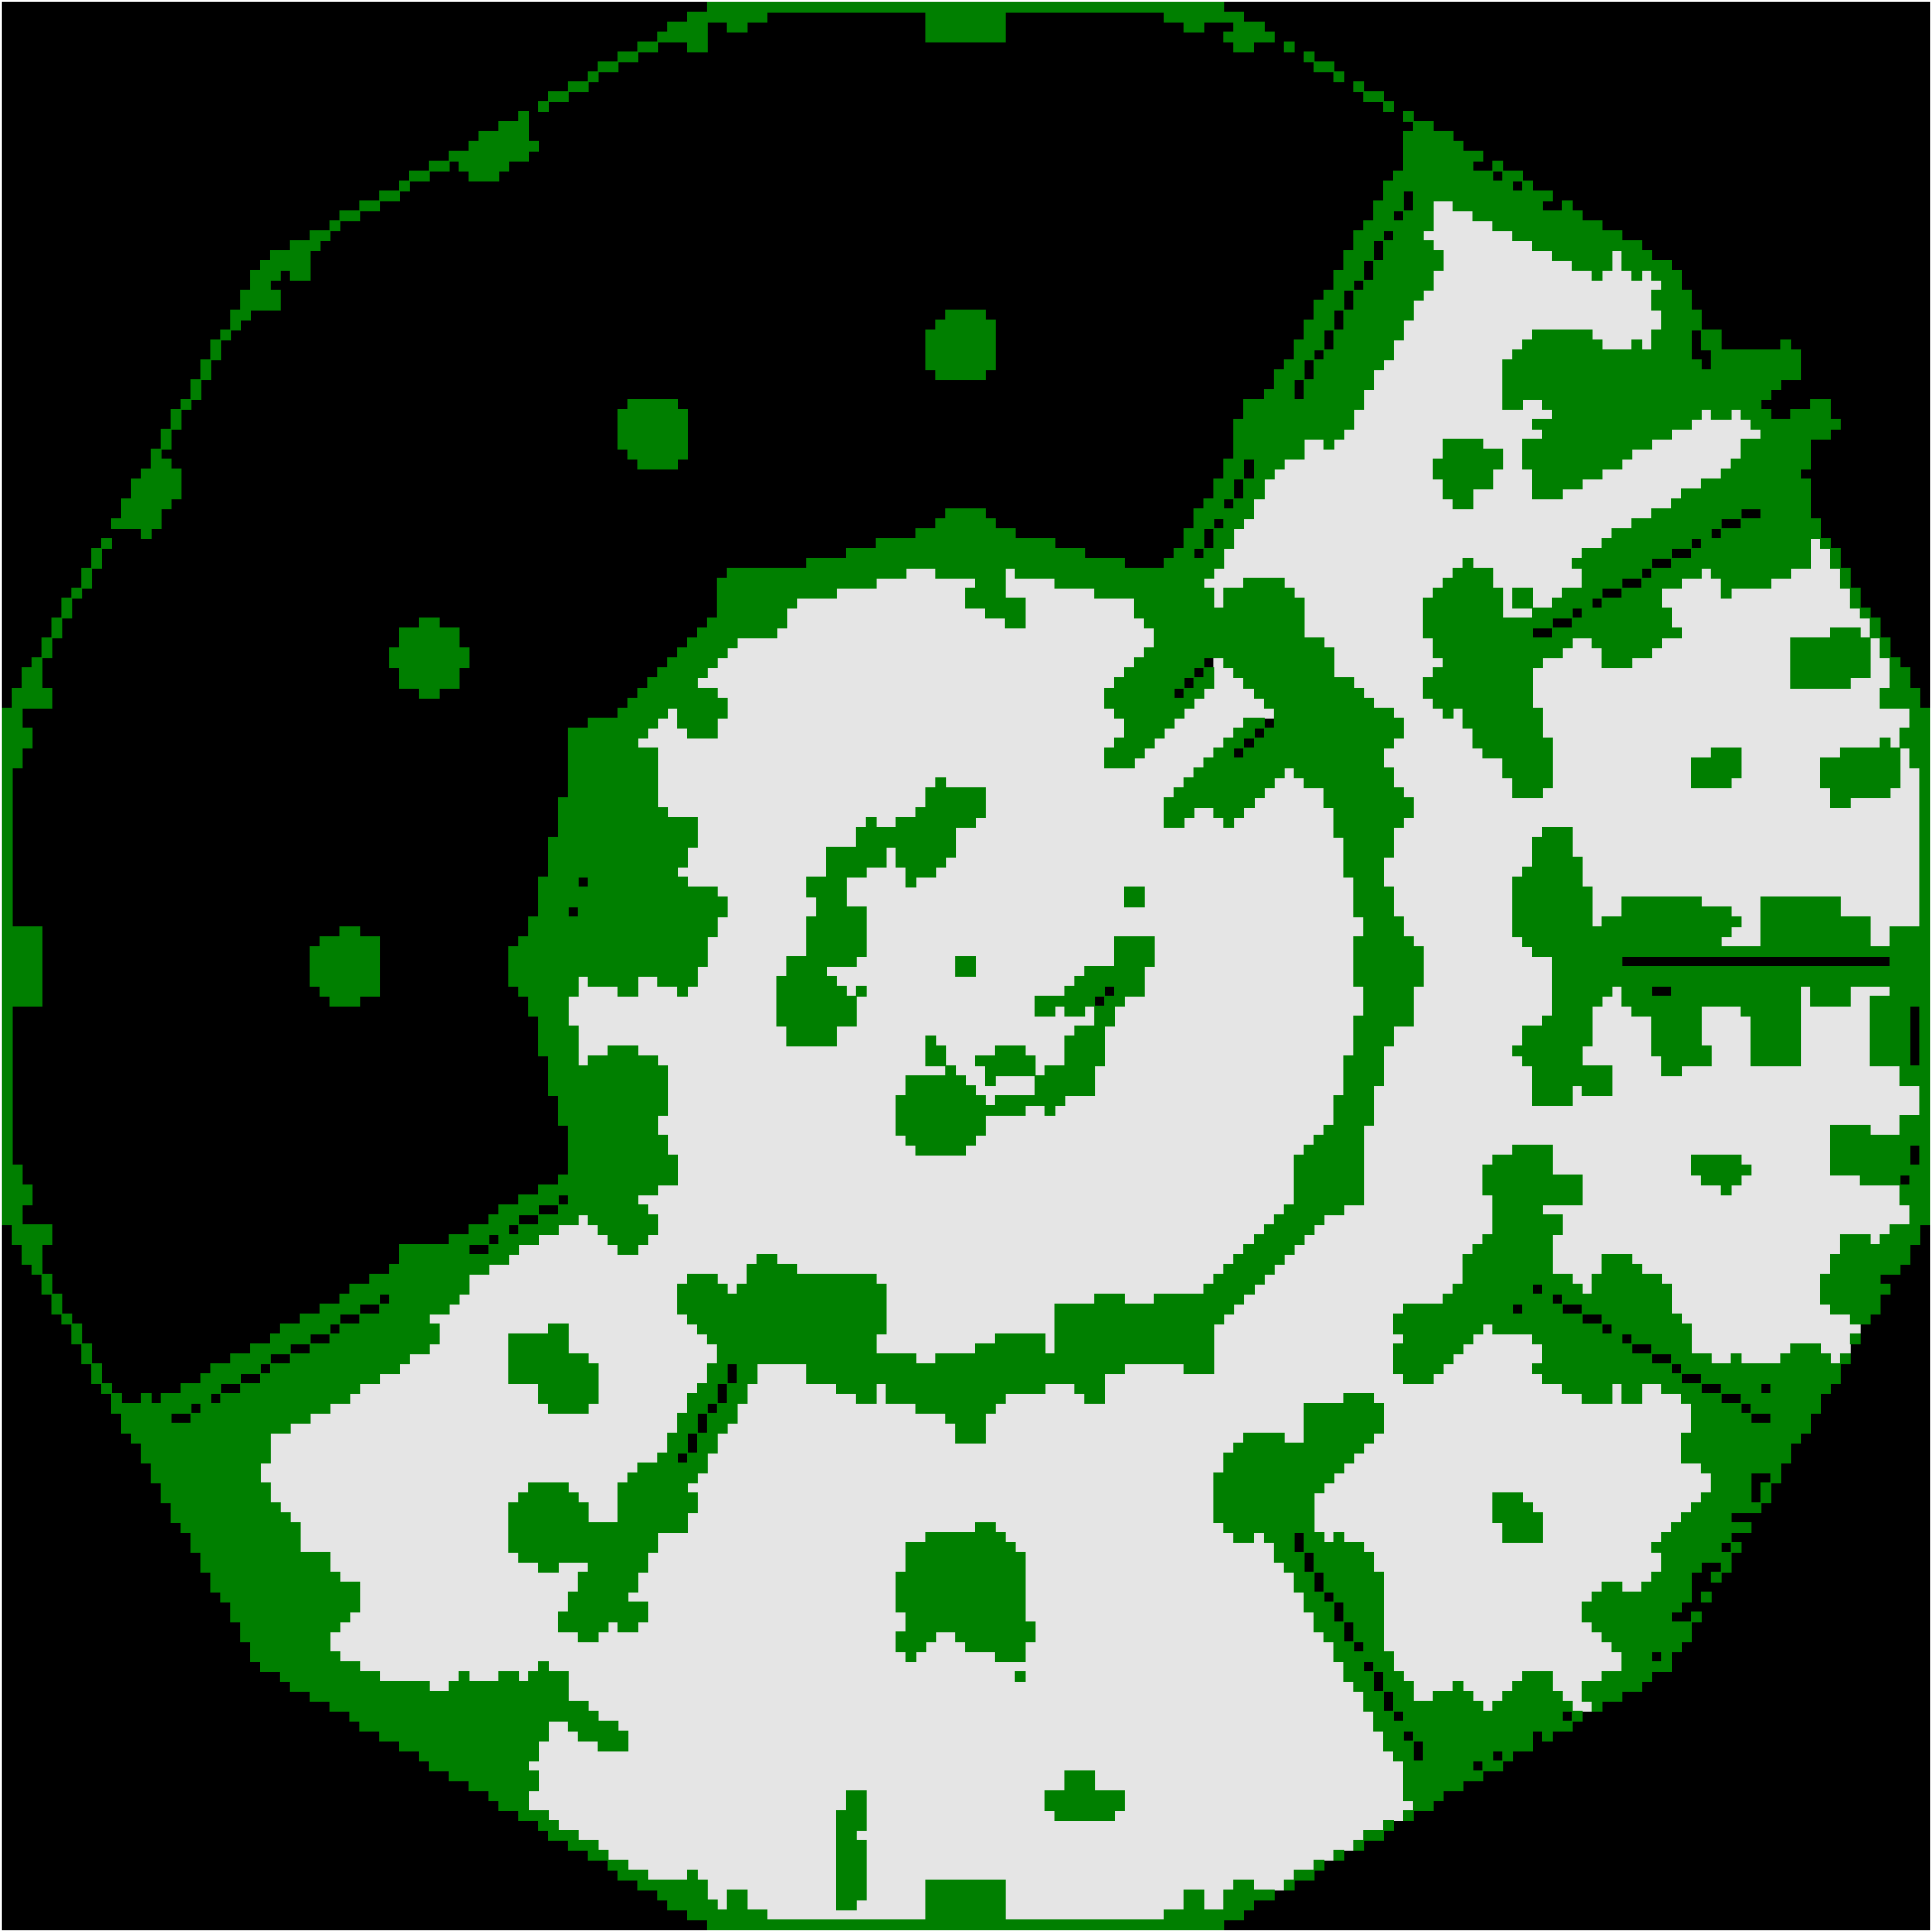
\includegraphics[width=2em]{figures/ost003d.pdf}}} 
 & 100 & 8 & $1441.40$ & \textbf{1242.43} & $43.67$ & \textbf{41.27} & $4021.85$ & \textbf{3698.54} & 3.46 & 0.10 \\
 & 200 & 8 & \textbf{3902.96} & $4000.67$ & \textbf{217.78} & $220.86$ & \textbf{30693.53} & $31512.05$ & 11.43 & 0.35 \\
 & 300 & 8 & \textbf{7970.24} & $7985.14$ & \textbf{932.51} & $968.17$ & \textbf{120037.50} & $123283.20$ & 22.36 & 0.74 \\
 & 400 & 8 & \textbf{13055.96} & $13118.59$ & $3212.46$ & \textbf{2931.14} & $312943.46$ & \textbf{303192.39} & 41.12 & 1.35 \\ \hline
\multirow{6}{*}{\vspace{1.6em}\makecell{\texttt{random}\\ 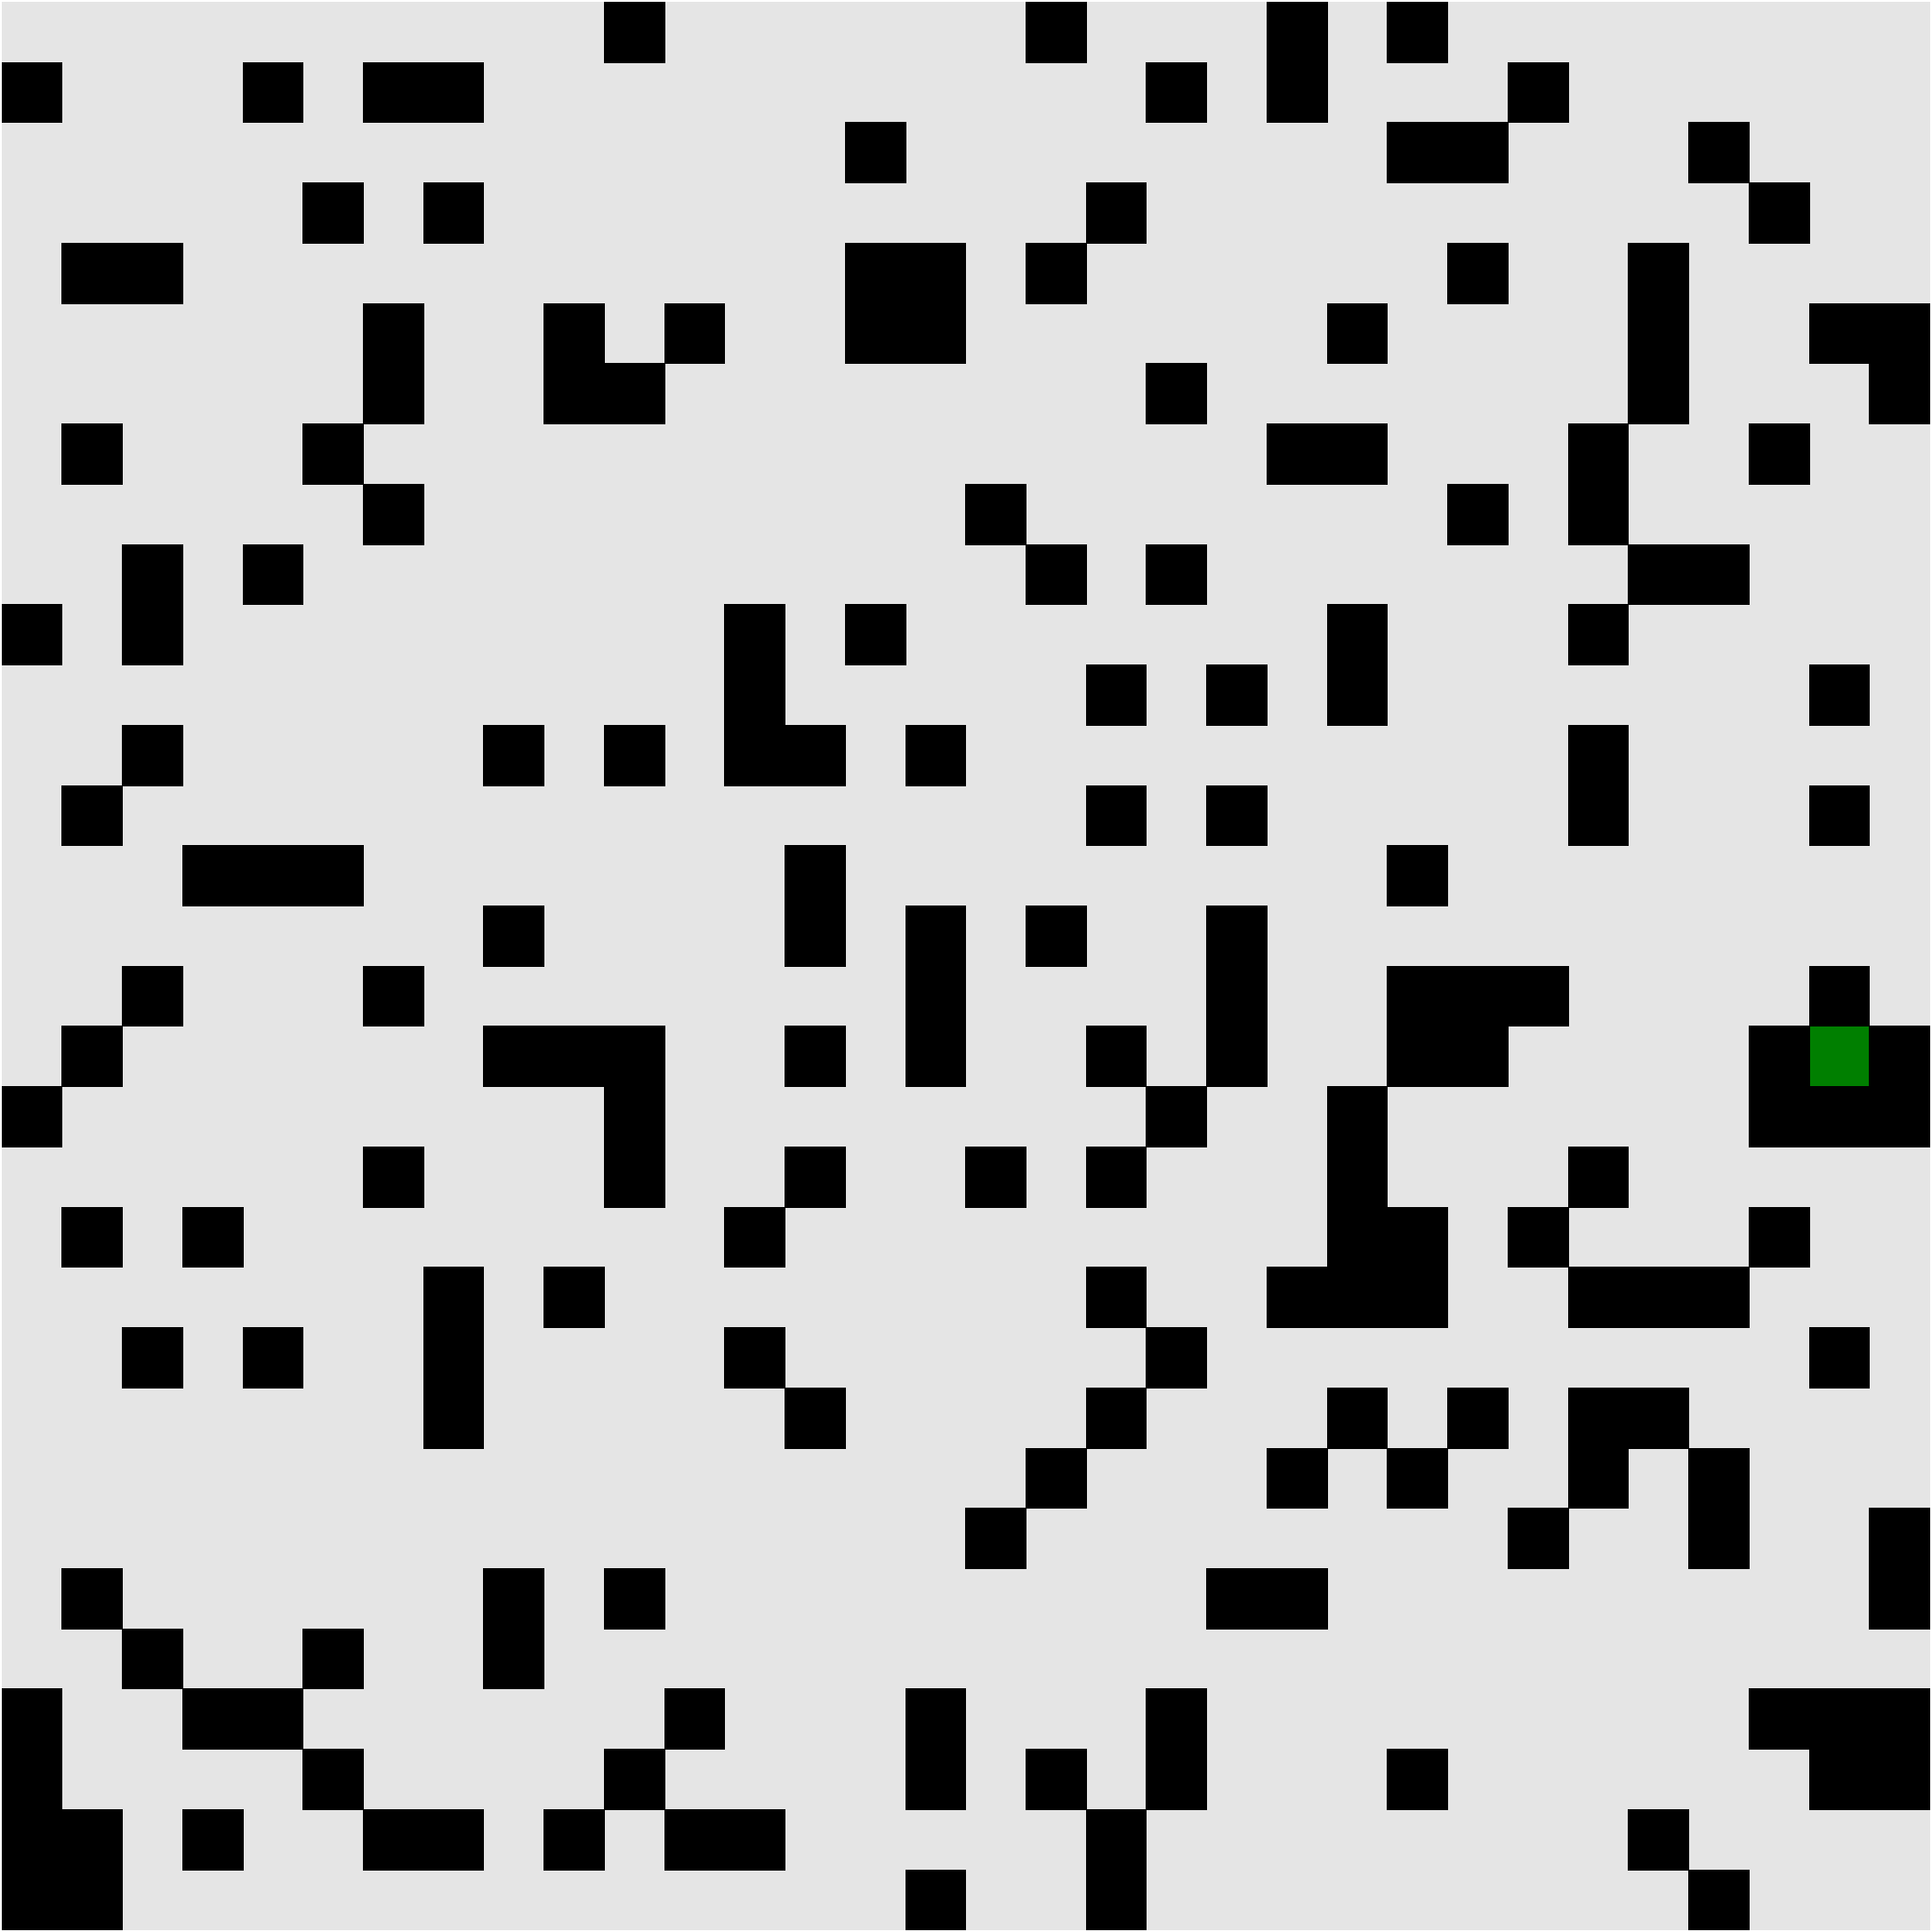
\includegraphics[width=2em]{figures/random-32-32-20.pdf}}} 
 & 50 & 16 & \textbf{106.84} & $119.77$ & \textbf{24.24} & \textbf{24.24} & \textbf{1466.29} & $1466.62$ & 0.12 & 0.00 \\
 & 100 & 16 & $467.74$ & \textbf{462.95} & \textbf{125.76} & $125.83$ & \textbf{7809.09} & $7813.90$ & 0.45 & 0.01 \\
 & 150 & 16 & $1048.85$ & \textbf{1026.20} & \textbf{342.63} & $342.75$ & $22113.44$ & \textbf{22106.02} & 1.37 & 0.05 \\
 & 200 & 16 & $1959.77$ & \textbf{1958.99} & \textbf{815.28} & $818.59$ & \textbf{54776.02} & $55069.65$ & 4.31 & 0.15 \\
 & 250 & 16 & \textbf{3496.92} & $3515.45$ & \textbf{1667.38} & $1669.86$ & $116124.45$ & \textbf{115630.32} & 17.71 & 0.61 \\ \hline
\multirow{6}{*}{\vspace{1.6em}\makecell{\texttt{warehouse}\\ 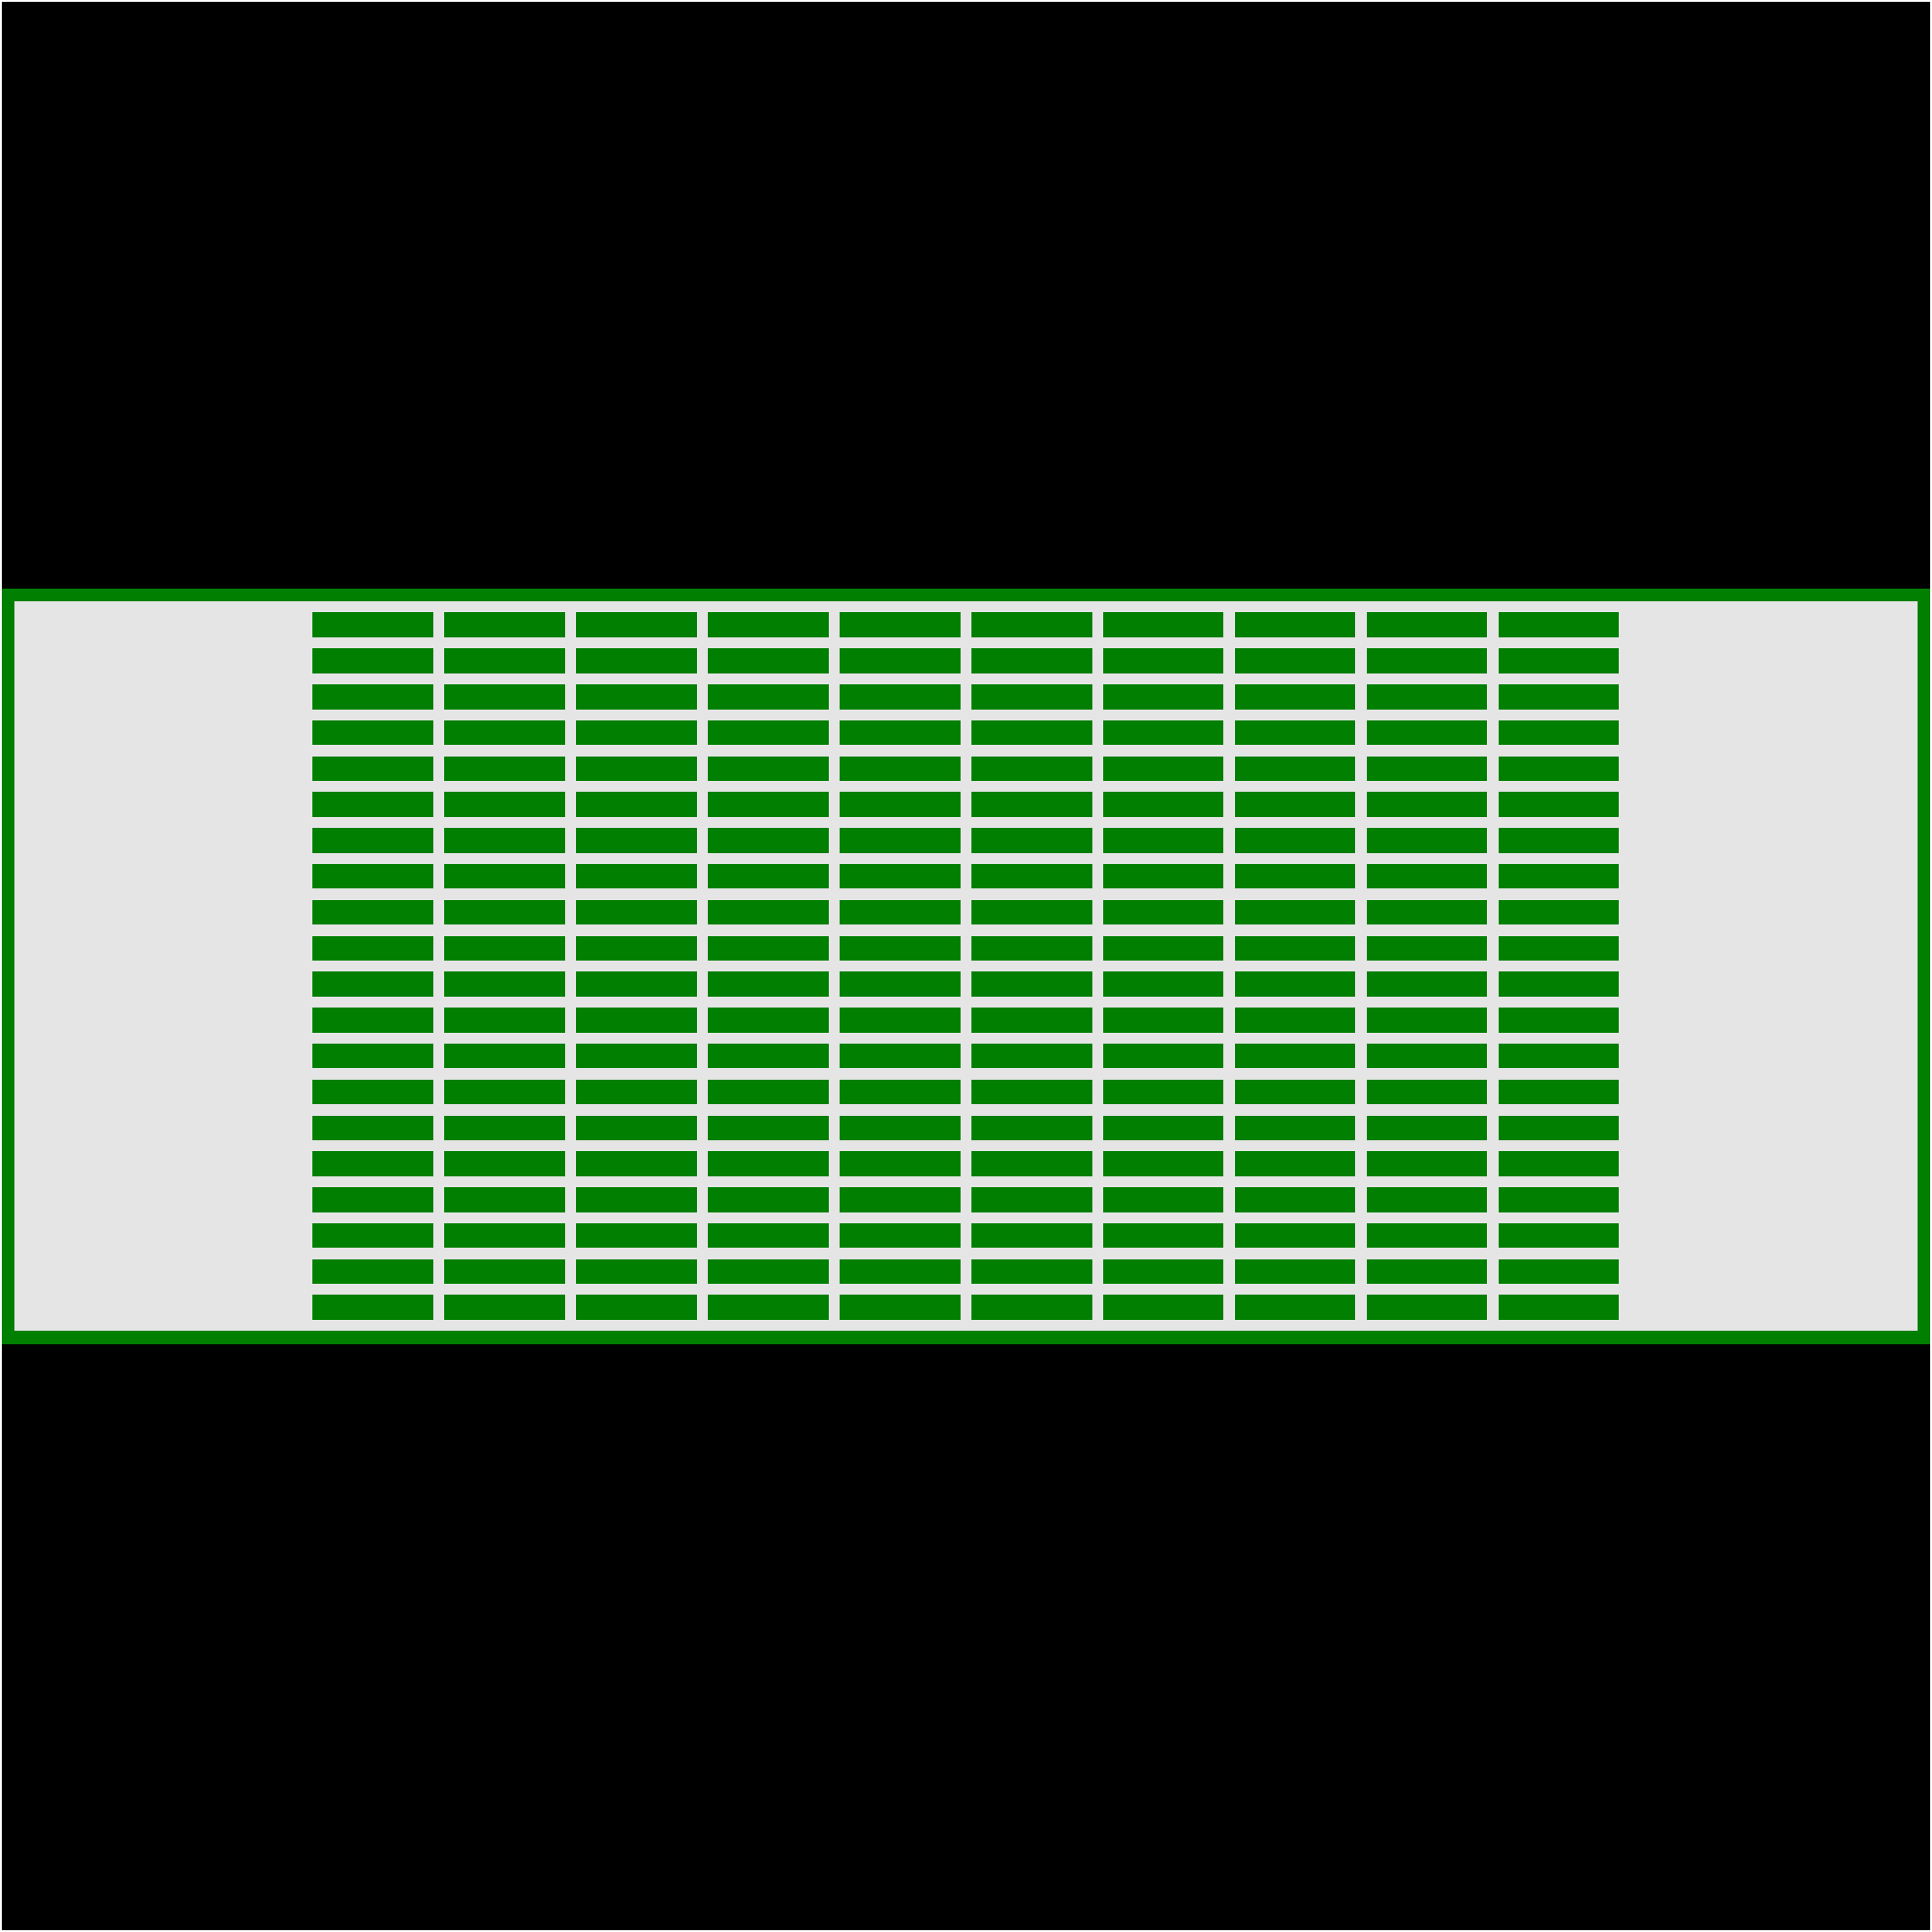
\includegraphics[width=2em]{figures/warehouse-10-20-10-2-1.pdf}}} 
 & 150 & 16 & \textbf{1844.67} & $1853.64$ & \textbf{115.86} & $116.32$ & $8481.24$ & \textbf{8370.05} & 3.32 & 0.10 \\
 & 200 & 16 & $3131.47$ & \textbf{3024.86} & $258.14$ & \textbf{257.94} & $19925.99$ & \textbf{19661.84} & 6.68 & 0.21 \\
 & 250 & 16 & \textbf{4494.93} & $4534.01$ & $464.60$ & \textbf{462.98} & \textbf{38343.22} & $38725.28$ & 12.20 & 0.43 \\
 & 300 & 16 & $6228.19$ & \textbf{6044.16} & \textbf{751.20} & $756.10$ & \textbf{66391.85} & $66866.06$ & 19.59 & 0.67 \\
 & 350 & 16 & $7914.13$ & \textbf{7696.34} & \textbf{1200.63} & $1203.22$ & \textbf{110245.29} & $110509.65$ & 30.02 & 1.07 \\ \hline
\end{tabular}
}
\end{table}

\subsection{Results}

Table~\ref{tab:benchmark-results} presents the mean values of the results obtained in our experimental evaluation of ISS-MAPF-LNS (abbreviated as ISS) and MAPF-LNS (abbreviated as LNS), focusing on the following four key metrics:

\begin{itemize}
    \item \textbf{Initial SOD:} Initial Sum of Delays (SOD) of the selected initial solution.
    \item \textbf{Final SOD:} Final SOD after optimization.
    \item \textbf{AUC:} Area Under the Curve (AUC), defined as the integral of the SOD Graph, starting from the time the initial solution is selected until the specified time limit is reached.
    \item $\boldsymbol{t}_\mathbf{init}[\boldsymbol{s}]$: Runtime required to generate initial solutions.
\end{itemize} 


The results demonstrate that for the map \texttt{empty-8-8} with 16, 24, and 32 agents, ISS tends to favor initial solutions with lower initial SODs compared to LNS. The values for 16 and 24 agents are 10.560 vs. 10.722, respectively, and 34.280 vs. 35.057 for 32 agents. However, for 32 agents, the initial SOD for LNS is 82.563, while that of ISS is 93.760. With regard to the final SOD, both algorithms achieve identical final SODs for 16 agents. However, the final SOD for ISS is marginally superior for 24 agents and slightly better for 32 agents, with values of 25.133 compared to 25.185 for LNS. Regarding the AUC values, ISS outperforms LNS in two out of three cases. It shows superior performance for 32 agents and slightly better performance for 16 agents compared to LNS.

On the map \texttt{empty-32-32} with 300, 350, 400, and 450 agents, LNS yields lower initial SODs across all number of agents compared to ISS. However, ISS outperforms LNS slightly in terms of final SOD values for 300 and 350 agents. For instance, the final SOD for 300 agents is 440.09 for ISS compared to 442.37 for LNS. However, LNS achieves significantly superior final SOD values for 400 and 450 agents. With regard to the AUC values, ISS yields significantly lower values for 300 and 350 agents than LNS, whereas LNS achieves significantly lower values for 400 and 450 agents.

For the map \texttt{ost003d} with 100, 200, 300, and 400 agents, ISS favors lower initial SODs for 200, 300, and 400 agents compared to LNS. With regard to the final SODs, ISS achieved significantly lower values for 200, and 300 agents, with particularly notable performance for 300 agents. The final SOD for 300 agents was 932.51 for ISS, in contrast to 968.17 for LNS. Moreover, ISS achieves significantly lower AUC values for 200 and 300 agents than LNS, whereas LNS yields significantly lower AUC values for 100 and 400 agents.

On the map \texttt{random} with 50, 100, 150, 200, and 250 agents, ISS achieves superior final SODs across all scenarios despite having higher initial SODs in four out of five cases. This indicates that the final solution quality is indeed dependent on the initial solution. For instance, the final SOD for 150 agents was 342.63 for ISS and 342.75 for LNS, but ISS has a significantly higher initial SOD of 1048.85 compared to 1026.20 for LNS. The AUC values for ISS are lower in three out of five cases, which highlights the benefit of initiating the optimization process from a promising initial solution.

For the map \texttt{warehouse} with 150, 200, 250, 300, and 350 agents, LNS achieves lower initial SODs in three out of five cases, while ISS outperforms LNS in three out of five cases in terms of final SOD. In particular, ISS exhibits significantly superior results for higher numbers of agents. For example, the final SOD for 350 agents is 1200.63 for ISS compared to 1203.22 for LNS. Regarding the AUC values, ISS achieves significantly superior solutions in three out of five cases lower than LNS, while LNS yields superior solutions for 150 and 200 agents.

With regard to $t_\mathrm{init}[s]$, for all maps and number of agents, the initialization times are approximately 30 times higher for ISS compared to LNS. This reflects the additional effort required to generate multiple initial solutions.

\paragraph{Key Insights:}

\begin{itemize}
    \item \textbf{Initial Solution Quality:} In many cases, the initial solutions generated by ISS exhibit lower quality. However, the final solutions achieved by ISS are of a higher quality, particularly in constrained environments such as on maps \texttt{warehouse} and \texttt{random}. 
    \item \textbf{Final Solution Quality and AUC:} In 13 out of 21 cases, the final SODs found by ISS were lower than those of LNS. Moreover, the AUC values obtained by ISS were in 12 out of 21 cases lower than those of LNS. This demonstrates the effectiveness of using LambdaMART to select promising initial solutions.
    \item \textbf{Computational Overhead:} The primary trade-off for the superior performance of ISS is the increased time required to generate initial solutions. This overhead is particularly evident in larger and more complex maps.
    \item \textbf{Seen maps:} (1) \texttt{random}: ISS performs particularly well, achieving lower final SODs in four out of five scenarios compared to LNS. This indicates the efficacy of the learned model in handling familiar environments. (2) \texttt{warehouse}: ISS shows robust performance, with lower final SODs in three out of five groups compared to LNS. Despite the longer initial solution generation time, ISS effectively optimized the solutions.
    \item \textbf{Unseen Maps:} ISS remains competitive with LNS on unseen maps like \texttt{empty-32-32} and \texttt{ost003d}, which highlights the generalization capability of the trained models.
\end{itemize}

The results indicate that the quality of the final solution in LNS is strongly correlated with its initial solution. ISS leverages its ability to select a promising solution from a diverse pool of generated initial solutions, which, although time-consuming, results in better overall optimization. The extended initial solution time for ISS is a trade-off that pays off in terms of final solution quality, particularly in complex and large maps like \texttt{warehouse}.

The strength of ISS lies in its ability to learn from training data and apply this learning to both seen and unseen scenarios, providing a robust solution even when starting late in the LNS process. This demonstrates the potential of integrating ML techniques with traditional optimization methods in MAPF problems.



\section{Conclusion and Future Work} \label{sec:conclusions}

In this work, we addressed the significant dependency of the final solution quality of MAPF-LNS on its initial solution. Despite the fact that the initial solution quality is not strongly correlated with the final solution quality, the choice of an initial solution has a substantial impact on the performance of MAPF-LNS. We proposed ISS-MAPF-LNS, a novel extension of MAPF-LNS. This approach involves executing PP with random priorities multiple times to generate a large pool of potential initial solutions. From this pool, the most promising initial solution is selected using LambdaMART, a state-of-the-art learning-to-rank algorithm, to run the LNS on.

LambdaMART was trained offline on two well-known maps, and the experimental results demonstrate that the trained model generalizes well to different numbers of agents on both seen and unseen grid maps. This indicates that our approach can effectively leverage ML to enhance the performance of MAPF-LNS.

In order to improve the robustness and generalization capability of ISS-MAPF-LNS, future research should focus on creating a more diverse set of training data. By including a wider variety of maps and scenarios during the training phase, we may reduce the model's dependence on specific map features and enhance its ability to generalize to different environments. This broader training dataset may help the model to better understand the diverse characteristics of various maps, leading to more reliable performance in new scenarios.

One of the primary challenges identified is the computational overhead associated with generating multiple initial solutions. An alternative or additional ML-based approach is to employ machine learning techniques to directly predict promising destroy sets, which are crucial components of the LNS optimization process. 

%
% ---- Bibliography ----
%
% BibTeX users should specify bibliography style 'splncs04'.
% References will then be sorted and formatted in the correct style.
%
\bibliographystyle{splncs04}
\bibliography{lspis-mapf.bib}

\end{document}
